\documentclass{report}
\usepackage{times}
\usepackage{amssymb}
\usepackage{amsmath}
\usepackage{graphicx}
\setcounter{secnumdepth}{2}
\setcounter{tocdepth}{2}
\setlength{\parindent}{0em}
\setlength{\parskip}{0.5em}
\setlength{\oddsidemargin}{0em}
\setlength{\evensidemargin}{0em}
\setlength{\textwidth}{460pt}
\setlength{\textheight}{680pt}
\setlength{\topmargin}{1em}
\setlength{\voffset}{-65pt}
\setlength{\intextsep}{1ex}
\setlength{\textfloatsep}{1ex}
\makeatletter
\newenvironment{asciibox}%
  {\begin{list}{}{%
    \setlength{\topsep}{0.5em}%
    \setlength{\parskip}{0em}%
    \setlength{\parsep}{0em}%
    \setlength{\itemsep}{0em}%
    \setlength{\rightmargin}{0em}%
    \setlength{\leftmargin}{3.0em}%
    \setlength{\labelsep}{1em}%
    \setlength{\labelwidth}{2em}%
  }\normalfont\footnotesize\item}
  {\end{list}}
\newenvironment{options}%
  {\begin{list}{}{%
    \setlength{\topsep}{1em}%
    \setlength{\parskip}{0em}%
    \setlength{\parsep}{0em}%
    \setlength{\itemsep}{1em}%
    \setlength{\rightmargin}{0em}%
    \setlength{\leftmargin}{9em}%
    \setlength{\labelsep}{1em}%
    \setlength{\labelwidth}{6em}%
    \setlength{\itemindent}{0em}}\normalfont}%
  {\end{list}}
\newenvironment{options2}%
  {\begin{list}{}{%
    \setlength{\topsep}{1em}%
    \setlength{\parskip}{0em}%
    \setlength{\parsep}{0em}%
    \setlength{\itemsep}{1em}%
    \setlength{\rightmargin}{0em}%
    \setlength{\leftmargin}{13em}%
    \setlength{\labelsep}{1em}%
    \setlength{\labelwidth}{10em}%
    \setlength{\itemindent}{0em}}\normalfont}%
  {\end{list}}
%
% ...Figure,table etc captions
%
\renewcommand{\@makecaption}[2]{%
	\vspace{0.6em}\begin{center}{\parbox{0.9\linewidth}%
        {\small\textbf{#1.} #2}}\end{center}%
}
\makeatother
%
\usepackage{url}
\usepackage[%
  pdfauthor={Cornelis Dullemond},
  pdftitle={Manual for RADMC-3D},
  pdfstartview=FitH,
  linkcolor=blue,
  anchorcolor=blue,
  citecolor=blue,
  filecolor=blue,
  menucolor=blue,
  urlcolor=blue,
  colorlinks=true,
  final=true]{hyperref}
%
\begin{document}

\centerline{\Huge \bf Manual for RADMC-3D}

\vspace{1em}

\centerline{\Huge \bf Version 0.41}

\vspace{4em}

\centerline{\huge \bf C.P.~Dullemond}

\vspace{2em}

\centerline{\Large \bf with substantial contributions from:}

\vspace{0.3em}

\centerline{\Large \bf M.~Min, A.~Juhasz, A.~Pohl, R.~Shetty, F.~Sereshti, T.~Peters, B.~Commercon, A.~Ziampras}

\vspace{2em}

\centerline{\Large \bf and testing and feedback by:}

\vspace{0.3em}

\centerline{\Large \bf D.~Harsono, R.~Rolffs, L.~Szucs, S.~Andrews, S.~Offner, C.~Beaumont}
\centerline{\Large \bf K.~Rosenfeld, S\o ren Frimann, Jon Ramsey, Seokho Lee, Blake Hord}
\centerline{\Large \bf and others}

\vspace{2em}

\centerline{\large This code benefitted from financial support by the german
  science foundation (DFG)}
\centerline{\large under the Schwerpunkt Programm (SPP) ``Interstellar
  Medium''}

\vspace{6em}




\centerline{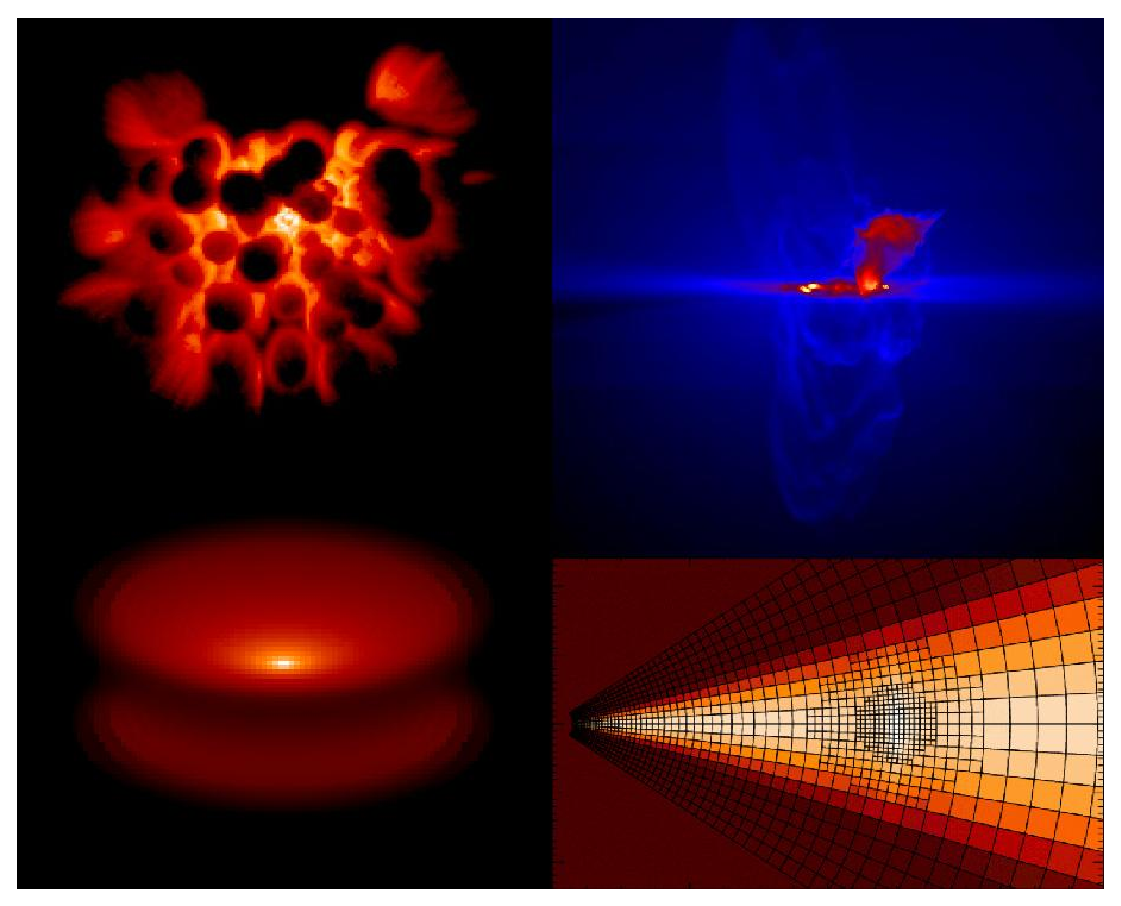
\includegraphics[width=0.9\textwidth]{coverim_lowres.eps}}

\clearpage
\mbox{}
\vfill
\noindent{\it {\bf Front page images:} Simulations with RADMC-3D. Upper-left:
A simple model of a clumpy dust ``torus'' around an active galactic nucleus.
Upper-right: A simulation of high-mass star formation by Thomas Peters (ITA,
University of Heidelberg, 2010) using the FLASH MHD code. Lower-left: A
simple 2-D axisymmetric model of a protoplanetary disk seen in scattered
light. Lower-right: An example of the kind of grid refinement possible with
RADMC-3D.}



\clearpage

\setcounter{tocdepth}{3}

\tableofcontents

\clearpage


%----------------------------------------------------------------------------
%                       CHAPTER: INTRO
%----------------------------------------------------------------------------
\chapter{Introduction, copyright and disclaimer}
\section{Introduction}
RADMC-3D is a software package for astrophysical radiative transfer
calculations in arbitrary 1-D, 2-D or 3-D geometries. It is mainly written
for continuum radiative transfer in dusty media, but also includes
modules for gas line transfer and gas continuum transfer.

RADMC-3D is a new incarnation of an older software package called RADMC.
The original RADMC package was written in Fortran 77 and was only for
axially symmetric problems in spherical coordinates. Because it was written
in Fortran 77, the arrays had a fixed maximum size, so whenever a new grid
was necessary, the code had to be recompiled. RADMC was also ageing in many
other ways, in the sense that it used input formats that stemmed from the
very early developing phase, and were not particularly practical. Also,
RADMC's limitation to axisymmetric configurations and rigid gridding made it
not capable of dealing with more complex 3-D models that are now becoming
ever more mainstream. For these reasons I decided to make a huge make-over
of the code, or more precise: to build a new incarnation of RADMC, called
RADMC-3D, almost completely from scratch. 

At the moment RADMC-3D is still in the development phase, but is is already
reasonably mature. Here is a list of current and planned features. Those
features that are now already working are marked with [+], while those which
are not yet (!!) built in are marked with [-]. Those that are currently
being developed are marked with [.] and those that are ready, but are still
in the testing phase are marked with [t].

\begin{itemize}
\item Coordinate systems:
  \begin{itemize}
    \item[][+] Cartesian coordinates (3-D)
    \item[][+] Spherical coordinates (1-D, 2-D and 3-D)
  \end{itemize}
\item Gridding systems (regular and adaptive mesh refinement grids are
  available for cartesian {\em and} spherical coordinates):
  \begin{itemize}
    \item[][+] Regular
    \item[][+] Adaptive Mesh Refinement: oct-tree style
    \item[][+] Adaptive Mesh Refinement: layered ('patch') style
    %\item[][.] Tetrahedral gridding {\em [being developed]}
    \item[][-] Voronoi gridding {\em [To be implemented on request]}
  \end{itemize}
\item Radiation mechanisms:
  \begin{itemize}
    \item[][+] Dust continuum, thermal emission
    \item[][t] Dust continuum scattering:
      \begin{itemize}
      \item[][+] ...in isotropic approximation
      \item[][+] ...with full anisotropy
      \item[][+] ...with full Stokes and Polarization
      \end{itemize}
    \item[][-] Dust quantum heated grains {\em [To be implemented on request]}
    \item[][t] Polarized dust emission by aligned grains {\em [first test version]}
    %\item[][-] Polarized line emission {\em [planned]}
    \item[][+] Gas line transfer (LTE)
    \item[][+] Gas line transfer (non-LTE: LVG)
    \item[][+] Gas line transfer (non-LTE: LVG + Escape Probability)
    \item[][-] Gas line transfer (non-LTE: full transfer)
    \item[][+] Gas line transfer with user-defined populations
    \item[][+] Gas continuum opacity and emissivity sources
  \end{itemize}
\item Radiation netto sources for continuum:
  \begin{itemize}
    \item[][+] Discrete stars positioned at will
    \item[][t] Continuous 'starlike' source
    \item[][t] Continuous 'dissipation' source
    \item[][t] External 'interstellar radiation field'
  \end{itemize}
\item Imaging options:
  \begin{itemize}
    \item[][+] Easy-to-use IDL front-end widget interface for imaging
    \item[][+] Observer from 'infinite' distance
    \item[][+] Zoom-in at will
    \item[][+] Flux-conserving imaging, i.e. pixels are recursively refined
    \item[][+] A movie-making tool
    \item[][+] Multiple wavelengths in a single image
    \item[][+] Local observer with perspective view (for PR movies!)
  \end{itemize}
\item Spectrum options:
  \begin{itemize}
    \item[][+] SED spectrum (spectrum on 'standard' wavelength grid)
    \item[][+] Spectrum on any user-specified wavelength grid
    \item[][+] Spectrum of user-specified sub-region (pointing)
    \item[][t] Specification of size and shape of a primary 'beam' for spectra
  \end{itemize}
\item User flexibility:
  \begin{itemize}
    \item[][+] Free model specification via tabulated input files
    \item[][+] Easy special-purpose compilations of the code (optional)
  \end{itemize}
\item Front-end IDL packages:
  \begin{itemize}
    \item[][+] Example model setups
    \item[][+] Image viewing GUI (graphical user interface). NOTE: As of now
      also a non-IDL stand-alone image viewing GUI (in Qt) is available.
  \end{itemize}
\item Front-end Python packages:
  \begin{itemize}
    \item[][+] Python RADMC-3D library (author: A.~Juhasz)
  \end{itemize}
\item Miscellaneous:
  \begin{itemize}
    \item[][+] Stars can be treated as point-sources or as spheres
    \item[][+] Option to calculate the mean intensity $J_\nu(\vec x)$ in the model
    \item[][+] OpenMP parallellization of the Monte Carlo
  \end{itemize}
\end{itemize}


\section{Version tracker}
The RADMC-3D software package in under continuous development. A very
detailed development log-book can be found in the {\small\tt
  src/Radmc\_3D\_LOG.txt} text file, but this may be too detailed for most
users. A more user-friendly overview of the development history can be 
found in this manual, in appendix \ref{chap-development-history}.


\section{Copyright and disclaimer} 
RADMC-3D was developed from 2007 to 2010/2011 at the Max Planck Institute
for Astronomy in Heidelberg, funded by a Max Planck Research Group grant
from the Max Planck Society. As of 2011 the development continues at the
Institute for Theoretical Astrophysics (ITA) of the Zentrum f\"ur Astronomy
(ZAH) at the University of Heidelberg.

{\bf The use of this software is free of charge. However, it is not allowed
  to distribute this package without prior consent of the lead author
  (C.P. Dullemond). Please refer any interested user to the web site of this
  software where the package is available, which is currently:}

{\bf http://www.ita.uni-heidelberg.de/~dullemond/software/radmc-3d/}

{\bf IMPORTANT NOTICE 1: I/We reject all responsibility for the use of this
  package. The package is provided as-is, and we are not responsible for any
  damage to hardware or software, nor for incorrect results that may result
  from the software. The user is fully responsible for any results from this
  code, and we strongly recommend thorough testing of the code before using
  its results in any scientific papers.}

{\bf IMPORTANT NOTICE 2: Any publications which involve the use of this
  software must mention the name of this software package and cite the
  accompanying paper once it is published (Dullemond et al.\ in prep), or
  before that the above mentioned web site.}

{\bf IMPORTANT NOTICE 3: If you use this software, you may want to notify
  the lead author (C.P. Dullemond) so that you are put on an email list. 
  This ensures that you are always up to date with major bug reports and
  major updates. This mail list is only used for important enough news,
  so you will not be flooded with emails and you can always unsubscribe.}


%----------------------------------------------------------------------------
%                       CHAPTER: QUICK START
%----------------------------------------------------------------------------
\chapter{Quick-Start}\label{chap-quick-start}
In general I recommend reading the manual fully, but it is often useful
to get a quick impression of the package with a quick-start. To make your
first example model, this is what you do:
\begin{enumerate}
\item When you read this you have probably already unzipped this package.
  You should find, among others, a {\small\tt src/} directory and a
  {\small\tt examples/} directory. Go into the {\small\tt src/} directory.
\item Edit the {\small\tt src/Makefile} file, and make sure to set the
  {\small\tt FF} variable to the Fortran-90 compiler you have installed on
  your system.
\item Type {\small\tt make}. If all goes well, this should compile the
  entire code and create an executable called {\small\tt radmc3d}.
\item Type {\small\tt make install}. If all goes well this should try to
  create a link to {\small\tt radmc3d} in your {\small\tt $\sim$/bin/}
  directory. If this directory does not exist, it will ask to make one.
\item Make sure to have the {\small\tt $\sim$/bin/} directory in your path.
  If you use, for instance, the {\small\tt tcsh} shell, you do this by
  setting the {\small\tt path} variable: {\small\tt set path = ( $\sim$/bin
    \$path )} in your {\small\tt $\sim$/.tcshrc} file. If you change these
  things you may have to open a new shell to make sure that the shell now
  recognizes the new path.
\item Check if the executable is OK by typing {\small\tt radmc3d} in the
  shell. You should get a small welcoming message by the code.
\item Now enter the directory {\small\tt examples/run\_simple\_1/}. 
\item Copy all standard IDL (see Section \ref{sec-requirements} about IDL)
  routines from the {\small\tt ../../idl/} directory into the current
  directory by typing in the tcsh or bash shell {\small\tt cp
    ../../idl/*.pro ./}. {\em NOTE: This is a quick-and-dirty way of using
    the IDL routines, only meant to get the stuff running quickly without
    going through the somewhat more involved IDL routines installation
    procedure described in Section \ref{sec-install-idlscripts}. For the the
    proper use of the RADMC-3D package, it is recommended to follow the
    procedures described in Section \ref{sec-install-idlscripts}.}
\item Enter IDL. 
\item Type (in IDL) {\small\tt .r problem\_setup.pro}, and after that 
{\small\tt exit} to exit IDL again.
\item Type {\small\tt radmc3d mctherm}. This should let the code do a Monte
  Carlo run. You should see {\small\tt Photon nr 1000}, followed by
  {\small\tt Photon nr 2000}, etc until you reach {\small\tt Photon nr
    1000000}. The Monte Carlo modeling for the dust temperatures has now
  been done.
\item Go into IDL again and type {\small\tt .r viewimage.pro} followed by
  {\small\tt viewimage}. This should bring an image viewer on the screen and
  show what the simple model looks like when rendered at some
  angle\footnote{Note: on some systems there is an apparent problem with the
    communication pipe between {\small\tt radmc3d} and IDL which causes
    things to freeze. Try typing {\small\tt viewimage,/nochild} in that
    case, which should fix the problem, although the viewer may then be
    substantially slower. I am working on figuring out how the problem can
    be fixed, but have so far been not succesful.}. The model is very
  simple: a spherical blob, so do not expect to see much in this simple
  example.
\end{enumerate}
If you experience troubles with the above steps, and you cannot fix it,
please read the next chapters for more details. 

{\em Tip: If the code unexpectedly quits or freezes while using} {\small\tt
  viewimage}, {\em please have a look at the file} {\small\tt radmc3d.out}
{\em which contains the messages that RADMC-3D outputs. This may give hints
  what went wrong. Note that this file is only written if RADMC-3D is used
  in child mode, which is the case when it is spawned from viewimage.
  Otherwise this output will be written to screen. Also, when viewimage is
  called with the option} {\small\tt ,/nochild} {\em the output will also be
  written to screen instead of the file} {\small\tt radmc3d.out}.




%----------------------------------------------------------------------------
%                  CHAPTER: OVERVIEW OF RADMC-3D PACKAGE
%----------------------------------------------------------------------------
\chapter{Overview of the RADMC-3D package}
\section{Introduction}
The RADMC-3D code is written in fortran-90 and should compile with most f90
compilers without problems. It needs to be compiled only once for each
platform. {\em Note that the code is developed for Unix-based systems such
  as linux machines or Mac OS X machines. It may also work on Windows
  machines, but this is not guaranteed, and throughout this manual a
  Unix-based machine is assumed, with a csh, tcsh or bash shell. User-level
  knowledge of Unix-like operating systems is required.}

The executable is called {\small\tt radmc3d} and it performs all the model
calculations of the RADMC-3D package, for instance the Monte Carlo
simulations, ray-tracing runs (images, spectra), etc. There is also a set of
useful subroutines written in the IDL\footnote{IDL is a commercial data
  processing package used frequently among astrophysicists. See {\small\tt
    http://www.ittvis.com/idl/} for more information.} language to use the
{\small\tt radmc3d} code, but {\small\tt radmc3d} can also run without
IDL. In that case the user will have to write his/her own pre- and
post-processing subroutines in e.g.\ python or other data processing
languages.

\section{Requirements}\label{sec-requirements}
This package runs under linux/unix/MacOSX, but has not been tested under
Windows. The following pre-installed software is required:
\begin{itemize}
\item {\small\tt make} or {\small\tt gmake}\\
  This is the standard tool for compiling packages on all Unix/Linux-based
  systems.
\item {\small\tt perl}\\
  This is a standard scripting language available on most or all
  Unix/Linux-based systems. If you are in doubt: type {\small\tt which perl}
  to find the location of the {\small\tt perl} executable. See {\small\tt
    http://www.perl.org/} for details on perl, should you have any
  problems. But on current-day UNIX-type operating systems perl is nearly
  always installed in the {\small\tt /usr/bin/} directory.
\item {\small\tt A fortran-90 compiler}\\
  Preferably the {\small\tt gfortran} compiler (which the current
  installation assumes is present on the system). Website: {\small\tt
    http://gcc.gnu.org/fortran/}. Other compilers may work, but have not
  been tested yet.
\item {\small\tt An OpenMP-fortran-90 compiler}\\
  Only needed if you want to use the parallelized OpenMP version for the
  thermal Monte Carlo (from version 0.38 onward). Preferably the {\small\tt
    GNU OpenMP/GOMP} compiler which is an implementation of OpenMP for the
  Fortran compiler in the GNU Compiler Collection. Websites: {\small\tt
    http://openmp.org/wp} and {\small\tt http://gcc.gnu.org}. Other
  compilers may work, but have not been tested yet.
\item {\small\tt The IDL package (Interactive Data Language)}\\
  {\small\tt IDL} is a software package similar to MatLab, and it is not
  free.  While RADMC-3D can be used without IDL, all examples and all
  post-processing scripts are written in IDL, so it would require the user
  to rewrite them into other languages (fortran, c, c++, perl, python or
  whatever). The website for IDL is: {\small\tt http://www.ittvis.com/}. If
  {\small\tt IDL} is not present on your system, and your system
  administrators cannot install this package due to lack of funding, you can
  also use an open source clone called {\small\tt GDL} (Gnu Data Language)
  which can be readily downloaded from the web ({\small\tt
    http://gnudatalanguage.sourceforge.net/}). This GDL package misses some
  libraries and features, but the RADMC-3D code can be used with GDL with
  the exception that the Graphical User Interfaces of RADMC-3D (such as
  viewimage.pro) cannot be used.
\end{itemize}
Note that the Monte Carlo code RADMC-3D itself is in Fortran-90. Only the
creation of the input files (and hence the problem definition) and the
analysis of the output files is done in IDL. The user is of course invited
to use other ways to create the input files for RADMC-3D if he/she is not
able to use IDL. Therefore IDL are not strictly required for the use of this
code.


\section{The archive, how to unzip it, and what it contains}
The package of RADMC-3D is packed in a zip archive called {\small\tt
  radmc-3d\_v*.**\_\#\#.\#\#.\#\#.zip} where the {\small\tt *.**} is the version
number and {\small\tt \#\#.\#\#.\#\#} is the date of this version in dd.mm.yy
format. To unpack on a linux, unix or Mac OS X machine you type:
{\small\begin{verbatim}
unzip <this archive file>
\end{verbatim}}
i.e.\ for example for radmc-3d\_v0.07\_27.07.09.zip you type
{\small\begin{verbatim}
unzip radmc-3d_v0.07_29.07.09.zip
\end{verbatim}}
A directory {\small\tt radmc-3d} is created which has the following subdirectory
structure:
{\small\begin{verbatim}
radmc-3d/
   src/
   idl/
   examples/
      run_simple_1/
      run_simple_1_userdef/
      run_simple_1_userdef_refined/
      .
      .
      .
   manual/
\end{verbatim}}
The first directory, {\small\tt src/}, contains the fortran-90 source code for
RADMC-3D. The second directory, {\small\tt idl/}, contains a set of IDL routines
that are useful for model preparation and post-processing. The third
directory contains a series of example models. The fourth directory contains
this manual.

{\bf NOTE:} As of version 0.38 there is also Python support. This was
developed by Attila Juhasz. As of version 0.40 Python (version 2.7) is now
the standard front-end, but we still keep the IDL routines as secondary
analysis toolset.


\section{Units: RADMC3D uses CGS}
The RADMC-3D package is written such that all units are in CGS (length in
cm, time in sec, frequency in Hz, energy in erg, angle in steradian). There
are exceptions:
\begin{itemize}
\item Wavelength is usually written in micron
\item Sometimes angles are in degrees (internally in radian, but input as degrees)
\end{itemize}




%----------------------------------------------------------------------------
%                  CHAPTER: COMPILATION AND INSTALLATION
%----------------------------------------------------------------------------
\chapter{Compilation and installation of radmc3d}
\label{chap-compilation}
% 
Although the RADMC-3D package contains a lot of different software,
the main code is located in the {\small\tt src/} directory, and is
written in Fortran-90. The executable is {\small\tt radmc3d}. Here
we explain how to compile the fortran-90 source codes and create 
the executable {\small\tt radmc3d}.


\section{Compiling the code with 'make'}\label{sec-makeing}
To compile the code, enter the {\small\tt src/} directory in your shell (we assume
a tcsh shell here, but bash or other Unix-shells are also fine). You now
{\em may} need to edit the {\small\tt Makefile} in this directory using your favorite
text editor and replace the line
{\small\begin{verbatim}
FF = gfortran
\end{verbatim}}
with a line specifying your own compiler. If, of course, you use gfortran,
you can keep this line. But if you use, e.g., ifort, then replace the above
line by
{\small\begin{verbatim}
FF = ifort
\end{verbatim}}
If you save this file, and you are back in the shell, you can compile the
radmc3d code by typing
{\small\begin{verbatim}
make
\end{verbatim}}
in the shell. If all
goes well, you have now created a file called {\small\tt radmc3d} in the {\small\tt
  src/} directory.

\subsection{Compiling the OpenMP version}\label{sec-makeomp}  
To compile the code of version 0.38 or higher, including the parallelized
OpenMP part, enter the {\small\tt src/} directory in your shell and edit the
{\small\tt Makefile} in this directory by adding {\small\tt -fopenmp}
(assumption that you use GNU OpenMP, cf. Sect. \ref{sec-requirements}) to
either {\small\begin{verbatim} OPTIM = -O2 -fopenmp
\end{verbatim}}

or to
{\small\begin{verbatim}
FF = gfortran -fopenmp
\end{verbatim}}

After saving the file, you can compile the {\small\tt radmc3d} code by
typing {\small\tt make} in the shell, as described above. If you prefer to
use another compiler, please have a look at {\small\tt
  http://openmp.org/wp/openmp-compilers/}.

\section{The install.perl script}
If instead of typing just `make' you type
{\small\begin{verbatim}
make install
\end{verbatim}}
(or you first type `make' and then `make install', it's the same), then
in addition to creating the executable, it also automatically executes 
a perl script called
{\small\tt install.perl} (located also in the {\small\tt src/} directory) that installs
the code in such a way that it can be conveniently used in any
directory. What it does is:
\begin{enumerate}
\item It checks if a {\small\tt bin/} directory is present in your home
  directory (i.e.\ a $\sim${\small\tt /bin/} directory). If not, it asks if
  you want it to automatically make one.
\item It checks if the $\sim${\small\tt /bin/} directory is in the 'path' of
  the currently used shell. This is important to allow the computer to look
  for the program 'radmc3d' in the $\sim${\small\tt /bin/} directory. If you
  use a csh or tcsh shell, then you can add the following line to your
  $\sim${/.tcshrc} file: {\small\begin{verbatim} set path=($HOME/bin $path)
\end{verbatim}}
\item It creates a file {\small\tt radmc3d} in this $\sim${\small\tt /bin/}
  directory with the correct executable permissions. This file is merely a
  dummy executable, that simply redirects everything to the true {\small\tt
    radmc3d} executable located in your current {\small\tt src/}
  directory. When you now open a new shell, the path contains the
  $\sim${\small\tt /bin/} directory, and the command {\small\tt radmc3d} is
  recognized. You can also type {\small\tt source $\sim${/.tcshrc}} followed
  by {\small\tt rehash}. This also makes sure that your shell recognizes the
  {\small\tt radmc3d} command.
\item It checks if a {\small\tt python/} subdirectory exists in the above
  mentioned {\small\tt bin} directory, i.e.\ a $\sim${\small\tt /bin/python/}
  directory. If not, it asks if you want it to automatically create one.
\item If yes, then it will copy all the files ending with {\small\tt .py} in
  the {\small\tt python/radmc3dPy/} directory of the distribution to that
  $\sim${\small\tt /bin/python/radmc3dPy/} directory. This is useful to
  allow you to make an {\small\tt PYTHONPATH} entry to allow python to find
  these python scripts automatically (see Section
  \ref{sec-install-pythonscripts}).
\item It checks if a {\small\tt idl/} subdirectory exists in the above
  mentioned {\small\tt bin} directory, i.e.\ a $\sim${\small\tt /bin/idl/}
  directory. If not, it asks if you want it to automatically create one.
\item If yes, then it will copy all the files ending with {\small\tt .pro}
  in the {\small\tt idl/} directory of the distribution to that
  $\sim${\small\tt /bin/idl/} directory. This is useful to allow you to make
  an {\small\tt IDL\_PATH} entry to allow idl to find these idl scripts
  automatically (see Section \ref{sec-install-idlscripts}).
\end{enumerate}
Note that this perl script installs the code only for the user that installs
it. A system-wide installation is, in my view, not useful, because the code
package is not very big and it should remain in the control of the user
which version of the code he/she uses for each particular problem.

If all is 'normal', then the {\small\tt perl.install} script described here is
called automatically once you type {\small\tt make install} following the
procedure in Section \ref{sec-makeing}.

Before the installation is recognized by your shell, you must now either
type {\small\tt rehash} in the shell or simply open a new shell. 

How do you know that all went OK? If you type {\small\tt radmc3d} in the
shell the RADMC-3D code should now be executed and give some comments. It
should write:
\begin{asciibox}\begin{verbatim}

================================================================
          WELCOME TO RADMC-3D: A 3-D CONTINUUM RT SOLVER

           This is the 3-D version of the 2-D RADMC code
                 (c) 2008 Cornelis Dullemond
================================================================

 Nothing to do... Use command line options to generate action:
   mctherm        : Do Monte Carlo simul of thermal radiation
   mcscat         : Do Monte Carlo simul only for scattering
   spectrum       : Make continuum spectrum
   image          : Make continuum image

\end{verbatim}\end{asciibox}
on the screen (or for newer versions of RADMC-3D perhaps some more
or different text). This should also work from any other directory.


\section{What to do if this all does not work?}
In case the above compilation and installation does not work, here is a 
proposed procedure to do problem hunting:
\begin{itemize}
\item First, answer the following questions:
  \begin{itemize}
    \item Did you type {\small\tt make install} in the {\small\tt src/}
      directory? I mean, did you not forget the {\small\tt install} part?
    \item Did you put $\sim${\small\tt /bin/} in your path (see above)?
    \item If you just added $\sim${\small\tt /bin/} to your path, did you
      follow the rest of the procedure (either closing the current shell and
      opening a new shell or typing the {\small\tt source} and {\small\tt
        rehash} commands as described above)?
  \end{itemize}
  If this does not help, then continue:
\item Close the shell, open a new shell.
\item Go to the RADMC-3D {\small\tt src/} directory.
\item Type {\small\tt ./radmc3d}. This should give the above message. If
  not, then make sure that the compilation went right in the first place:
  \begin{itemize}
  \item Type {\small\tt rm -f radmc3d}, to make sure that any old executable
    is not still present.
  \item Type {\small\tt make clean}. This should return the sentence
    {\small\tt OBJECT and MODULE files removed.}
  \item Then type {\small\tt make}. This should produce a set of lines, each
    representing a compilation of a module, e.g.\ {\small \tt gfortran -c -O2
      ./amr\_module.f90 -o amr\_module.o}, etc. The final line should be
    something like {\small\tt gfortran -O2 main.o rtglobal\_module.o
      montecarlo\_module.o dust\_module.o quantum\_module.o mathroutines\_module.o
      ioput\_module.o stars\_module.o amr\_module.o amrray\_module.o
      constants\_module.o camera\_module.o lines\_module.o namelist\_module.o
      userdef\_module.o gascontinuum\_module.o -o radmc3d}. If instead there
    is an error message, then do the following:
    \begin{itemize}
    \item Check if the compiler used (by default {\small\tt gfortran}) is
      available on your computer system.
    \item If you use an other compiler, check if the compiler options used
      are recognized by your compiler.
    \end{itemize}
  \item Check if the executable {\small\tt radmc3d} is now indeed present.
    If it is not present, then something must have gone wrong with the
    compilation. So then please check the compilation and linking stage
    again carefully. 
  \end{itemize}
  If you followed all these procedures, but you still cannot get even the
  executable in the {\small\tt src/} directory to run by typing (in the
  {\small\tt src/} directory) {\small\tt ./radmc3d} (don't forget the dot
  slash!), then please contact the author.
\item At this point I assume that the previous point worked. Now go to
  another directory (any one), and type {\small\tt radmc3d}.  This should
  also give the above message. If not, but the {\small\tt radmc3d} executable
  was present, then apparently the shell path settings are wrong. Do this:
  \begin{itemize}
  \item Check if, in the current directory (which is now not {\small\tt
      src/}) there is by some accident another copy of the executable
    {\small\tt radmc3d}. If yes, please remove it. 
  \item Type {\small\tt which radmc3d} to find out if it is recognized at all,
    and if yes, to which location it points. 
  \item Did you make sure that the shell path includes the $\sim${\small\tt
      /bin/} directory, as it should? Otherwise the shell does not know 
    where to find the $\sim${\small\tt /bin/radmc3d} executable (which is
    a perl link to the {\small\tt src/radmc3d} executable).
  \item Does the file $\sim${\small\tt /bin/radmc3d} perl file exist in the
    first place? If no, check why not. 
  \item Type {\small\tt less} $\sim${\small\tt /bin/radmc3d} and you should
    see a text with first line being {\small\tt \#!/usr/bin/perl} and the
    second line being someting like {\small\tt 
      system("/Users/user1/radmc-3d/version\_0.12/src/radmc3d @ARGV");}
    where the {\small\tt /Users/user1} should of course be the path to
    your home directory, in fact to the directory in which you installed
    RADMC-3D.
  \end{itemize}
\end{itemize}
If this all brings you no further, please first ask your system
administrators if they can help. If not, then please contact the author.


\section{Installing the Python analysis tools}
\label{sec-install-pythonscripts}
In the package there is a directory containing a whole series of analysis
tools written in Python for analyzing the results of RADMC-3D. They are
highly recommended, but not essential for using RADMC-3D. These
Python routines were developed and programmed by A.~Juhasz. 

The tools are written in Python 2.7 and you can find them in the {\small\tt
  python/} directory. The documentation can be found in that directory.
To use them in a convenient way one must let Python
know where to find these routines. Since the install.perl script described
above copies all these files to the $\sim${\small\tt /bin/python/}
directory, it is advisable to put that directory as the {\small\tt
  PYTHONPATH} instead of the local {\small\tt python} directory.  The reason
is that if you have multiple versions of RADMC-3D on your system, you always
are assured that Python finds the python routines belonging to the latest
installation of RADMC-3D (note: only assured if that latest compilation was
done with {\small\tt make install}).

In PYTHON here are two ways how you can make sure that PYTHON automatically
finds the RADMC-3D scripts:
\begin{enumerate}
\item Under Unix/Linux/MacOSX you can set the {\small\tt PYTHONPATH} directly in your
  {\small\tt .cshrc} or {\small\tt .tcshrc} or {\small\tt .bashrc} file. For example: in
  {\small\tt .tcshrc} (if you use the tcsh shell) you can write:
{\small\begin{verbatim}
setenv PYTHONPATH "/myhomedirectory/bin/python"
\end{verbatim}}
(where {\small\tt myhomedirectory} should be replaced by your home directory name). 
\item You can set the {\small\tt PYTHONPATH} in a more elegant way directly from within
Python with the python command:
{\small\begin{verbatim}
import os
import sys
home = os.environ["HOME"]
sys.path.append(home+'/bin/python')
\end{verbatim}}
\end{enumerate}
If all goes well, if you now start Python you should be able to have access
to the Python routines of RADMC-3D directly. To test this, try typing
{\small\tt from image import *} in Python. If this gives an error message
that {\small\tt image.py} cannot be found, then please ask your system
administrators how to solve this.


\section{Installing the IDL analysis tools}
\label{sec-install-idlscripts}
%
Instead of the Python analysis tools you can also use the IDL analysis
tools.  These tools are described in detail in Chapter
\ref{chap-idl-analysis-tools}.

The tools are written in IDL and you can find them in the {\small\tt idl/}
directory. To use them in a convenient way one must let IDL know where to
find these routines. Since the install.perl script described above copies
all these files to the $\sim${\small\tt /bin/idl/} directory, it is
advisable to put that directory as the {\small\tt IDL\_PATH} instead of the local
{\small\tt idl} directory.  The reason is that if you have multiple versions
of RADMC-3D on your system, you always are assured that IDL finds the idl
routines belonging to the latest installation of RADMC-3D (note: only
assured if that latest compilation was done with {\small\tt make install}).

In IDL here are two ways how you can make sure that IDL automatically
finds the RADMC-3D scripts:
\begin{enumerate}
\item Under Unix/Linux/MacOSX you can set the {\small\tt IDL\_PATH} directly in your
  {\small\tt .cshrc} or {\small\tt .tcshrc} or {\small\tt .bashrc} file. For example: in
  {\small\tt .tcshrc} (if you use the tcsh shell) you can write:
{\small\begin{verbatim}
setenv IDL_PATH "/myhomedirectory/bin/idl:/Applications/itt/idl70/lib:\
 /Applications/itt/idl70/lib/iTools:\
 /Applications/itt/idl70/lib/iTools/framework:\
 /Applications/itt/idl70/lib/iTools/components:\
 /Applications/itt/idl70/lib/iTools/ui_widgets"
\end{verbatim}}
(where {\small\tt myhomedirectory} should be replaced by your home directory name). 
Note that the entire IDL default path also has to be added, as it is
done here, otherwise most of IDL libraries are not working anymore. The
disadvantage of this method is that if IDL adds further directories to
its default path in the future, you would have to add them by hand here.
\item You can set the {\small\tt IDL\_PATH} in a more elegant way directly from within
IDL with the command:
{\small\begin{verbatim}
PREF_SET, 'IDL_PATH', '/myhomedirectory/bin/idl:<IDL_DEFAULT>',/COMMIT
\end{verbatim}}
(where {\small\tt myhomedirectory} should be replaced by your home directory name).  Of
course, you do not want to have to type this line every time you start up
IDL. So you can make a startup script that IDL executes every time it is
started or reset. The way to do this is:
\begin{enumerate}
\item Make a script file, e.g.\ called {\small\tt .idl\_startup} in your home
  directory (Note: by starting the name with a ``.'' it will remain
  invisible under Unix/Linux unless you type {\small\tt ls -a}), containing the
  above line (i.e.\ containing {\small\tt PREF\_SET, 'IDL\_PATH',
    '/myhomedirectory/bin/idl:$<$IDL\_DEFAULT$>$',/COMMIT}).
\item In your {\small\tt .tcshrc} or {\small\tt .bashrc} file in your
  home directory set the 
{\small\tt IDL\_STARTUP}
  environment variable to {\small\tt /myhomedirectory/.idl\_startup}. For
  {\small\tt .tcshrc} this works by adding a line\\ {\small\tt setenv IDL\_STARTUP 
  /myhomedirectory/.idl\_startup}. 
\end{enumerate}
If all goes well, if you now start IDL you should be able to have access to
the IDL routines of RADMC-3D directly. To test this, try typing {\small\tt .r
  viewimage} in IDL. If this gives an error message that {\small\tt viewimage.pro}
cannot be found, then please ask your system administrators how to solve this.
\end{enumerate}

% This is managed by the {\small\tt install.perl} script
% described above in the following way:
% \begin{enumerate}
% \item It will create a startup script that IDL will read automatically upon
%   startup. This file is called {\small\tt .idlstartup} (NOTE: This is an
%   'invisible file' under UNIX, visible only with {\small\tt ls -a}) and is located
%   in your home directory: $\sim${\small\tt /.idlstartup}. Note that if you have
%   your own IDL startup file, you can simply add these lines to your existing
%   startup file. You may then want to remove the corresponding stuff from the
%   install.perl script.
% \item This startup script contains a line that adds the $\sim${/bin/idl}
%   directory to the IDL_PATH system variable of IDL, so that IDL will also
%   search the $\sim${/bin/idl} directory for commands.
% \end{enumerate}
% 
% {\em Important:} There is one thing that {\em you} must do to make this
% all work properly: you must specify the IDL_STARTUP shell system variable
% to point to this idl startup file. So if you use a tcsh shell, you could
% add the following line to your $\sim${\small\tt /.tcshrc} file:
% {\small\begin{verbatim}
% setenv IDL_STARTUP ".idlstartup"
% \end{verbatim}}


NOTE: You can also ignore all of this, and not copy any of the IDL routines
to this central location, and instead simply copy all the {\small\tt *.pro}
files of the {\small\tt idl/} directory that you use to the local model
directory (see Section \ref{sec-rough-overview-models} for what we mean
with `model directory'). Or you could, in IDL, give the full path to each of
the files. But these solutions are a lot messier.


\section{Installing the stand-alone (non-IDL) version of viewimage}
\label{sec-standalone-viewimage}
Farzin Sereshti developed the stand-alone version of viewimage (which is a
useful interactive tool for making images of models). It can be found in the
directory {\small\tt viewimage\_QT\_GUI/}. The documentation is in that
directory. For all questions of this package please contact Farzin Sereshti.

\section{Making special-purpose modified versions of RADMC-3D (optional)}
\label{sec-special-purpose-compile}
%
For most purposes it should be fine to simply compile the latest version of
RADMC-3D once-and-for-all, and simply use the resulting {\small\tt radmc3d}
executable for all models you make. Normally there is no reason to have to
modify the code, because models can be defined quite flexibly by preparing
the various input files for RADMC-3D to your needs. So if you are an 
average user, you can skip to the next subsection without problem.

But sometimes there {\em is} a good reason to want to modify the code.  For
instance to allow special behavior for a particular model. Or for a model
setup that is simply easier made internally in the code rather than by
preparing large input files. One can imagine some analytic model setup
that might be easier to create internally, so that one can make use of
the full AMR machinery to automatically refine the grid where needed.
Having to do so externally from the code would require you to set up
your own AMR machinery, which would be a waste of time. 

The problem is that if the user would modify the central code for each
special purpose, one would quickly lose track of which modification of the
code is installed right now. 

Here is how this problem is solved in RADMC-3D:
\begin{itemize}
\item For most purposes you can achieve your goals by only editing the file
  {\small\tt userdef\_module.f90}. This is a set of standard subroutines
  that the main code calls at special points in the code, and the user can
  put anything he/she wants into those subroutines. See Chapter \ref{chap-internal-setup} for more information about these standard
  subroutines. This method is the safest way to create special-purpose
  codes. It means (a) that you know that your modification cannot do much
  harm unless you make really big blunders, because these subroutines are
  meant to be modified, and (b) you have all your modifications {\em only}
  in one single file, leaving the rest of the code untouched.
\item You can create a {\em local} version of the code, without touching
the main code. Suppose you have a model directory {\small\tt run\_mymodel} and for
this model you want to make a special-purpose version of the code.
This is what you do:
\begin{enumerate}
\item Copy the Makefile from the {\small\tt src/} directory into {\small\tt run\_mymodel}.
\item Copy the {\small\tt .f90} file(s) you want to modify from the {\small\tt src/}
  directory into {\small\tt run\_mymodel}. Usually you only want to modify
  the {\small\tt userdef\_module.f90} file, but you can also copy any other 
  file if you want.
\item In the {\small\tt run\_mymodel/Makefile} replace the {\small\tt SRC =
    .} line with {\small\tt SRC = XXXXXX}, where {\small\tt XXXXXX} should
  be the {\em full} path to the {\small\tt src/} directory. An example line
  is given in the Makefile, but is commented out.
\item In the {\small\tt run\_mymodel/Makefile} make sure that all the
  {\small\tt .f90} files that should remain as they are have a {\small\tt
    \$(SRC)/} in front of the name, and all the {\small\tt .f90} files that
  you want to modify (and which now have a copy in the {\small\tt
    run\_mymodel} directory) have a {\small\tt ./} in front of the name. By
  default all {\small\tt .f90} files have {\small\tt \$(SRC)/} in front of
  the name, except the {\small\tt userdef\_module.f90} file, which has a
  {\small\tt ./} in front of the name because that is the file that is
  usually the one that is going to be edited by you.
\item Now edit the local {\small\tt .f90} files in the {\small\tt
    run\_mymodel} directory in the way you want. See Chapter \ref{chap-internal-setup} for more details.
\item Now {\em inside} the {\small\tt run\_mymodel} directory you can now type
  {\small\tt make} and you will create your own local {\small\tt radmc3d} executable.
  NOTE: Do not type {\small\tt make install} in this case, because it should
  remain a local executable, only inside the {\small\tt run\_mymodel} directory.
\item If you want (though this is not required) you can clean up all the
  local {\small\tt .o} and {\small\tt .mod} files by typing {\small\tt make
    clean}, so that your {\small\tt run\_mymodel} directory is not filled
  with junk.
\item You can now use this special purpose version of {\small\tt radmc3d}
  by simply calling on the command line: {\small\tt ./radmc3d}, with any
  command-line options you like. Just beware that, depending on the order
  in which you have your paths set (in tcsh or bash) typing just 
  {\small\tt radmc3d} {\em may} instead use the global version (that you
  may have created in the {\small\tt src/} directory with {\small\tt make
    install}). So to be sure to use the {\em local} version, just put the
  {\small\tt ./} in front of the {\small\tt radmc3d}.
\end{enumerate}
\end{itemize}

Note: In chapter \ref{chap-internal-setup} there is more information on
how to set up models internally in the code using the method described
here.

Note: You can use {\small\tt make clean} to remove all the .o and .mod files
from your model directory, because they can be annoying to have hanging
around. By typing {\small\tt make cleanmodel} you remove, in addition to the
.o and .mod files, also all model input and output files, with the exception
of dust opacity or molecular data files (because these latter files are
usually not created locally by the {\small\tt problem\_setup.pro}
script). By typing {\small\tt make cleanall} you remove everything {\em
  except} the basic files such as the {\small\tt Makefile}, any {\small\tt
  .f90} files, any {\small\tt .pro} files, the dust opacity or molecular
data files and {\small\tt README} files.




%----------------------------------------------------------------------------
%                  CHAPTER: OVERVIEW OF FUNCTIONALITY
%----------------------------------------------------------------------------
\chapter{Basic structure and functionality}
\label{chap-basic-struct-and-func}
%
RADMC-3D is a very versatile radiative transfer package with many
possibilities. As a consequence it is a rather complex package. However, we
have tried to keep it still as easy as possible to use as a first-time
user. We tried to do so by keeping many of the sophisticated options
``hidden'' and having many default settings already well-chosen. The idea is
that one can already use the code at an entry level, and then gradually work
oneself into the more fancy options.

RADMC-3D is a general-purpose package, so there are no 'built-in' models
inside the {\small\tt radmc3d} executable (Except if you insert one yourself
using the userdef module, see Chapter \ref{chap-internal-setup}).  For
instance, if you want to model a protoplanetary disk, then you would have to
design the grid and density structure of the disk on this grid yourself. To
make it easier for the user, we have provided several IDL-scripts as
examples. Among these examples is indeed a protoplanetary disk model. So
this is as close as we go to 'built-in' models: we provide, for some cases,
already well-developed example models that you, the user, can use
out-of-the-box, or that you can adapt to your needs.

In this chapter we give an overview of the rough functionality of the code
in its simplest form: ignoring all the hidden fancy options and
possibilities. For the details we then refer to the chapters ahead.

\section{Basic dataflow}
\label{sec-dataflow}
%
Let us first clarify the basic philosophy of the code package (details will
be done later). When we talk about ``RADMC-3D'' we talk about the
fortran-90 program. The source codes are in the directory {\small\tt src/}
and the executable is called {\small\tt radmc3d}. This is the code that does
all the main calculations. You can call the code from the tcsh or bash shell
(in Unix/Linux/MacOSX systems) and you can specify command-line options to
tell RADMC-3D what you want it to do.

The code RADMC-3D is in a way an ``empty shell''. It is totally dependent on
input files of various kinds. These input files have filenames that end in
{\small\tt .inp}, {\small\tt .uinp} or {\small\tt .binp}, dependent on
whether the data in ASCII\footnote{ASCII files are human-readable text
  files.}, f77-unformatted or binary form. You, the user, will have to
create these input files. RADMC-3D will simply look if an {\small\tt .inp},
a {\small\tt .uinp} or a {\small\tt .binp} file is present, and will switch
to ASCII, f77-unformatted or binary input, dependent on which file-extension
it finds.

After you run RADMC-3D (by calling {\small\tt radmc3d} with the appropriate
command-line options) you will see that the code will have produced one or
more output files, with filenames ending in {\small\tt .out}, {\small\tt
  .uout} or {\small\tt .bout}. Whether RADMC-3D produces ASCII,
f77-unformatted or binary files, depends on a flag called {\small\tt
  rto\_style} that you can set (see Chapter \ref{chap-binary-io}).

{\em IMPORTANT NOTE: In this manual we will mostly refer to the ASCII form
  of input and output files for convenience. But each time we refer to an
  **.inp, **.dat or **.out file, we implicitly assume that this could also
  be a **.uinp, **.udat or **.uout or **.binp, **.bdat or **.bout file.}

This basic dataflow is shown in Fig.~\ref{fig-dataflow-basic}.

Not always can RADMC-3D produce its output files in one go. Sometimes it has
to use a two-stage procedure: For dust continuum radiative transfer the dust
temperatures are computed first (stage 1), and the images and/or spectra are
rendered after that (stage 2). Between stage 1 and stage 2 an intermediate
file is then produced (with filename ending in {\small\tt .dat}, {\small\tt
  .udat} or {\small\tt .bdat}), which in the case of dust continuum
radiative transfer is {\small\tt dust\_temperature.dat} (or {\small\tt
  **.udat} or {\small\tt **.bdat}).

This basic dataflow is shown in Fig.~\ref{fig-dataflow-twostage}.
%
\begin{figure}
\centerline{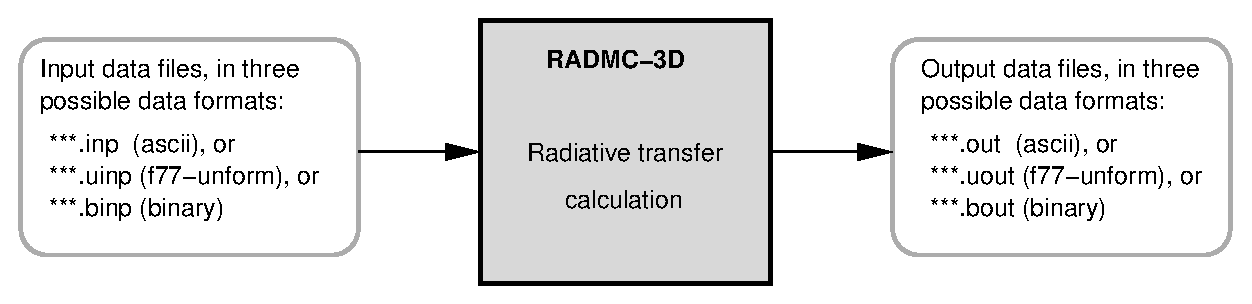
\includegraphics[height=0.13\textwidth]{dataflow_basic.eps}}
\caption{\label{fig-dataflow-basic}
Pictographic representation of the basic dataflow of RADMC-3D. The user
produces the input files; RADMC-3D reads them, performs the calculation,
and produces output files. The user can then analyze the output files.
}
\end{figure}
%
%
\begin{figure}
\centerline{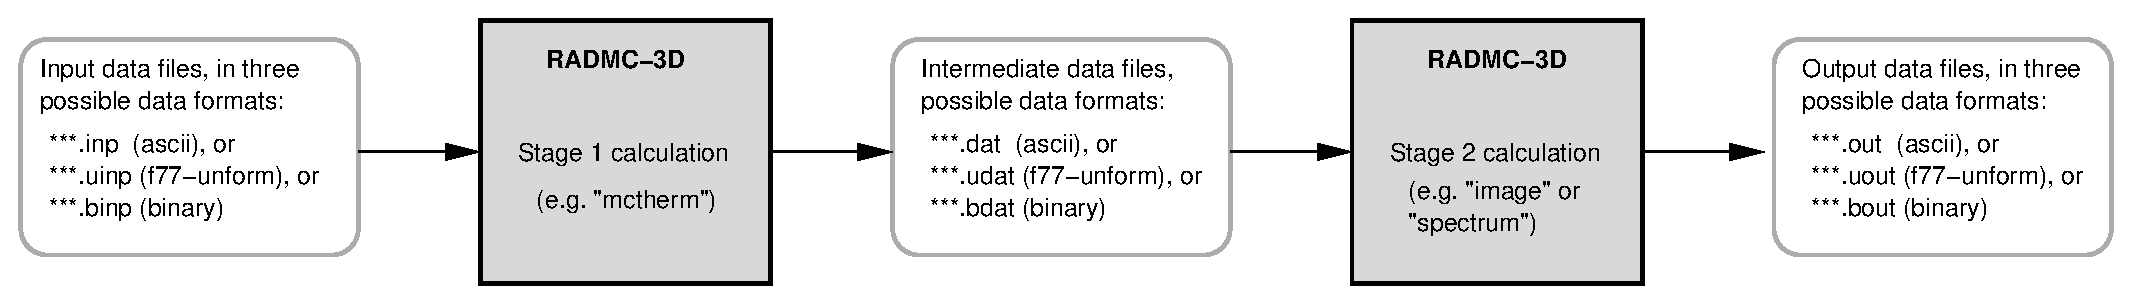
\includegraphics[height=0.13\textwidth]{dataflow_twostage.eps}}
\caption{\label{fig-dataflow-twostage}
Pictographic representation of the dataflow of RADMC-3D for the case
of a 2-stage procedure, such as for dust continuum transfer. An intermediate
file is produced that will be used by stage 2, but of course the user can
also analyze the intermediate file itself. 
}
\end{figure}
%
%
\begin{figure}
\centerline{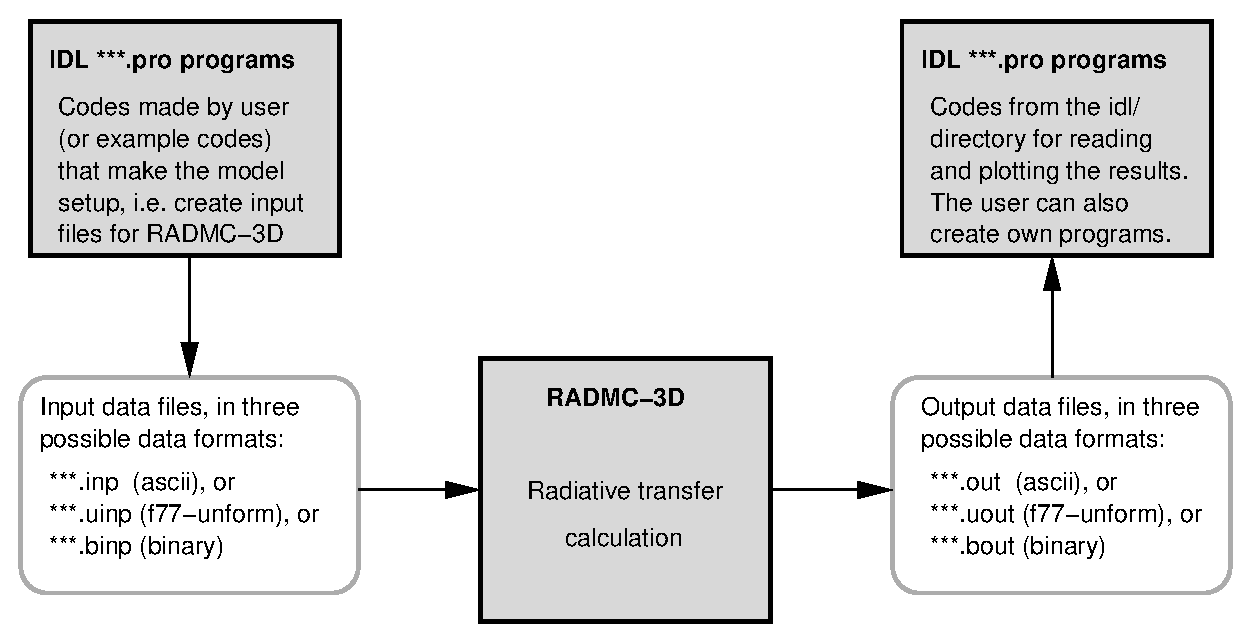
\includegraphics[height=0.28\textwidth]{dataflow_basic_idl.eps}}
\caption{\label{fig-dataflow-basic-idl}
Pictographic representation of how the IDL programs in the example directories
are used to create the input files of RADMC-3D. 
}
\end{figure}
%
%
\begin{figure}
\centerline{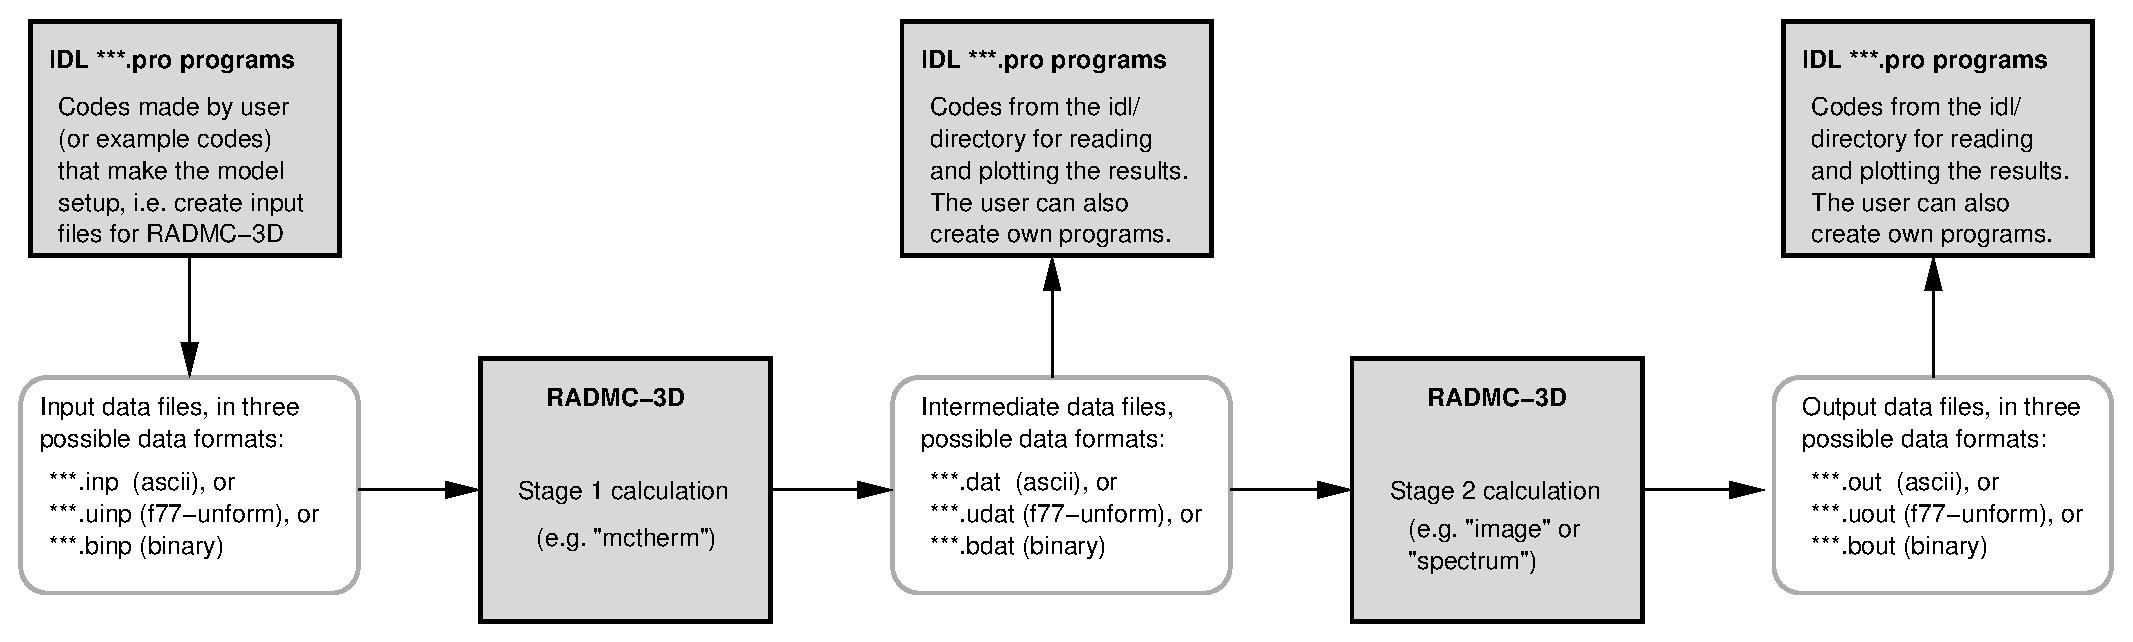
\includegraphics[height=0.28\textwidth]{dataflow_twostage_idl.eps}}
\caption{\label{fig-dataflow-twostage-idl}
Pictographic representation of the dataflow of RADMC-3D for the case
of a 2-stage procedure, such as for dust continuum transfer. An intermediate
file is produced that will be used by stage 2, but of course the user can
also analyze the intermediate file itself. 
}
\end{figure}
%

Several of these input files contain large tables, for instance of the
density at each grid point, or the stellar flux at each wavelength bin. It
is, of course, impossible to create these datafiles by hand. The idea is
that you design a program (in any language you like) that creates these
datafiles. In that program you essentially ``program the model''. We have
provided a number of example model setups in the {\small\tt examples/}
directory. For these examples models the setup programs were written in IDL
(their filenames all start with {\small\tt problem\_} and end with
{\small\tt .pro}). For you as the user it is therefore the easiest to start
from one of these examples and modify the IDL code to your needs. However,
if you have no IDL license, and/or if you prefer to use another language,
you can use the examples to see how the input files were generated and then
program this in another programming language.

{\em Note: The IDL files called {\small\tt problem\_***.pro} are meant to
be edited and changed by you! They are templates from which you can 
create your own models.} 

For the analysis of the output files created by RADMC-3D you can use your
own favorite plotting or data-analysis software. But also here we provide
some basic tools in IDL. These IDL routines are in the {\small\tt idl/}
directory. Typically you will create your own program, e.g.\ {\small\tt
  plot\_model.pro} or so, that will use these subroutines, e.g.\ by putting
in the first line: {\small\tt @readradmc.pro}. In this way IDL is used 
also as a post-processing tool. But again: this can also be done in another
language.

This procedure is shown in Fig.~\ref{fig-dataflow-basic-idl} for the
single-stage dataflow and in Fig.~\ref{fig-dataflow-twostage-idl} for the
two-stage dataflow.



\section{Radiative processes}
\label{sec-rad-processes}
%
Currently RADMC-3D handles the following radiative processes:
\begin{itemize}
\item {\em Dust thermal emission and absorption}\\
  RADMC-3D can compute spectra and images in dust continuum. The dust
  temperature must be known in addition to the dust density. In typical
  applications you will know the dust density distribution, but not the dust
  temperature, because the latter is the results of a balance between
  radiative absorption and re-emission. So in order to make spectra and
  images of a dusty object we must first calculate the dust temperature
  consistently. This can be done with RADMC-3D by making it perform a
  ``thermal Monte Carlo'' simulation (see Chapter \ref{chap-dust-transfer}).
  This can be a time-consuming computation. But once this is done, RADMC-3D
  writes the resulting dust temperatures out to the file {\small\tt
    dust\_temperature.dat}, which it can then later use for images and
  spectra. We can then call RADMC-3D again with the command to make an image
  or a spectrum (see Chapter \ref{chap-dust-transfer}). To summarize: a
  typical dust continuum radiative transfer calculation goes in two stages:
  \begin{enumerate}
  \item A thermal Monte Carlo simulation with RADMC-3D to compute the dust
    temperatures.
    \item A spectrum or image computation using ray-tracing with RADMC-3D.
  \end{enumerate}
\item {\em Dust scattering}\\
  Dust scattering is automatically included in the thermal Monte Carlo
  simulations described above, as well as in the production of images and
  spectra. For more details, consult Chapter \ref{chap-dust-transfer}.
\item {\em Gas atomic/molecular lines}\\
  RADMC-3D can compute spectra and images in gas lines (see Chapter
  \ref{chap-line-transfer}). The images are also known as ``channel
  maps''. To compute these, RADMC-3D must know the population densities of
  the various atomic/molecular levels. For now there are two options how to
  let RADMC-3D know these values:
  \begin{itemize}
  \item Tell RADMC-3D to assume that the molecules or atoms are in ``Local
    Thermodynamic Equilibrium'' (LTE), and specify the gas temperature at
    each location to allow RADMC-3D to compute these LTE level populations.
    {\em Note that in principle one is now faced with the same problem as
      with the dust continuum: we need to know the gas temperature, which we
      typically do not know in advance.} However, computing the gas
    temperature self-consistently is very difficult, because it involves
    many heating and cooling processes, some of which are very complex.
    That's why most line radiative transfer codes assume that the user gives
    the gas temperature as input. We do so as well. If you like, you can
    tell RADMC-3D to use the (previously calculated) dust temperature as the
    gas temperature, for convenience.
  \item Deliver RADMC-3D an input file with all the level populations
    that you have calculated youself using some method.
  \item Tell RADMC-3D to compute the level populations according to some
    simple local non-LTE prescription such as the Sobolev approximation
    (``Large Velocity Gradient method'') or the Escape Probability Method.
    (This is still under development!)
  \end{itemize}
  Currently RADMC-3D does not have a full non-local non-LTE computation
  method implemented. The reason is that it is very costly, and for many
  applications presumably not worth the computational effort. But we are
  working on a full non-LTE mode. Stay tuned!
\item {\em Gas continuum opacities}\\
  We are currently working on implementing gas continuum opacities as well.
  Again we are faced with the question how to compute the gas temperature.
  For now we simply require you to specify the gas temperature yourself.
\end{itemize}

{\em Remark:} We are thinking of methods to compute gas temperatures 
self-consistently in some special situations. Stay tuned...



\section{Coordinate systems}
\label{sec-coord-systems}
%
With RADMC-3D you can specify your density distribution in two 
coordinate systems:
\begin{itemize}
\item {\em Cartesian coordinates: 3-D}\\
  The simplest coordinate system is the Cartesian coordinate system
  $(x,y,z)$. For now each model must be 3-D (i.e.\ you must specify the
  densities and other quantities as a function of $x$, $y$ and $z$). 
\item {\em Cartesian coordinates: 1-D plane-parallel}\\
  This is like the normal cartesian coordinates, but now the $x$- and $y-$
  directions are ``infinitely extended''. Only the $z$-direction has
  finite-size cells, and hence the grid is only in $z$-direction.  This mode
  is the usual plane-parallel mode of radiative transfer.  See Section
  \ref{sec-1d-plane-parallel} for more details on this mode.
\item {\em Cartesian coordinates: 2-D pencil-parallel}\\
  This is the intermediate between full 3-D cartesian and 1-D
  plane-parallel.  In this mode only the $x$-direction is infinitely
  extended and a finite grid is in both $y$ and $z$ directions. This mode is
  only useful in very special cases, and is much less familiar to most - so
  use only when you are confident.
\item {\em Spherical coordinates}\\
  You can also specify your model in spherical coordinates
  $(r,\theta,\phi)$. These coordinates are related to the cartesian
  ones by:
  \begin{eqnarray}
    x &=& r \sin\theta \cos\phi \\
    y &=& r \sin\theta \sin\phi \\
    z &=& r \cos\theta
  \end{eqnarray}
  This means that the spatial variables (density, temperature etc) are all
  specified as a function of $(r,\theta,\phi)$. However, the location of the
  stars, the motion and direction of photon packages etc.~are still given in
  cartesian coordinates $(x,y,z)$. In other words: any function of space
  $f(\vec x)$ will be in spherical coordinates $f(r,\theta,\phi)$, but any
  point-like specification of position $\vec x$ will be given as Cartesian
  coordinates $\vec x=(x,y,z)$. This hybrid method allows us to do all
  physics in cartesian coordinates: photon packages or rays are treated
  always in cartesian coordinates, and so is the physics of scattering, line
  emission etc.  Only if RADMC-3D needs to know what the local conditions
  are (dust temperature, gas microturbulence, etc) RADMC-3D looks up which
  coordinates $(r,\theta,\phi)$ belong to the current $(x,y,z)$ and looks up
  the value of the density, microturbulence etc.\ at that location in the
  $(r,\theta,\phi)$ grid. And the same is true if RADMC-3D updates or
  calculates for instance the dust temperature: it will compute the
  $(r,\theta,\phi)$ belong to the current $(x,y,z)$ and update the
  temperature in the cell belonging to $(r,\theta,\phi)$. For the rest, all
  the physics is done in the Cartesian coordinate system. This has the major
  advantage that we do not need different physics modules for cartesian and
  spherical coordinates. Most parts of the code don't care which coordinate
  system is used: they will do their own work in Cartesian coordinates.
  When using spherical coordinates, please read Section
  \ref{sec-separable-refinement}.
\end{itemize}


\section{The spatial grid}
\label{sec-spatial-grid}
%
To specify the density or temperature structure (or any other spatial 
variable) as a function of spatial location we must have a grid. There
are two basic types of grids:
\begin{itemize}
\item {\em Structured grids (AMR grids)}\\
  The standard gridding is a simple rectangular grid. 
  \begin{itemize}
  \item {\em Cartesian coordinates:} When cartesian coordinates are used,
    this simply means that each cell is defined as $x_l<x<x_r$, $y_l<y<y_r$
    and $z_l<z<z_r$, where $l$ and $r$ stand for the left and right cell
    walls respectively. 
  \item {\em Spherical coordinates:} When spherical coordinates are used,
    this simply means that each cell is defined as $r_l<r<r_r$,
    $\theta_l<\theta<\theta_r$ and $\phi_l<\phi<\phi_r$.  Note therefore
    that the shape of the cells in spherical coordinates is (in real space)
    curved. For spherical coordinates the following four modes are
    available:
    \begin{itemize}
    \item {\em 1-D Spherical symmetry:} All spatial functions depend only on
      $r$.
    \item {\em 2-D Axial symmetry:} All spatial functions depend only on
      $r$ and $\theta$.
    \item {\em 2-D Axial symmetry with mirror symmetry:} All spatial
      functions depend only on $r$ and $\theta$, where the $\theta$ grid
      only covers the part above the $z=0$ plane. Internally it is in this
      mode assumed that all quantities below the $z=0$ plane are equal to
      those above the plane by mirror symmetry in the $z=0$ plane.  This
      saves a factor of two in computational effort for Monte Carlo
      calculations, as well as in memory useage. Note that also the
      resulting output files such as {\small\tt dust\_temperature.dat} will
      only be specified for $z>0$.
    \item {\em 3-D:} All spatial functions depend on all three variables
      $r$, $\theta$ and $\phi$.
    \item {\em 3-D with mirror symmetry:} All spatial functions depend on
      all three variables $r$, $\theta$ and $\phi$, but like in the 2-D
      case only the upper part of the model needs to be specified: the 
      lower part is assumed to be a mirror copy.
    \end{itemize}
    When using spherical coordinates, please read Section
    \ref{sec-separable-refinement}.
  \end{itemize}
  In all cases these structured grids allow for oct-tree-style grid
  refinement, or its simplified version: the layer-style grid
  refinement. See Section \ref{sec-grid-input} and Chapter
  \ref{chap-gridding} for more information about the gridding and the
  (adaptive) mesh refinement (AMR).
\item {\em Unstructured grids (for now: cartesian coordinates only)}\\
  For some applications it may be more convenient to specify spatial
  variables not on a structured grid, but on a semi-random set of points in
  3-D space. RADMC-3D will (hopefully) soon feature a mode in which it can
  handle such a situation, and use a Delaunay triangulation to produce a
  {\em triangulation} on the basis of this set of points, thus creating an
  {\em unstructured grid}. Unfortunately, for now this mode is not yet
  ready. Stay tuned...
\end{itemize}


\section{Computations that RADMC-3D can perform}
\label{sec-actions}
%
The code RADMC-3D (i.e.\ the executable {\small\tt radmc3d}) is {\em one}
code for {\em many} actions. Depending on which command-line arguments you
give, RADMC-3D can do various actions. Here is a list:
\begin{itemize}
\item {\em Compute the dust temperature:}\\
  With {\small\tt radmc3d mctherm} you call RADMC-3D with the command of
  performing a thermal Monte Carlo simulation to compute the dust temperature
  under the assumption that the dust is in radiative equilibrium with its
  radiation field. This is normally a prerequisite for computing SEDs and
  images from dusty objects (see ``computing spectra and images'' below).
  The output file of this computation is {\small\tt dust\_temperature.dat}
  which contains the dust temperature everywhere in the model.
\item {\em Compute a spectrum or SED:}\\
  With {\small\tt radmc3d sed} you call RADMC-3D with the command of
  performing a ray-tracing computation to compute the spectral energy
  distribution (SED) for the model at hand. Typically you first need to have
  called {\small\tt radmc3d mctherm} (see above) beforehand to compute dust
  temperatures (unless you have created the file {\small\tt
    dust\_temperature.dat} yourself because you have a special way of
  computing the dust temperature). With {\small\tt radmc3d sed} the spectrum
  is computed for the wavelengths points given in the file {\small\tt
    wavelength\_micron.inp}, which is the same wavelength grid that is used
  for {\small\tt radmc3d mctherm}. If you want to compute the spectrum at
  wavelength other than those used for the thermal Monte Carlo simulation,
  you should instead call {\small\tt radmc3d spectrum}, and you have the
  full freedom to choose the spectral wavelengths points at will, and you
  can specify these in various ways described in Section
  \ref{sec-set-camera-frequencies}.  Most easily you can create a file
  called {\small\tt camera\_wavelength\_micron.inp} (see Section
  \ref{sec-camera-wavelengths}) and call RADMC-3D using {\small\tt radmc3d
    spectrum loadlambda}. In all these cases the vantage point (where is the
  observer) can of course be set as well, see Section
  \ref{sec-dust-ray-tracing} and Chapter \ref{chap-images-spectra}.
\item {\em Compute an image:}\\
  With {\small\tt radmc3d image} you call RADMC-3D with the command of
  performing a ray-tracing computation to compute an image. You must specify
  the wavelength(s) at which you want the image by, for instance, calling
  RADMC-3D as {\small\tt radmc3d image lambda 10}, which makes the image at
  $\lambda=$10$\mu$m. But there are other ways by which the wavelength(s)
  can be set, see Section \ref{sec-set-camera-frequencies}.  In all these
  cases the vantage point (where is the observer) can of course be set as
  well, see Section \ref{sec-dust-ray-tracing} and Chapter
  \ref{chap-images-spectra}.
\item {\em Compute the local radiation field inside the model:}\\
  With {\small\tt radmc3d mcmono} you call RADMC-3D with the command of
  performing a wavelength-by-wavlength monochromatic Monte Carlo simulation
  (at the wavelengths that you specify in the file {\small\tt
    mcmono\_wavelength\_micron.inp}). The output file of this computation is
  {\small\tt mean\_intensity.out} which contains the mean intensity $J_\nu$
  as a function of the $(x,y,z)$ (cartesian) or $(r,\theta,\phi)$
  (spherical) coordinates at the frequencies $\nu_i\equiv 10^4c/\lambda_i$
  where $\lambda_i$ are the wavelengths (in $\mu$m) specified in the file
  {\small\tt mcmono\_wavelength\_micron.inp}. The results of this
  computation can be interesting for, for instance, models of
  photochemistry. But if you use RADMC-3D only for computing spectra and
  images, then you will not use this.
\end{itemize}
In addition to the above main methods, you can ask RADMC-3D to do various
minor things as well, which will be described throughout this manual.



\section{How a model is set up and computed: a rough overview}
A radiative transfer code such as RADMC-3D has the task of computing
synthetic images and spectra of a model that you specify. You tell the code
what the dust and/or gas density distribution in 3-D space is and where the
star(s) are, and the code will then tell you what your cloud looks like in
images and/or spectra. That's basically it. That's the main task of
RADMC-3D\footnote{It can/will, of course, do much more, but that is
described later in this manual.}.

First you have to tell RADMC-3D what 3-D distribution of dust and/or gas you
want it to model. For that you must specify a coordinate system (cartesian
or spherical) and a spatial grid. For cartesian coordinates this grid should
be 3-D (although there are exceptions to this), while for spherical
coordinates it can be 1-D (spherical symmetry), 2-D (axial symmetry) or 3-D
(no symmetry). RADMC-3D is (for most part) a cell-based code, i.e.\ your
grid devides space in cells and you have to tell RADMC-3D what the average
densities of dust and/or gas are in these cells.

The structure of the grid is specified in a file {\small\tt amr\_grid.inp}
(see Section \ref{sec-grid-input}). All the other data, such as dust density
and/or gas density are specified in other files, but all assume that the
grid is given by {\small\tt amr\_grid.inp}.

We can also specify the locations and properties of one or more stars in the
model. This is done in the {\small\tt stars.inp} (see Section
\ref{sec-stars}) file.

Now suppose we want to compute the appearance of our model in dust
continuum. We will describe this in detail in Chapter
\ref{chap-dust-transfer}, but let us give a very rough idea here. We write,
in addition to the {\small\tt amr\_grid.inp} and {\small\tt stars.inp}
files, a file {\small\tt dust\_density.inp} which specifies the density of
dust in each cell (see Section \ref{sec-dustdens}).  We also must write the
main input file {\small\tt radmc3d.inp} (see Section \ref{sec-radmc-inp}), but
we can leave it empty for now. We must give RADMC-3D a dust opacity table in
the files {\small\tt dustopac.inp} and for instance {\small\tt
  dustkappa\_silicate.inp} (see Section \ref{sec-opacities}). And finally, we
have to give RADMC-3D a table of discrete wavelengths in the file {\small\tt
  wavelength\_micron.inp} that it will use to perform its calculations
on. We then call the {\small\tt radmc3d} code with the keyword {\small\tt
  mctherm} (see Chapter \ref{chap-dust-transfer}) to tell it to perform a
Monte Carlo simulation to compute dust temperatures everywhere. RADMC-3D
will write this to the file {\small\tt dust\_temperature.dat}. If we now
want to make a spectral energy distribution, for instance, we call
{\small\tt radmc3d sed} (see Section \ref{sec-making-spectra}) and it will
write a file called {\small\tt spectrum.out} which is a list of fluxes at
the discrete wavelengths we specified in {\small\tt wavelength\_micron.inp}.
Then we are done: we have computed the spectral energy distribution of our
model. We could also make an image at wavelength 10 $\mu$m for instance with
{\small\tt radmc3d image lambda 10} (see Section \ref{sec-images}). This
will write out a file {\small\tt image.out} containing the image data
(see Section \ref{sec-image-out}).

As you see, RADMC-3D reads all its information from tables in various
files. Since you don't want to make large tables by hand, you will have
to write a little computer program that generates these tables automatically.
You can do this in any programming language you want. But in the example
models (see Section \ref{sec-example-models}) we use the programming 
language IDL (see Section \ref{sec-requirements}) for this. This is a
very simple (BASIC-like) programming language that makes it easy to
create the above input files. It is easiest to indeed have a look at
the example models to see how this is (or better: can be) done. 

We will explain all these things in much more detail below, and we will
discuss also many other radiative transfer problem types. The above example
is really just meant to give an impression of how RADMC-3D works. 



\section{Organization of model directories}
\label{sec-rough-overview-models}
%
The general philosophy of the RADMC-3D code package is the following. The
core of everything is the fortran code {\small\tt radmc3d}. This is the main
code which does the hard work for you: it makes the radiative transfer
calculations, makes images, makes spectra etc. Normally you compile this
code just once-and-for-all (see Chapter \ref{chap-compilation}), and then
simply use the executable {\small\tt radmc3d} for all models. There is an
exception to this `once-and-for-all' rule described in Section
\ref{sec-special-purpose-compile}, but in the present chapter we will not
use this (see Chapter \ref{chap-internal-setup} for this instead). So we
will stick here to the philosophy of compiling this code once and using it
for all models.

So how to set up a model? The trick is to present {\small\tt radmc3d} with a
set of input files in which the model is described in all its details. The
procedure to follow is this:
\begin{enumerate}
\item The best thing to do (to avoid a mess) is to make a directory for {\em
    each model}: one model, one directory. Since {\small\tt radmc3d} reads
  multiple input files, and also outputs a number of files, this is a good
  way to keep organized and we recommend it strongly.  So if we wish to make
  a new model, we make a new directory, or copy an old directory to a new
  name (if we merely want to make small changes to a prior model).
\item In this directory we generate the input files according to their
  required format (see Chapter \ref{chap-input-files}). You can create these
  input files in any way you want. But since many of these input files
  will/must contain huge lists of numbers (for instane, giving the density
  at each location in your model), you will typically want to write some
  script or program in some language (be it either C, C++, Fortran, IDL,
  GDL, perl, python, you name it) that automatically creates these input
  files. {\em We recommend using IDL, because we provide examples and
    standard subroutines in the programming language IDL; see below for more
    details. But IDL is not a strict requirement for using RADMC-3D.}
  Section \ref{sec-example-models} describes how to use the example IDL
  scripts to make these input files with IDL.
\item When all the input files are created, and we make sure that we are
  inside the model directory, we call {\small\tt radmc3d} with the desired
  command-line options (see Chapter \ref{chap-command-line-options}). This
  will do the work for us. 
\item Once this is done, we can analyze the results by reading the output
  files (see Chapter \ref{chap-input-files}). To help you reading and
  analyzing these output files you can use a set of IDL routines that we
  created for the user (see Chapter \ref{chap-idl-analysis-tools} and
  Section \ref{sec-install-idlscripts}). But here again, you are free to use
  any other plotting software and/or data postprocessing packages (many
  people favor python, for instance).
\end{enumerate}



\section{Running the example models}
\label{sec-example-models}
Often the fastest and easiest way to learn a code is simply to analyze and
run a set of example models. They are listed in the {\small\tt examples}
directory. Each model occupies a separate directory. This is also the style
we normally recommend: each model should have its own directory. Of course
there are also exceptions to this rule, and the user is free to organize
her/his data in any way he/she pleases. But in all the examples and
throughout this manual each model has its own directory.

To run an example model, go into the directory of this model, and follow the
directions that are written in the {\small\tt README} file in each of these
directories. {\em This is under the assumption that you have IDL installed on
your system, and that you have a license for it.}

Let us do for instance {\small\tt run\_simple\_1/}:
{\small\begin{verbatim}
cd examples/run_simple_1
\end{verbatim}}
Now we must create all the input files for this model. These input files are
all described in chapter \ref{chap-input-files}, but let us here just
'blindly' follow the example. In this example most (all except one) of the
input files are created using an IDL script called {\small\tt problem\_setup.pro}.
To execute this script, this is what you do:
{\small\begin{verbatim}
idl
IDL> .r problem_setup.pro 
IDL> exit
\end{verbatim}}
or in words: you go into IDL and {\em within the IDL prompt} you type {\small\tt
  .r problem\_setup.pro}, and if this is ready, you can leave IDL again (the
latter is not required of course)\footnote{Note that this does not work in IDL demo
  mode, which is what you get if you use IDL without a
  license, because files will be written, which is not possible in demo
  mode.}. This IDL script has now created a whole series
of input files, all ending with the extension {\small\tt .inp}. To see which
files are created, type the following in the shell: 
%
{\small\begin{verbatim}
ls -l *.inp
\end{verbatim}}

There is one file that this example does not create, and that is the file
{\small\tt dustkappa\_silicate.inp}. This is a file that contains the dust
opacity in tabulated form. This is a file that you as the user should
provide to the RADMC-3D code package. The file {\small\tt
  dustkappa\_silicate.inp} is merely an example, which is an
amorphous spherical silicate grain with radius 0.1 micron. But see
Section \ref{sec-opacities} for more information about the opacities.

Now that the input files are created we must run {\small\tt radmc3d}:
{\small\begin{verbatim}
radmc3d mctherm
\end{verbatim}}
This tells RADMC-3D to do the thermal Monte Carlo simulation. This may
take some time. When the model is ready, the prompt of the shell returns. 
To see what files have been created by this run of the code, type:
{\small\begin{verbatim}
ls -l *.dat
\end{verbatim}}
You will find the {\small\tt dust\_temperature.dat} containing the dust temperature
everywhere in the model. See again chapter \ref{chap-input-files} for
details of these files. To create a spectrum:
{\small\begin{verbatim}
radmc3d sed incl 45.
\end{verbatim}}
This will create a file {\small\tt spectrum.dat}.
To analyze these data you can use the IDL routines delivered with the code
(see Chapter \ref{chap-idl-analysis-tools} and Section \ref{sec-install-idlscripts}). 

There is a file {\small\tt Makefile} in the directory. This is here only
meant to make it easy to clean the directory. Type {\small\tt make
  cleanmodel} to clean all the output from the radmc3d code. Type {\small\tt
  make cleanall} to clean the directory back to basics.

Let us now do for instance model {\small\tt run\_simple\_1\_userdef/}:
{\small\begin{verbatim}
cd examples/run_simple_1_userdef
\end{verbatim}}
This is the same model as above, but now the grid and the dust density
are set up {\em inside} {\small\tt radmc3d}, using the file
{\small\tt userdef\_module.f90} which is present in this directory.
See Chapter \ref{chap-internal-setup} for details and follow the 
directions in the {\small\tt README} file. In short: first edit the
variable {\small\tt SRC} in the {\small\tt Makefile}  to point to the
{\small\tt src/} directory. Then type {\small\tt make}. Then go into
IDL and run the {\small\tt problem\_setup.pro} script (which now only
sets up the frequency grid, the star and the {\small\tt radmc3d.inp}
file and some small stuff). Now you can run the model. 

{\em Please read the README file in each of the example model directories.
Everything is explained there, including how to make the relevant plots.}







%----------------------------------------------------------------------------
%               CHAPTER: DUST CONTINUUM RADIATIVE TRANSFER
%----------------------------------------------------------------------------
\chapter{Dust continuum radiative transfer}
\label{chap-dust-transfer}
%
Many of the things related to dust continuum radiative transfer have
already been said in the previous chapters. But here we combine these
things, and expand with more in-depth information.

Most users simply want RADMC-3D to compute images and spectra from a
model. This is done in a two-stage procedure:
\begin{enumerate}
\item First compute the dust temperature everywhere using the thermal Monte
  Carlo computation (Section \ref{sec-dust-thermal-monte-carlo}).
\item Then making the images and/or spectra (Section \ref{sec-dust-ray-tracing}).
\end{enumerate}
You can then view the output spectra and images with the IDL tools or use
your own plotting software. 

Some expert users may wish to use RADMC-3D for something entirely different:
to compute the local radiation field {\em inside} a model, and use this
for e.g.\ computing photochemistry rates of a chemical model or so. 
This is described in Section \ref{sec-dust-monochromatic-monte-carlo}.

You may also use the thermal Monte Carlo computation of the dust temperature
to help estimating the {\em gas} temperature for the line radiative transfer.
See Chapter \ref{chap-line-transfer} for more on line transfer.



\section{The thermal Monte Carlo simulation: computing the dust temperature}
\label{sec-dust-thermal-monte-carlo}
%
RADMC-3D can compute the dust temperature using the Monte Carlo method of
Bjorkman \& Wood (2001, ApJ 554, 615) with various improvements such as the
continuous absorption method of Lucy (1999, A\&A 344, 282). Once a model is
entirely set up, you can ask {\small\tt radmc3d} to do the Monte Carlo
run for you by typing in a shell:
{\small\begin{verbatim}
radmc3d mctherm
\end{verbatim}}
if you use the standard {\small\tt radmc3d} code, or
{\small\begin{verbatim}
./radmc3d mctherm
\end{verbatim}}
if you have created a local version of {\small\tt radmc3d} 
(see Section \ref{sec-special-purpose-compile}).

What the method does is the following: First all the netto sources of energy
(or more accurately: sources of luminosity) are identified. The following
net sources of energy can be included:
\begin{itemize}
\item {\em Stars:} You can specify any number of individual stars: their
  position, and their spectrum and luminosity (See Section
  \ref{sec-stars}). This is the most commonly used source of luminosity, and
  as a beginning user we recommend to use only this for now.
\item {\em Continuum stellar source:} For simulations of galaxies it would
  require by far too many individual stars to properly include the input
  of stellar light from the billions of stars in the galaxy. To overcome
  this problem you can specify a continuously spatially distributed source
  of stars. {\em NOTE: Still in testing phase.}
\item {\em Viscous heating / internal heating:} Sometimes the dust grains
  acquire energy directly from the gas, for instance through viscous heating
  of the gas or adiabatic compression of the gas. This can be included as a
  spatially distributed source of energy. {\em NOTE: Still in
    progress... Not yet working.}
\end{itemize}
To compute the dust temperature we must have at least one source of
luminosity, otherwise the equilibrium dust temperature would be everywhere
0.

The next step is that this total luminosity is divided into {\small\tt
  nphot} packages, where {\small\tt nphot} is 100000 by default, but can be
set to any value by the user (see the file {\small\tt radmc3d.inp} described
in Section \ref{sec-radmc-inp}). Then these photon packages are emitted
by these sources one-by-one. As they move through the grid they may scatter
off dust grains and thus change their direction. They may also get absorbed
by the dust. If that happens, the photon package is immediately re-emitted
in another direction and with another wavelength. The wavelength is chosen
according to the recipe by Bjorkman \& Wood (2001, ApJ 554, 615). The
luminosity fraction that each photon package represents remains, however,
the same. Each time a photon package enters a cell it increases the
``energy'' of this cell and thus increases the temperature of the dust of
this cell.  The recipe for this is again described by Bjorkman \& Wood
(2001, ApJ 554, 615), but contrary to that paper we increase the temperature
of the dust always when a photon package enters a cell, while Bjorkman \&
Wood only increase the dust temperature if a discrete absorption event has
taken place. Each photon package will ping-pong through the model and never
gets lost until it escapes the model through the outer edge of the grid
(which, for cartesianl coordinates, is any of the grid edges in $x$, $y$ or
$z$, and for spherical coordinates is the outer edge of $r$). Once it
escapes, a new photon package is launched, until also it escapes. After all
photon packages have been launched and escaped, the dust temperature that
remains is the final answer of the dust temperature.

One must keep in mind that the temperature thus computed is an {\em
  equilibrium} dust temperature. It assumes that each dust grain acquires as
much energy as it radiates away. This is for most cases presumably a 
very good approximation, because the heating/cooling time scales for 
dust grains are typically very short compared to any time-dependent 
dynamics of the system. But there might be situations where this may not
be true: in case of rapid compression of gas, near shock waves or in 
extremely optically thick regions.

{\em NOTE:} Monte Carlo simulations are based on pseudo-random numbers.
The seed for the random number generator is by default set to -17933201.
If you want to perform multiple identical simulations with a different
random sequence you will need to set the seed by hand. This can be
done by adding a line 
{\small\begin{verbatim}
iseed = -5415
\end{verbatim}}
(where -5415 is to be replaced by the value you want) to the {\small\tt
  radmc3d.inp} file.

\subsection{Modified Random Walk method for high optical depths}
\label{sec-modrandwalk}
%
As you will soon find out: very optically thick models make the RADMC-3D
thermal Monte Carlo simulations to be slow. This is because in the thermal
Monte Carlo method a photon package is never destroyed unless it leaves the
system. A photon package can thus ``get lost'' deep inside an optically
thick region, making millions (or even billions) of absorption+reemission or
scattering events. Furthermore, you will notice that in order to get the
temperatures in these very optically thick regions to be reliable (i.e.\ not
too noisy) you may need a very large number of photon packages for your
simulation, which slows down the simulation even more. It is hard to prevent
such problems. Min, Dullemond, Dominik, de Koter \& Hovenier (2009) A\&A
497, 155 discuss two methods of dealing with this problem. One is a
diffusion method, which we will not discuss here. The other is the
``Modified Random Walk'' (MRW) method, based on the method by Fleck \&
Canfield (1984) J.Comput.Phys.\ 54, 508. Note that Robitaille (2010) A\&A
520, 70 presented a simplification of this method. Min et al.\ first
implemented this method into the MCMax code. Now, as of v.0.35, it is also
implemented in RADMC-3D, in Robitaille's simplified form.

The crucial idea of the method is that if a photon package ``gets lost''
deep inside a single ultra-optically-thick cell, we can use the analytical
solutions of the diffusion equation in a constant-density medium to predict
where the photon package will go next. This thus allows RADMC-3D to make a
single large step of the photon package which actually corresponds to
hundreds or thousands of absorption+reemission or scattering events.

The method works best if the optically thick cells are as large as possible.
This is because the analytical solutions are only valid within a single
cell, and thus the ``large step'' can not be larger than a single cell size.
Moreover, cell crossings will reduce the step length again to the physical
mean free path, so the more cell crossings are made, the less effective the
MRW becomes. 

{\em NOTE:} The MRW is by default switched off. The reason is that it is,
after all, an approximation. However, if RADMC-3D thinks that the MRW may
help speed up the thermal Monte Carlo, it will make the suggestion to the
user to switch on the MRW method. 

You can switch on the MRW by adding the following line to the
{\small\tt radmc3d.inp} file:
{\small\begin{verbatim}
modified_random_walk = 1
\end{verbatim}}

{\em NOTE:} This mode has only been added in version 0.34, so for now
stay vigilant when using it.



\section{Making SEDs, spectra, images for dust continuum}
\label{sec-dust-ray-tracing}
%
You can use RADMC-3D for computing spectra and images in dust continuum
emission. This is described in detail in Chapter
\ref{chap-images-spectra}. RADMC-3D needs to know not only the dust spatial
distribution, given in the file {\small\tt dust\_density.inp}, but also the
dust temperature, given in the file {\small\tt dust\_temperature.dat} (see
Chapter \ref{chap-binary-io} for the binary version of these files, which
are more compact, and which you can use instead of the ascii versions). The
{\small\tt dust\_temperature.dat} is normally computed by RADMC-3D itself
through the thermal Monte Carlo computation (see Section
\ref{sec-dust-thermal-monte-carlo}). But if you, the user, wants to specify
the dust temperature at each location in the model youself, then you can
simply create your own file {\small\tt dust\_temperature.dat} and skip the
thermal Monte Carlo simulation and go straight to the creation of images or
spectra.

The basic command to make a spectrum at the global grid of wavelength
(specified in the file {\small\tt wavelength\_micron.inp},
see Section \ref{sec-wavelengths}) is:
{\small\begin{verbatim}
radmc3d sed
\end{verbatim}}
You can specify the direction of the observer with {\small\tt incl}
and {\small\tt phi}:
{\small\begin{verbatim}
radmc3d sed incl 20 phi 80
\end{verbatim}}
which means: put the observer at inclination 20 degrees and $\phi$-angle
80 degrees.

You can also make a spectrum for a given grid of wavelength (independent
of the global wavelength grid). You first create a file
{\small\tt camera\_wavelength\_micron.inp}, which has the same format
as {\small\tt wavelength\_micron.inp}. You can put any set of wavelengths
in this file without modifying the global wavelength grid (which is used
by the thermal Monte Carlo computation). Then you type
{\small\begin{verbatim}
radmc3d spectrum loadlambda
\end{verbatim}}
and it will create the spectrum on this wavelength grid. More information
about making spectra is given in Chapter \ref{chap-images-spectra}.

For creating an image you can type
{\small\begin{verbatim}
radmc3d image lambda 10
\end{verbatim}}
which creates an image at wavelength $\lambda$=10$\mu$m. More information
about making images is given in Chapter \ref{chap-images-spectra}.

{\em Important note:} To handle scattering of light off dust grains, the
ray-tracing is preceded by a quick Monte Carlo run that is specially
designed to compute the ``scattering source function''. This Monte Carlo
run is usually {\em much} faster than the thermal Monte Carlo run, but must
be done at each wavelength. It can lead, however, to slight spectral noise,
because the random photon paths are different for each wavelength. 
See Section \ref{sec-scattering} for details.

\section{OpenMP parallelized Monte Carlo}
\label{sec-omp-mc}
%
Depending on the model properties and the number of photon packages used in
the simulation the Monte Carlo calculation (in particular the thermal Monte
Carlo, but under some conditions also the scattering Monte Carlo) can be a
time-consuming computation when executed only in a serial mode. To improve
this, these Monte Carlo calculations can be done in OpenMP parallel mode.
The loop over photon packages is then distributed amongst the different
threads, where each thread adopts a specific number of loop iterations
following the order of the thread identification number. To this end the
random number generator was modified. The important point for the parallel
version is that different threads must not share the same random seed
initially. To be certain that each thread is assigned a different seed at
the beginning, the thread identity number is added to the initial seed.

The default value for the number of threads in the parallel version is set
to one, so that the program is identical with the serial version, except for
the random generator's initial seed. The user can change the value by either
typing `setthreads’ and a number of threads (integer value) in the command
line or by adding a corresponding line to the {\small\tt radmc3d.inp}
file. If the chosen number of threads is larger than the available number of
processor cores, the user is asked to reduce it.

For example, you can ask {\small\tt radmc3d} to do the parallelized Monte
Carlo run for you by typing in a shell:
{\small\begin{verbatim}
radmc3d mctherm setthreads 4
\end{verbatim}}
or by adding the following keyword to the {\small\tt radmc3d.inp} file:
{\small\begin{verbatim}
setthreads = 4
\end{verbatim}}
which means that four threads are used for the thermal Monte Carlo
computation.

For the image or spectrum you can do the same: just add {\small\tt 
setthreads 4} or so on the command line or put {\small\tt 
setthreads = 4} into the {\small\tt radmc3d.inp} file.

Make sure that you have included the {\small\tt -fopenmp} keyword in the
{\small\tt Makefile} and have compiled the whole {\small\tt radmc3d} source
code with this additional command before using the OpenMP parallelized
thermal Monte Carlo version (cf.\ Sect.\ \ref{sec-makeing}).


\section{Overview of input data for dust radiative transfer}
%
In order to perform any of the actions described in Sections
\ref{sec-dust-thermal-monte-carlo}, \ref{sec-dust-monochromatic-monte-carlo}
or \ref{sec-dust-ray-tracing}, you must give RADMC-3D the following 
data:
\begin{itemize}
\item {\small\tt amr\_grid.inp:} The grid file (see Section
  \ref{sec-grid-input}).
\item {\small\tt wavelength\_micron.inp:} The global wavelength file (see
  Section \ref{sec-wavelengths}).
\item {\small\tt stars.inp:} The locations and properties of stars (see
  Section \ref{sec-stars}).
\item {\small\tt dust\_density.inp:} The spatial distribution of dust
  on the grid (see Section \ref{sec-dustdens}).
\item {\small\tt dustopac.inp:} A file with overall information about
  the various species of dust in the model (see Section \ref{sec-opacities}).
  One of the main pieces of information here is (a) how many dust species
  are included in the model and (b) the tag names of these dust species
  (see {\small\tt dustkappa\_XXX.inp} below). The file 
  {\small\tt dust\_density.inp} must contain exactly this number of
  density distributions: one density distribution for each dust species.
\item {\small\tt dustkappa\_XXX.inp:} One or more dust opacity files (where
  {\small\tt XXX} should in fact be a tag name you define, for instance
  {\small\tt dustkappa\_silicate.inp}). The labels are listed in the
  {\small\tt dustopac.inp} file. ee Section \ref{sec-opacities} for more
  information.
\item {\small\tt camera\_wavelength\_micron.inp (optional):} This file is
  only needed if you want to create a spectrum at a special set of
  wavelengths (otherwise use {\small\tt radmc3d sed}).
\item {\small\tt mcmono\_wavelength\_micron.inp (optional):} This file is
  only needed if you want to compute the radiation field inside the model by
  calling {\small\tt radmc3d mcmono} (e.g.\ for photochemistry).
\end{itemize}
Other input files could be required in certain cases, but you will then
be asked about it by RADMC-3D.



\section{Special-purpose feature: Computing the local radiation field}
\label{sec-dust-monochromatic-monte-carlo}
%
If you wish to use RADMC-3D for computing the radiation field {\em inside}
the model, for instance for computing photochemical rates in a chemical model,
then RADMC-3D can do so by calling RADMC-3D in the following way:
{\small\begin{verbatim}
radmc3d mcmono
\end{verbatim}}
This computes the mean intensity 
\begin{equation}
  J_\nu = \frac{1}{4\pi}\oint I_\nu(\Omega)d\Omega
\end{equation}
(in units of erg$\,$s$^{-1}$$\,$cm$^{-2}$$\,$Hz$^{-1}$$\,$ster$^{-1}$) as a
function of the $(x,y,z)$ (cartesian) or $(r,\theta,\phi)$ (spherical)
coordinates at frequencies $\nu_i\equiv 10^4c/\lambda_i$ where $\lambda_i$
are the wavelengths (in $\mu$m) specified in the file {\small\tt
  mcmono\_wavelength\_micron.inp} (same format as the file {\small\tt
  wavelength\_micron.inp} which is described in Section
\ref{sec-wavelengths}). The results of this computation can be interesting
for, for instance, models of photochemistry.

The file that is produced by {\small\tt radmc3d mcmono} is called
{\small\tt mean\_intensity.out} and has the following form:
\begin{asciibox}\begin{verbatim}
iformat                                  <=== Typically 2 at present
nrcells
nfreq                                    <=== Nr of frequencies 
freq_1 freq_2 ... freq_nfreq             <=== List of frequencies in Hz
meanint[1,icell=1]
meanint[1,icell=2]
...
meanint[1,icell=nrcells]
meanint[2,icell=1]
meanint[2,icell=2]
...
meanint[2,icell=nrcells]
...
...
...
meanint[nfreq,icell=1]
meanint[nfreq,icell=2]
...
meanint[nfreq,icell=nrcells]
\end{verbatim}\end{asciibox}
The list of frequencies will, in fact, be the same as those listed in the
file {\small\tt mcmono\_wavelength\_micron.inp}.

Note that if your model is very large, the computation of the radiation
field on a large set of wavelength could easily overload the memory of the
computer. However, often you are in the end not interested in the entire
spectrum at each location, but just in integrals of this spectrum over some
cross section. For instance, if you want to compute the degree to which dust
shields molecular photodissociation lines in the UV, then you only need to
compute the total photodissociation rate, which is an integral of the
photodissociation cross section times the radiation field. In Section
\ref{sec-compute-radiation-integrals} it will be explained how you can
create a userdef subroutine (see Chapter \ref{chap-internal-setup}) that
will do this for you in a memory-saving way.

There is an important parameter for this Monochromatic Monte Carlo that you
may wish to play with:
\begin{itemize}
\item {\small\tt nphot\_mono}\\
  The parameter {\small\tt nphot\_mono} sets the number of photon packages
  that are used for the Monochromatic Monte Carlo simulation. It has as
  default 100000, but that may be too little for 3-D models. You can set
  this value in two ways:
  \begin{itemize}
    \item In the {\small\tt radmc3d.inp} file as a line {\small\tt nphot\_mono =}
      {\small\tt 1000000} for instance.
    \item On the command-line by adding {\small\tt nphot\_mono} {\small\tt 
        1000000}. 
  \end{itemize}
\end{itemize}




\section{More about scattering of photons off dust grains}
\label{sec-scattering}
%
Photons can not only be absorbed and re-emitted by dust grains: They can
also be scattered. Scattering does nothing else than change the direction of
propagation of a photon, and in case polarization is included, its Stokes
parameters. Strictly speaking it may also slightly change its wavelength, if
the dust grains move with considerable speed they may Doppler-shift the
wavelength of the outgoing photon (which may be relevant, if at all, when
dust radiative transfer is combined with line radiative transfer, see
chapter \ref{chap-line-transfer}), but this subtle effect is not treated in
RADMC-3D. For RADMC-3D scattering is just the changing of direction of a
photon.

\subsection{Five modes of treating scattering}
\label{sec-modes-of-scattering}
%
RADMC-3D has five levels of realism of treatment of scattering, starting
with {\small\tt scattering\_mode=1} (simplest) to {\small\tt
  scattering\_mode=5} (most realistic):
\begin{enumerate}
\item {\em No scattering ({\small\tt scattering\_mode=0}):}\\
  If either the {\small\tt dustkappa\_XXX.inp} files do not contain a
  scattering opacity or scattering is switched off by setting {\small\tt
    scattering\_mode\_max} to 0 in the {\small\tt radmc3d.inp} file, then
  scattering is ignored. It is then assumed that the dust grains have zero
  albedo.
\item {\em Isotropic scattering ({\small\tt scattering\_mode=1}):}\\
  If either the {\small\tt dustkappa\_XXX.inp} files do not contain
  information about the anisotropy of the scattering or anisotropic
  scattering is switched off by setting {\small\tt scattering\_mode\_max} to
  1 in the {\small\tt radmc3d.inp} file, then scattering is treated as
  isotropic scattering.  Note that this can be a bad approximation.
\item {\em Anisotropic scattering using Henyey-Greenstein ({\small\tt scattering\_mode=2}):}\\
  If the {\small\tt dustkappa\_XXX.inp} files contain the scattering opacity
  and the $g$ parameter of anisotropy (the Henyey-Greenstein $g$ parameter
  which is equal, by definition, to $g=\langle\cos\theta\rangle$, where
  $\theta$ is the scattering deflection angle), and {\small\tt
    scattering\_mode\_max} is set to 2 or higher in the {\small\tt
    radmc3d.inp} file then anisotropic scattering is treated using the
  Henyey-Greenstein approximate formula.
\item {\em Anisotropic scattering using tabulated phase function ({\small\tt scattering\_mode=3}):}\\
  To treat scattering using a tabulated phase function, you must specify the
  dust opacities using {\small\tt dustkapscatmat\_XXX.inp} files instead of the
  simpler {\small\tt dustkappa\_XXX.inp} files (see 
  Section \ref{sec-dustkapscatmat-files}). You must also set {\small\tt
    scattering\_mode\_max} is set to 3 or higher.
\item {\em Anisotropic scattering with polarization for last scattering ({\small\tt scattering\_mode=4}):}\\
  To treat scattering off randomly oriented particles with the full
  polarization you need to set {\small\tt scattering\_mode\_max} is set to 4
  or higher, and you must specify the full dust opacity and scattering
  matrix using the {\small\tt dustkapscatmat\_XXX.inp} files instead of the
  simpler {\small\tt dustkappa\_XXX.inp} files (see Section
  \ref{sec-dustkapscatmat-files}). If {\small\tt scattering\_mode=4} the
  full polarization is only done upon the last scattering before light
  reaches the observer (i.e.\ it is only treated in the computation of
  the scattering source function that is used for the images, but it is
  not used for the movement of the photons in the Monte Carlo simulation).
  See Section \ref{sec-polarized-scattering} for more information about
  polarized scattering.
\item {\em Anisotropic scattering with polarization, full treatment ({\small\tt scattering\_mode=5}):}\\
  For the full treatment of polarized scattering off randomly oriented
  particles, you need to set {\small\tt scattering\_mode\_max} is set to 5,
  and you must specify the full dust opacity and scattering matrix using the
  {\small\tt dustkapscatmat\_XXX.inp} files instead of the simpler {\small\tt
    dustkappa\_XXX.inp} files (see Section \ref{sec-dustkapscatmat-files}).
  See Section \ref{sec-polarized-scattering} for more information about
  polarized scattering.
\end{enumerate}
Please refer to Sections \ref{sec-scat-phasefunc} and
\ref{sec-polarized-scattering} for more information about these different
scattering modes.

So in summary: the dust opacity files themselves tell how detailed the
scattering is going to be included. If no scattering information is present
in these files, RADMC-3D has no choice but to ignore scattering. If they
only contain scattering opacities but no phase information (no $g$-factor),
then RADMC-3D will treat scattering in the isotropic approximation. If 
the $g$-factor is also included, then RADMC-3D will use the Henyey-Greenstein
formula for anisotropic scattering. If you specify the full scattering
matrix (using the {\small\tt dustkapscatmat\_XXX.inp} files instead of
the {\small\tt dustkappa\_XXX.inp} files) then you can use tabulated
scattering phase functions, and even polarized scattering. 

If {\small\tt scattering\_mode\_max} is {\em not} set in the {\small\tt
radmc3d.inp} file, it is by default 9999, meaning: RADMC-3D will always
use the maximally realistic scattering mode that the dust opacities
allow.

BUT you can always limit the realism of scattering by setting the {\small\tt
  scattering\_mode\_max} to 4, 3, 3, 1 or 0 in the file {\small\tt
  radmc3d.inp}. This can be useful to speed up the calculations or be sure
to avoid certain complexities of the full phase-function treatment of
scattering.

At the moment there are some limitations to the full anisotropic scattering
treatment:
\begin{itemize}
\item {\em Anisotropic scattering in 1-D and 2-D Spherical coordinates:}\\
  For 1-D and 2-D Spherical coordinates there is currently no possibility of
  treating anisotropic scattering in the image- and spectrum-making.  The
  reason is that the scattering source function (see Section
  \ref{sec-scat-monte-carlo}) must be stored in an angle-dependent
  way. However, in 2-D spherical coordinates, each cell is in fact a ring
  around the symmetry axis, and the angular dependence of the scattering
  source function would depend on which position along the ring the
  scattering takes place (with respect to the location of the observer).
  {\em This will be fixed hopefully later by storing the scattering source
    function for different angles in each cell; stay tuned!}
\item {\em Full phase functions and polarization only for randomly-oriented particles:}\\
  Currently RADMC-3D cannot handle scattering off fixed-oriented
  non-spherical particles, because it requires a much more detailed handling
  of the angles. It would require at least 3 scattering angles (for
  axially-symmetric particles) or more (for completely asymmetric
  particles), which is currently beyond the scope of RADMC-3D.
\end{itemize}

\subsection{Scattering phase functions}
\label{sec-scat-phasefunc}
%
As mentioned above, for the different {\small\tt scattering\_mode} settings
you have different levels of realism of treating scattering. 

The transfer equation along each ray, ignoring polarization for now, is:
\begin{equation}
\label{eq-ray-tracing-rt}
\frac{dI_\nu}{ds} = j_\nu^{\mathrm{therm}} + j_\nu^{\mathrm{scat}} 
- (\alpha_\nu^{\mathrm{abs}}+\alpha_\nu^{\mathrm{scat}}) I_\nu
\end{equation}
where $\alpha_\nu^{\mathrm{abs}}$ and $\alpha_\nu^{\mathrm{scat}}$ are the
extinction coefficients for absorption and scattering.  Let us assume, for
convenience of notation, that we have just one dust species with density
dstribution $\rho$, absorption opacity $\kappa_\nu^{\mathrm{abs}}$ and
scattering opacity $\kappa_\nu^{\mathrm{scat}}$. We then have
\begin{eqnarray}
\alpha_\nu^{\mathrm{abs}} &\equiv& \rho\kappa_\nu^{\mathrm{abs}}\\
\alpha_\nu^{\mathrm{scat}} &\equiv& \rho\kappa_\nu^{\mathrm{scat}}\\
j_\nu^{\mathrm{therm}} &=& \alpha_\nu^{\mathrm{abs}} B_\nu(T)\label{eq-thermal-source-function}
\end{eqnarray}
where $B_\nu(T)$ is the Planck function. The last equation is an expression
of Kirchhoff's law. 

For {\em isotropic} scattering ({\small\tt scattering\_mode}=1) the
scattering source function $j_\nu^{\mathrm{scat}}$ is given by
\begin{eqnarray}
j_\nu^{\mathrm{scat}} = \alpha_\nu^{\mathrm{scat}} \frac{1}{4\pi}\oint I_\nu d\Omega
\end{eqnarray}
where the integral is the integral over solid angle. In this case
$j_\nu^{\mathrm{scat}}$ does not depend on solid angle. 

For {\em anisotropic} scattering ({\small\tt scattering\_mode}$\ge$2) we
must introduce the scattering phase function $\Phi({\bf n}_{\mathrm{in}},
{\bf n}_{\mathrm{out}})$, where
${\bf n}_{\mathrm{in}}$ is the unit direction vector for incoming radiation
and ${\bf n}_{\mathrm{out}}$ is the unit direction vector for the scattered
radiation. The 
scattering phase function is normalized to unity:
\begin{equation}
\frac{1}{4\pi}\oint\Phi({\bf n}_{\mathrm{in}},
{\bf n}_{\mathrm{out}}) d\Omega_{\mathrm{out}}
=\frac{1}{4\pi}\oint\Phi({\bf n}_{\mathrm{in}},
{\bf n}_{\mathrm{out}}) d\Omega_{\mathrm{in}}=1
\end{equation}
where we integrated over all possible ${\bf n}_{\mathrm{out}}$ or
${\bf n}_{\mathrm{in}}$.
Then the scattering source function becomes:
\begin{eqnarray}
j_\nu^{\mathrm{scat}}({\bf n}_{\mathrm{out}}) = 
\alpha_\nu^{\mathrm{scat}} \frac{1}{4\pi}\oint I_\nu({\bf n}_{\mathrm{in}})
\Phi({\bf n}_{\mathrm{in}},{\bf n}_{\mathrm{out}}) d\Omega_{\mathrm{in}}
\end{eqnarray}
which is angle-dependent. The angular dependence means: a photon package has
not completely forgotten from which direction it came before hitting the
dust grain. 

If we do not include the polarization of radiation and we have randomly
oriented particles, then the scattering phase function will only depend
on the scattering (deflection) angle $\theta$ defined by
\begin{equation}
\cos\theta \equiv \mu = {\bf n}_{\mathrm{out}}\cdot {\bf n}_{\mathrm{in}}
\end{equation}
We will thus be able to write
\begin{equation}
\Phi({\bf n}_{\mathrm{in}},{\bf n}_{\mathrm{out}})
\equiv \Phi(\mu)
\end{equation}
where $\Phi(\mu)$ is normalized as
\begin{equation}
\frac{1}{2}\int_{-1}^{+1} \Phi(\mu) d\mu = 1
\end{equation}

If we have {\small\tt scattering\_mode}=2 then the phase function is
the Henyey-Greenstein phase function defined as
\begin{equation}
\Phi(\mu)=\frac{1-g^2}{(1+g^2-2g\mu)^{3/2}}
\end{equation}
where the value of the anisotropy parameter $g$ is taken from the
dust opacity file. Note that for $g=0$ you get $\Phi(\mu)=1$ which is
the phase function for isotropic scattering.

If we have {\small\tt scattering\_mode}=3 then the phase function is
tabulated by you. You have to provide the tabulated phase function as the
$Z_{11}(\theta)$ scattering matrix element for a tabulated set of $\theta_i$
values, and this is done in a file {\small\tt dustkapscatmat\_xxx.inp} (see
Section \ref{sec-dustkapscatmat-files} and note that for {\small\tt
  scattering\_mode}=3 the other $Z_{ij}$ elements can be kept 0 as they are
of no consequence). The relation between $Z_{11}(\theta)$ and 
$\Phi(\mu)$ is:
\begin{equation}
\Phi(\mu) \equiv \Phi(\cos(\theta)) = \frac{4\pi}{\kappa_{\mathrm{scat}}}\,Z_{11}(\theta)
\end{equation}
(which holds at each wavelength individually).

If we have {\small\tt scattering\_mode}=4 then the scattering in the Monte
Carlo code is done according to the tabulated $\Phi(\mu)$ mode mentioned
above, but for computing the scattering source function the full polarized
scattering matrix is used. See Section \ref{sec-polarized-scattering}.

If we have {\small\tt scattering\_mode}=5 then the scattering phase
function is not only dependent on $\mu$ but also on the other angle.
And it depends on the polarization state of the input radiation. See 
Section \ref{sec-polarized-scattering}.


\subsection{Scattering of photons in the Thermal Monte Carlo run}
\label{sec-scat-in-therm-mc}
%
So how is scattering treated in practice? In the thermal Monte Carlo model
(Section \ref{sec-dust-thermal-monte-carlo}) the scattering has only one
effect: it changes the direction of propagation of the photon packages
whenever such a photon package experiences a scattering event. This may
change the results for the dust temperatures subtly. In special cases it may
even change the dust temperatures more strongly, for instance if scattering
allows ``hot'' photons to reach regions that would have otherwise been in
the shadow. It may also increase the optical depth of an object and thus
change the temperatures accordingly. But this is all there is to it.

If you include the full treatment of polarized scattering ({\small\tt
  scattering\_mode=5}), then a photon package also gets polarized when it
undergoes a scattering event. This can affect the phase function for the
next scattering event. This means that the inclusion of the full polarized
scattering processes (as opposed to using non-polarized photon packages)
can, at least in principle, have an effect on the dust temperatures that
result from the thermal Monte Carlo computation. This effect is, however,
rather small in practice. 


\subsection{Scattering of photons in the Monochromatic Monte Carlo run}
\label{sec-scat-in-mono-mc}
%
For the monochromatic Monte Carlo calculation for computing the mean
intensity radiation field (Section \ref{sec-dust-monochromatic-monte-carlo})
the scattering has the same effect as for the thermal Monte Carlo model: it
changes the direction of photon packages. In this way ``hot'' radiation may
enter regions which would otherwise have been in a shadow. And by increasing
the optical depth of regions, it may increase the local radiation field by
the greenhouse effect or decrease it by preventing photons from entering
it. As in the thermal Monte Carlo model the effect of scattering in the
monochromatic Monte Carlo model is simply to change the direction of motion
of the radiation field, but for the rest nothing differs to the case without
scattering. Also here the small effects caused by polarized scattering apply,
like in the thermal Monte Carlo case.

\subsection{Scattered light in images and spectra: The ``Scattering Monte Carlo'' computation}
\label{sec-scat-monte-carlo}
%
For making images and spectra with the ray-tracing capabilities of RADMC-3D
(see Section \ref{sec-dust-ray-tracing} and Chapter
\ref{chap-images-spectra}) the role of scattering is a much more complex one
than in the thermal and monochromatic Monte Carlo runs. The reason is that
the scattered radiation will eventually end up on your images and spectra.

If we want to make an image or a spectrum, then for each pixel we must
integrate Eq.~(\ref{eq-ray-tracing-rt}) along the 1-D ray belonging to that
pixel. If we performed the thermal Monte Carlo simulation beforehand (or if
we specified the dust temperatures by hand) we know the thermal source
function through Eq.~(\ref{eq-thermal-source-function}). But we have, at
that point, no information yet about the scattering source function. The
thermal Monte Carlo calculation {\em could} have also stored this function
at each spatial point and each wavelength and each observer direction, but
that would require gigantic amounts of memory (for a typical 3-D model it
might be many Gbytes, going into the Tbyte regime). So in RADMC-3D the
scattering source function is {\em not} computed during the thermal
Monte Carlo run. 

In RADMC-3D the scattering source function $j_\nu^{\mathrm{scat}}(\Omega')$
is computed {\em just prior to} the ray-tracing through a brief ``Scattering
Monte Carlo'' run. This is done {\em automatically} by RADMC-3D, so you
don't have to worry about this. Whenever you ask RADMC-3D to make an image
(and if the scattering is in fact included in the model, see Section
\ref{sec-modes-of-scattering}), RADMC-3D will automatically realize that it
requires knowledge of $j_\nu^{\mathrm{scat}}(\Omega')$, and it will start a
brief single-wavelength Monte Carlo simulation for computing
$j_\nu^{\mathrm{scat}}(\Omega')$. This single-wavelength ``Scattering Monte
Carlo'' simulation is relatively fast compared to the thermal Monte Carlo
simulation, because photon packages can be destroyed by absorption. So
photon packages do not bounce around for long, as they do in the thermal
Monte Carlo simulation.  This Scattering Monte Carlo simulation is in fact
very similar to the monochromatic Monte Carlo model described in Section
\ref{sec-dust-monochromatic-monte-carlo}. While the monochromatic Monte
Carlo model is called specifically by the user (by calling RADMC-3D with
{\small\tt radmc3d mcmono}), the Scattering Monte Carlo simulation is not
something the user must specify him/her-self: it is automatically done by
RADMC-3D if it is needed (which is typically before making an image or
during the making of a spectrum). And while the monochromatic Monte Carlo
model returns the mean intensity inside the model, the Scattering Monte Carlo
simulation provides the raytracing routines with the scattering source
function but does {\em not} store this function in a file.

You can see this happen if you have a model with scattering opacity
included, and you make an image with RADMC-3D, you see that it prints
{\small\tt 1000}, {\small\tt 2000}, {\small\tt 3000}, ... etc., in other
words, it performs a little Monte Carlo simulation before making the
image.

There is an important parameter for this Scattering Monte Carlo that you
may wish to play with:
\begin{itemize}
\item {\small\tt nphot\_scat}\\
  The parameter {\small\tt nphot\_scat} sets the number of photon packages
  that are used for the Scattering Monte Carlo simulation. It has as default
  100000, but that may be too little for 3-D models and/or cases where you
  wish to reduce the ``streaky'' features sometimes visible in
  scattered-light images when too few photon packages are used. You can
  set this value in two ways:
  \begin{itemize}
    \item In the {\small\tt radmc3d.inp} file as a line {\small\tt nphot\_scat =}
      {\small\tt 1000000} for instance.
    \item On the command-line by adding {\small\tt nphot\_scat} {\small\tt 
        1000000}. 
  \end{itemize}
  In Figure \ref{fig-polscat} you can see how the quality of an image in 
  scattered light improves when increasing {\small\tt nphot\_scat}.
\item {\small\tt nphot\_spec}\\
  The parameter {\small\tt nphot\_spec} is actually exactly the same as
  {\small\tt nphot\_scat}, but is used (and used only!) for the creation of
  spectra. The default is 10000, i.e.~substantially smaller than {\small\tt
    nphot\_scat}. The reason for this separate parameter is that if you make
  spectra, you integrate over the image to obtain the flux (i.e.~the value of
  the spectrum at that wavelength). Even if the scattered light image may
  look streaky, the integral may still be accurate. We can thus afford much
  fewer photon packages when we make spectra than when we make images, and
  can thus speed up the calculation of the spectrum. You can set this value
  in two ways:
  \begin{itemize}
    \item In the {\small\tt radmc3d.inp} file as a line {\small\tt nphot\_spec =}
      {\small\tt 100000} for instance.
    \item On the command-line by adding {\small\tt nphot\_spec} {\small\tt 
        100000}. 
  \end{itemize}
  {\em NOTE:} It may be possible to get still very good results with even
  smaller values of {\small\tt nphot\_spec} than the default value of
  10000. That might speed up the calculation of the spectrum even more in
  some cases. On the other hand, if you notice ``noise'' on your spectrum,
  you may want to increase {\small\tt nphot\_spec}. If you are interested
  in an optimal balance between accuracy (high value of {\small\tt
    nphot\_spec}) and speed of calculation (low value of {\small\tt
    nphot\_spec}) then it is recommended to experiment with this value.
  If you want to be on the safe side, then set {\small\tt nphot\_spec} to
  a high value (i.e.\ set it to 100000, as {\small\tt nphot\_spec}).
\end{itemize}

\begin{figure}
\centerline{\includegraphics[width=0.5\textwidth]{polscat.eps}}
\caption{\label{fig-polscat} The effect of {\small\tt nphot\_scat} on the
  image quality when the image is dominated by scattered light. The images
  show the result of model {\small\tt examples/run\_simple\_2\_scatmat} at
  $\lambda=0.84\mu$m in which polarized scattering with the full scattering
  phase function and scattering matrix is used. The images were made with
  the {\small\tt viewimage.pro} GUI interface, in which (as of version 0.35
  of RADMC-3D) you can set the value of {\small\tt nphot\_scat}. See Section
  \ref{sec-polarized-scattering} about the scattering matrices for polarized
  scattering. See Section \ref{sec-single-multiple-scattering} for a
  discussion about the ``scratches'' seen in the top two panels.}
\end{figure}

{\em WARNING:} At wavelengths where the dominant source of photons is
thermal dust emission but scattering is still important (high albedo), it
cannot be excluded that the ``scattering monte carlo'' method used by
RADMC-3D produces very large noise. Example: a very optically thick dust
disk consisting of large grains (10 $\mu$m size), producing thermal dust
emission in the near infrared in its inner disk regions. This thermal
radiation can scatter off the large dust grains at large radii (where the
disk is cold and where the only ``emission'' in the near-infrared is thus
the scattered light) and thus reveal the outer disk in scattered light
emerging from the inner disk. However, unless {\small\tt nphot\_scat} is
huge, most thermally emitted photons from the inner disk will be emitted so
deeply in the disk interior (i.e.~below the surface) that they will be
immediately reabsorbed and lost. This means that that radiation that does
escape is extremely noisy. The corresponding scattered light source function
at large radii is therefore very noisy as well, unless {\small\tt
  nphot\_scat} is taken to be huge. Currently no elegant solution is 
found, but maybe there will in the near future. Stay tuned... 

{\em NOTE:} Monte Carlo simulations are based on pseudo-random numbers.
The seed for the random number generator is by default set to -17933201.
If you want to perform multiple identical simulations with a different
random sequence you will need to set the seed by hand. This can be
done by adding a line 
{\small\begin{verbatim}
iseed = -5415
\end{verbatim}}
(where -5415 is to be replaced by the value you want) to the {\small\tt
  radmc3d.inp} file.

\subsection{Single-scattering vs.~multiple-scattering}
\label{sec-single-multiple-scattering}
%
If scattering is included in the images and spectra, the Monte Carlo run
computes the full multiple-scattering problem. Photon packages are followed
as they scatter and change their direction (possibly many times) until they
escape to infinity or until they are extincted by many orders of magnitude
(the exact extinction limit can be set by {\small\tt mc\_scat\_maxtauabs},
which by default is set to 30, meaning a photon package is considered
extincted when it has travelled an absorption optical depth of 30).

{\bf Important note:} {\em In many (most?) cases this default value of
{\small\tt mc\_scat\_maxtauabs=30} is overly conservative. Especially
when the scattering Monte Carlo is very time-consuming, you may want
to experiment with a lower value. Try adding a line to the
{\small\tt radmc3d.inp} with:}
{\small\begin{verbatim}
mc_scat_maxtauabs = 5
\end{verbatim}}
{\em This may speed up the scattering Monte Carlo by up to a factor
of 6, while still yielding reasonable results.}

It can be useful to figure out how important the effect of
multiple scattering in an image is compared to single scattering. For
instance: a protoplanetary disk with a ``self-shadowed'' geometry will
show some scattering even in the shadowed region because some photon
packages scatter {\em into} the shadowed region and then scatter into
the line of sight. To figure out if this is indeed what happens, you
can make two images: one normal image with
{\small\begin{verbatim}
radmc3d image lambda 1.0
cp image.out image_fullscat.out
\end{verbatim}}
and then another image which only treats single scattering:
{\small\begin{verbatim}
radmc3d image lambda 1.0 maxnrscat 1
cp image.out image_singlescat.out
\end{verbatim}}
The command-line option {\small\tt maxnrscat 1} tells RADMC-3D to
stop following photon packages once they hit their first discrete
scattering event. You can also check out the effect of single- and
double-scattering (but excluding triple and higher order scattering)
with: {\small\tt maxnrscat 2}, etc.

Note that multiple scattering may require a very high number of photon
packages (i.e.~setting {\small\tt nphot\_scat} to a very high number). For
single scattering with too low {\small\tt nphot\_scat} you typically see
radial ``rays'' in the image emanating from each stellar source of
photons. For multiple scattering, when taking too low {\small\tt
  nphot\_scat} small you would see strange non-radial ``scratches'' in the
image (see Fig.~\ref{fig-polscat}, top two images). It looks as if someone
has used a pen and randomly added some streaks. These streaks are the
double-scattering events which, in that case, apparently are rare enough
that they show up as individual streaks. To test whether these streaks are
indeed such double scattering events, you can use {\small\tt maxnrscat 1},
and they should disappear. If the streaks are indeed very few, it may turn
out that the single-scattering image ({\small\tt maxnrscat 1}) is almost
already the correct image. The double scattering is then only a minor
addition to the image, but due to the finite Monte Carlo noise it would
yield annoying streaks which ruin a nice image. If you are {\em very sure}
that the second scattering and higher-order scattering are only a very minor
effect, then you might use the {\small\tt maxnrscat 1} image as the final
image. By comparing the flux in the images with full scattering and single
scattering you can estimate how important the multiple-scattering
contribution is compared to single scattering. But of course, it is always
safer to simply increase {\small\tt nphot\_scat} and patiently wait until
the Monte Carlo run is finished.

\subsection{Simplified single-scattering mode (spherical coordinates)}
\label{sec-simple-single-scattering}
%
If you are sure that multiple scattering is rare (low albedo and/or low optical
depth), then you may be interested in using a simpler (non-Monte-Carlo) mode for
including scattering in your images.  But please first read Section
\ref{sec-single-multiple-scattering} and test if multiple scattering is indeed
unimportant. If so, and if you are using spherical coordinates, a single star at
the center which is point-like, and if you are confident that at the wavelength
you are interested in the thermal dust emission is not strong enough to be a
considerable source of light that can be scattered into the line-of-sight
(i.e.~all scattered light is scattered {\em star}light), then you can use the
simplified single-scattering mode.

This mode does not use the Monte Carlo method to compute the scattering source
function, but instead uses direct integration of the starlight through the
grid. It is much faster than Monte Carlo, and it does not contain noise.

By adding {\small\tt simplescat} to the command line when making an image or
spectrum, you switch this mode on. Please compare first to the single-scattering
Monte Carlo method (see Section \ref{sec-single-multiple-scattering}; it should
yield very similar result, but without noise) and then to the full multiple
scattering Monte Carlo. The full multiple scattering case will likely produce
more flux. If the difference is large, then you should not use the simple
single scattering mode. However, if the difference is minor, then the single
scattering approximation is reasonable.

\subsection{Warning when using an-isotropic scattering}
An important issue with anisotropic scattering is that if the phase function
is very forward-peaked, then you may get problems with the {\em spatial}
resolution of your model: it could then happen that one grid cell may be too
much to the left to ``beam'' the scattered light into your line of sight,
while the next grid point will be too much to the right. A proper treatment
of strongly anisotropic scattering therefore requires also a good check of
the spatial resolution of your model. There are, however, also two possible
tricks (approximations) to prevent problems. They both involve slight modifications of
the dust opacity files:
\begin{enumerate}
\item You can simply assure in the opacity files that the forward peaking of
  the phase function has some upper limit.
\item Or you can simply treat extremely forward-peaked scattering as no
  scattering at all (simply setting the scattering opacity to zero at those
  wavelengths). 
\end{enumerate}
Both ``tricks'' are presumably reasonable and will not affect your results,
unless you concentrate in your modeling very much on the angular dependence
of the scattering.


\subsection{For experts: Some more background on scattering}
\label{sec-scat-background}
%
The inclusion of the scattering source function in the images and spectra is
a non-trivial task for RADMC-3D because of memory constraints. If we would
have infinite random access memory, then the inclusion of scattering in the
images and spectra would be relatively easy, as we could then store the
entire scattering source function $j^{\mathrm{scat}}(x,y,z,\nu,\Omega)$ and
use what we need at any time. But as you see, this function is a
6-dimensional function: three spatial dimensions, one frequency and one
angular direction (which consists of two angles). For any respectable model
this function is far too large to be stored. So nearly all the ``numerical
logistic'' complexity of the treatment of scattering comes from various ways
to deal with this problem. In principle RADMC-3D makes the choices of which
method to use itself, so the user is not bothered with it. But depending on
which kind of model the user sets up, the performance of RADMC-3D may change
as a result of this issue.

So here are a few hints as to the internal workings of RADMC-3D in this
regard. You do not have to read this, but it may help understanding the
performance of RADMC-3D in various cases.
\begin{itemize}
\item {\em Scattering in spectra and multi-wavelength images}\\
  If no scattering is present in the model (see Section
  \ref{sec-modes-of-scattering}), then RADMC-3D can save time when making
  spectra and/or multi-wavelength images. I will then do each integration of
  Eq.~(\ref{eq-ray-tracing-rt}) directly for all wavelengths at once before
  going to the next pixel. This saves some time because RADMC-3D then has to
  calculate the geometric stuff (how the ray moves through the model) just
  once for each ray. If, however, scattering is included, the scattering
  source function must be computed using the Scattering Monte Carlo 
  computation. Since for large models it would be too memory consuming
  (in particular for 3-D models) to store this function for all positions
  {\em and} all wavelengths, it must do this calculation one-by-one for
  each wavelength, and calculate the image for that wavelength, and then
  go off to the next wavelength. This means that for each ray (pixel) the
  geometric computations (where the ray moves through the model) has to
  be redone for each new wavelength. This may slow down the code a bit.
\item {\em Anisotropic scattering and multi-viewpoint images}\\
  Suppose we wish to look at an object at one single wavelength, but from a
  number of different vantage points. If we have {\em isotropic} scattering,
  then we need to do the Scattering Monte Carlo calculation just once, and
  we can make multiple images at different vantage points with the same
  scattering source function. This saves time, if you use the ``movie'' mode
  of RADMC-3D (Section \ref{sec-movie-mode}). However, if the scattering is
  anisotropic, then the source function would differ for each vantage point.
  In that case the scattering source function must be recalculated for each
  vantage point. There is, deeply hidden in RADMC-3D, a way to compute
  scattering source functions for multiple vantage points within a single
  Scattering Monte Carlo run, but for the moment this is not yet activated.
\end{itemize}


\section{Polarization, Stokes vectors and full phase-functions}
\label{sec-polarized-scattering}
%
As of version 0.35 RADMC-3D can deal with polarization of continuum
radiation. The module in RADMC-3D that deals with polarization ({\small\tt
  polarization\_module.f90}) is based on code developed by Michiel Min for
his MCMAX code, and has been used and modified for use in
RADMC-3D with his permission.

Radiative transfer of polarized radiation is a relatively complex issue. A
good and extensive review on the details of polarization is given in the
book by Mishchenko, Travis \& Lacis, ``Scattering, Absorption and Emission
of Light by Small Particles'', 2002, Cambridge University Press (also
electronically available on-line). Another good book (and a classic!)  is
the book by Bohren \& Huffman ``Absorption and scattering of light by small
particles'', Wiley-VCH. Finally, the ultimate classic is the book by van de
Hulst ``Light scattering by small particles'', 1981. For some discussions on
how polarization can be built in into radiative transfer codes, see e.g.\
Wolf, Voshchinnikov \& Henning (2002, A\&A 385, 365).
 
When we wish to include polarization in our model we must follow not just
the intensity $I$ of light (or equivalently, the energy $E$ of a photon
package), but the full Stokes vector $(I,Q,U,V)$ (see review above for
definitions, or any textbook on radiation processes). If a photon scatters
off a dust grain, then the scattering angular probability density function
depends not only on the scattering angle $\mu$, but also on the input state
of polarization, i.e.\ the values of $(I,Q,U,V)$. And the output
polarization state will be modified. Moreover, even if we would not be
interested in polarization at all, but we {\em do} want to have a correct
scattering phase function, we need to treat polarization, because a first
scattering will polarize the photon, which will then have different angular
scattering probability in the next scattering event. Normally these effects
are very small, so if we are not particularly interested in polarization,
one can usually ignore this effect without too high a penalty in
reliability. But if one wants to be accurate, there is no way around a full
treatment of the $(I,Q,U,V)$.

Interaction between polarized radiation with matter happens through
so-called M\"uller matrices, which are 4$\times$4 matrices that can be
multiplied by the $(I,Q,U,V)$ vector. More on this later.

It is important to distinguish between two situations:
\begin{enumerate}
\item The simplest case (and fortunately applicable in many cases) is if all
  dust particles are {\bf randomly oriented}, and there is {\bf no
    preferential helicity} of the dust grains (i.e.\ for each particle shape
  there are equal numbers of particles with that shape and with its mirror
  copy shape). This is also automatically true if all grains are spherically
  symmetric. In this case the problem of polarized radiative transfer
  simplifies in several ways:
  \begin{itemize}
  \item The scattering M\"uller matrix simplifies, and contains only 6
    independent matrix elements (see later). Moreover, these matrix elements
    depend only on a single angle: the scattering angle $\theta$, and of
    course on the wavelength. This means that the amount of information is
    small enough that these M\"uller matrix elements can be stored in
    computer memory in tabulated form, so that they do not have to be
    calculated real-time.
  \item The total scattering cross section is independent of the input
    polarization state. Only the output radiation (i.e.\ in which
    direction the photon will scatter) depends on the input polarization
    state. 
  \item The absorption cross section is the same for all components of
    the $(I,Q,U,V)$-vector. In other words: the absorption M\"uller
    matrix is the usual scalar absorption coefficient times the unit
    matrix. 
  \end{itemize}
  The last two points assure that most of the structure of the RADMC-3D code
  for non-polarized radiation can remain untouched. Only for computing the
  new direction and polarization state of a photon after a scattering event
  in the Monte Carlo module, as well as for computing the scattering source
  function in the Monte Carlo module (for use in the camera module) we must
  do extra work. Thermal emission and thermal absorption remain the same,
  and computing optical depths remains also the same.
\item A (much!) more complex situation arises if dust grains are {\bf
    non-spherical} and are somehow {\bf aligned due to external forces}. For
  instance, particles tend to align themselves in the interstellar medium if
  strong enough magnetic fields are present. Or particles tend to align
  themselves due to the combination of gravity and friction if they are in a
  planetary/stellar atmosphere. Here are the ways in which things become
  more complex:
  \begin{itemize}
  \item All the scattering M\"uller matrix components will become
    non-zero and independent. We will thus get 16 independent variables.
  \item The matrix elements will depend on four angles, of which one can,
    in some cases, be removed due to symmetry (e.g.\ if we have gravity,
    there is still a remaining rotational symmetry; same is true of
    particles are aligned by a $\vec B$-field; but if both gravity and a
    $\vec B$-field are present, this symmetry may get lost). It will in
    most practical circumstances not be possible to precalculate the
    scattering M\"uller matrix beforehand and tabulate it, because there
    are too many variables. The matrix must be computed on-the-fly.
  \item The total scattering cross section now {\em does} depend on the
    polarization state of the input photon, and on the incidence angle.
    This means that scattering extinction becomes anisotropic.
  \item Thermal emission and absorption extinction will also no longer
    be isotropic. Moreover, they are no longer scalar: they are described
    by a non-trivial M\"uller matrix.
  \end{itemize}
  The complexity of this case is rather large. As of version 0.41 we
  have included polarized thermal emission by aligned grains (see
  Section \ref{sec-polarized-thermal-emission}), and we will
  implement more of the above mentioned aspects of aligned grains
  step by step.
\end{enumerate}
 
\subsection{Definitions and conventions for Stokes vectors}
\label{sec-definitions-stokes}
%
There are different conventions for how to set up the coordinate system
and define the Stokes vectors. Our definition follows the IAU 1974 
definition as described in Hamaker \& Bregman (1996) A\&AS 117, pp.161.

In this convention the $x'$ axis points to the north on the sky, while the
$y'$ axis points to the east on the sky (but see the ``important note''
below). The $z'$ axis points to the observer. This coordinate system is
positively right-handed. The radiation moves toward positive $z'$. Angles in
the $(x',y')$ plane are measured counter-clockwise (angle=0 means positive
$x'$ direction, angle=$\pi$/2 means positive $y'$ direction).

In the following we will (still completely consistent with the IAU
definitions above, see the ``important note'' below) define "up" to be
positive $y'$ and "right" to be positive $x'$. So, the $(x',y')$ coordinates
are in a plane perpendicular to the photon propagation, and oriented as seen
by the observer of that photon. So the direction of propagation is toward
you, while $y'$ points up and $x'$ points to the right, just as one would
normally orient it.

{\em Important Note}: This is fully equivalent to adjusting the IAU 1974
definition to have $x'$ pointing west and $y'$ pointing north, which is
perhaps more intuitive, since most images in the literature have this
orientation. So for convenience of communication, let us simply adjust the
IAU 1974 definition to have positive $x'$ (``right'') pointing west and
positive $y'$ (``up'') pointing north.  It will have no further consequences
for the definitions and internal workings of RADMC-3D because RADMC-3D does
not know what ``north'' and ``east'' are.

The $(Q,U)$ definition (linear polarization) is such that a linearly
polarized ray with $Q=+I$, $U=V=0$ has the electric field in the
$(x',y')=(1,0)$ direction, while $Q=-I$, $U=V=0$ has the electric field in
the $(x',y')=(0,1)$ direction. If we have $Q=0$, $U=+I$, $V=0$ then the
E-field points in the $x'=y'$ direction, while $Q=0$, $U=-I$, $V=0$ the
E-field points in the $x'=-y'$ direction (see Figure 1 of Hamaker \& Bregman
1996).

The $(V)$ definition (circular polarization) is such that (quoting directly
from the Hamaker \& Bregman paper): ``For {\em right}-handed circularly
polarized radiation, the position angle of the electric vector at any
point increases with time; this implies that the $y'$ component of the field
lags the $x'$ component. Also the electric vectors along the line of sight
form a {\em left}-handed screw. The Stokes $V$ is positive for right-handed
circular polarization.''

%
\begin{figure}
\centerline{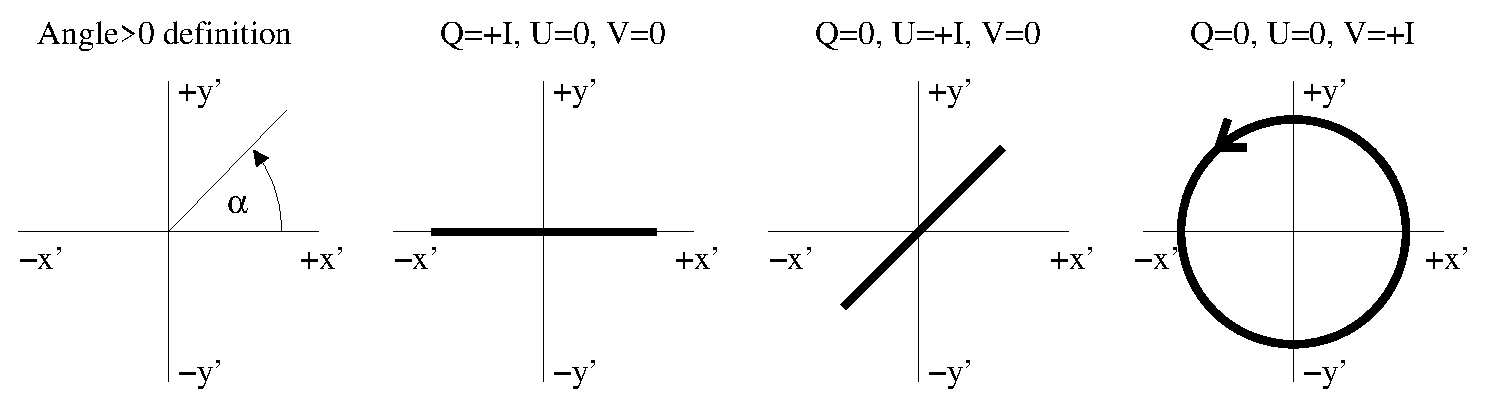
\includegraphics[width=0.9\textwidth]{stokes_and_angles_iaudef.eps}}
\caption{\label{fig-stokes-definition} The definition of the Stokes
  parameters used in RADMC-3D, which is consistent with the IAU 1974
  definitions (see Hamaker \& Bregman (1996) A\&AS 117, pp.161). First panel
  shows that positive angle means counter-clockwise. In the second to fourth
  panels the fat lines show how the tip of the real electric field vector
  goes as a function of time for an observer at a fixed location in space
  watching the radiation. The radiation moves toward the reader. We call the
  second panel ($Q=+I$) ``horizontally polarized'', the third panel ($U=+I$)
  ``diagonally polarized by +45 degrees'' and the fourth panel ($V=+I$)
  ``right-handed circularly polarized''. In the images produced by RADMC-3D
  ({\small\tt image.out}, see Section \ref{sec-image-out} and
  Fig.~\ref{fig-cameraorient}) the $x'$ direction is the horizontal
  direction and the $y'$ direction is the vertical direction.}
\end{figure}
%


We can put these definitions into the standard formulae:
\begin{eqnarray}
Q &=& I\cos(2\beta)\cos(2\chi)\\
U &=& I\cos(2\beta)\sin(2\chi)\\
V &=& I\sin(2\beta)
\end{eqnarray}

The angle $\chi$ is the angle of the E-field in the $(x',y')$ coordinates,
measured counter-clockwise from $x'$ (consistent with our definition
of angles). Example: $\chi$ = 45 deg = $\pi/4$, then $\cos(2\chi)=0$ and
$\sin(2\chi)=1$, meaning that $Q=0$ and $U/I=+1$. Indeed this is consistent 
with the above definition that $U/I=+1$ is $E_x'=E_y'$. 

The angle $2\beta$ is the phase difference between the $y'$-component of the
E-field and the $x'$-component of the E-field such that for $0<\beta<\pi/2$
the E-field rotates in a counter-clockwise sense. In other words: the
$y'$-wave lags $2\beta$ behind the $x'$ wave. Example: if we have
$\beta=\pi/4$, i.e.  $2\beta=\pi/2$, then $\cos(2\beta)=0$ and
$\sin(2\beta)=1$, so we have $Q=U=0$ and $V/I=+1$. This corresponds to the
$y'$ wave being lagged $\pi/2$ behind the $x'$ wave, meaning that we have a
counter-clockwise rotation. If we use the right-hand-rule and point the
thumb into the direction of propagation (toward us) then the fingers indeed
point in counter-rotating direction, meaning that $V/I=+1$ is righthanded
polarized radiation.

In terms of the {\em real} electric fields of a plane monochromatic wave:
\begin{eqnarray}
  E_x'(t) &=& E_h \cos(\omega t-\Delta_h)\\
  E_y'(t) &=& E_v \cos(\omega t-\Delta_v)
\end{eqnarray}
(with $E_h>0$ and $E_v>0$ and $\Delta_{h,v}$ are the phase lags of the
components with respect to some arbitrary phase) we can write the Stokes
components as:
\begin{eqnarray}
  I &=& E_h^2 + E_v^2 \\
  Q &=& E_h^2 - E_v^2\\
  U &=& 2 E_h E_v \cos(\Delta) \\
  V &=& 2 E_h E_v \sin(\Delta)
\end{eqnarray}
with $\Delta = \Delta_v - \Delta_h = 2\beta$.

In terms of the {\em complex} electric fields of a plane monochromatic wave
(the sign before the $i\omega t$ is important):
\begin{eqnarray}
  E_x'(t) &=& E_h e^{i(\Delta_h-\omega t)}\\
  E_y'(t) &=& E_v e^{i(\Delta_v-\omega t)}
\end{eqnarray}
(with $E_h>0$ and $E_v>0$ real numbers 
and $\Delta_{h,v}$ are the phase lags of the
components with respect to some arbitrary phase) we can write the Stokes
components as:
\begin{eqnarray}
  I &=& \langle E_{x'}E_{x'}^{*} + E_{y'}E_{y'}^{*}   \rangle\\
  Q &=& \langle E_{x'}E_{x'}^{*} - E_{y'}E_{y'}^{*}   \rangle\\
  U &=& \langle E_{x'}E_{y'}^{*} + E_{y'}E_{x'}^{*}   \rangle\\
  V &=& i\langle E_{x'}E_{y'}^{*} - E_{y'}E_{x'}^{*}  \rangle
\end{eqnarray}


\subsection{Our conventions compared to other literature}
\label{sec-stokes-convent-differences}
The IAU 1974 definition is different from the definitions used in the
Planck mission, for instance. So be careful. There is something said about
this on the website of the healpix software\footnote{
\url{http://healpix.jpl.nasa.gov/html/intronode12.htm}}.

Our definition is also different from the Mishchenko book and papers (see
below). Compared to the books of Mishchenko and Bohren \& Huffman, our
definitions are:
\begin{eqnarray}
 I_{\mathrm{ours}} &=  I_{\mathrm{mishch}}  &= I_{\mathrm{bohrenhuffman}} \\
 Q_{\mathrm{ours}} &=  Q_{\mathrm{mishch}}  &= Q_{\mathrm{bohrenhuffman}} \\
 U_{\mathrm{ours}} &=  -U_{\mathrm{mishch}} &= -U_{\mathrm{bohrenhuffman}} \\
 V_{\mathrm{ours}} &=  -V_{\mathrm{mishch}} &= -V_{\mathrm{bohrenhuffman}}
\end{eqnarray}
As you see: only the $U$ and $V$ change sign. For a 4$\times$4 M\"uller
matrix $M$ this means that the $M_{II}$, $M_{IQ}$, $M_{QI}$, $M_{QQ}$, as
well as the $M_{UU}$, $M_{UV}$, $M_{VU}$, $M_{VV}$ stay the same, while
$M_{IU}$, $M_{IV}$, $M_{QU}$, $M_{QV}$, as well as $M_{UI}$, $M_{UQ}$,
$M_{VI}$, $M_{VQ}$ components would flip sign.

Compared to Mishchenko, Travis \& Lacis book, what we call $x'$ they call
$\theta$ and what we call $y'$ they call $\phi$. In their Figure 1.3 (which
describes the definition of the Stokes parameters) they have the $\theta$
direction pointing downward, rather than toward the right, i.e.\ rotated by
90 degrees clockwise compared to RADMC-3D. However, since RADMC-3D does not
know what ``right'' or ``down'' are (only what $x'$ and $y'$ are) this
rotation is merely a difference in how we plot things in a figure, and has
no consequences for the results, as long as we define how $x'$ and $y'$ are
oriented compared to our model (see Fig.~\ref{fig-cameraorient} where
$x_{\mathrm{image}}$ is our $x'$ here and likewise for $y'$).

Bohren \& Huffman have the two unit vectors plotted in the following way:
${\bf e}_{\parallel}$ is plotted horizontally to the left and ${\bf
  e}_{\perp}$ is plotted vertically upward. Compared to us, our $x'$ points
toward {\em minus} their ${\bf e}_{\parallel}$, while our $y'$ points toward
their ${\bf e}_{\perp}$, but since they plot their ${\bf e}_{\parallel}$ to
the left, the orientation of our plot and their plots are consistent (i.e.\
if they say ``pointing to the right'', they mean the same direction as
we). But their definition of ``right-handed circular polarization''
(clockwise when seen toward the source of the radiation) is our ``left
handed''.

The book by Wendisch \& Yang ``Theory of Atmospheric Radiative Transfer''
uses the same conventions as Bohren \& Huffman, but their basis vector ${\bf
  e}_{\parallel}$ is plotted vertically and ${\bf e}_{\perp}$ is plotted
horizontally to the right. This only affects what they call ``horizontal'' and
``vertical'' but the math stays the same. 

Our definition is identical to the one on the {\em English} Wikipedia page
on Stokes
parameters\footnote{\url{http://en.wikipedia.org/wiki/Stokes_parameters}}
(on 2 January 2013), with the only exception that what they call
``righthanded'' circularly polarized, we call ``lefthanded''. This is just a
matter of nomenclature of what is right/left-handed, and since RADMC-3D does
not know what ``right/lefthanded'' is, this difference has no further
consequences. {\em Note}, however, that the same Wikipedia page in different
languages use different conventions! For instance, the German version of the
page (on 2 January 2013) has the same Q and U definitions, but has the sign
of V flipped.

Note that in RADMC-3D we have no global definition of the orientation of
$x'$ and $y'$ (see e.g.\ Section \ref{sec-orientation-vector-stokes}). If
we make an image with RADMC-3D, then the horizontal (x-) direction in the
image corresponds to $x'$ and the vertical (y-) direction corresponds to
$y'$, just as one would expect. So if you obtain an image from RADMC-3D
and all the pixels in the image have $Q=I$ and $U=V=0$, then the electric
field points horizontally in the image.

\subsection{Defining orientation for non-observed radiation}
\label{sec-orientation-vector-stokes}
%
To complete our description of the Stokes parameters we still need to define
in which direction we let $x'$ and $y'$ point if we do {\em not} have an
obvious observer, i.e.\ for radiation moving through our object of interest
which may never reach us. In the Monte Carlo modules of RADMC-3D, when
polarization is switched on, any photon package does not only have a
wavelength $\lambda$ and a direction of propagation ${\bf n}$ associated
with it, but also a second unit vector ${\bf S}$, which is always assured
to obey:
\begin{equation}
|{\bf S}| = 1 \qquad \hbox{and} \qquad {\bf S}\cdot{\bf n}=0
\end{equation}
This leaves, for a given ${\bf n}$, one degree of freedom (any direction as
long as it is perpendicular to ${\bf n}$). It is irrelevant which direction
is chosen for this, but whatever choice is made, it sets the definitions
of the $x'$ and $y'$ directions. The definitions are:
\begin{equation}
\begin{split}
x' & \quad\hbox{points in the direction}\quad {\bf S}\times {\bf n}\\
y' & \quad\hbox{points in the direction}\quad {\bf S}\\
z' & \quad\hbox{points in the direction}\quad {\bf n}
\end{split}
\end{equation}
So for $Q=-I$, $U=V=0$ the electric field points in the direction of
${\bf S}$, while for $Q=+I$, $U=V=0$ it is perpendicular to both
${\bf n}$ and ${\bf S}$. 

However, if you are forced to change the direction of ${\bf S}$ for whatever
reason, the Stokes components will also change. This coordinate transformation
works as follows.
We can transform from a '-basis to a ''-basis by rotating the ${\bf S}$-vector
counter-clockwise (as seen by the observer watching the radiation) by an
angle $\alpha$. Any vector $(x',y')$ in the '-basis will become a vector
$(x'',y'')$ in a ''-basis, given by the transformation:
\begin{equation}
\left(\begin{matrix}
x''\\y''
\end{matrix}\right)
=
\left(\begin{matrix}
\cos(\alpha) & \sin(\alpha)\\
-\sin(\alpha) & \cos(\alpha)
\end{matrix}\right)
\left(\begin{matrix}
x'\\y'
\end{matrix}\right)
\end{equation}
NOTE: We choose $(x',y')$ to be the usual counter-clockwise basis for the
observer seeing the radiation. Rotating the basis in counter-clockwise
direction means rotating the vector in that basis in clockwise direction,
hence the sign convention in the matrix. 

If we have $(I,Q,U,V)$ in the '-basis (which we might have written as
$(I',Q',U',V')$ but by convention we drop the '), the $(I'',Q'',U'',V'')$ in
the ''-basis becomes
\begin{equation}
\left(\begin{matrix}
I''\\Q''\\U''\\V''
\end{matrix}\right)
=
\left(\begin{matrix}
1 & 0 & 0 & 0 \\
0 & \cos(2\alpha) & \sin(2\alpha) & 0 \\
0 & -\sin(2\alpha) & \cos(2\alpha) & 0 \\
0 & 0 & 0 & 1
\end{matrix}\right)
\left(\begin{matrix}
I\\Q\\U\\V
\end{matrix}\right)
\end{equation}



\subsection{Polarized scattering off dust particles: general formalism}
Suppose we have {\em one} dust particle of mass $m_{\mathrm{grain}}$ and we
place it at location ${\bf x}$. Suppose this particle is exposed to a plane
wave of electromagnetic radiation pointing in direction ${\bf
  n}_{\mathrm{in}}$ with a flux ${\bf F}_{\mathrm{in}}=F_{\mathrm{in}}\,{\bf
  n}_{\mathrm{in}}$. This radiation can be polarized, so that
$F_{\mathrm{in}}$ actually is a Stokes vector:
\begin{equation}
F_{\mathrm{in}} = \left(\begin{matrix}
F_{I,\mathrm{in}}\\
F_{Q,\mathrm{in}}\\
F_{U,\mathrm{in}}\\
F_{V,\mathrm{in}}
\end{matrix}\right)
\end{equation}
This particle will scatter some of this radiation into all directions. 
What will the flux of scattered radiation be, as observed at location
${\bf y}\neq{\bf x}$? Let us define the vector
\begin{equation}
{\bf r} = {\bf y} - {\bf x}
\end{equation}
its length
\begin{equation}
r = |{\bf r}|
\end{equation}
and the unit vector
\begin{equation}
{\bf e}_r = \frac{{\bf r}}{r}
\end{equation}
We will assume that $r\gg a$ where $a$ is the particle size. 
We define the {\em scattering matrix elements} $Z_{ij}$ (with $i,j$ =
$1,2,3,4$) such that the measured outgoing flux from the particle
at ${\bf y}$ is
\begin{equation}
{\bf F}_{\mathrm{out}} = F_{\mathrm{out}}{\bf e}_r
\end{equation}
with
\begin{equation}
F_{\mathrm{out}} = \left(\begin{matrix}
F_{I,\mathrm{out}}\\
F_{Q,\mathrm{out}}\\
F_{U,\mathrm{out}}\\
F_{V,\mathrm{out}}
\end{matrix}\right)
=\frac{m_{\mathrm{grain}}}{r^2}
\left(\begin{matrix}
Z_{11} & Z_{12} & Z_{13} & Z_{14} \\
Z_{21} & Z_{22} & Z_{23} & Z_{24} \\
Z_{31} & Z_{32} & Z_{33} & Z_{34} \\
Z_{41} & Z_{42} & Z_{43} & Z_{44}
\end{matrix}\right)
\left(\begin{matrix}
F_{I,\mathrm{in}}\\
F_{Q,\mathrm{in}}\\
F_{U,\mathrm{in}}\\
F_{V,\mathrm{in}}
\end{matrix}\right)
\end{equation}
The values $Z_{ij}$ depend on the direction into which the radiation is
scattered (i.e.\ ${\bf e}_r$) and on the direction of the incoming flux
(i.e.\ ${\bf n}$), but not on $r$: the radial dependence of the outgoing
flux is taken care of through the $1/r^2$ factor in the above formula.

Some notes about our conventions are useful at this place. In many books the
``scattering matrix'' is written as $F_{ij}$ instead of $Z_{ij}$, and is
defined as the $Z_{ij}$ for the case when radiation comes from one
particular direction: ${\bf n}=(0,0,1)$. In this manual and in the RADMC-3D
code, however, we will always write $Z_{ij}$, because the symbol $F$ can be
confused with flux. The normalization of these matrix elements is also
different in different books. In our case it has the dimension
cm$^2$/gram/steradian. The conversion from the conventions of other books is
(where $k=2\pi/\lambda$ is the wave number in units of 1/cm):
\begin{equation}
Z_{ij,\mathrm{RADMC-3D}} = \frac{Z_{ij,\mathrm{Mishchenko}}}{m_{\mathrm{grain}}}
= \frac{S_{ij,\mathrm{BohrenH}}}{k^2m_{\mathrm{grain}}}
\end{equation}
except that for the $Z_{13}$, $Z_{14}$, $Z_{23}$, $Z_{24}$, $Z_{31}$,
$Z_{41}$, $Z_{32}$, $Z_{42}$ elements (if non-zero) there must be a minus
sign before the $Z_{ij,\mathrm{RADMC-3D}}$ because of the opposite $U$ and
$V$ sign conventions (see Section \ref{sec-stokes-convent-differences}).

Note that the $S_{ij,\mathrm{BohrenH}}$ are the matrix elements obtained
from the famous {\small\tt BHMIE.F} code from the Bohren \& Huffman book
(see Chapter \ref{chap-acquiring-opacities}). 

\subsection{Polarized scattering off dust particles: randomly oriented particles}
In the special case in which we either have spherical particles or we
average over a large number of randomly oriented particles, the $Z_{ij}$
elements are no longer dependent on {\em both} ${\bf e}_r$ and {\bf n} but
only on the angle between them:
\begin{equation}
\cos\theta = {\bf n}\cdot{\bf e}_r
\end{equation}
So we go from $Z_{ij}({\bf n},{\bf e}_r)$, i.e.\ a four-angle dependence, to
$Z_{ij}(\theta)$, i.e.\ a one-angle dependence. 

Now let us also assume that there is no netto helicity of the particles
(they are either axisymmetric or there exist equal amounts of particles
as their mirror symmetric counterparts). In that case (see e.g.\ 
Mishchenko book) of the 16 matrix elements only 6 are non-zero and independent:
\begin{equation}
F_{\mathrm{out}} = \left(\begin{matrix}
F_{I,\mathrm{out}}\\
F_{Q,\mathrm{out}}\\
F_{U,\mathrm{out}}\\
F_{V,\mathrm{out}}
\end{matrix}\right)
=\frac{m_{\mathrm{grain}}}{r^2}
\left(\begin{matrix}
Z_{11} & Z_{12} & 0 & 0 \\
Z_{12} & Z_{22} & 0 & 0 \\
0 & 0 & Z_{33} & Z_{34} \\
0 & 0 & -Z_{34} & Z_{44}
\end{matrix}\right)
\left(\begin{matrix}
F_{I,\mathrm{in}}\\
F_{Q,\mathrm{in}}\\
F_{U,\mathrm{in}}\\
F_{V,\mathrm{in}}
\end{matrix}\right)
\label{eq-scatmat-for-randorient-nohelic}
\end{equation}
This is the case for scattering in RADMC-3D. Note that in Mie scattering
the number of independent matrix elements reduces to just 4 because 
then $Z_{22}=Z_{11}$ and $Z_{44}=Z_{33}$. But RADMC-3D also allows for
cases where $Z_{22}\neq Z_{11}$ and $Z_{44}\neq Z_{33}$, i.e.\ for
opacities resulting from more detailed calculations such as DDA or 
T-matrix calculations.

Now, as described above, the Stokes vectors only have meaning if the
directions of $x'$ and $y'$ are well-defined. For
Eq.~(\ref{eq-scatmat-for-randorient-nohelic}) to be valid (and for the
correct meaning of the $Z_{ij}$ elements) the following definition is used:
Before the scattering, the ${\bf S}$-vector of the photon package is rotated
(and the Stokes vectors accordingly transformed) such that the new ${\bf
  S}$-vector is perpendicular to both ${\bf n}$ and ${\bf e}_r$. In other
words, the scattering angle $\theta$ is a rotation of the photon propagation
around the (new) ${\bf S}$-vector. The sign convention is such that
\begin{equation}
({\bf n}\times {\bf e}_r)\cdot{\bf S}=\sin(\theta)
\end{equation}
In other words, if we look into the incoming light (with $z'$ pointing
toward us), then for $\sin(\theta)>0$ the photon is scattered into the
$x'>0$, $y'=0$ direction (i.e.\ for us it is scattered to the right).
The ${\bf S}$ vector for the outgoing photon remains unchanged, since
the new ${\bf n}$ is also perpendicular to it.

So what does this all mean for the opacity? The scattering opacity tells us
how much of the incident radiation is removed and converted into outgoing
scattered radiation. The absorption opacity tells us how much of the
incident radiation is removed and converted into heat. For randomly oriented
particles without netto helicity both opacities are independent of the
polarization state of the radiation. Moreover, the thermal emission
is unpolarized in this case. This means that in the radiative
transfer equation the extinction remains simple:
\begin{equation}\label{eq-radtrans-randomorient}
\frac{d}{ds}\left(
\begin{matrix}
I_I\\I_Q\\I_U\\I_V
\end{matrix}
\right)
=
\left(
\begin{matrix}
j_{\mathrm{emis},I}\\0\\0\\0
\end{matrix}
\right)
+
\left(
\begin{matrix}
j_{\mathrm{scat},I}\\j_{\mathrm{scat},Q}\\j_{\mathrm{scat},U}\\j_{\mathrm{scat},V}
\end{matrix}
\right)
-\rho(\kappa_{\mathrm{abs}}+\kappa_{\mathrm{scat}})
\left(
\begin{matrix}
I_I\\I_Q\\I_U\\I_V
\end{matrix}
\right)
\end{equation}
where $I_I$, $I_Q$, $I_U$, $I_V$ are the intensities (erg/s/cm$^2$/Hz/ster)
for the four Stokes parameters, and likewise for $j_{\mathrm{emis}}$ and
$j_{\mathrm{scat}}$, and finally, $s$ the path length along the ray under
consideration. Note that if we would allow for fixed-orientation dust
particles (which we don't), Eq.~(\ref{eq-radtrans-randomorient}) would
become considerably more complex, with extinction being matrix-valued and
thermal emission being polarized.

Since $\kappa_{\mathrm{scat}}$ converts incoming radiation into outgoing
scattered radiation, it should be possible to calculate 
$\kappa_{\mathrm{scat}}$ from angular integrals of the scattering
matrix elements. For randomly oriented non-helical particles we indeed
have:
\begin{equation}\label{eq-scatmat-selfconsist-kappa}
\kappa_{\mathrm{scat}} = \oint Z_{11} d\Omega = 
2\pi \int_{-1}^{+1}Z_{11}(\mu)d\mu
\end{equation}
where $\mu=\cos\theta$. In a similar exercise we can calculate the
anisotropy factor $g$ from the scattering matrix elements:
\begin{equation}\label{eq-scatmat-selfconsist-g}
g = \frac{2\pi}{\kappa_{\mathrm{scat}}}\int_{-1}^{+1}Z_{11}(\mu)\mu d\mu
\end{equation}

This essentially completes the description of scattering as it is
implemented in RADMC-3D.

We can precalculate the $Z_{ij}(\theta)$ for every wavelength and for a
discrete set of values of $\theta$, and store these in a table. This is
indeed the philosophy of RADMC-3D: You have to precompute them using, for
instance, the Mie code of Bohren and Huffman (see Chapter
\ref{chap-acquiring-opacities} for RADMC-3D compliant wrappers around that
code), and then provide them to RADMC-3D through a file called {\small\tt
  dustkapscatmat\_xxx.inp} (where {\small\tt xxx} is the name of the dust
species) which is described in Section \ref{sec-dustkapscatmat-files}.  This
file provides not only the matrix elements, but also the
$\kappa_{\mathrm{abs}}$, $\kappa_{\mathrm{scat}}$ and $g$ (the anisotropy
factor). RADMC-3D will then internally check that
Eqs.(\ref{eq-scatmat-selfconsist-kappa}, \ref{eq-scatmat-selfconsist-g}) are
indeed fulfilled. If not, an error message will result.

One more note: As mentioned in Section \ref{sec-definitions-stokes}, the
sign conventions of the Stokes vector components we use (the IAU 1974
definition) are different from the Bohren \& Huffman and Mishchenko
books. For randomly oriented particles, however, the sign conventions of the
$Z$-matrix elements are not affected, because those matrix elements that
would be affected are those that are in the upper-right and lower-left
quadrants of the matrix, and these elements are anyway zero. So we can use,
for randomly oriented particles, the matrix elements from those books and
their computer codes without having to adjust the signs.

\subsection{Scattering and axially symmetric models}
In spherical coordinates it is possible in RADMC-3D to set up axially
symmetric models. The trick is simply to set the number of $\phi$ coordinate
points {\small\tt nphi} to 1 and to switch off the $\phi$-dimension in the
grid (see Section \ref{sec-grid-input}). For isotropic scattering this mode
has always been implemented. But for anisotropic scattering things become
more complex. For such a model the scattering remains a fully 3-D problem:
the scattering source function has to be stored not only as a function of
$r$ and $\theta$, but also as a function of $\phi$ (for a given observer
vantage point). The reason is that anisotropic scattering {\em does} care
about viewing angle (in contrast to isotropic scattering). So even though
for an axisymmetric model the density and temperature functions only depend
on $r$ and $\theta$ (and are therefore mathematically 2-D), the scattering
source function depends on $r$, $\theta$ and $\phi$.

For this reason anisotropic scattering was, until version 0.40, not allowed
for 2-D axisymmetric models. As of version 0.41 it is now possible to use
the full polarized scattering mode ({\small\tt scattering\_mode=5}) also for
2-D axisymmetric models. The intermediate scattering modes ({\small\tt
  scattering\_mode=2, 3, 4}) remain incompatible with 2-D axisymmetry.
Isotropic scattering remains, as before, fully compatible with 2-D
axisymmetry.

One note of explanation: the way the full scattering is now implemented into
the case of 2-D axisymmetry is the following: internally we compute not just
the scattering source function for one angle, but for a whole set of $\phi$
angles (even though the grid has no $\phi$-points). Each time a photon in
the scattering Monte Carlo simulation enters a cell (which in 2-D
axisymmetry is an annulus), a loop over 360 $\phi$ angles is performed, and
the scattering source function is computed for all of these angles.  {\em
  This makes the code rather slow for each photon package!} But one needs
fewer photon packages to get sufficiently high signal-to-noise ratio. You
can experiment with fewer $\phi$ angles by adding, in {\small\tt radmc3d.inp},
the following line (as an example):
{\small\begin{verbatim}
dust_2daniso_nphi = 60
\end{verbatim}}
in which case instead of 360 the model will only use 60 $\phi$ points. That
will speed up the code significantly, but of course will treat the
$\phi$-dependence of the scattering source function with lower precision.

For now the 2-D axisymmetric version of full scattering is only possible 
with first-order integration. 



\section{More about photon packages in the Monte Carlo simulations}
\label{sec-photon-packages-mc}
%
In the ``standard'' Monte Carlo approach, the input energy (e.g.\ starlight
or, for the scattering Monte Carlo, the thermal emission of dust) is divided
into $N$ equal energy packages of photons, which then travel through the
model and eventually either escape or get destroyed. This equal division
scheme is, however, problematic for some model setups. For instance, if you
have stars with vastly different luminosity in the model, then the brightest
of these stars will dominate, by far, the number of output photon packages.
This means that the material around low-brightness stars (which, by their
proximity to these low-brightness stars, are still dominated by heating by
these low-brightness stars) will experience very bad photon statistics.

To avoid this problem, RADMC-3D has, by default, its ``weighted photon
package mode'' switched on. This will make sure that each source of 
energy (i.e.\ each star, but also each other type of source) emits the
same amount of photons. Only: bright stars will emit more energetic
photon packages than dim stars. 

The ``weighted photon package mode'' will also solve another problem.
Suppose a star lies far outside of the grid. It will emit most of its
photons in directions that completely miss the grid. This means that
RADMC-3D would waste a lot of time drawing random numbers for photons that
will anyway not affect the model. Also here the ``weighted photon package
mode'' solves the problem: It will focus the photon packages toward the
model grid, and lower their energy to compensate for their favorable
focusing toward the grid.

{\em NOTE:} Since RADMC-3D is still in beta-phase, and both aspects of the
``weighted photon package mode'' meddle with the standard equal-weighting
procedure, it might be useful to sometimes check the results against a run
without this mode but with a huge number of photon packages to compensate -
just to check if there are no bugs or other subtleties. You can switch the
mode off by setting {\small\tt mc\_weighted\_photons}=0 in the {\small\tt
  radmc3d.inp} file.


\section{Polarized emission and absorption by aligned grains}
\label{sec-polarized-thermal-emission}
%
{\bf NOTE: This mode is still in the testing phase (February 2017)!}

Grain alignment and its effects on radiative transfer is a complex topic. A
review is e.g.~Andersson, B.G., Lazarian, A., \& Vaillancourt, J.E.\ (2015)
``Interstellar Dust Grain Alignment'', Annual Review of Astronomy and
Astrophysics, 53(1), 501–539. In RADMC-3D grain alignment is included only
in a limited form. First and foremost: RADMC-3D does not know about the
physics {\em causing} the grain alignment. You, the user, will have to tell
how the grain are aligned by giving the code a directional vector field and
for each wavelength the degree to which the grain is aligned to that
directional vector (more on this later). This is according to the RADMC-3D
philosophy of doing {\em only} the radiative transfer and leaving the
physics of the material to the user.

\subsection{Basics}
\label{sec-basic-equations}
%
Suppose we have flattened (oblate) ellipsoidal grains with one axis of
symmetry and no helicity\footnote{While helicity may be needed to
  radiatively spin up grains, we assume that on average the helicity of the
  grains is zero.}. Let us assume that they are aligned with that symmetry
axis along the $y$-axis. We view radiation from the point where the $z$-axis
points toward us. Horizontally polarized light (which has $E$-field in
horizontal direction, i.e.\ in $x$-direction) has $Q/I=+1$, vertically
polarized light (with the $\vec E$ vector aligned with the symmetry axis of
the grain) has $Q/I=-1$. We can then assume that the dust has different
extinction coefficients for the horizontal and vertical axis. Let us call
these:
\begin{eqnarray}
\alpha_{\mathrm{abs},\nu,\mathrm{h}} &\equiv& \rho_d\kappa_{\mathrm{abs},\nu,\mathrm{h}}\\
\alpha_{\mathrm{abs},\nu,\mathrm{v}} &\equiv& \rho_d\kappa_{\mathrm{abs},\nu,\mathrm{v}}
\end{eqnarray}
%The 'E' stands for electric field, the 'M' for magnetic field. These are the
%nomenclature of Wolf et al.~A\&A 385, 365 (2002). {\em Question: Check out
%if his E and M are not swapped...}

We can define $I$, $Q$, $U$ and $V$ in terms of the electric field
components $E_x$ and $E_y$. The electric field components for a perfectly
coherent wave can be written as
\begin{eqnarray}
E_x&=&E_{x,0}\cos(\omega t-\Delta_x)\\
E_y&=&E_{y,0}\cos(\omega t-\Delta_y)
\end{eqnarray}
where $\Delta_x$ and $\Delta_y$ are phase lags. The phase lag between
the $y$ and $x$-fields is $\Delta=\Delta_y-\Delta_x$, meaning that for
positive $\Delta$ the $y$-field lags behind the $x$-field. We then 
define the Stokes components as:
\begin{eqnarray}
I &=& E_{x,0}^2+E_{y,0}^2\label{eq-def-stokes-i}\\
Q &=& E_{x,0}^2-E_{y,0}^2\label{eq-def-stokes-q}\\
U &=& 2E_{x,0}E_{y,0}\cos\Delta\label{eq-def-stokes-u}\\
V &=& 2E_{x,0}E_{y,0}\sin\Delta\label{eq-def-stokes-v}
\end{eqnarray}
Note that for $V=I$ ($\Delta=\pi/2$, i.e.\ the $E_y$ lags $\pi/2$ behind
$E_x$) we have {\em right-handed} circularly polarized light, meaning that
the tip of the $\vec E$ field at a fixed point in space, when looking into
the light (the propagation of light is toward the reader) rotates
counter-clockwise (when the $x$-coordinate points right, and the
$y$-coordinate points up). The 3-D helix of his field will be {\em
  left-handed} (when the z-coordinate points into the propagation direction
of the light, i.e. toward the reader, i.e.\ a right-handed coordinate
system). For $Q=I$ we have linearly polarized light in which the $\vec
E$-field lies in the $x$-direction. For $U=I$ we have linearly polarized
light in which $\vec E$ lies along the $x=y$ line (when looking into the
light). These definitions are consistent with the IAU 1974 definitions
(Hamaker \& Bregman 1996, A\&AS 117, pp.161).

The $E_x$ and $E_y$ get absorbed in the following way:
\begin{eqnarray}
E_{x,0}' &=& E_{x,0} e^{-\tfrac{1}{2}\alpha_{\mathrm{abs},\nu,\mathrm{h}}s}\\
E_{y,0}' &=& E_{y,0} e^{-\tfrac{1}{2}\alpha_{\mathrm{abs},\nu,\mathrm{v}}s}
\end{eqnarray}
where $s$ is a length along the ray.

For this kind of problem it is convenient to introduce the so-called {\em
  modified Stokes parameters} $I_{\mathrm{h}}$ and $I_{\mathrm{v}}$:
\begin{eqnarray}
I_{\mathrm{h}} &=& \frac{1}{2}(I+Q)\label{eq-modif-stokes-h}\\
I_{\mathrm{v}} &=& \frac{1}{2}(I-Q)\label{eq-modif-stokes-v}
\end{eqnarray}
so that we have 
\begin{eqnarray}
I &=& I_{\mathrm{h}}+I_{\mathrm{v}}\\
Q &=& I_{\mathrm{h}}-I_{\mathrm{v}}
\end{eqnarray}
so that one can say, for perfectly coherent light,
\begin{eqnarray}
I_{\mathrm{h}} &=& E_{x,0}^2\\
I_{\mathrm{v}} &=& E_{y,0}^2
\end{eqnarray}
With this we get the following extinction law:
\begin{eqnarray}
I_{\mathrm{h}}' &=& I_{\mathrm{h}} e^{-\alpha_{\mathrm{abs},\nu,\mathrm{h}}s}\\
I_{\mathrm{v}}' &=& I_{\mathrm{v}} e^{-\alpha_{\mathrm{abs},\nu,\mathrm{v}}s}
\end{eqnarray}

How do $U$ and $V$ extinct? If we use Eqs.~(\ref{eq-def-stokes-u},
\ref{eq-def-stokes-v}), and assume that the phase lag $\Delta$ will not
change during the extinction, then 
\begin{equation}
\begin{split}
U' &= U e^{-\tfrac{1}{2}\alpha_{\mathrm{abs},\nu,\mathrm{h}}s} e^{-\tfrac{1}{2}\alpha_{\mathrm{abs},\nu,\mathrm{v}}s}\\
&=U e^{-\tfrac{1}{2}(\alpha_{\mathrm{abs},\nu,\mathrm{h}}+\alpha_{\mathrm{abs},\nu,\mathrm{v}})s}
\end{split}
\end{equation}
This means that 
\begin{equation}
\alpha_{\mathrm{abs},\nu,\mathrm{uv}} =
\frac{1}{2}\left(\alpha_{\mathrm{abs},\nu,\mathrm{h}}+\alpha_{\mathrm{abs},\nu,\mathrm{v}}\right)
\end{equation}
and
\begin{eqnarray}
I_{\mathrm{u}}' &=& I_{\mathrm{u}} e^{-\alpha_{\mathrm{abs},\nu,\mathrm{uv}}s}\\
I_{\mathrm{v}}' &=& I_{\mathrm{v}} e^{-\alpha_{\mathrm{abs},\nu,\mathrm{uv}}s}
\end{eqnarray}
In matrix notation
\begin{equation}
\frac{d}{ds}
\left(\begin{matrix}
I_{\mathrm{h}} \\
I_{\mathrm{v}} \\
U \\
V \\
\end{matrix}\right)
= - 
\left(\begin{matrix}
\alpha_{\mathrm{h}} & 0 & 0 & 0 \\
0 & \alpha_{\mathrm{v}} & 0 & 0  \\
0 & 0 & \alpha_{\mathrm{uv}} & 0 \\
0 & 0 & 0 & \alpha_{\mathrm{uv}} \\
\end{matrix}\right)
\left(\begin{matrix}
I_{\mathrm{h}} \\
I_{\mathrm{v}} \\
U \\
V \\
\end{matrix}\right)
\end{equation}
If we translate this to the usual Stokes components we get
\begin{equation}
\frac{d}{ds}
\left(\begin{matrix}
I \\
Q \\
U \\
V \\
\end{matrix}\right)
= - 
\left(\begin{matrix}
\alpha_1 & \alpha_2 & 0 & 0 \\
\alpha_2 & \alpha_1 & 0 & 0  \\
0 & 0 & \alpha_1 & 0 \\
0 & 0 & 0 & \alpha_1 \\
\end{matrix}\right)
\left(\begin{matrix}
I \\
Q \\
U \\
V \\
\end{matrix}\right)
\end{equation}
with
\begin{eqnarray}
\alpha_1 &=& \frac{1}{2}\left(\alpha_{\mathrm{abs},\nu,\mathrm{h}}+\alpha_{\mathrm{abs},\nu,\mathrm{v}}\right) 
= \alpha_{\mathrm{abs},\nu,\mathrm{uv}}\\
\alpha_2 &=& \frac{1}{2}\left(\alpha_{\mathrm{abs},\nu,\mathrm{h}}-\alpha_{\mathrm{abs},\nu,\mathrm{v}}\right) 
\end{eqnarray}

The emission will be also independently in horizontal and vertical
direction. But nothing will be emitted in U or V direction. So it is most
convenient to express the emission/absorption process in terms of the
modified Stokes parameters:
\begin{eqnarray}
\frac{dI_{\nu,\mathrm{h}}}{ds} &=& \alpha_{\mathrm{abs},\nu,\mathrm{h}} (\frac{1}{2}B_\nu(T)-I_{\nu,\mathrm{h}}) \\
\frac{dI_{\nu,\mathrm{v}}}{ds} &=& \alpha_{\mathrm{abs},\nu,\mathrm{v}} (\frac{1}{2}B_\nu(T)-I_{\nu,\mathrm{v}}) \\
\frac{dU_{\nu}}{ds} &=& -\alpha_{\mathrm{abs},\nu,\mathrm{uv}} U_{\nu} \\
\frac{dV_{\nu}}{ds} &=& -\alpha_{\mathrm{abs},\nu,\mathrm{uv}} V_{\nu}
\end{eqnarray}
In terms of matrix notation this becomes
\begin{equation}\label{eq-formal-rt-emisabs-in-rotated-system}
\frac{d}{ds}
\left(\begin{matrix}
I_{\mathrm{h}} \\
I_{\mathrm{v}} \\
U \\
V \\
\end{matrix}\right)
= \left(\begin{matrix}
\tfrac{1}{2}\alpha_{\mathrm{h}} B_\nu(T) \\
\tfrac{1}{2}\alpha_{\mathrm{v}} B_\nu(T) \\
0 \\
0 \\
\end{matrix}\right)
- 
\left(\begin{matrix}
\alpha_{\mathrm{h}} & 0 & 0 & 0 \\
0 & \alpha_{\mathrm{v}} & 0 & 0  \\
0 & 0 & \alpha_{\mathrm{uv}} & 0 \\
0 & 0 & 0 & \alpha_{\mathrm{uv}} \\
\end{matrix}\right)
\left(\begin{matrix}
I_{\mathrm{h}} \\
I_{\mathrm{v}} \\
U \\
V \\
\end{matrix}\right)
\end{equation}
In terms of the normal Stokes parameters this becomes
\begin{equation}
\frac{d}{ds}
\left(\begin{matrix}
I \\
Q \\
U \\
V \\
\end{matrix}\right)
= \left(\begin{matrix}
\alpha_1 B_\nu(T) \\
\alpha_2 B_\nu(T) \\
0 \\
0 \\
\end{matrix}\right)
- 
\left(\begin{matrix}
\alpha_1 & \alpha_2 & 0 & 0 \\
\alpha_2 & \alpha_1 & 0 & 0  \\
0 & 0 & \alpha_1 & 0 \\
0 & 0 & 0 & \alpha_1 \\
\end{matrix}\right)
\left(\begin{matrix}
I \\
Q \\
U \\
V \\
\end{matrix}\right)
\end{equation}
or written slightly differently:
\begin{equation}
\frac{d}{ds}
\left(\begin{matrix}
I \\
Q \\
U \\
V \\
\end{matrix}\right)
=  
\left(\begin{matrix}
\alpha_1 & \alpha_2 & 0 & 0 \\
\alpha_2 & \alpha_1 & 0 & 0  \\
0 & 0 & \alpha_1 & 0 \\
0 & 0 & 0 & \alpha_1 \\
\end{matrix}\right)
\left[
\left(\begin{matrix}
B_\nu(T) \\
0 \\
0 \\
0 \\
\end{matrix}\right)
-\left(\begin{matrix}
I \\
Q \\
U \\
V \\
\end{matrix}\right)\right]
\end{equation}


So to sum things up: We need only the absorption opacity for light with
$\vec E$ perpencidular to the symmetry axis ($\kappa_{\mathrm{abs},\nu,h}$)
and the absorption opacity for light with $\vec E$ parallel to the symmetry
axis ($\kappa_{\mathrm{abs},\nu,v}$).

% However, there is still a little catch: The grain can have an angle $\xi$
% with respect to the $y$-axis in the $y-z$ plane. We define the angle $\xi$
% such that the symmetry axis of the grain $\vec n$ is:
% \begin{equation}
% \vec n=\left(\begin{matrix}
% 0 \\
% \cos\xi \\
% \sin\xi
% \end{matrix}\right)
% \end{equation}
% Note that we can always rotate away any angle in the $x-y$-plane, so we only
% need to worry about the angle in the $y-z$-plane. So for every frequency
% $\nu$, for every angle $\xi$ we must specify $\kappa_{\mathrm{h}}$
% (perpendicular to $\vec n$) and $\kappa_{\mathrm{v}}$ (parallel to $\vec
% n$).


\subsection{Implementation in RADMC-3D}
\subsubsection{Polarized emission in the images and spectra}
When creating images (and spectra) the {\small\tt camera} module of RADMC-3D
performs a ray-tracing calculation (``volume renderung'') through the grid.
Normally (for randomly oriented grains) the extinction along the line of
sight is always unpolarized, i.e.\ each Stokes component is extincted
equally much. The thermal emission along the line of sight is also
unpolarized. 

Now, however, we wish to include the effect of grain alignment in the
ray-tracing. We assume that at position $\vec x$ in the grid our oblate
grain is aligned such that the minor axis points in the direction of the
orientation vector $\vec n_{\mathrm{align}}(\vec x)$. If the grain is
prolate, we assume that it spins along one of its minor axes such that this
spin axis is pointing along $\vec n_{\mathrm{align}}(\vec x)$, so that, in
effect, it acts as if it were an oblate grain again. In practice the
alignment vector $\vec n_{\mathrm{align}}(\vec x)$ does not lie always in
the plane of the sky of the observer. Instead it will have an angle $\theta$
with the line-of-sight direction vector $\vec n_{\mathrm{los}}$ (note that
this $\theta$ angle is different from the scattering angle $\theta$), 
defined as
\begin{equation}
\cos\theta \equiv = \left|\vec n_{\mathrm{align}}\cdot 
\vec n_{\mathrm{los}}\right|
\end{equation}
Here we assume that the grains have top/bottom symmetry so that we only
have to concern ourselves with the positive values of $\cos\theta$, hence
the $||$. If $\cos\theta=1$ then we see the oblate grain from the top or
the bottom, so that we do not expect any polarized emission. The strongest
polarized emission is expected when $\cos\theta=0$, which means that the 
oblate grain is seen edge-on. 

We can now define the ``projected alignment vector'' $\vec
n_{\mathrm{align,proj}}$, which is the alignment vector projected into
the image plane:
\begin{equation}
\vec n_{\mathrm{align,proj}} = \vec n_{\mathrm{align}} - (\vec n_{\mathrm{align}}\cdot 
\vec n_{\mathrm{los}})\;\vec n_{\mathrm{los}}
\end{equation}
To use the equations from Section \ref{sec-basic-equations} we must first
rotate our image plane coordinates $(x,y)$ to new coordinates $(x',y')$ such
that the $y'$ (vertical) direction points along the $\vec
n_{\mathrm{align,proj}}$ vector while the $x'$ (horizontal) direction points
perpendicular to it. Let us write the Stokes vector of the radiation along
the line of sight
$(I_{\mathrm{in}},Q_{\mathrm{in}},U_{\mathrm{in}},V_{\mathrm{in}})$, where
we implicitly know that these are also a function of frequency $\nu$. This
Stokes vector is defined with respect to the vector $\vec S$ which is
perpendicular to the line-of-sight direction vector $\vec n_{\mathrm{los}}$
and defines the direction in which the $y$-coordinate of the image plane
points. We must now express this incoming radiation (at the start of the
segment) in the new $(x',y')$ image plane coordinates, i.e.~with respect to
the new vector $\vec S'$ that points along $\vec n_{\mathrm{align,proj}}$
(i.e.~$\vec S'$ is the normalized version of $\vec
n_{\mathrm{align,proj}}$). This rotation is performed using
\begin{equation}\label{eq-rot-stokes-align}
\left(\begin{matrix}
I'\\Q'\\U'\\V'
\end{matrix}\right)
=
\left(\begin{matrix}
1 & 0 & 0 & 0 \\
0 & \cos(2\alpha) & \sin(2\alpha) & 0 \\
0 & -\sin(2\alpha) & \cos(2\alpha) & 0 \\
0 & 0 & 0 & 1
\end{matrix}\right)
\left(\begin{matrix}
I_{\mathrm{in}}\\Q_{\mathrm{in}}\\U_{\mathrm{in}}\\V_{\mathrm{in}}
\end{matrix}\right)
\end{equation}
where $\alpha$ is the angle between $\vec S'$ and $\vec S$ such that if (as
seen by the observer) $\vec S'$ lies counter-clockwise from $\vec S$,
$\alpha$ is positive (the usual definition). With this new Stokes vector
$(I',Q',U',V')$ we will now use the equations of Section
\ref{sec-basic-equations}. 

To be able to perform this rotation in a uniquely defined way, it is
necessary that along each segment along the line of sight this new $(x',y')$
orientation stays fixed (but can vary from segment to segment). As the
line-of-sight ray enters a cell and leaves it again, this line element
(segment) will have its image-plane coordinates rotated according to the
alignment vector of that cell. As a result, the integration must be done
first order (assuming all source terms to be constant along the segment).
In principle second order integration would also be possible, but then the
trick with the rotation of the image coordinate plane such that $y'$ points
along the orientation vector does no longer work, and the integration of the
formal transfer equation would become much more complex, involving the full
M\"uller matrix formulation. We will not do this, so we will stick to first
order integration of Eq.~\ref{eq-formal-rt-emisabs-in-rotated-system}.

For convenience we will leave out the primes (') from here on, so while we
write $(I,Q,U,V)$ we mean in fact $(I',Q',U',V')$. We now compute
$I_{\mathrm{h}}$ and $I_{\mathrm{v}}$ using Eqs.~(\ref{eq-modif-stokes-h},
\ref{eq-modif-stokes-v}). Now, along this segment of the ray, we can write
Eq.~\ref{eq-formal-rt-emisabs-in-rotated-system} in the following form:
\begin{equation}\label{eq-firstorder-int-emisabs}
\frac{d}{ds}
\left(\begin{matrix}
I_{\mathrm{h}} \\
I_{\mathrm{v}} \\
U \\
V \\
\end{matrix}\right)
= 
\left(\begin{matrix}
\alpha_{\mathrm{h}} & 0 & 0 & 0 \\
0 & \alpha_{\mathrm{v}} & 0 & 0  \\
0 & 0 & \alpha_{\mathrm{uv}} & 0 \\
0 & 0 & 0 & \alpha_{\mathrm{uv}} \\
\end{matrix}\right)
\left[
\left(\begin{matrix}
\tfrac{1}{2} B_\nu(T) \\
\tfrac{1}{2} B_\nu(T) \\
0 \\
0 \\
\end{matrix}\right)
- 
\left(\begin{matrix}
I_{\mathrm{h}} \\
I_{\mathrm{v}} \\
U \\
V \\
\end{matrix}\right)\right]
\end{equation}
It becomes clear that it is easy to perform the first order 
integration of this equation along this ray segment:
\begin{eqnarray}
I_{\mathrm{h,end}} &=&  e^{-\tau_h}I_{\mathrm{h,start}} + \tfrac{1}{2}e^{-\tau_h}B_\nu(T)\\
I_{\mathrm{v,end}} &=&  e^{-\tau_v}I_{\mathrm{v,start}} + \tfrac{1}{2}e^{-\tau_v}B_\nu(T) \\
U_{\mathrm{end}} &=&    e^{-\tau_{uv}}U_{\mathrm{start}}\\
V_{\mathrm{end}} &=&    e^{-\tau_{uv}}V_{\mathrm{start}}
\end{eqnarray}
where ``start'' stands for the start of the ray segment, and ``end'' the end
of the ray segment (which becomes the start of the next ray segment), and
$\tau_h=\alpha_{\mathrm{h}}\Delta s$, $\tau_v=\alpha_{\mathrm{v}}\Delta s$
and $\tau_{uv}=\alpha_{\mathrm{uv}}\Delta s$, with $\Delta s$ being the
length of the segment.

We now compute $I_{\mathrm{end}}$ and $Q_{\mathrm{end}}$, and rotate back to
the $(x,y)$ image plane coordinate system (i.e.~using $\vec S$ instead of
$\vec S'$ to define the Stokes parameters) by applying
Eq.~\ref{eq-rot-stokes-align} but now with $\alpha\rightarrow -\alpha$, and
we have the values of the Stokes parameter at the end of the ray
segment. Now we repeat this whole procedure for the next ray segment.


\subsubsection{Polarized emission as source term in the Monte Carlo simulation}
The polarization effects and anisotropic emission by aligned grains will
also affect the Monte Carlo simulations.

For the {\em thermal Monte Carlo} (see Section
\ref{sec-dust-thermal-monte-carlo}) this effect is {\em not included}. In
principle it should be included, but it would slow the code down, and it is
unlikely to play a significant role for the dust temperature, in particular
since the anisotropy of thermal emission is not expected to be so strong
(and the polarization state is irrelevant for computing the dust
temperature). It is clear that we make a small error here, but we believe
that this is well within the much stronger uncertainties of the dust
opacities.

For the {\em scattering Monte Carlo} (see Section
\ref{sec-scat-monte-carlo}), however, this effect may be important! The
polarization caused by scattering of light off dust grains yields of
course different results if the incident light is unpolarized or if it
is already strongly polarized through, for instance, polarized thermal
emission. In RADMC-3D this is therefore built into the scattering
Monte Carlo. This will not slow down the code much because (in contrast
to the thermal Monte Carlo) the polarized thermal emission only has to
be computed at the start of each photon path, if the photon is emitted
by the dust. 

The way this is included is that when a photon is emitted by the dust inside
a cell, RADMC-3D first randomly chooses which of the dust species emits the
photon (the probabilities are weighted by the contribution each dust species
makes to the emissivity at the given wavelength).  Then the emission
direction is randomly chosen, based on the $\theta$-dependent probability
function (where $\theta$ is the angle with the alignment direction) given by
the average of the orthogonal (horizontal) and parallel (vertical) absorption
opacities. Once the emission direction is chosen, the polarization state of
the photon package is computed based on the orthogonal and parallel
absorption opacities. Then the photon package is sent on its way.

Note that if {\small\tt alignment\_mode = -1} then the polarized (and
anisotropic) thermal emission by aligned grains is only included in the
ray-tracing for images and spectra, while for {\small\tt alignment\_mode =
  1} it is {\em also} included in the scattering Monte Carlo computation.


\subsection{Consistency with other radiative processes}
The above equations assume that the absorption/emission is the only
radiative process included. However, in practice we also have other
processes involved, such as line emission/absorption or the scattering
source function. The way this can be treated here is to simply add these
additional opacities to all four components of the extinction matrix of
Eq.~(\ref{eq-formal-rt-emisabs-in-rotated-system}) and to add the additional
emissivities to the vector with the Planck functions in
Eq.~(\ref{eq-formal-rt-emisabs-in-rotated-system}). For the scattered light
emissivity (which is a Stokes vector) we must also first perform a rotation
from $\vec S$ to $\vec S'$ using the Stokes rotation formula of
Eq.~(\ref{eq-rot-stokes-align}) before we add this emissivity to the
equation. If we include the effect of alignment on the scattering
(see Section \ref{sec-align-scat}) then also the scattering extinction
will be different for the orthogonal (horizontal) and parallel (vertical)
Stokes components. That is easy to include in this formalism.


\subsection{Input files for RADMC-3D for aligned grains}
In RADMC-3D we implement the functions $\kappa_{\mathrm{abs},\nu,h}$ and
$\kappa_{\mathrm{abs},\nu,v}$ as a function of angle $\theta$ which the
alignment axis makes with the light of sight. For $\theta$ we see the oblate
grain from the top (face-on), so that there is no asymmetry between
horizontal (orthogonal to the alignment orientation vector) and vertical
(parallel to the alignment orientation vector). Then we will have
$\kappa_{\mathrm{abs},\nu,h}=\kappa_{\mathrm{abs},\nu,v}$. For
$\theta=90^{\circ}$ we will have the maximum difference between
$\kappa_{\mathrm{abs},\nu,h}$ and $\kappa_{\mathrm{abs},\nu,v}$. We write
\begin{eqnarray}
\kappa_{\mathrm{abs},\nu,h}(\theta) &=& \kappa_{\mathrm{abs},\nu}\,k_{\nu,h}(\theta) \label{eq-align-kappa-k-h}\\
\kappa_{\mathrm{abs},\nu,v}(\theta) &=& \kappa_{\mathrm{abs},\nu}\,k_{\nu,v}(\theta) \label{eq-align-kappa-k-v}
\end{eqnarray}
where $k_{\nu,h}(\theta)$ and $k_{\nu,v}(\theta)$ are dimensionless
functions, and where we take $\theta\in[0,90]$ (in degrees), or equivalently
$\cos(\theta)\in [0,1]$. We impose the condition that if we randomly orient
this grain, the average opacity becomes the one we computed for the randomly
oriented grains:
\begin{equation}
\int_0^\infty \frac{1}{2}\left[\kappa_{\mathrm{abs},\nu,h}(\theta)
+\kappa_{\mathrm{abs},\nu,v}(\theta)\right]d\mu = \kappa_{\mathrm{abs},\nu}
\end{equation}
This yields the following integration condition on the dimensionless
$k_{\nu,h}$ and $k_{\nu,v}$:
\begin{equation}
\int_0^\infty \frac{1}{2}\left[k_{\nu,h}(\theta)+k_{\nu,v}(\theta)\right]d\mu = 1
\end{equation}
If we set, for all values of $\theta$,
$k_{\nu,h}(\theta)=k_{\nu,v}(\theta)=1$ then we retrieve the result for
spherical grains.

In RADMC-3D the functions $k_{\nu,h}(\theta)$ and $k_{\nu,v}(\theta)$
are read in via the file {\small\tt dustkapalignfact\_*.inp}. This file
has the following structure:
{\small\begin{verbatim}
# Any amount of arbitrary
# comment lines that tell which opacity this is.
# Each comment line must start with an # or ; or ! character
iformat                            <=== Typically 1 at present
nlam                               <=== Nr of wavelengths
nmu                                <=== Nr of angles sampled
lambda[1]                          <=== Wavelength grid in micron
...                                           
lambda[nlam]                                  
theta[1]                           <=== Angle grid in degrees
...                                           
theta[nmu]                              
k_orth[1,1]       k_para[1,1]      <=== The arrays k_orth and k_para
...                                            
k_orth[nmu,1]     k_para[nmu,1]               
k_orth[1,2]       k_para[1,2]                 
...
k_orth[nmu,2]     k_para[nmu,2]
...
...
...
k_orth[1,nlam]    k_para[1,nlam]
...
k_orth[nmu,nlam]  k_para[nmu,nlam]
\end{verbatim}}
The angles {\small\tt theta} are in degrees and must start at 0 and end
at 90, or vice versa. 
The {\small\tt nmu} does not have to be the same (and the angles do
not have to be the same) as those in the {\small\tt dustkapscatmat\_*.inp}
file. But the wavelength grid must be identical to the one in 
the {\small\tt dustkapscatmat\_*.inp} file.

In order to make RADMC-3D read this file {\small\tt dustkapalignfact\_*.inp}
the {\small\tt dustopac.inp} file should, for this particular dust species,
have ``20'' as the way in which this dust species is read (instead of 10
which is used for polarized scattering with the Z matrix).

In addition, RADMC-3D also needs to know the orientation direction of the
grains. This is a vector field $\vec p_{\mathrm{align}}(\vec x)$. The length
of these vectors should be between 0 and 1, where 1 means that the grains
are perfectly aligned and 0 means they are not aligned at all. The efficiency
$\epsilon_{\mathrm{align}}$ is thus given by
\begin{equation}
\epsilon_{\mathrm{align}}(\vec x) =|\vec p_{\mathrm{align}}(\vec x)|
\end{equation}
The directional unit-vector of alignment $\vec n_{\mathrm{align}}(\vec x)$
is thus
\begin{equation}
\vec n_{\mathrm{align}}(\vec x) = \big(\epsilon_{\mathrm{align}}(\vec x)\big)^{-1}\vec p_{\mathrm{align}}(\vec x)
\end{equation}
The $\vec p_{\mathrm{align}}(\vec x)$ vector field is in
the file {\small\tt grainalign\_dir.inp} (or its binary formatted version
{\small\tt grainalign\_dir.binp}). The format of this file is exactly the
same as that of the gas velocity file {\small\tt gas\_velocity.inp}. The
ascii format looks like:
{\small\begin{verbatim}
iformat                                  <=== Typically 1 at present
nrcells
p_x[1]       p_y[1]       p_z[1]
..
p_x[nrcells] p_y[nrcells] p_z[nrcells]
\end{verbatim}}
Note that $|\vec p_{\mathrm{align}}(\vec x)|$ should never be $>1$. If
it is found to be significantly $>1$ at some point in the grid, then
an error occurs. If it is only a tiny bit above 1, due to rounding
errors, it will be normalized to 1. 

The way in which partial alignment ($0<\epsilon_{\mathrm{align}}<1$) is
treated in RADMC-3D is to treat the opacities and emissivities as simple
linear sums of fully aligned and non aligned versions. For instance,
Eqs.~(\ref{eq-align-kappa-k-h}, \ref{eq-align-kappa-k-v}) then become
\begin{eqnarray}
\kappa_{\mathrm{abs},\nu,h}(\theta) &=& \kappa_{\mathrm{abs},\nu}\,[\epsilon_{\mathrm{align}}k_{\nu,h}(\theta)+1-\epsilon_{\mathrm{align}}] \\
\kappa_{\mathrm{abs},\nu,v}(\theta) &=& \kappa_{\mathrm{abs},\nu}\,[\epsilon_{\mathrm{align}}k_{\nu,v}(\theta)+1-\epsilon_{\mathrm{align}}] 
\end{eqnarray}

In order to tell RADMC-3D that it should include the effect of alignment on
the thermal emission of dust grains one must add a line in the {\small\tt
  radmc3d.inp} file with 
{\small\begin{verbatim}
alignment_mode = 1
\end{verbatim}}

The example model in {\small\tt examples/run\_simple\_1\_align/}
demonstrates how the input files have to be made to have RADMC-3D treat the
aligned dust grains for thermal emission.

\subsection{Effect of aligned grains on the scattering}
\label{sec-align-scat}
%
{\em This is, currently, not yet implemented.}





%----------------------------------------------------------------------------
%               CHAPTER: LINE RADIATIVE TRANSFER
%----------------------------------------------------------------------------
\chapter{Line radiative transfer}
\label{chap-line-transfer}
%
RADMC-3D is capable of modeling radiative transfer in molecular and/or
atomic lines. Due to the complexity of line radiative transfer, and the huge
computational and memory requirements of full-scale non-LTE line transfer,
RADMC-3D has various different modes of line transfer. Some modes are very
memory efficient, but slower, while others are faster, but less memory
efficient, yet others are more accurate but much slower and memory
demanding. The default mode (and certainly recommended initially) is LTE
ray-tracing in the slow but memory efficient way: the {\em simple LTE mode}
(see Section \ref{sec-line-trans-modes}). Since this is the default mode,
you do not need to specify anything to have this selected.


\section{Quick start for adding line transfer to images and spectra}
Do properly model line transfer requires dedication and experimentation.
This is {\em not} a simple task. See Section \ref{sec-lines-pitfalls} for an
analysis of several pitfalls one may encounter. However, nothing is better
than experimenting and thus gaining hands-on experience. So the easiest and
quickest way to start is to start with one of the simple line transfer test
models in the {\small\tt examples/} directory. 

So simply visit {\small\tt examples/run\_test\_lines\_1/}, {\small\tt
  examples/run\_test\_lines\_2/} or {\small\tt
  examples/run\_test\_lines\_3/} and follow the directions in the {\small\tt
  README} file. The main features of adding line ray tracing to a model is
to add the following files into any previously constructed model with dust
radiative transfer:
\begin{itemize}
\item {\small\tt lines.inp}: A control file for line transfer. 
\item {\small\tt molecule\_co.inp}: or any other molecular data file
  containing properties of the molecule or atom.
\item {\small\tt numberdens\_co.inp} (or its binary version, see Chapter
  \ref{chap-binary-io}) or that of another molecule: The number density of
  that molecule in units of cm$^{-3}$.
\item {\small\tt gas\_temperature.inp} (or its binary version, see Chapter
  \ref{chap-binary-io}): The gas temperature at each grid cell. You do not
  need to specify this file if you add the keyword {\small\tt
    tgas\_eq\_tdust = 1} into the {\small\tt radmc3d.inp} file.
\end{itemize}
and then start the {\small\tt viewimage} viewer (see Section
\ref{sec-viewimage-gui}) with keyword ``{\small\tt /lines}''. Or you can use
the {\small\tt makeimage} or {\small\tt doimage} routines from the
{\small\tt readradmc.pro}.


\section{Some definitions for line transfer} 
\label{sec-line-trans-definitions}
%
The formal transfer equation is:
\begin{equation}
\frac{dI_\nu(\omega)}{ds} = j_\nu(\omega) - \alpha_\nu(\omega)I_\nu(\omega)
\end{equation}
which is true also for the lines. Here $\omega$ is the direction, $\nu$ the
frequency, $I$ the intensity.  The emissivity $j_\nu$ and extinction
$\alpha_\nu$ for each line (given by $i$=upper level and $j$=lower level) is
given by:
\begin{eqnarray}\label{eq-molec-emis-def}
j_{ij}(\Omega,\nu) &=& \frac{h\nu}{4\pi}Nn_iA_{ij}
\varphi_{ij}(\omega,\nu) \\
\alpha_{ij}(\omega,\nu) &=& \frac{h\nu}{4\pi}N(n_jB_{ji}-n_iB_{ij})
\varphi_{ij}(\omega,\nu) \label{eq-molec-extinct-def}
\end{eqnarray}
Here $N$ is the number density of the molecule, $n_i$ is the {\em
  fraction} of the molecules that are in level $i$, $A_{ij}$ is the
Einstein coefficient for spontaneous emission from level $i$ to level
$j$, and $B_{ij}$ and $B_{ji}$ are the Einstein-B-coefficients which obey:
\begin{xalignat}{2}
A_{ij}     =& \frac{2h\nu_{ij}^3}{c^2} B_{ij} &
B_{ji}g_j  =& B_{ij} g_i 
\end{xalignat}
where $g$ are the statistical weights of the levels, $h$ the Planck constant
and $c$ the light speed. The symbol $\varphi_{ij}(\omega,\nu)$ is the line
profile function. For zero velocity field
$\varphi_{ij}(\omega,\nu)=\tilde\varphi_{ij}(\nu)$, i.e.\ the line profile
function is independent of direction. The tilde is to say that this is
the comoving line profile. It is given by
\begin{equation}
\tilde\varphi_{ij}(\nu) = \frac{c}{a_{\mathrm{tot}}\nu_{ij}\sqrt{\pi}} 
\exp\left(-\frac{c^2(\nu-\nu_{ij})^2}{a_{\mathrm{tot}}^2\nu_{ij}^2}\right)
\end{equation}
where $\nu_{ij}$ is the line-center frequency for the line and 
$a_{\mathrm{tot}}$ is the line width in units of cm/s. For pure
thermal broadning we have
\begin{equation}
a_{\mathrm{tot}}=a_{\mathrm{therm}}=\sqrt{\frac{2kT_{\mathrm{gas}}}{m_{\mathrm{mol}}}}
\end{equation}
where $m_{\mathrm{mol}}$ is the weight of the molecule in gram, $k$ is the
Boltzmann constant, $T_{\mathrm{gas}}$ the gas temperature in K. As we shall
discuss in Section \ref{sec-turb-broadening}: we can also add
``microturbulent line broadning'' $a_{\mathrm{turb}}$, also in cm/s:
\begin{equation}
a_{\mathrm{tot}}=\sqrt{a^2_{\mathrm{turb}}+a^2_{\mathrm{therm}}}=
\sqrt{a^2_{\mathrm{turb}}+\frac{2kT_{\mathrm{gas}}}{m_{\mathrm{mol}}}}
\end{equation}

When we have macroscopic velocities in our model, then the line profile
becomes angle-dependent (at a given lab-frame frequency):
\begin{equation}
\varphi_{ij}(\omega,\nu) = \tilde\varphi_{ij}\big(\nu(1-\vec\omega\cdot \vec v/c)-\nu_{ij}\big)
\end{equation}

The radiative transfer equation for non overlapping lines is then
\begin{equation}\label{eq-molec-rad-trans-eq}
\frac{dI_{ij}(\omega,\nu)}{ds} = j_{ij}(\omega,\nu) - 
\alpha_{ij}(\omega,\nu) I_{ij}(\omega,\nu)\,.
\end{equation}
But RADMC-3D naturally includes overlapping lines, at least in the 
ray-tracing (for spectra and images). For non-LTE modes the line
overlapping is not yet (as of December 2011) included.


\section{Line transfer modes and how to activate the line transfer}
\label{sec-line-trans-modes}
%
Line transfer can be done in various different ways. This is controlled by
the global variable {\small\tt lines\_mode} (see below) and by the nature of
the molecular/atomic data (see discussion in Section
\ref{sec-line-dot-inp}).

\subsection{Two different atomic/molecular data file types}
Let us start with the latter: RADMC-3D does not have any atomic or molecular
data hard-coded inside. It reads these data from data files that you provide.
There are two fundamentally different ways to feed atomic/molecular data into
RADMC-3D:
\begin{itemize}
\item Files containing the full level and line information (named {\small\tt
    molecule\_XXX.inp}, where {\small\tt XXX} is the name of the molecule or
  atom). Atoms or molecules for which this data is provided can be treated
  in LTE as well as in non-LTE.
\item Files containing only a line list (named {\small\tt
    linelist\_XXX.inp}, where {\small\tt XXX} is the name of the molecule or
  atom). Atoms or molecules for which this data is provided can only be
  treated in LTE.
\end{itemize}

\subsection{The different line modes (the {\small\tt lines\_mode parameter})}
\label{sec-lines-mode}
%
For the atoms or molecules for which the full data are specified (the
{\small\tt molecule\_XXX.inp} files) RADMC-3D has various different line
transfer modes, including different treatments of LTE or non-LTE. Which of
the modes you want RADMC-3D to use can be specified in the {\small\tt
  radmc3d.inp} file by setting the variable {\small\tt lines\_mode}, for
instance, by adding the following line to {\small\tt radmc3d.inp}:
{\small\begin{verbatim}
lines_mode = 3
\end{verbatim}}
for LVG + Escape Probability populations. If no option is given, then the {\em LTE mode} 
({\small\tt lines\_mode=1}) is used. 

The various line modes are:
\begin{itemize}
\item {\em LTE mode (=default mode): [{\small\tt lines\_mode=1}]}\\
  In this mode the line radiative transfer is done under LTE assumptions.
\item {\em User-defined populations: [{\small\tt lines\_mode=2}]}\\
  This calls the routine {\small\tt userdef\_compute\_levelpop()} to compute
  the level populations. This allows the user to specify the populations of
  the levels of the molecules freely.
\item {\em Large Velocity Gradient (Sobolev) populations: [{\small\tt lines\_mode=3}]}\\
  This is one of the non-LTE modes of RADMC-3D. This mode calculates the
  angle-averaged velocity gradient, and uses this to compute the level
  populations according to the Large Velocity Gradient method (also often
  called Sobolev's method). This method is like an escape probability
  method, where the escape probability is calculated based on the velocity
  gradient. For this mode to work, the velocity field has to be read in, as
  well as at least one of the number densities of the collision partners of
  the molecule. See Section \ref{sec-lvg}.
\item {\em Optically Thin non-LTE level populations method: [{\small\tt lines\_mode=4}]}\\
  This is one of the non-LTE modes of RADMC-3D. This mode calculates the
  non-LTE level populations under the assumption that all emitted line
  radiation escapes and is not reabsorbed. For this mode to work, at least
  one of the number densities of the collision partners of the molecule. See
  Section \ref{sec-optthinpop}.
\item {\em User-defined populations: [{\small\tt lines\_mode=-10}]}\\
  This calls the routine {\small\tt userdef\_general\_compute\_levelpop()}
  on-the-fly during the ray-tracing. This is very much like
  {\small\tt userdef\_compute\_levelpop()}, except that it leaves the
  entire line-related stuff to the user: It does not read the molecular
  data from a file. NOTE: This is a rather tricky mode, to be used only
  if you know very well what you are doing... 
\item {\em Full non-LTE modes:} {\bf Not yet ready}
\end{itemize}
The default of the {\small\tt lines\_mode} variable is {\small\tt
  lines\_mode=1}. 

{\bf NOTE 1:} Line emission is automatically included in the images and
spectra if RADMC-3D finds the file {\small\tt lines.inp} in the model
directory. You can switch off the lines with the command-line option
{\small\tt 'noline'}. 

{\bf NOTE 2:} The {\small\tt viewimage.pro} image viewer also automatically
includes line emission. But you would have to seek the precise wavelength of
the lines yourself. If, however, you call {\small\tt viewimage} with option
{\small\tt /lines}, then some extras appear that allow you to directly
find the right wavelength of the lines. Try it out, and you will see how
it works.

{\bf NOTE 3:} If you are very limited by memory, and if you use LTE,
LVG+EscProb or optically thin populations, you can also ask RADMC-3D to {\em
  not} precalculate the level populations before the rendering, but instead
compute them on-the-fly. This makes the code slower, but requires less
memory.  You can do this by choosing e.g.\ {\small\tt lines\_mode=-3}
instead of {\small\tt lines\_mode=3} (for LVG+EscProb).

\section{The various input files for line transfer}
\subsection{INPUT: The line transfer entries in the radmc3d.inp file}
\label{sec-line-radmc-inp}
%
Like all other modules of {\small\tt radmc3d}, also the line module
can be steered through keywords in the {\small\tt radmc3d.inp} file.
Here is a list:
\begin{itemize}
\item {\small\tt tgas\_eq\_tdust} (default: 0)\\
  Normally you must specify the gas temperature at each grid cell using the
  {\small\tt gas\_temperature.inp} file (or directly in the {\small\tt
    userdef\_module.f90}, see Chapter \ref{chap-internal-setup}). But
  sometimes you may want to compute first the dust temperature and then set
  the gas temperature equal to the dust temperature. You can do this
  obviously by hand: read the output dust temperature and create the
  equivalent gas temperature input file from it. But that is cumbersome.
  By setting {\small\tt tgas\_eq\_tdust=1} you tell {\small\tt radmc3d} to
  simply read the {\small\tt dust\_temperature.inp} file and then equate
  the gas temperature to the dust temperature. If multiple dust species
  are present, only the first species will be used.
\end{itemize}


\subsection{INPUT: The line.inp file}
\label{sec-line-dot-inp}
%
Like with the dust (which has this {\small\tt dustopac.inp} master file,
also the line module has a master file: {\small\tt lines.inp}. It specifies
which molecules/atoms are to be modeled and in which file the
molecular/atomic data (such as the energy levels and the Einstein $A$
coefficients) are to be found.
\begin{asciibox}\begin{verbatim}
iformat                                  <=== Put this to 2
N                                        Nr of molecular or atomic species to be modeled
molname1 inpstyle1 iduma1 idumb1 ncol1   Which molecule used as species 1 + other info
.
.
.
molnameN inpstyleN idumaN idumbN ncolN   Which molecule used as species N + other info
\end{verbatim}\end{asciibox}

The {\small\tt N} is the number of molecular or atomic species you wish to
model. Typically this is 1. But if you want to {\em simultaneously} model
for instance the ortho-H$_2$O and para-H$_2$O infrared lines, you would need
to set this to 2.

The N lines following N (i.e.\ lines 3 to N+2) specify the molecule or atom,
the kind of input file format (explained below), and two integers which,
at least for now, can be simply set to 0 (see Section \ref{sec-line-selection}
for the meaning of these integers - for experts only), plus finally third
integer, which has to do with non-LTE transfer: the number of collision
partners (set to 0 if you only intend to do LTE transfer).

The molecule name can be e.g.\ {\small\tt co} for carbon monoxide. The file
containing the data should then be called {\small\tt molecule\_co.inp} (even
if it is an atom rather than a molecule; I could not find a good name which
means both molecule or atom). This file should be either generated by the
user, or (which is obviously the preferred option) taken from one of the
databases of molecular/atomic radiative properties. Since there are a number
of such databases and I want the code to be able to read those files without
the need of casting them into some special RADMC-3D format, {\small\tt
  radmc3d} allows the user to select which {\em kind} of file
the {\small\tt molecule\_co.inp} (for CO) file is. At present only one
format is supported: the Leiden database. But more will follow. To 
specify to {\small\tt radmc3d} to use the Leiden style, you put the
{\small\tt inpstyle} to ``leiden''. So here is a typical example of a
{\small\tt lines.inp} file:
\begin{asciibox}\begin{verbatim}
2
1
co   leiden   0   0   0 
\end{verbatim}\end{asciibox}
This means: one molecule will be modeled, namely CO (and thus read from the
file {\small\tt molecule\_co.inp}), and the data format is the Leiden
database format.

NOTE: Since version 0.26 the file format number of this file {\small\tt lines.inp}
has increased. It is now 2, because in each line an extra integer is added.

NOTE: The files from the Leiden LAMDA database (see Section
\ref{sec-leiden-format}) are usually called something like {\small\tt
  co.dat}. You will have to simply rename to {\small\tt molecule\_co.inp}.

Most molecular data files have, in addition to the levels and radiative
rates, also the collision rates listed. See Section \ref{sec-leiden-format}.
For non-LTE radiative transfer this is essential information. The number
densities of the collision partners (the particles with which the molecule
can collide and which can collisionally excited or de-excite the molecule)
are given in number density files with the same format as those of the
molecule itself (see Section \ref{sec-collpartner}). However, we must tell
RADMC-3D to which collision partner particle the rate tables listed in the
{\small\tt molecule\_co.inp} are associated (see Section
\ref{sec-collpartner} for a better explanation of the issue here). This can
be done with the last of the integers in each line. Example: if the
{\small\tt lines.inp} file reads
\begin{asciibox}\begin{verbatim}
2
1
co   leiden   0   0   2
p-h2
o-h2
\end{verbatim}\end{asciibox}
this means that the first collision rate table (starting with the number
{\small\tt 3.2e-11} in the example of Section \ref{sec-leiden-format}) is
for collisions with particles for which the number density is given in the
file {\small\tt numberdens\_p-h2.inp} and the second collision rate table
(starting with the number {\small\tt 4.1e-11} in the example of Section
\ref{sec-leiden-format}) is for collisions with particles for which the
number density is given in the file {\small\tt numberdens\_o-h2.inp}.

We could also decide to ignore the difference between para-H$_2$ and
ortho-H$_2$, and simply use the first table (starting with the number
{\small\tt 3.2e-11} in the example of Section \ref{sec-leiden-format}),
which is actually for para-H$_2$ only, as a proxy for the overall mixture
of H$_2$ molecules. After all: The collision rate for para-H$_2$ and
ortho-H$_2$ are not so very different. In that case we may simply ignore
this difference and only provide a file {\small\tt numberdens\_h2.inp},
and link that to the first of the two collision rate tables:
\begin{asciibox}\begin{verbatim}
2
1
co   leiden   0   0   1
h2
\end{verbatim}\end{asciibox}
(Note: we cannot, in this way, link this to the second of the two tables,
only to the first). But if we would do this:
\begin{asciibox}\begin{verbatim}
2
1
co   leiden   0   0   3
p-h2
o-h2
h
\end{verbatim}\end{asciibox}
we would get an error, because only two collision rate tables are
provided in {\small\tt molecule\_co.inp}.

Finally, as we will explain in Section \ref{sec-linelist-xxx-inp}, there
is an alternative way to feed atomic/molecular data into RADMC-3D: By using
linelists. To tell RADMC-3D to read a linelist file instead of a Leiden-style
molecular/atomic data file, just write the following in the {\small\tt lines.inp}
file:
\begin{asciibox}\begin{verbatim}
2
1
h2o  linelist 0   0   0
\end{verbatim}\end{asciibox}
(example here is for water). This will make RADMC-3D read the {\small\tt
  linelist\_h2o.inp} file as a linelist file (see Section
\ref{sec-linelist-xxx-inp}). Note that lines from a linelist will always
be in LTE. 

You can also have multiple species, for which some are of Leiden-style and some
are linelist style. For instance:
\begin{asciibox}\begin{verbatim}
2
2
co   leiden   0   0   2
p-h2
o-h2
h2o  linelist 0   0   0
\end{verbatim}\end{asciibox}
Here the CO lines can be treated in a non-LTE manner (depending on what you
put for {\small\tt lines\_mode}, see Section \ref{sec-line-trans-modes}),
and the H$_2$O is treated in LTE.



\subsection{INPUT: Molecular/atomic data: The molecule\_XXX.inp file(s)}
\label{sec-molecule-xxx-inp}
\label{sec-leiden-format}
%
As mentioned in Section \ref{sec-line-dot-inp} the atomic or molecular
fundamental data such as the level diagram and the radiative decay rates
(Einstein A coefficients) are read from a file (or more than one files)
named {\small\tt molecule\_XXX.inp}, where the {\small\tt XXX} is to be
replaced by the name of the molecule or atom in question. For these files
RADMC-3D uses the Leiden LAMDA database format. Note that, instead of
a {\small\tt molecule\_XXX.inp} file you can also give a linelist file,
but this will be discussed in Section \ref{sec-linelist-xxx-inp}.

The precise format of the Leiden database data files is of course described
in detail on their web
page\footnote{http://www.strw.leidenuniv.nl/$\sim$moldata/}. Here we only
give a very brief overview, based on an example of CO in which only the
first few levels are specified (taken from the LAMDA database):
\begin{asciibox}\begin{verbatim}
!MOLECULE (Data from the LAMDA database)
CO
!MOLECULAR WEIGHT
28.0
!NUMBER OF ENERGY LEVELS
5
!LEVEL + ENERGIES(cm^-1) + WEIGHT + J
    1     0.000000000	 1.0	 0
    2     3.845033413	 3.0	 1
    3    11.534919938	 5.0	 2
    4    23.069512649	 7.0	 3
    5    38.448164669	 9.0	 4
!NUMBER OF RADIATIVE TRANSITIONS
4
!TRANS + UP + LOW + EINSTEINA(s^-1) + FREQ(GHz) + E_u(K)
    1     2     1   7.203e-08     115.2712018      5.53
    2     3     2   6.910e-07     230.5380000     16.60
    3     4     3   2.497e-06     345.7959899     33.19
    4     5     4   6.126e-06     461.0407682     55.32
\end{verbatim}\end{asciibox}
%The very first line is optional: it shows that we are dealing with 
%a file from the leiden database.

The next first few lines are self-explanatory. The first of the two tables
is about the levels. Column one is simply a numbering. Column 2 is the
energy of the level $E_k$, specified in units of $1/$cm. To get the energy in
erg you multiply this number with $hc/k$ where $h$ is the Planck constant,
$c$ the light speed and $k$ the Boltzmann constant. Column 3 is the
degeneration number, i.e.\ the the $g$ parameter of the level. Column 4
is redundant information, not used by the code.

The second table is the line list. Column 1 is again a simple counter.
Column 2 and 3 specify which two levels the line connects. Column 4 is the
radiative decay rate in units of $1/$seconds, i.e.\ the Einstein $A$
coefficient. The last two columns are redundant information that can 
be easily derived from the other information.

If you are interested in LTE line transfer, this is enough information.
However, if you want to use one of the non-LTE modes of RADMC-3D, you must
also have the collisional rate data. An example of a {\small\tt molecule\_XXX.inp}
file that also contains these data is:
\begin{asciibox}\begin{verbatim}
!MOLECULE (Data from the LAMDA database)
CO
!MOLECULAR WEIGHT
28.0
!NUMBER OF ENERGY LEVELS
10
!LEVEL + ENERGIES(cm^-1) + WEIGHT + J
    1     0.000000000	 1.0	 0
    2     3.845033413	 3.0	 1
    3    11.534919938	 5.0	 2
    4    23.069512649	 7.0	 3
    5    38.448164669	 9.0	 4
!NUMBER OF RADIATIVE TRANSITIONS
9
!TRANS + UP + LOW + EINSTEINA(s^-1) + FREQ(GHz) + E_u(K)
    1     2     1   7.203e-08     115.2712018      5.53
    2     3     2   6.910e-07     230.5380000     16.60
    3     4     3   2.497e-06     345.7959899     33.19
    4     5     4   6.126e-06     461.0407682     55.32
!NUMBER OF COLL PARTNERS
2
!COLLISIONS BETWEEN
2 CO-pH2 from Flower (2001) & Wernli et al. (2006) + extrapolation
!NUMBER OF COLL TRANS
10
!NUMBER OF COLL TEMPS
7
!COLL TEMPS
    5.0   10.0   20.0   30.0   50.0   70.0  100.0  
!TRANS + UP + LOW + COLLRATES(cm^3 s^-1)
    1     2     1  3.2e-11 3.3e-11 3.3e-11 3.3e-11 3.4e-11 3.4e-11 3.4e-11
    2     3     1  2.9e-11 3.0e-11 3.1e-11 3.2e-11 3.2e-11 3.2e-11 3.2e-11 
    3     3     2  7.9e-11 7.2e-11 6.5e-11 6.1e-11 5.9e-11 6.0e-11 6.5e-11 
    4     4     1  4.8e-12 5.2e-12 5.6e-12 6.0e-12 7.1e-12 8.4e-12 1.2e-11 
    5     4     2  4.7e-11 5.0e-11 5.1e-11 5.1e-11 5.1e-11 5.1e-11 5.1e-11 
    6     4     3  9.0e-11 7.9e-11 7.1e-11 6.7e-11 6.5e-11 6.6e-11 7.2e-11 
    7     5     1  2.8e-12 3.1e-12 3.4e-12 3.7e-12 4.0e-12 4.4e-12 4.0e-12 
    8     5     2  8.0e-12 9.6e-12 1.1e-11 1.2e-11 1.4e-11 1.6e-11 2.2e-11 
    9     5     3  5.9e-11 6.2e-11 6.2e-11 6.1e-11 6.0e-11 5.9e-11 5.8e-11 
   10     5     4  8.5e-11 8.2e-11 7.5e-11 7.1e-11 6.9e-11 6.9e-11 7.3e-11 
!COLLISIONS BETWEEN
3 CO-oH2 from Flower (2001) & Wernli et al. (2006) + extrapolation
!NUMBER OF COLL TRANS
10
!NUMBER OF COLL TEMPS
7
!COLL TEMPS
    5.0   10.0   20.0   30.0   50.0   70.0  100.0
!TRANS + UP + LOW + COLLRATES(cm^3 s^-1)
    1     2     1  4.1e-11 3.8e-11 3.4e-11 3.3e-11 3.4e-11 3.5e-11 3.9e-11 
    2     3     1  5.8e-11 5.6e-11 5.2e-11 5.0e-11 4.7e-11 4.7e-11 6.2e-11 
    3     3     2  7.5e-11 7.1e-11 6.6e-11 6.2e-11 6.1e-11 6.2e-11 7.1e-11 
    4     4     1  6.6e-12 7.1e-12 7.3e-12 7.5e-12 8.1e-12 9.0e-12 1.3e-11 
    5     4     2  7.9e-11 8.3e-11 8.1e-11 7.8e-11 7.4e-11 7.3e-11 8.5e-11 
    6     4     3  8.0e-11 7.5e-11 7.0e-11 6.8e-11 6.7e-11 6.9e-11 7.7e-11 
    7     5     1  5.8e-12 6.1e-12 6.1e-12 6.1e-12 6.2e-12 6.3e-12 7.8e-12 
    8     5     2  1.0e-11 1.2e-11 1.4e-11 1.4e-11 1.6e-11 1.8e-11 2.2e-11 
    9     5     3  8.3e-11 8.9e-11 9.0e-11 8.8e-11 8.3e-11 8.1e-11 8.7e-11 
   10     5     4  8.0e-11 7.9e-11 7.5e-11 7.2e-11 7.1e-11 7.1e-11 7.6e-11 
\end{verbatim}\end{asciibox}
As you see, the first part is the same. Now, however, there is extra
information.  First, the number of collision partners, for which these
collisional rate data is specified, is given. Then follows the reference to
the paper containing these data (this is not used by RADMC-3D; it is just
for information). Then the number of collisional transitions that are
tabulated (since collisions can relate any level to any other level, this
number should ideally be {\small\tt nlevels*(nlevels-1)/2}, but this is not
strictly enforced). Then the number of temperature points at which these
collisional rates are tabulated. Then follows this list of temperatures.
Finally we have the table of collisional transitions. Each line consists of,
first, the ID of the transition (dummy), then the upper level, then the
lower level, and then the $K_{\mathrm{up,low}}$ collisional rates in units
of [cm$^3$/s]. The same is again repeated (because in this example we have
two collision partners: the para-H$_2$ molecule and the ortho-H$_2$
molecule). 

To get the collision rate $C_{\mathrm{up,low}}$ per molecule (in units of
[1/sec]) for the molecule of interest, we must multiply
$K_{\mathrm{up,low}}$ with the number density of the collision partner (see
Section \ref{sec-collpartner}).  So in this example, the
$C_{\mathrm{up,low}}$ becomes:
\begin{equation}
C_{\mathrm{up,low}} = N_{\mathrm{p-H}_2}K^{\mathrm{p-H}_2}_{\mathrm{up,low}}
+ N_{\mathrm{o-H}_2}K^{\mathrm{o-H}_2}_{\mathrm{up,low}}
\end{equation}

The rates tabulated in this file are always the {\em downward} collision
rate. The upward rate is internally computed by RADMC-3D using the following
formula:
\begin{equation}
C_{\mathrm{low,up}} = C_{\mathrm{up,low}} \frac{g_{\mathrm{up}}}{g_{\mathrm{low}}}
\exp\left(-\frac{\Delta E}{kT}\right)
\end{equation}
where the $g$ factors are the statistical weights of the levels, $\Delta E$
is the energy difference between the levels, $k$ is the Boltzmann constant
and $T$ the gas temperature. 

Some notes:
\begin{itemize}
\item When doing LTE transfer {\em and} you make RADMC-3D read a separate
  file with the partition function (Section \ref{sec-partition-function}),
  you can limit the {\small\tt molecule\_XXX.inp} files to just the levels
  and lines you are interested in. But again: You {\em must} then read the
  partition function separately, and not let RADMC-3D compute it internally
  based on the {\small\tt molecule\_XXX.inp} file.
\item When doing non-LTE transfer and/or when you let RADMC-3D compute the
  partition function internally you {\em must} make sure to include all
  possible levels that might get populated, otherwise you may overpredict
  the strength of the lines you are interested in.
\item The association of each of the collision partners in this file to
  files that contain their spatial distribution is a bit complicated. See
  Section \ref{sec-collpartner}.
\end{itemize}

\subsection{INPUT: Molecular/atomic data: The linelist\_XXX.inp file(s)}
\label{sec-linelist-xxx-inp}
In many cases molecular data are merely given as lists of lines (e.g.\ the
HITRAN database, the Kurucz database, the Jorgensen et al.~databases
etc.). These line lists contain information about the line wavelength
$\lambda_0$, the line strength $A_{\mathrm{ud}}$, the statistical weights of
the lower and upper level and the energy of the lower or upper
level. Sometimes also the name or set of quantum numbers of the levels, or
additional information about the line profile shapes are specified. These
line lists contain no {\em direct} information about the level diagram,
although this information can be extracted from the line list (if it is
complete). These lines lists also do not contain any information about
collisional (de-)excitation, so they cannot be used for non-LTE line
transfer of any kind. They only work for LTE line transfer. But such line
lists are nevertheless used often (and thus LTE is then assumed). 

RADMC-3D can read the molecular data in line-list-form (files named
{\small\tt linelist\_XXX.inp}). RADMC-3D can in fact use both formats mixed
(the line list one and the ``normal'' one of Section
\ref{sec-molecule-xxx-inp}). Some molecules may be specified as line lists
({\small\tt linelist\_XXX.inp}) while simultaneously others as full
molecular files ({\small\tt molecule\_XXX.inp}, see Section
\ref{sec-molecule-xxx-inp}).  For the ``linelist molecules'' RADMC-3D will
then automatically use LTE, while for the other molecules RADMC-3D will use
the mode according to the {\small\tt lines\_mode} value. This means that you
can use this to have mixed LTE and non-LTE species of molecules/atoms within
the same model, as long as the LTE ones have their molecular/atomic data
given in a line list form. This can be useful to model situations where most
of the lines are in LTE, but one (or a few) are non-LTE.

Now coming back to the linelist data. Here is an example of such a file
(created from data from the HITRAN database):
\begin{asciibox}\begin{verbatim}
! RADMC-3D Standard line list
! Format number:
1
! Molecule name:
h2o
! Reference: From the HITRAN Database (see below for more info)
! Molecular weight (in atomic units)
  18.010565
! Include table of partition sum? (0=no, 1=yes)
  1
! Include additional information? (0=no, 1=yes)
  0
! Nr of temperature points for the partition sum
    2931
!  Temp [K]      PartSum
 7.000000E+01  2.100000E+01
 7.100000E+01  2.143247E+01
 7.200000E+01  2.186765E+01
 7.300000E+01  2.230553E+01
....
....
....
 2.997000E+03  1.594216E+04
 2.998000E+03  1.595784E+04
 2.999000E+03  1.597353E+04
 3.000000E+03  1.598924E+04
! Nr of lines
  37432
! ID    Lambda [mic]  Aud [sec^-1]  E_lo [cm^-1]  E_up [cm^-1]  g_lo  g_up   
     1  1.387752E+05  5.088000E-12  1.922829E+03  1.922901E+03   11.    9.   
     2  2.496430E+04  1.009000E-09  1.907616E+03  1.908016E+03   21.   27.   
     3  1.348270E+04  1.991000E-09  4.465107E+02  4.472524E+02   33.   39.   
     4  1.117204E+04  8.314000E-09  2.129599E+03  2.130494E+03   27.   33.   
     5  4.421465E+03  1.953000E-07  1.819335E+03  1.821597E+03   21.   27.   
....
....
....
 37429  3.965831E-01  3.427000E-05  7.949640E+01  2.529490E+04   15.   21.   
 37430  3.965250E-01  1.508000E-04  2.121564E+02  2.543125E+04   21.   27.   
 37431  3.964335E-01  5.341000E-05  2.854186E+02  2.551033E+04   21.   27.   
 37432  3.963221E-01  1.036000E-04  3.825169E+02  2.561452E+04   27.   33.   
\end{verbatim}\end{asciibox}
The file is pretty self-explanatory. It contains a table for the partition
function (necessary for LTE transfer) and a table with all the lines (or any
subset you wish to select). The lines table columns are as follows: first
column is just a dummy index. Second column is the wavelength in
micron. Third is the Einstein-A-coefficient (spontaneous downward rate) in
units of sec$^{-1}$. Fourth and fifth are the energies above the ground
state of the lower and upper levels belonging to this line in units of
cm$^{-1}$. Sixth and seventh are the statistical weights (degenracies) of
the lower and upper levels belonging to this line.

Note that you can tell RADMC-3D to read {\small\tt linelist\_h2o.inp}
(instead of search for {\small\tt molecule\_h2o.inp}) by specifying
{\small\tt linelist} instead of {\small\tt leiden} in the 
{\small\tt lines.inp} file (see Section \ref{sec-line-dot-inp}).



\subsection{INPUT: The number density of each molecular species}
\label{sec-mol-numdensity}
%
For the line radiative transfer we need to know how many molecules of each
species are there per cubic centimeter. For molecular/atom species
{\small\tt XXX} this is given in the file {\small\tt numberdens\_XXX.inp}
(see Chapter \ref{chap-binary-io} for the binary version of this file, which
is more compact, and which you can use instead of the ascii version). For
each molecular/atomic species listed in the {\small\tt lines.inp} file there
must be a corresponding {\small\tt numberdens\_XXX.inp} file. The structure
of the file is very similar (though not identical) to the structure of the
dust density input file {\small\tt dust\_density.inp} (Section
\ref{sec-dustdens}). For the precise way to address the various cells in the
different AMR modes, we refer to Section \ref{sec-dustdens}, where this is
described in detail.

For formatted style ({\small\tt numberdens\_XXX.inp}):
\begin{asciibox}\begin{verbatim}
iformat                                  <=== Typically 1 at present
nrcells
numberdensity[1]
..
numberdensity[nrcells]
\end{verbatim}\end{asciibox}
The number densities are to be specified in units of molecule per cubic
centimeter.

\subsection{INPUT: The gas temperature}
\label{sec-gas-temperature}
%
For line transfer we need to know the gas temperature. You specify this in
the file {\small\tt gas\_temperature.inp} (see Chapter \ref{chap-binary-io}
for the binary version of these files, which are more compact, and which you
can use instead of the ascii versions). The structure of this file is
identical to that described in Section \ref{sec-mol-numdensity}, but of
course with number density replaced by gas temperature in Kelvin. For the
precise way to address the various cells in the different AMR modes, we
refer to Section \ref{sec-dustdens}, where this is described in detail.

Note: Instead of literally specifying the gas temperature you can also tell
{\small\tt radmc3d} to copy the dust temperature (if it know it) into the
gas temperature. See the keyword {\small\tt tgas\_eq\_tdust} described in
Section \ref{sec-line-radmc-inp}. 


\subsection{INPUT: The velocity field}
\label{sec-velo-field}
%
Since gas motions are usually the main source of Doppler shift or broadening
in astrophysical settings, it is obligatory to specify the gas velocity.
This can be done with the file {\small\tt gas\_velocity.inp} (see Chapter
\ref{chap-binary-io} for the binary version of these files, which are more
compact, and which you can use instead of the ascii versions). The structure
is again similar to that described in Section \ref{sec-mol-numdensity}, but
now with three numbers at each grid point instead of just one. The three
numbers are the velocity in $x$, $y$ and $z$ direction for Cartesian
coordinates, or in $r$, $\theta$ and $\phi$ direction for spherical
coordinates. Note that both in cartesian coordinates and in spherical
coordinates {\em all} velocity components have the same dimension of
cm/s. For spherical coordinates the conventions are: positive $v_r$ points
outwards, positive $v_\theta$ points downward (toward larger $\theta$) for
$0<\theta<\pi$ (where ``downward'' is toward smaller $z$), and positive
$v_\phi$ means velocity in counter-clockwise direction in the $x,y$-plane.

For the precise way to address the various cells in the different AMR modes,
we refer to Section \ref{sec-dustdens}, where this is described in detail.


\subsection{INPUT: The local microturbulent broadening (optional)}
\label{sec-turb-broadening}
%
The {\small\tt radmc3d} code automatically includes thermal broadening of
the line. But sometimes it is also useful to specify a local (spatially
unresolved) turbulent width. This is not obligatory (if it is not specified,
only the thermal broadening is used) but if you want to specify it, you can
do so in the file {\small\tt microturbulence.inp} (see Chapter
\ref{chap-binary-io} for the binary version of these files, which are more
compact, and which you can use instead of the ascii versions). The file
format is the same structure as described in Section
\ref{sec-mol-numdensity}. For the precise way to address the various cells
in the different AMR modes, we refer to Section \ref{sec-dustdens}, where
this is described in detail.

Here is the way it is included into the line profile:
\begin{equation}
a_{\mathrm{linewidth}}^2 = a^2_{\mathrm{turb}} + \frac{2kT_{\mathrm{gas}}}{\mu}
\end{equation}
where $T_{\mathrm{gas}}$ is the temperature of the gas, $\mu$ the molecular
weight, $k$ the Boltzmann constant and $a_{\mathrm{turb}}$ the microturbulent
line width in units of cm/s. The $a_{\mathrm{linewidth}}$ is then the total
(thermal plus microturbulent) line width.


\subsection{INPUT for LTE line transfer: The partition function (optional)}
\label{sec-partition-function}
%
If you use the LTE mode (either {\small\tt lines\_mode=-1} or {\small\tt
  lines\_mode=1}), then the partition function is required to calculate, for
a given temperature the populations of the various levels. Since this
involves a summation over {\em all} levels of all kinds that can possibly be
populated, and since the molecular/atomic data file may not include all
these possible levels, it may be useful to look the partition function up in
some literature and give this to {\small\tt radmc3d}. This can be done with
the file {\small\tt partitionfunction\_XXX.inp}, where again {\small\tt XXX}
is here a placeholder for the actual name of the molecule at hand. If you do
not have this file in the present model directory, then {\small\tt radmc3d}
will compute the partition function itself, but based on the (maybe limited)
set of levels given in the molecular data file. The structure of the
{\small\tt partitionfunction\_XXX.inp} file is:
\begin{asciibox}\begin{verbatim}
iformat                    ; The usual format number, currently 1
ntemp                      ; The number of temperatures at which it is specified
temp(1)       pfunc(1)
temp(2)       pfunc(2)
  .             .
  .             .
  .             .
temp(ntemp)   pfunc(ntemp)
\end{verbatim}\end{asciibox}

{\bf NOTE:} RADMC-3D assumes the partition function to be defined in the
following way:
\begin{equation}
Z(T) = \sum_{i=1} g_ie^{-(E_i-E_1)/kT}
\end{equation}
In other words: the first level is assumed to be the ground state. This
is done so that one can also use an energy definition in which the 
ground state energy is non-zero (example: Hydrogen $E_1=-13.6$ eV). If
you use molecular line datafiles that contain only a subset of levels
(which is in principle no problem for LTE calculations) then it is
essential that the ground state is included in this list, and that it is
the first level ({\small\tt ilevel=1}). 

\subsection{INPUT: The number density of collision partners (for non-LTE transfer)}
\label{sec-collpartner}
%
For non-LTE line transfer (see e.g.~Sections \ref{sec-lvg},
\ref{sec-optthinpop}) the molecules can be collisionally excited. The
collision rates for each pair of molecule + collision partner are given in
the molecular input data files (Section \ref{sec-molecule-xxx-inp}). To find
how often a molecular level of a single molecule is collisionally excited to
another level we also need to know the number density of the collision
partner molecules. In the example in Section \ref{sec-molecule-xxx-inp}
these were para-H$_2$ and ortho-H$_2$. We must therefore somehow tell
RADMC-3D what the number densities of these molecules are. This is done by
reading in the number densities for this(these) collision partner(s).  The
file for this has exactly the same format as that for the number density of
any molecule (see Section \ref{sec-mol-numdensity}). So for our example we
would thus have two files, which could be named {\small\tt
  numberdens\_p-h2.inp} and {\small\tt numberdens\_o-h2.inp} respectively. 
See Section \ref{sec-mol-numdensity} for details.

However, how does RADMC-3D know that the first collision partner of CO is
called ``{\small\tt p-h2}'' and the second ``{\small\tt o-h2}''?  In
principle the file {\small\tt molecule\_co.inp} give some information about
the name of the collision partners. But this is often not machine-readable.
Example, in {\small\tt molecule\_co.inp} of Section
\ref{sec-molecule-xxx-inp} the line that should tell this reads
\begin{asciibox}\begin{verbatim}
2 CO-pH2 from Flower (2001) & Wernli et al. (2006) + extrapolation
\end{verbatim}\end{asciibox}
for the first of the two (which is directly from the LAMDA database).
This is hard to decipher for RADMC-3D. Therefore you have to tell this
explicitly in the file {\small\tt lines.inp}, and we refer to
Section \ref{sec-line-dot-inp} for how to do this.


\section{Making images and spectra with line transfer}
Making images and spectra with/of lines works in the same way as for the
continuum. RADMC-3D will check if the file {\small\tt lines.inp} is present
in your directory, and if so, it will automatically switch on the line
transfer. If you insist on {\em not} having the lines switched on, in spite
of the presence of the {\small\tt lines.inp} file, you can add the
option {\small\tt noline} to {\small\tt radmc3d} on the command line. If
you don't, then lines are normally automatically switched on, except in 
situations where it is obviously not required.

You can just make an image at some wavelength and you'll get the image with
any line emission included if it is there. For instance, if you have 
the molecular data of CO included, then
{\small\begin{verbatim}
radmc3d image lambda 2600.757
\end{verbatim}}
will give an image right at the CO 1-0 line center. The code will automatically
check if (and if yes, which) line(s) are contributing to the wavelength of
interest. Also it will include all the continuum emission (and absorption)
that you would usually obtain. 

There is, however, an exception to this automatic line inclusion: If you
make a spectral energy distribution (with the command {\small\tt sed}, see
Section \ref{sec-making-spectra}), then lines are not included. The same is
true if you use the {\small\tt loadcolor} command.  But for normal spectra
or images the line emission will automatically be included.  So if you make
a spectrum at wavelength around some line, you will get a spectrum including
the line profile from the object, as well as the dust continuum.

It is not always convenient to have to know by heart the exact wavelengths
of the lines you are interested in. So RADMC-3D allows you to specify the
wavelength by specifying which line of which molecule, and at which velocity
you want to render:
{\small\begin{verbatim}
radmc3d image iline 2 vkms 2.4
\end{verbatim}}
If you have CO as your molecule, then iline 2 means CO 2-1 (the second
line in the rotational ladder). 

By default the first molecule is used (if you have more than one molecule),
but you can also specify another one:
{\small\begin{verbatim}
radmc3d image imolspec 2 iline 2 vkms 2.4
\end{verbatim}}
which would select the second molecule instead of the first one. 

If you wish to make an entire spectrum of the line, you can do for instance:
{\small\begin{verbatim}
radmc3d spectrum iline 1 widthkms 10
\end{verbatim}}
which produces a spectrum of the line with a passband going from -10 km/s to
+10 km/s. By default 40 wavelength points are used, and they are evenly
spaced. You can set this number of wavelengths:
{\small\begin{verbatim}
radmc3d spectrum iline 1 widthkms 10 linenlam 100
\end{verbatim}}
which would make a spectrum with 100 wavelength points, evenly spaced around
the line center. You can also shift the passband center:
{\small\begin{verbatim}
radmc3d spectrum iline 1 widthkms 10 linenlam 100 vkms -10
\end{verbatim}}
which would make the wavelength grid 10 kms shifted in short direction.

Note that you can use the {\small\tt widthkms} and {\small\tt linenlam}
keywords also for images:
{\small\begin{verbatim}
radmc3d image iline 1 widthkms 10 linenlam 100
\end{verbatim}}
This will make a multi-color image, i.e.~it will make images at
100 wavelenths points evenly spaced around the line center. In this way
you can make channel maps.

For more details on how to specify the spectral sampling, please read
Section \ref{sec-set-camera-frequencies}. Note that keywords such as
{\small\tt incl}, {\small\tt phi}, and any other keywords specifying the
camera position, zooming factor etc, can all be used in addition to the
above keywords.


\subsection{Speed versus realism of rendering of line images/spectra}
\label{sec-line-render-speed-realism}
As usual with numerical modeling: including realism to the modeling goes at
the cost of rendering speed. A ``fully realistic'' rendering of a model
spectrum or image of a gas line involves (assuming the level populations
are already known):
\begin{enumerate}
\item Doppler-shifted emission and absorption.
\item Inclusion of dust thermal emission and dust extinction while rendering
  the lines.
\item Continuum emission scattered by dust into the line-of-sight
\item Line emission from (possibly obscured) other regions is allowed to
  scatter into the line-of-sight by dust grains (see Section
  \ref{sec-line-scat-off-dust}).
\end{enumerate}
RADMC-3D always includes the Doppler shifts. By default, RADMC-3D also
includes dust thermal emission and extinction, as well as the scattered
continuum radiation. 

% The scattering of line emission into the line of sight
% can only be done if the level populations are pre-computed (positive
% {\small\tt lines\_mode}, see Section \ref{sec-lines-mode}). It is by
% default not included.

% If we use the memory-saving mode of line rendering (on-the-fly computation
% of populations, i.e.\ negative {\small\tt lines\_mode}, see Section
% \ref{sec-lines-mode}), then the default inclusion of scattererd continuum
% light {\em can slow down the rendering enormously, if spectra or
%   multi-wavelength images are made!} The reason is that, again for saving
% memory, the scattering Monte Carlo simulation (see Section
% \ref{sec-scat-monte-carlo}) will be done once for each wavelength, and the
% different wavelength images are rendered one at a time (each preceded by a
% scattering Monte Carlo simulation). At each image rendering, the local level
% populations along the ray have to be re-computed (because in the
% memory-saving mode they are not stored). This can be very time-consuming.

{\em For many lines, however, dust continuum scattering is a negligible
  portion of the flux, so you can speed things up by not including dust
  scattering!} This can be easily done by adding the {\small\tt noscat}
option on the command-line when you issue the command for a line spectrum or
multi-frequency image. This way, the scattering source function is not
computed (is assumed to be zero), and no scattering Monte Carlo runs are
necessary. This means that the ray-tracer can now render all wavelength
simultaneously (each ray doing all wavelength at the same time), and the
local level populations along each ray can now be computed once, and be used
for all wavelengths. {\em This may speed up things drastically, and for most
  purposes virtually perfectly correct}. Just beware that when you render
short-wavelength lines (optical) or you use large grains, i.e.\ when the
scattering albedo at the wavelength of the line is not negligible, this may
result in a mis-estimation of the continuum around the line.



\subsection{Line emission scattered off dust grains}\label{sec-line-scat-off-dust}
{\em NOTE: The contents of this subsection may not be 100\% implemented yet.}\\

Also any line emission from obscured regions that get scattered into the
line of sight by the dust (if dust scattering is included) will be
included. Note, however, that any possible Doppler shift {\em induced} by
this scattering is {\em not} included. This means that if line emission is
scattered by a dust cloud moving at a very large speed, then this line
emission will be scattered by the dust, but no Doppler shift at the
projected velocity of the dust will be added. Only the Doppler shift of the
line-emitting region is accounted for. This is rarely a problem, because
typically the dust that may scatter line emission is located far away from
the source of line emission and moves at substantially lower speed.


\section{Non-LTE Transfer: The Large Velocity Gradient (LVG) + Escape Probability (EscProb) method}
\label{sec-lvg}
The assumption that the energy levels of a molecule or atom are always
populated according to a thermal distribution (the so-called ``local
thermodynamic equilibrium'', or LTE, assumption) is valid under certain
circumstances. For instance for planetary atmospheres in most cases.  But in
the dilute interstellar medium this assumption is very often invalid.  One
must then compute the level populations consistent with the local density
and temperature, and often also consistent with the local radiation
field. Part of this radiation field might even be the emission from the
lines themselves, meaning that the molecules radiatively influence their
neighbors. Solving the level populations self-consistently is called
``non-LTE radiative transfer''. A full non-LTE radiative transfer
calculation is, however, in most cases (a) too numerically demanding and
sometimes (b) unnecessary. Sometimes a simple approximation of the non-LTE
effects is sufficient.

One such approximation method is the ``Large Velocity Gradient'' (LVG)
method, also called the ``Sobolev approximation''.  Please read for instance
the paper by Ossenkopf (1997) ``The Sobolev approximation in molecular
clouds'', New Astronomy, 2, 365 for more explanation, and a study how it
works in the context of molecular clouds. The LVG mode of RADMC-3D has been
used for the first time by Shetty et al.~(2011, MNRAS 412, 1686), and a
description of the method is included in that paper.  The nice aspect of
this method is that it is, for most part, local. The only slightly non-local
aspect is that a velocity gradient has to be computed by comparing the gas
velocity in one cell with the gas velocity in neighboring cells.

As of RADMC-3D Version 0.33 the LVG method is combined with an escape
probability (EscProb) method. In fact, LVG {\em is} a kind of escape probability
method itself. It is just that for the classic EscProb method the photons can
escape due to the finite size of the object, and thus the finite optical
depth in the lines. In the LVG the object size is not the issue, but the
gradient of the velocity. The line width combined with the velocity gradient
give a length scale over which a photon can escape. 

In the LVG + EscProb method the line-integrated mean intensity $J_{ij}$ is
given by
\begin{equation}\label{eq-linemeanint-escp}
J_{ij} = (1-\beta_{ij})S_{ij} + \beta_{ij}J_{ij}^{\mathrm{bg}}
\end{equation}
where $J_{ij}^{\mathrm{bg}}$ is the mean intensity of the background
radiation field at frequency $\nu=\nu_{ij}$ (default is blackbody at 2.73 K,
but this temperature can be varied with the {\small\tt lines\_tbg} variable
in {\small\tt radmc3d.inp}), while $\beta_{ij}$ is the escape probability
for line $i\rightarrow j$. This is given by
\begin{equation}\label{eq-escprob-beta-formula}
\beta_{ij} = \frac{1-\exp(-\tau_{ij})}{\tau_{ij}}
\end{equation}
where $\tau_{ij}$ is the line-center optical depth in the line. 

For the LVG method this optical depth is given by the velocity gradient:
\begin{equation}
\begin{split}
\tau_{ij}^{\mathrm{LVG}} & = \frac{ch}{4\pi}\frac{N_{\mathrm{molec}}}
{1.064\,|\nabla \vec v|}\left[n_jB_{ji}-n_iB_{ij}\right]\\
&= \frac{c^3}{8\pi \nu_{ij}^3}\frac{A_{ij}N_{\mathrm{molec}}}
{1.064\,|\nabla \vec v|}\left[\frac{g_i}{g_j}n_j-n_i\right]
\end{split}
\end{equation}
(see e.g.\ van der Tak et al.~2007, A\&A 468, 627), where $n_i$ is the
fractional level population of level $i$, $N_{\mathrm{molec}}$ the total
number density of the molecule, $|\nabla \vec v|$ the absolute value of the
velocity gradient, $g_i$ the statistical weight of level $i$ and $\nu_{ij}$
the line frequency for transition $i\rightarrow j$. In comparing to Eq.~21
of van der Tak's paper, note that their $N_{\mathrm{mol}}$ is a column
density (cm$^{-2}$) and their $\Delta V$ is the line width (cm/s), while our
$N_{\mathrm{molec}}$ is the number density (cm$^{-3}$) and 
$|\nabla \vec v|$ is the velocity gradient (s$^{-1}$). Their formula is
thus in fact EscProb while ours is LVG.

For the EscProb method {\em without} velocity gradients, we need to be
able to compute the total column depth $\Sigma_{\mathrm{molec}}$ in the
direction where this $\Sigma_{\mathrm{molec}}$ is minimal. This is something
that, at the moment, RADMC-3D cannot yet do. But this is something that can
be estimated based on a ``typical length scale'' $L$, such that
 \begin{equation}
\Sigma_{\mathrm{molec}} \simeq N_{\mathrm{molec}}\, L
\end{equation}
RADMC-3D allows you to specify $L$ separately for each cell (in the file
{\small\tt escprob\_lengthscale.inp} or its binary version). The
simplest would be to set it to a global value equal to the typical size of
the object we are interested in. Then the line-center optical depth,
assuming a Gaussian line profile with width $a_{\mathrm{linewidth}}$, is
\begin{equation}
\tau_{ij}^{\mathrm{EscProb}} = \frac{hc \Sigma_{\mathrm{molec}}}{4\pi\sqrt{\pi}\,a_{\mathrm{linewidth}}}\left[n_jB_{ji}-n_iB_{ij}\right]
\end{equation}
because $\phi(\nu=\nu_{ij})=c/(a\nu_{ij}\sqrt{\pi})$. 

The optical depth of the combined LVG + EscProb method is then:
\begin{equation}
\tau_{ij} = \mathrm{min}\left(\tau_{ij}^{\mathrm{LVG}},\tau_{ij}^{\mathrm{EscProb}}\right)
\end{equation}
This is then the $\tau_{ij}$ that needs to be inserted into
Eq.~(\ref{eq-escprob-beta-formula}) for obtaining the escape probability
$\beta_{ij}$ (which includes escape due to LVG as well as the finite
length scale $L$).

The LVG+EscProb method solves at each location the following statistical
equilibrium equation:
\begin{equation}
\begin{split}
& \sum_{j>i} \Big[ n_jA_{ji} + (n_jB_{ji}-n_iB_{ij})J_{ji}\Big]\\
& - \sum_{j<i} \Big[ n_iA_{ij} + (n_iB_{ij}-n_jB_{ji})J_{ij}\Big]\\
& + \sum_{j\neq i}\big[n_jC_{ji}-n_iC_{ij}\big]=0
\end{split}
\end{equation}
Replacing $J_{ij}$ (and similarly $J_{ji}$) with the expression of
Eq.~(\ref{eq-linemeanint-escp}) and subsequently replacing $S_{ij}$ with the
well-known expression for the line source function
\begin{equation}
S_{ij} = \frac{n_iA_{ij}}{n_jB_{ji}-n_iB_{ij}}
\end{equation}
leads to
\begin{equation}
\begin{split}
& \sum_{j>i} \Big[ n_jA_{ji}\beta_{ji} + (n_jB_{ji}-n_iB_{ij})\beta_{ji}J^{\mathrm{bg}}_{ji}\Big]\\
& - \sum_{j<i} \Big[ n_iA_{ij}\beta_{ij} + (n_iB_{ij}-n_jB_{ji})\beta_{ij}J^{\mathrm{bg}}_{ij}\Big]\\
& + \sum_{j\neq i}\big[n_jC_{ji}-n_iC_{ij}\big]=0
\end{split}
\end{equation}
A few iteration steps are necessary, because the $\beta_{ij}$ depends on the
optical depths, which depend on the populations. But since this is only a
weak dependence, the iteration should converge rapidly.

To use the LVG+EscProb method, the following has to be done:
\begin{itemize}
\item Make sure that you use a molecular data file that contains
  collision rate tables (see Section \ref{sec-molecule-xxx-inp}).
\item Make sure to provide file(s) containing the number densities
  of the collision partners, e.g.~{\small\tt numberdens\_p-h2.inp}
  (see Section \ref{sec-collpartner}).
\item Make sure to link the rate tables to the number density
  files in {\small\tt lines.inp} (see Section \ref{sec-line-dot-inp}).
\item Set the {\small\tt lines\_mode=3} in the {\small\tt radmc3d.inp} file.
\item You may want to also specify the maximum number of iterations for
  non-LTE iterations, by setting {\small\tt lines\_nonlte\_maxiter} in the
  {\small\tt radmc3d.inp} file. The default is 100 (as of version 0.36). If
  convergence is not reached within {\small\tt lines\_nonlte\_maxiter}
  iterations, RADMC-3D stops.
\item You may want to also specify the convergence criterion
  for non-LTE iterations, by setting {\small\tt lines\_nonlte\_convcrit}
  in the {\small\tt radmc3d.inp} file. The default is 1d-2 (which is
  not very strict! Smaller values may be necessary).
\item Specify the gas velocity vector field in the file {\small\tt
    gas\_velocity.inp} (or {\small\tt .binp}), see Section
  \ref{sec-velo-field}. If this file is not present, the gas velocity will
  be assumed to be 0 everywhere, meaning that you have pure escape
  probability.
\item Specify the ``typical length scale'' $L$ at each cell in the file
  {\small\tt escprob\_lengthscale.inp} (or {\small\tt .binp}). If 
  this file is not present, then the length scale is assumed to be infinite,
  meaning that you are back at pure LVG. The format of this file is
  identical to that of the gas density. 
\end{itemize}

Note that having no {\small\tt escprob\_lengthscale.inp} {\em nor}
{\small\tt gas\_velocity.inp} file in your model directory means that the
photons cannot escape at all, and you should find LTE populations (always a
good test of the code).

Note that it is essential, when using the Large Velocity Gradient method
without specifying a length scale, that the gradients in the velocity field
(given in the file {\small\tt gas\_velocity.inp}, see Section
\ref{sec-velo-field}) are indeed sufficiently large. If they are zero, then
this effectively means that the optical depth in all the lines is assumed to
be infinite, which means that the populations are LTE again. If you use LVG
but {\em also} specify a length scale in the {\small\tt
  escprob\_lengthscale.inp} file, then this danger of unphysically LTE
populations is avoided.

{\em NOTE: Currently this method does not yet include radiative exchange
      with the dust continuum radiation field.}

{\em NOTE: Currently this method does not yet include radiative pumping
  by stellar radiation. Will be included soon.}


\section{Non-LTE Transfer: The optically thin line assumption method}
\label{sec-optthinpop}
%
An even simpler non-LTE method is applicable in {\em very} dilute
media, in which the lines are all optically thin. This means that
a photon that is emitted by the gas will never be reabsorbed. 
If this condition is satisfied, then the non-LTE level populations
can be computed even easier than in the case of LVG (Section
\ref{sec-lvg}). No iteration is then required. So to activate
this, the following has to be done:
\begin{itemize}
\item Make sure that you use a molecular data file that contains
  collision rate tables (see Section \ref{sec-molecule-xxx-inp}).
\item Make sure to provide file(s) containing the number densities
  of the collision partners, e.g.~{\small\tt numberdens\_p-h2.inp}
  (see Section \ref{sec-collpartner}).
\item Make sure to link the rate tables to the number density
  files in {\small\tt lines.inp} (see Section \ref{sec-line-dot-inp}).
\item Set the {\small\tt lines\_mode=4} in the {\small\tt radmc3d.inp}
  file (see Section \ref{sec-radmc-inp}).
\end{itemize}

{\em NOTE: Currently this method does not yet include radiative pumping
  by stellar radiation. Will be included soon.}

{\em NOTE: This mode does not {\bf make} a model optically thin. Only
the populations of the levels are computed under the {\bf assumption}
that the lines are optically thin. If you subsequently make a spectrum
or image of your model, all absorption effects are again included.}

\section{Non-LTE Transfer: Full non-local modes (FUTURE)}
\label{sec-nonlte-nonlocal}
%
In the near future RADMC-3D will hopefully also feature full non-LTE
transfer, in which the level populations are coupled to the full 
non-local radiation field. Methods such as {\em lambda iteration}
and {\em accelerated lambda iteration} will be implemented. For
nomenclature we will call these ``non-local non-LTE modes''. 

For these non-local non-LTE modes the level population calculation is done
separately from the image/spectrum ray-tracing: You will run RADMC-3D first
for computing the non-LTE populations. RADMC-3D will then write these to
file. Then you will call RADMC-3D for making images/spectra. This is very
similar to the dust transfer, in which you first call RADMC-3D for the Monte
Carlo dust temperature computation, and after that for the ray-tracing.  It
is, however, different from the {\em local non-LTE} modes, where the
populations are calculated automatically before any image/spectrum
ray-tracing, and the populations do not have to be written to file (only if
you want to inspect them: Section \ref{sec-nonlte-write-levelpop}).

For now, however, RADMC-3D still does not have the non-local non-LTE
modes. Stay tuned...

\section{Non-LTE Transfer: Inspecting the level populations}
\label{sec-nonlte-write-levelpop}
%
When doing line radiative transfer it is often useful to inspect the level
populations. For instance, you may want to inspect how far from LTE your
populations are, or just check if the results are reasonable.  There are two
ways to do this:
\begin{enumerate}
\item When making an image or spectrum, add the command-line option
{\small\tt writepop}, which will make RADMC-3D create output files
containing the level population values. Example:
\begin{asciibox}\begin{verbatim}
radmc3d image lambda 2300 writepop
\end{verbatim}\end{asciibox}
\item Just calling {\small\tt radmc3d} with the command-line 
option {\small\tt calcpop}, which will ask RADMC-3D to compute the
populations and write them to file, even without making any images
or spectra. Example:
\begin{asciibox}\begin{verbatim}
radmc3d calcpop
\end{verbatim}\end{asciibox}
\end{enumerate}

NOTE: For (future) non-local non-LTE modes (Section
\ref{sec-nonlte-nonlocal}) these level populations will anyway be written to
a file, irrespective of the {\small\tt writepop} command. 

The resulting files will have names such as {\small\tt levelpop\_co.dat}
(for the CO molecule). The structure is as follows:
\begin{asciibox}\begin{verbatim}
iformat                                  <=== Typically 1 at present
nrcells
nrlevels_subset
level1  level2 .....                     <=== The level subset selection
popul[level1,1]  popul[level2,1] .....   <=== Populations (for subset) at cell 1
popul[level1,2]  popul[level2,2] .....   <=== Populations (for subset) at cell 2
.
.
popul[level1,nrcells]   popul[level2,nrcells] ....
\end{verbatim}\end{asciibox}
The first number is the format number, which is simply for RADMC-3D to be
backward compatible in the future, in case we decide to change/improve the
file format. The nrcells is the number of cells. 

Then follows the number of levels (written as ``{\small\tt
  nrlevels\_subset}'' above). Note that this is {\em not necessarily} equal
to the number of levels found in the {\small\tt molecule\_co.inp} file (for
our CO example). It will only be equal to that if the file has been produced
by the command {\small\tt radmc3d calcpop}. If, however, the file was
produced after making an image or spectrum (e.g.\ through the command
{\small\tt radmc3d image lambda 2300 writepop}), then RADMC-3D will only
write out those levels that have been used to make the image or
spectrum. See Section \ref{sec-calcstore-levpop} for more information about
this. It is for this reason that the file in fact contains a list of
levels that are included (the {\small\tt level1  level 2 ...} in the 
above file format example).

After these header lines follows the actual data. Each line contains the
populations at a spatial cell in units of cm$^{-3}$. 

This file format is a generalization of the standard format which is
described for the example of dust density in Section \ref{sec-dustdens}.
Please read that section for more details, and also on how the format
changes if you use ``layers''. 

Also the unformatted style is described in Section \ref{sec-dustdens}. We
have, however, here the extra complication that at each cell we have more
than one number. Essentially this simply means that the length of the data
per cell is larger, so that fewer cells fit into a single record.


\section{Non-LTE Transfer: Reading the level populations from file}
\label{sec-nonlte-read-levelpop}
%
Sometimes you may want to make images and/or spectra of lines based on level
populations that you calculated using another program (or calculated using
RADMC-3D at some earlier time). You can ask RADMC-3D to read these
populations from files with the same name and same format as, for example,
{\small\tt levelpop\_co.dat} (for CO) as described in Section
\ref{sec-nonlte-write-levelpop}. The way to do this is to add a line:
\begin{asciibox}\begin{verbatim}
lines_mode = 50
\end{verbatim}\end{asciibox}
to the {\small\tt radmc3d.inp} file. 

You can test that it works by calculating the populations using another
{\small\tt lines\_mode} and calling {\small\tt radmc3d calcpop writepop}
(which will produce the {\small\tt levelpop\_xxx.dat} file); then change
{\small\tt lines\_mode} to 50, and call {\small\tt radmc3d image iline
  1}. You should see a message that RAMDC-3D is actually reading the
populations (and it may, for 3-D models, take a bit of time to read the
large file).

Because of the rather lage size of these files for 3-D models, it might be
worthwhile to make sure to reduce the number of levels of the {\small\tt
  molecule\_xx.inp} files to only those you actually need.


\section{What can go wrong with line transfer?}
\label{sec-lines-pitfalls}
%
Even the simple task of performing a ray-tracing line transfer calculation
with given level populations (i.e.\ the so-called {\em formal transfer
  equation}) is a non-trivial task in complex 3-D AMR models with possibly
highly supersonic motions. I recommend the user to do extensive and critical
experimentation with the code and make many simple tests to check if the
results are as they are expected to be. In the end a result must be
understandable in terms of simple argumentation. If weird effects show up,
please do some detective work until you understand why they show up, i.e.\
that they are either a {\em real} effect or a numerical issue. There are
many numerical artifacts that can show up that are {\em not} a bug in the
code. The code simply does a numerical integration of the equations on some
spatial- and wavelength-grid. If the user chooses these grids unwisely, the
results may be completely wrong even if the code is formally OK. These
possible pitfalls is what this section is about.

So here is a list of things to check:
\begin{enumerate}
\item Make sure that the line(s) you want to model are indeed in the
  molecular data file you use. Also make sure that it/they are included in
  the line selection (if you are using this option; by default all lines and
  levels from the molecular/atomic data files are included; see Section
  \ref{sec-calcstore-levpop}).
\item If you do LTE line transfer, and you do not let {\small\tt radmc3d}
  read in a special file for the partition function, then the partition
  function will be computed internally by {\small\tt radmc3d}. The code will
  do so based on the levels specified in the {\small\tt molecule\_XXX.inp}
  file for molecule {\small\tt XXX}. This requires of course that all levels
  that may be excited at the temperatures found in the model are in fact
  present in the {\small\tt molecule\_XXX.inp} file. If, for instance, you
  model 1.3 mm and 2.6 mm rotational lines of CO gas of up to 300 K, and
  your file {\small\tt molecule\_co.inp} only contains the first three
  levels because you think you only need those for your 1.3 and 2.6 mm
  lines, and you {\em don't} specify the partition function explicitly, then
  {\small\tt radmc3d} will compute the partition function for all
  temperatures including 300 K based on only the first three levels. This is
  evidently wrong. The nasty thing is: the resulting lines won't be totally
  absurd. They will just be too bright. But this can easily go undetected by
  you as the user. So please keep this always in mind.  Note that if you
  make a {\em selection} of the first three levels (see Section
  \ref{sec-line-selection}) but the file {\small\tt molecule\_XXX.inp}
  contains many more levels, then this problem will not appear, because the
  partition function will be calculated on the original data from the
  {\small\tt molecule\_XXX.inp} file, not from the selected levels.  Of
  course it is safer to specify the true partition function directly through
  the file {\small\tt partitionfunction\_XXX.inp} (see Section
  \ref{sec-partition-function}).
\item If you have a model with non-zero gas velocities, and if these gas
  velocities have cell-to-cell differences that are larger than or equal to
  the intrinsic (thermal+microturbulent) line width, then the ray-tracing
  will not be able to pick up signals from intermediate velocities. In other
  words, because of the discrete gridding of the model, only discrete
  velocities are present, which can cause numerical problems. See
  Fig.~\ref{fig-doppler-catch}-Left for a pictographic representation of
  this problem. There are two possible solutions. One is the wavelength band
  method described in Section \ref{sec-wavelength-bands}.  But a more
  systematic method is the ``doppler catching'' method described in Section
  \ref{sec-doppler-catching} (which can be combined with the wavelength band
  method of Section \ref{sec-wavelength-bands} to make it even more
  perfect).
\end{enumerate}


%\section{Intrinsically narrow lines in high-velocity fields (important!)}
\section{Preventing doppler jumps: The ``doppler catching method''}
\label{sec-doppler-catching}
%
\begin{figure}
\centerline{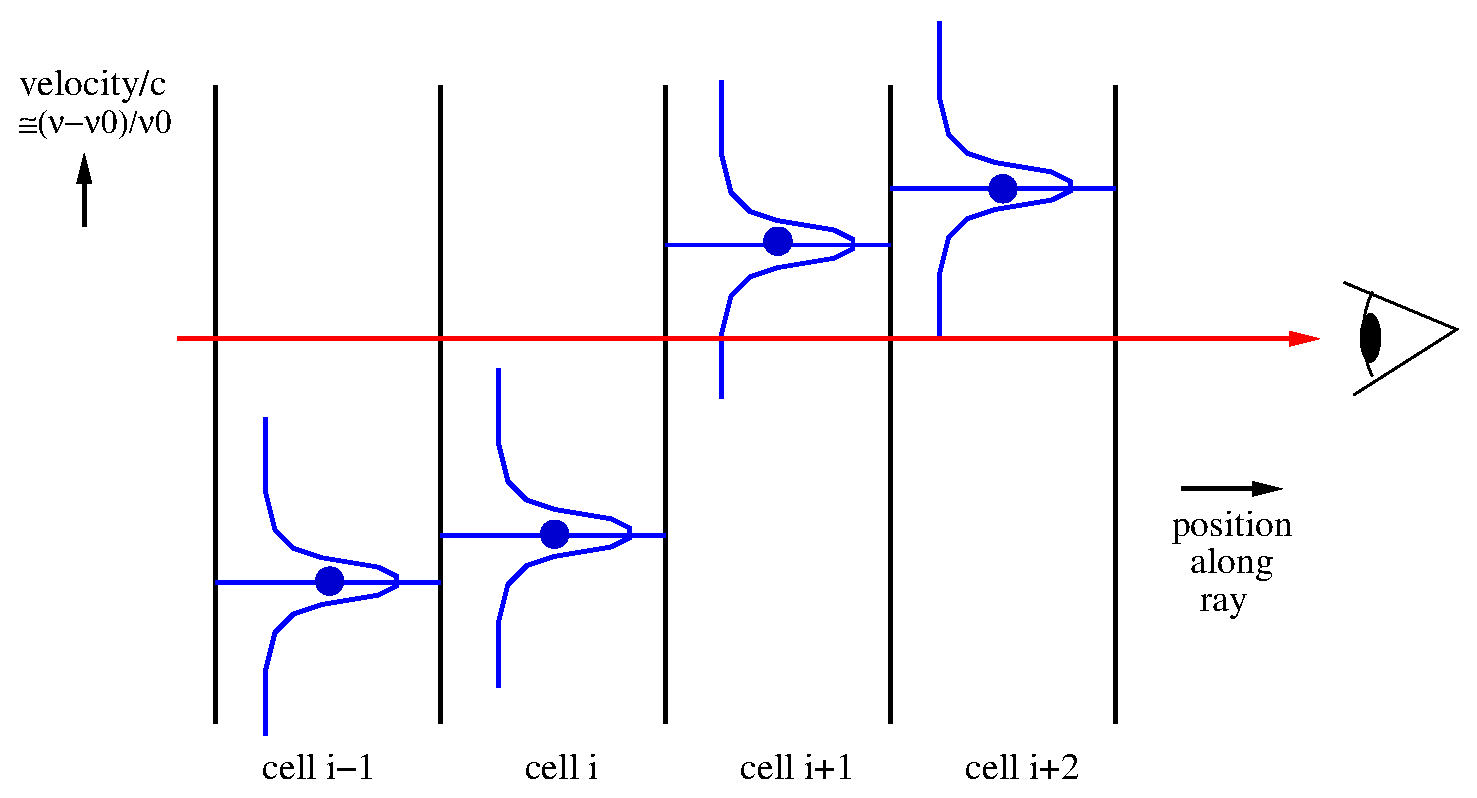
\includegraphics[width=0.45\textwidth]{line_doppjump.eps}
  \hspace{3em}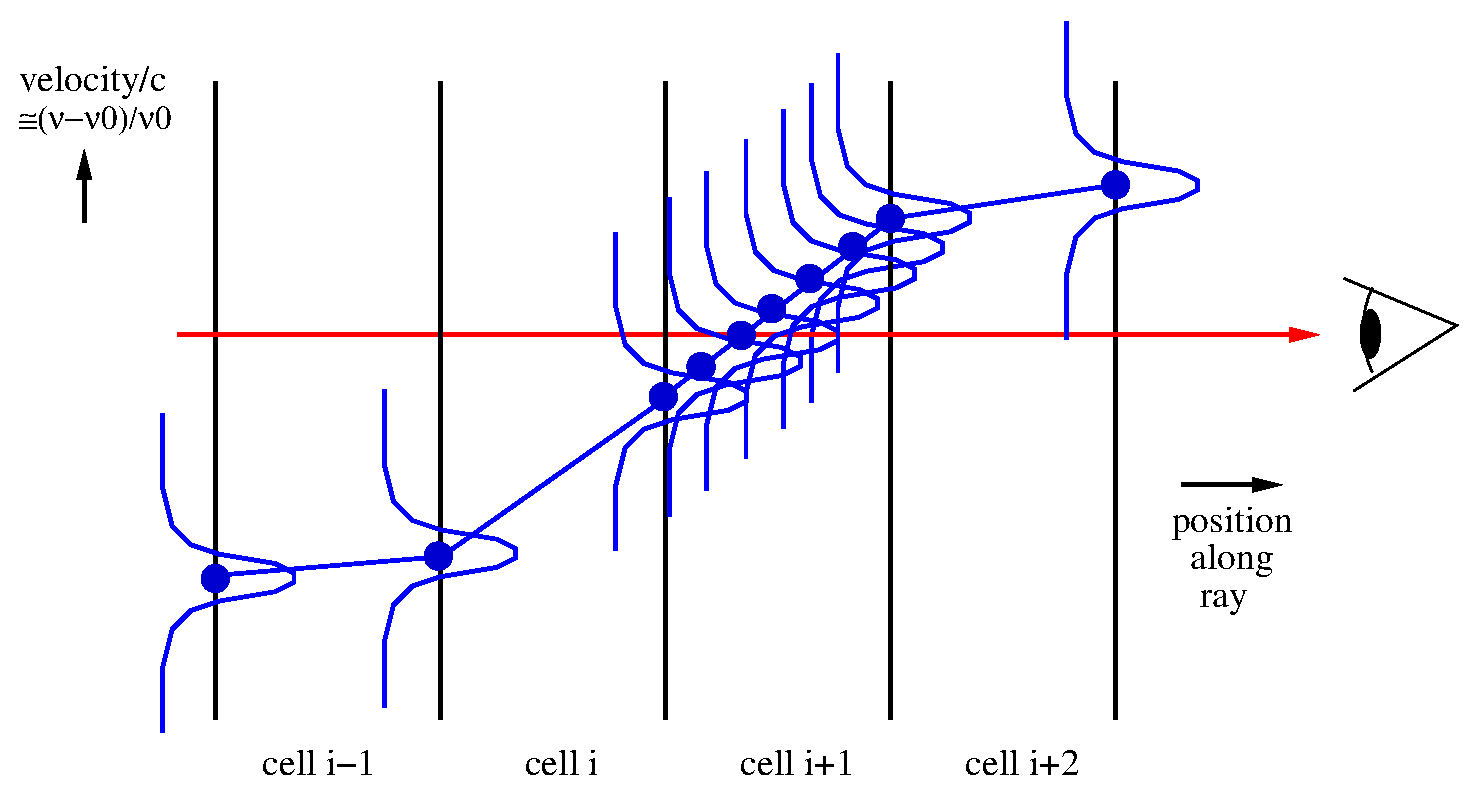
\includegraphics[width=0.45\textwidth]{line_doppcatch.eps}}
\caption{\label{fig-doppler-catch}
Left: Pictographic representation of the doppler jumping problem with 
ray-tracing through a model with strong cell-to-cell velocity differences. 
Right: Pictographic representation of the doppler catching method to 
prevent this problem: First of all, second order integration is done
instead of first order. Secondly, the method automatically detects a
possibly dangerous doppler jump and makes sub-steps to neatly integrate
over the line that shifts in- and out of the wavelength channel of 
interest. 
}
\end{figure}
%
If the local co-moving line width of a line (due to thermal/fundamental
broadning and/or local subgrid ``microturbulence'') is much smaller than the
typical velocity fields in the model, then a dangerous situation can
occur. This can happen if the co-moving line width is narrower than the
doppler shift between two adjacent cells. When a ray is traced, in one cell
the line can then have a doppler shift substantially to the blue of the
wavelength-of-sight, while in the next cell the line suddenly shifted to the
red side. If the intrinsic (= thermal + microturbulent) line width is
smaller than these shifts, neither cell gives a contribution to the emission
in the ray. See Fig.~\ref{fig-doppler-catch}-Left for a pictographic
representation of this problem. In reality the doppler shift between these
two cells would be smooth, and thus the line would smoothly pass over the
wavelength-of-sight, and thus make a contribution. Therefore the numerical
integration may thus go wrong.

The problem is described in more detail in Section
\ref{sec-wavelength-bands}, and one possible solution is proposed there.
But that solution does not always solve the problem.

RADMC-3D has a special method to catch situations like the above, and when
it detects one, to make sub-steps in the integration of the formal transfer
equation so that the smooth passing of the line through the
wavelength-of-sight can be properly accounted for. Here this is called
``doppler catching'', for lack of a better name. The technique was discussed
in great detail in Pontoppidan et al.~(2009, ApJ 704, 1482). The idea is
that the method automatically tests if a line might ``doppler jump'' over
the current wavelength channel. If so, it will insert substeps in the
integration at the location where this danger is present. See
Fig.~\ref{fig-doppler-catch}-Right for a pictographic representation of this
method. Note that this method can only be used with the second order
ray-tracing (see Section \ref{sec-second-order}); in fact, as soon as you
switch the doppler catching on, RADMC-3D will automatically also switch on
the second order ray-tracing.

To switch on doppler catching, you simply add the command-line option 
{\small\tt doppcatch} to the image or spectrum command. For instance:
\begin{asciibox}\begin{verbatim}
radmc3d spectrum iline 1 widthkms 10 doppcatch
\end{verbatim}\end{asciibox}
(again: you do not need to add {\small\tt secondorder}, because
it is automatic when {\small\tt doppcatch} is used). 

The Doppler catching method will assure that the line is integrated over
with small enough steps that it cannot accidently get jumped over. How fine
these steps will be can be adjusted with the {\small\tt
  catch\_doppler\_resolution} keyword in the {\small\tt radmc3d.inp}
file. The default value is 0.2, meaning that it will make the integration
steps small enough that the doppler shift over each step is not more than
0.2 times the local intrinsic (thermal+microturbulent) line width. That is
usually enough, but for some problems it might be important to ensure that
smaller steps are taken. By adding a line
\begin{asciibox}\begin{verbatim}
catch_doppler_resolution = 0.05
\end{verbatim}\end{asciibox}
to the {\small\tt radmc3d.inp} file you will ensure that steps are small
enough that the doppler shift is at most 0.05 times the local line width.

So why is doppler catching an {\em option}, i.e.\ why would this not be
standard?  The reason is that doppler catching requires second order
integration, which requires RADMC-3D to first map all the cell-based
quantities to the cell-corners. This requires extra memory, which for very
large models can be problematic. It also requires more CPU time to calculate
images/spectra with second order integration. So if you do not need it,
i.e.\ if your velocity gradients are not very steep compared to the
intrinsic line width, then it saves time and memory to not use doppler
catching.

It is, however, important to realize that doppler catching is not the golden
bullet. Even with doppler catching it might happen that some line flux is
lost, but this time as a result of too low {\em image resolution}. This is
less likely to happen in problems like ISM turbulence, but it is pretty
likely to happen in models of rotating disks. Suppose we have a very thin
local line width (i.e.\ low gas temperature and no microturbulence) in a
rotating thin disk around a star. In a given velocity channel (i.e.\ at a
given observer-frame frequency) a molecular line in the disk emits only in a
very thin ``ear-shaped'' ring or band in the image. The thinner the
intrinsic line width, the thinner the band on the image. See Pontoppidan et
al.~(2009, ApJ 704, 1482) and Pavlyuchenkov et al.~(2007, ApJ 669, 1262) for
example. If the pixel-resolution of the image is smaller than that of this
band, the image is simply underresolved.  This has nothing to do with the
doppler jumping problem, but can be equally devastating for the results if
the user is unaware of this. There appears to be only one proper solution:
assure that the pixel-resolution of the image is sufficiently fine for the
problem at hand. This is easy to find out: The image would simply look
terribly noisy if the resolution is insufficient. However, if you are not
interested in the images, but only in the spectra, then some amount of
noisiness in the image (i.e.\ marginally sufficient resolution) is OK, since
the total flux is an integral over the entire image, smearing out much of
the noise.  It requires some experimentation, though.

Here are some additional issues to keep in mind:
\begin{itemize}
\item The doppler catching method uses second order integration (see Section
  \ref{sec-second-order}), and therefore all the relevant quantities first
  have to be interpolated from the cell centers to the cell corners. Well
  inside the computational domain this amounts to linear interpolation. But
  at the edges of the domain it would require {\em
    extra}polation\footnote{In 1-D this is more easily illustrated, because
    there the cell corners are in fact cell interfaces. Cells $i$ and $i+1$
    share cell interface $i+1/2$. If we have $N$ cells, i.e.\ cells
    $i=1,\cdots,N$, then we have $N+1$ interfaces, i.e.\ interfaces
    $i=\tfrac{1}{2},\cdots,N+\tfrac{1}{2}$. To get physical quantities from
    the cell centers to cell interfaces
    $i=\tfrac{3}{2},\cdots,N-\tfrac{1}{2}$ requires just interpolation. But
    to find the physical quantities at cell interfaces $i=\tfrac{1}{2}$ and
    $i=N+\tfrac{1}{2}$ one has to extrapolate or simply take the values at
    the cell centers $i=1$ and $i=N$.} RADMC-3D does not do
  extrapolation but simply takes the average values of the nearest
  cells. Also the gas velocity is treated like this. This means that over
  the edge cells the gradient in the gas velocity tends to be (near)
  0. Since for the doppler catching it is the gradient of the velocity that
  matters, this might yield some artifacts in the spectrum if the density in
  the border cells is high enough to produce substantial line
  emission. Avoiding this numerical artifact is relatively easy: One should
  then simply put the number density of the molecule in question to zero in
  the boundary cells.
\item If you are using RADMC-3D on a 3-D (M)HD model which has strong shocks
  in its domain, then one must be careful that (magneto-)hydrodynamic codes
  tend to smear out the shock a bit. This means that there will be some
  cells that have intermediate density and velocity in the smeared out
  region of the shock. This is unphysical, but an intrinsic numerical
  artifact of numerical hydrodynamics codes. This might, under some
  conditions, lead to unphysical signal in the spectrum, because there would
  be cells at densities, temperatures and velocities that would be in
  between the values at both sides of the shock and would, in reality, not
  be there. It is very difficult to avoid this problem, and even to find out
  if this problem is occurring and by how much. One must simply be very
  careful of models containing strong shocks and do lots of testing.  One
  way to test is to use the doppler catching method and vary the doppler
  catching resolution (using the {\small\tt catch\_doppler\_resolution}
  keyword in {\small\tt radmc3d.inp}).
\item If using line transfer in spherical coordinates using doppler
  catching, the linear interpolation of the line shift between the beginning
  and the end of a segment may not always be enough to accurately prevent
  doppler jumps. This is because in addition to the physical gradient of gas
  velocity, the projected gas velocity along a ray changes also along the
  ray due to the geometry (the use of spherical coordinates). Example: a
  spherically symmetric radially outflowing wind with constant outward
  velocity $v_r=$const. Although $v_r$ is constant, the 3-D {\em vector}
  $\vec v$ is not constant, since it always points outward. A ray through
  this wind will thus have a varying $\vec n\cdot \vec v$ along the ray.  In
  the cell where the ray reaches its closest approach to the origin of the
  coordinate system the $\vec n\cdot \vec v$ will vary the strongest.  This
  may be such a strong effect that it could affect the reliability of the
  code. {\em As of version 0.41 of this code a method is in place to prevent
    this}. It is switched on by default, but it can be switched off manually
  for testing purposes. See Section \ref{sec-secord-spher} for details.
\end{itemize}


\section{Background information: Calculation and storage of level populations}
\label{sec-calcstore-levpop}
%
If RADMC-3D makes an image or a spectrum with molecular (or atomic) lines
included, then the level populations of the molecules/atoms have to be
computed. In the standard method of ray-tracing of images or spectra, these
level populations are first calculated in each grid cell and stored in a
global array. Then the raytracer will render the image or spectrum. 

The storage of the level populations is a tricky matter, because if this is
done in the obvious manner, it might require a huge amount of memory. This
would then prevent us from making large scale models. For instance: if you
have a molecule with 100 levels in a model with 256x256x256 $\simeq
1.7\times 10^7$ cells, the global storage for the populations alone (with
each number in double precision) would be roughly 100x8x256x256x256 $\simeq$
13 Gigabyte.

However, if you intend to make a spectrum in just 1 line, you do not need
all these level populations. To stick to the above example, let us take the
CO 1-0 line, which is then line 1 and which connects levels $J=1$ and $J=0$,
which are levels 2 and 1 in the code (if you use the Leiden database CO data
file).  Once the populations have been computed, we only need to store the
levels 1 and 2. This would then require 2x8x256x256x256 $\simeq$ 0.26
Gigabyte, which would be {\em much} less memory-costly.

As of version 0.29 RADMC-3D automatically figures out which levels have to
be stored in a global array, in order to be able to render the images or the
spectrum properly. RADMC-3D will go through all the lines of all molecules
and checks if they contribute to the wavelength(s), of the image(s) or the
spectrum. Once it has assembled a list of ``active'' lines, it will make a
list of ``active'' levels that belong to these lines. It will then declare
this to be the ``subset'' of levels for which the populations will be stored
globally.

In other words: RADMC-3D now takes care of the memory-saving storage of
the populations automatically.

{\em How does RADMC-3D decide whether a line contributes to some wavelength
  $\lambda$?} A line $i$ with line center $\lambda_i$ is considered to
contribute to an image at wavelength $\lambda$ if 
\begin{equation}
| \lambda_i-\lambda | \le C_{\mathrm{margin}}\Delta\lambda_i
\end{equation}
where $\Delta\lambda_i$ is the line width (including all contributions) and
$C_{\mathrm{margin}}$ is a constant. By default
\begin{equation}
C_{\mathrm{margin}} = 12
\end{equation}
But you can change this to another value, say 24, by adding in the
{\small\tt radmc3d.inp} file a line containing, e.g.\ {\small\tt
  lines\_widthmargin = 24}.

Note that if you use RADMC-3D as a child process (e.g.\ with the {\small\tt
  viewimage.pro} widget; see Chapters \ref{chap-child-mode} and
\ref{chap-idl-analysis-tools}), then RADMC-3D will re-use the calculated
populations for further images/spectra, if those new images/spectra contain
the same lines as the previous image/spectrum. That could save time.
Example: You start {\small\tt viewimage.pro} and you get an image at some
standard wavelength at first. You select a wavelength right at line center
for the CO 2-1 transition (i.e.\ in the code this is from level nr 3 to 2)
and make a new image. RADMC-3D now notices that it will need to calculate
and store the populations for levels 2 and 3, it allocates an array for two
levels, it computes the populations for levels 2 and 3 and stores these into
the global array. Then it will raytrace the image. Now, if you now change
the orientation of the object (e.g.\ by changing the inclination, for
instance), then it will skip the level population calculation because it
recognizes that it has them already available. If you now change the
wavelength a bit (by, say, 2 km/s), it will also re-use the populations. But
if you now change the wavelength to the 1-0 transition, it will deallocate
the current array, create a brand new array and recalculate the populations.

You can in fact get a dump of the level populations that have been computed
and used for the image(s)/spectrum you created, by adding {\small\tt 
writepop} on the command line. Example:
\begin{asciibox}\begin{verbatim}
radmc3d spectrum iline 1 widthkms 10 writepop
\end{verbatim}\end{asciibox}
This then creates (in addition to the spectrum) a file called (for our
example of the CO molecule) {\small\tt levelpop\_co.dat}. In the IDL file
{\small\tt readradmc.pro} there is a subroutine called {\small\tt
  read\_levelpop()} that can read the data from {\small\tt levelpop\_co.dat}
into IDL for visualization. You will then find that indeed only the
necessary levels have been used.

If, for some reason, you want always {\em all} levels to be stored (and you
can afford to do so with the size of your computer's memory), you can make
RADMC-3D do so by adding {\small\tt noautosubset} as a keyword to the
command line, or by adding {\small\tt lines\_autosubset = 0} to the
{\small\tt radmc3d.inp} file. However, for other than code testing purposes,
it seems unlikely you will wish to do this.

\section{In case it is necessary: On-the-fly calculation of populations}
\label{sec-onthefly}
%
There might be rare circumstances in which you do not want to have to store
the level populations in a global array. For example: you are making a spectrum
of the CO bandhead, in which case you have many tens of lines in a single
spectrum. If your model contains 256x256x256 cells (see example in Section
\ref{sec-calcstore-levpop}) then this might easily require many Gigabytes of
memory just to store the populations. 

For the LTE, LVG and optically thin level population modes there is a way
out: You can force RADMC-3D to compute the populations {\em on-the-fly}
during the ray-tracing, which does not require a global storage of the
level populations. 

The way to do this is simple: Just make the {\small\tt lines\_mode}
negative. So for on-the-fly LTE mode use {\small\tt lines\_mode=-1}, for
on-the-fly user-defined populations mode use {\small\tt lines\_mode=-2}, for
on-the-fly LVG mode use {\small\tt lines\_mode=-3} and for on-the-fly
optically thin populations use {\small\tt lines\_mode=-4}.

{\em NOTE: The drawback of this method is that, under certain circumstances,
  it can slow down the code dramatically.} This slow-down happens if you use
e.g.\ second-order integration (Section \ref{sec-second-order}) and/or
doppler catching (Section \ref{sec-doppler-catching}) together with
non-trivial population solving methods like LVG. So please use the
on-the-fly method only when you are forced to do so (for memory reasons).


\section{For experts: Selecting a subset of lines and levels ``manually''}
\label{sec-line-selection}
%
As explained in Section \ref{sec-calcstore-levpop}, RADMC-3D automatically
makes a selection of levels for which it will allocate memory for the global
level population storage. 

If, for some reason, you wish to make this selection yourself ``by hand'',
this can also be done. However, please be informed that there are very
few circumstances under which you may want to do this. The automatic
subset selection of RADMC-3D is usually sufficient!

{\em If} you decided to really want to do this, here is how:
\begin{enumerate}
\item Switch off the automatic subset selection by adding {\small\tt
    noautosubset} as a keyword to the command line, or by adding {\small\tt
    lines\_autosubset = 0} to the {\small\tt radmc3d.inp} file.
\item In the {\small\tt lines.inp} file, for each molecule, modify the
  '0 0' (the first two zeroes after 'leiden') in the way described below.
\end{enumerate}

In Section \ref{sec-line-dot-inp} you can see that each molecule has a line
like:
\begin{asciibox}\begin{verbatim}
co   leiden   0  0  0
\end{verbatim}\end{asciibox}
or so (here for the example of CO). In Section \ref{sec-line-dot-inp} we
explained the meaning of the third number, but we did not explain the
meaning of the first and second ones. These are meant for this subset
selection. If we want to store only the first 10 levels of the CO 
molecule, then replace the above line with:
\begin{asciibox}\begin{verbatim}
co   leiden   0  10  0
\end{verbatim}\end{asciibox}
If you want to select specific levels (let us choose the {\small\tt
  ilevel=3} and {\small\tt ilevel=4} levels of the above example),
then write:
\begin{asciibox}\begin{verbatim}
co   leiden   1  2  0
3 4
\end{verbatim}\end{asciibox}
The `1' says that a list of levels follows, the `2' says that two levels
will be selected and the next line with `3' and `4' say that levels 3
and 4 should be selected. 




%----------------------------------------------------------------------------
%               CHAPTER: GAS CONTINUUM OPACITIES
%----------------------------------------------------------------------------
\chapter{Gas continuum opacities and emissivities}
\label{chap-gas-continuum}
%
In addition to dust and line radiative transfer, RADMC-3D can also handle
gas continuum opacities. Here is a list of features that are now already
working, marked with [+], and those which are not yet (!!) built in,
marked with [-]. Those that are currently being developed are marked with
[.] and those that are ready, but are still in the testing phase are marked
with [t].
\begin{itemize}
\item[] The following processes are included:
  \begin{itemize}
  \item[][t] Gas free-free absorption/emission
  \item[][.] Gas bound-free absorption/emission
  \end{itemize}
\item[][.] Self-consistent determination of the gas temperature, based
  on the continuum opacity and possibly also the lines. Perhaps also 
  various non-thermal heating processes (photoelectric heating etc) will
  be included. But this is future work.
\end{itemize}


\section{Gas continuum opacities and emissivities}
While under most circumstances gas emission is mostly in the form of 
lines, there are also continuum sources of emission and opacity. 
Gas continuum opacities can be included in a way very similar to the dust
opacities.  Since currently we envisage thermalized gas (i.e.\ no
accelerated particle distributions, for instance), we can then use
Kirchhoff's law to compute, with the gas temperature, the
emissivities. Normally the user will have to determine all the locally
required quantities, including the gas temperature, the ion and/or electron
density etc. In the first version(s) of this module the gas temperature will
not be computed self-consistently, but instead have to be given by the user.
The processes will be discussed one-by-one below. 

Each process can be switched on or off independently:\\
\begin{tabular}{llll}
Process:  &  Command-line switch on & Command-line switch off & {\small\tt radmc3d.inp} variable (0/1) \\
\hline
All processes     & {\small\tt inclgascont} & {\small\tt nogascont} & {\small\tt incl\_gascont} \\
Thermal free-free & {\small\tt inclfreefree} & {\small\tt nofreefree} & {\small\tt incl\_freefree} \\
\end{tabular}

The main switch is the {\small\tt incl\_gascont}. If this is 0, all gas
continuum processes are switched off. If it is 1, then gas continuum
processes that have their own switch on will be included. Typically, by
switching on one of the processes, the main switch will also be automatically
switched on. But the reverse is not true: if you switch off one of the
processes, the main switch remains on. 


\subsection{Thermal free-free emission/absorption}
The process of thermal free-free emission and absorption is given by the
following formula (Eq.\ 2.96 of Gordon \& Sorochenko, 2002, Kluwer Academic
Publishers):
\begin{equation}
\alpha_\nu^{\mathrm{ff}} = 0.2120 \frac{N_e N_i}{\nu^{2.1} T^{1.35}}
\end{equation}
in units of cm$^{-1}$ (i.e.\ the mean free photon path is
$1/\alpha_\nu^{\mathrm{ff}}$).

This mode requires the {\small electron\_numdens(:)}, {\small
  ion\_numdens(:)}, and {\small gastemp(:)} arrays to be set. This is
typically done by providing the files {\small electron\_numdens.inp},
{\small ion\_numdens.inp} and {\small gas\_temperature.inp} (see Chapter
\ref{chap-input-files}), or by allocating and setting the arrays directly in
the {\small\tt userdef\_module.f90}.






\section{Self-consistent gas temperature iteration}
In future versions of RADMC-3D the gas temperature can, like the dust
temperature, be determined through a Monte Carlo procedure. In contrast
to the dust, however, the gas opacities change with temperature. The
Monte Carlo simulation must therefore be repeated a few times to converge
on the right temperatures. 

At the moment this method is, however, not yet implemented. Instead, the gas
temperature must be set by the user, either in the form of a file called
{\small\tt gas\_temperature.inp} or in the {\small\tt userdef\_module.f90}
module.






%----------------------------------------------------------------------------
%               CHAPTER: MAKING IMAGES AND SPECTRA
%----------------------------------------------------------------------------
\chapter{Making images and spectra}
\label{chap-images-spectra}
%
Much has already been said about images and spectra in the chapters on
dust radiative transfer and line radiative transfer. But here we will
combine all this and go deeper into this material. So presumably you
do not need to read this chapter if you are a beginning user. But for
more sophisticated users (or as a reference manual) this chapter may
be useful and presents many new features and more in-depth insight.

\section{Basics of image making with RADMC-3D}
\label{sec-images}
%
Images and spectra are typically made after the dust temperature has been
determined using the thermal Monte Carlo run (see Chapter \ref{chap-dust-transfer}). An image can now be made with a simple call to
{\small\tt radmc3d}\footnote{Please also read Section \ref{sec-idl-makeimage} for IDL routines that do all of this for you
  conveniently. The choice is up to you: you can either do this directly as
  described here, or use the IDL routines.}:
\begin{asciibox}\begin{verbatim}
radmc3d image lambda 10
\end{verbatim}\end{asciibox}
This makes an image of the model at wavelength $\lambda=10\mu$m and writes
this to the file {\small\tt image.out}. We refer to Section
\ref{sec-image-out} for details of this file and how to interpret the
content. See Chapter \ref{chap-idl-analysis-tools} for an extensive IDL tool
set that make it easy to read and handle these files. The vantage point is
at infinity at a default inclination of 0, i.e.\ pole-on view. You can
change the vantage point:
\begin{asciibox}\begin{verbatim}
radmc3d image lambda 10 incl 80 phi 30
\end{verbatim}\end{asciibox}
which now makes the image at inclination 80 degrees away from the z-axis
(i.e.\ almost edge-on with respect to the x-y plane), and rotates the
location of the observer by 30 degrees clockwise around the
z-axis\footnote{Here clockwise is defined with the z-axis pointing toward
  you.} (i.e.\ with respect to the observer the model is rotated
counter-clockwise around the z-axis by 30 degrees). 
%
\begin{figure}
\centerline{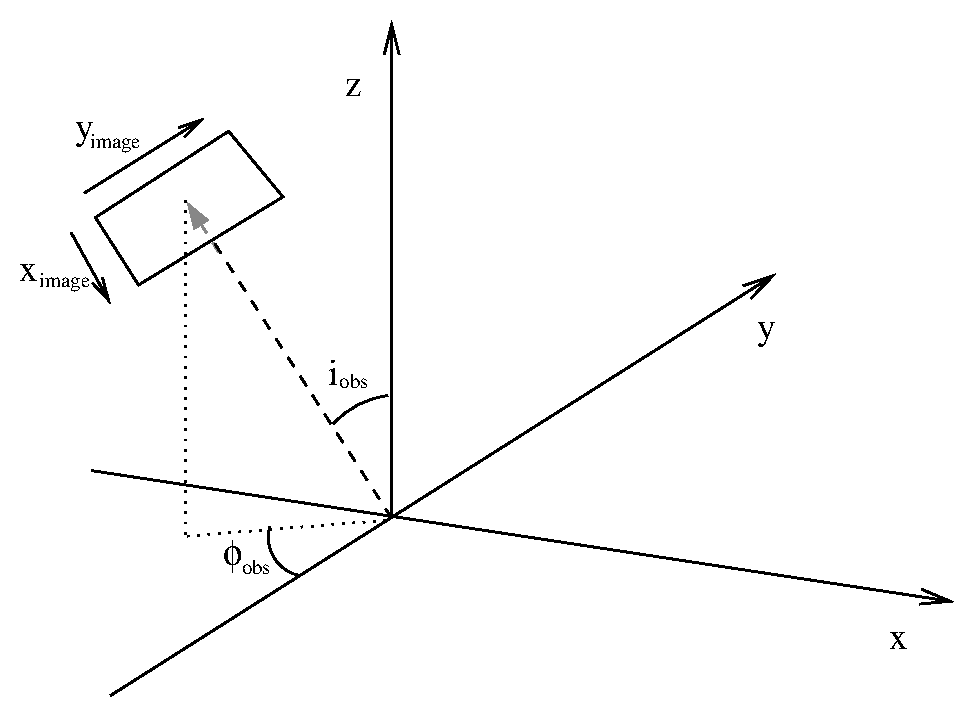
\includegraphics[width=0.45\textwidth]{camera_orient.eps}
  \hspace{3em}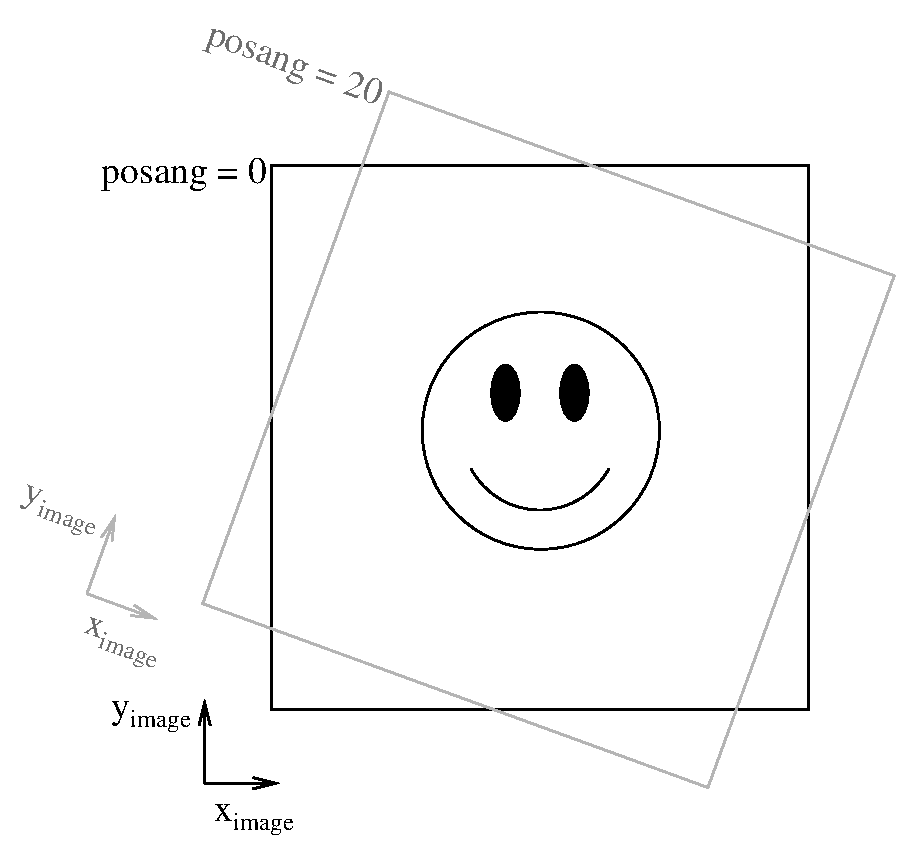
\includegraphics[width=0.38\textwidth]{posang.eps}}
\caption{\label{fig-cameraorient}
%
Figure depicting how the angles ``incl'', ``phi'' and ``posang'' orient
the camera for images and spectra made with RADMC-3D. The code uses a right-handed
coordinate system. The left figure shows from which direction the observer
is looking at the system, where $i_{\mathrm{obs}}$ is the ``incl'' keyword
and $\phi_{\mathrm{obs}}$ is the ``phi'' keyword. The $x_{\mathrm{image}}$ and
$y_{\mathrm{image}}$ are the horizontal (left-to-right) and vertical (bottom-to-top)
coordinates of the image. For $i_{\mathrm{obs}}=0$ and $\phi_{\mathrm{obs}}=0$
the $x_{\mathrm{image}}$ aligns with the 3-D $x$-coordinate and 
$y_{\mathrm{image}}$ aligns with the 3-D $y$-coordinate. The right figure shows
the way the camera can be rotated in the image plane using ``posang''. Positive
``posang'' means that the camera is rotated clockwise, so the object shown
is rotated counter-clockwise with respect to the image coordinates.
%
}
\end{figure}
%
You can also rotate the
camera in the image plane with
\begin{asciibox}\begin{verbatim}
radmc3d image lambda 10 incl 45 phi 30 posang 20
\end{verbatim}\end{asciibox}
which rotates the camera by 20 degrees clockwise (i.e.\ the image rotates
counter-clockwise). Figure \ref{fig-cameraorient} shows the definitions of
all three angles. Up to now the camera always pointed to one single point
in space: the point (0,0,0). You can change this:
\begin{asciibox}\begin{verbatim}
radmc3d image lambda 10 incl 45 phi 30 posang 20 pointau 3.2 0.1 0.4
\end{verbatim}\end{asciibox}
which now points the camera at the point (3.2,0.1,0.4), where the numbers
are in units of AU. The same can be done in units of parsec:
\begin{asciibox}\begin{verbatim}
radmc3d image lambda 10 incl 45 phi 30 posang 20 pointpc 3.2 0.1 0.4
\end{verbatim}\end{asciibox}
Note that {\small\tt pointau} and {\small\tt pointpc} are always 3-D
positions specified in cartesian coordinates. This remains also true when
the model-grid is in spherical coordinates and/or when the model is 2-D
(axisymmetric) or 1-D (spherically symmetric): 3-D positions are always
specified in x,y,z. 

Let's now drop the pointing again, and also forget about the {\small\tt
  posang}, and try to change the number of pixels used:
\begin{asciibox}\begin{verbatim}
radmc3d image lambda 10 incl 45 phi 30 npix 100
\end{verbatim}\end{asciibox}
This will make an image of 100x100. You can also specify the x- and y- 
direction number of pixels separately:
\begin{asciibox}\begin{verbatim}
radmc3d image lambda 10 incl 45 phi 30 npixx 100 npixy 30
\end{verbatim}\end{asciibox}
Now let's forget again about the number of pixels and change the size of the
image, i.e.\ which zooming factor we have:
\begin{asciibox}\begin{verbatim}
radmc3d image lambda 10 incl 45 phi 30 sizeau 30
\end{verbatim}\end{asciibox}
This makes an image which has 30 AU width and 30 AU height (i.e.\ 15 AU
from the center in both directions). Same can be done in units of parsec
\begin{asciibox}\begin{verbatim}
radmc3d image lambda 10 incl 45 phi 30 sizepc 30
\end{verbatim}\end{asciibox}
Although strictly speaking redundant is the possibility to zoom-in right
into a selected box in this image:
\begin{asciibox}\begin{verbatim}
radmc3d image lambda 10 incl 45 phi 30 zoomau -10 -4. 0 6
\end{verbatim}\end{asciibox}
which means that we zoom in to the box given by $-10\le x\le-4$ AU and $0\le
y\le 6$ AU on the original image (note that {\small\tt zoomau -15 15 -15 15}
gives the identical result as {\small\tt sizeau 30}). This possibility is
strictly speaking redundant, because you could also change the {\small\tt
  pointau} and {\small\tt sizeau} to achieve the same effect (unless you
want to make a non-square image, in which case this is the only way). But it
is just more convenient to do any zooming-in this way. Please note that when
you make non-square images with {\small\tt zoomau} or {\small\tt zoompc},
the code will automatically try to keep the pixels square in shape by
adapting the number of pixels in x- or y- direction in the image and
adjusting one of the sizes a tiny bit to assure that both x- and y- size are
an integer times the pixel size. These are very small adjustments (and only
take place for non-square zoom-ins).  If you want to force the code to take
{\em exactly} the zoom area, and you don't care that the pixels then become
slightly non-square, you can force it with {\small\tt truezoom}:
\begin{asciibox}\begin{verbatim}
radmc3d image lambda 10 incl 45 phi 30 sizeau 30 zoomau -10 -4. 0 3.1415 truezoom
\end{verbatim}\end{asciibox}
If you do not want the code to adjust the number of pixels in x- and y-
direction in its attempt to keep the pixels square:
\begin{asciibox}\begin{verbatim}
radmc3d image lambda 10 incl 45 phi 30 sizeau 30 zoomau -10 -4. 0 3.1415 npixx 100 npixy 4 truepix
\end{verbatim}\end{asciibox}

Now here are some special things. Sometimes you would like to see an image
of just the dust, not including stars (for stars in the image: see Section
\ref{sec-image-stars}). So blend out the stars in the image, you use the
{\small\tt nostar} option:
\begin{asciibox}\begin{verbatim}
radmc3d image lambda 10 incl 45 phi 30 nostar
\end{verbatim}\end{asciibox}

Another special option is to get a `quick image', in which the code does not
attempt assure flux conservation in the image (see Section
\ref{sec-image-refinement} for the issue of flux conservation). Doing the
image with flux conservation is slower than if you make it without flux
conservation. Making an image without flux conservation can be useful if you
want to have a `quick look', but is strongly discouraged for actual
scientific use. But for a quick look you can do:
\begin{asciibox}\begin{verbatim}
radmc3d image lambda 10 incl 45 phi 30 nofluxcons
\end{verbatim}\end{asciibox}
Note: In the IDL widget interface {\small\tt viewimage.pro} the default
is to use this `quick look' option, because you typically want to make
images quickly if you use the {\small\tt viewimage.pro} interface. But
there is a button (called ``preview'') that if you unclick it, it will
do flux-conserving imaging. 

If you want to produce images with a smoother look (and which
also are more accurate), you can ask RADMC-3D to use second order 
integration for the images: 
\begin{asciibox}\begin{verbatim}
radmc3d image lambda 10 incl 45 phi 30 secondorder
\end{verbatim}\end{asciibox}
NOTE: The resulting intensities may be slightly different from the case
when first order integration (default) is used, in particular if the 
grid is somewhat course and the objects of interest are optically thick. 
Please consult Section \ref{sec-second-order} for more information.

{\em Important for polarized radiative transfer:} If you use polarized
scattering, then you may want to creat images with polarization 
information in them. You have to tell RADMC-3D to do this by adding
{\small\tt stokes} to the command line:
\begin{asciibox}\begin{verbatim}
radmc3d image lambda 10 incl 45 phi 30 stokes
\end{verbatim}\end{asciibox}
The definitions of the Stokes parameters (orientation etc) can be
found in Section \ref{sec-definitions-stokes} and the format of
{\small\tt image.out} in this case can be found in Section 
\ref{sec-image-out}.

Note: All the above commands call {\small\tt radmc3d} separately. If it
needs to load a large model (i.e.\ a model with many cells), then the 
loading may take a long time. If you want to make many images in a row,
this may take too much time. Then it is better to call {\small\tt radmc3d}
as a child process and pass the above commands through the biway pipe
(see Chapter \ref{chap-child-mode}).


\section{Making multi-wavelength images}
\label{sec-multi-wavelength-images}
%
Sometimes you want to have an image of an object at multiple wavelength
simultaneously. Rather than calling RADMC-3D separately to make an image for
each wavelength, you can make all images in one command. The only thing you
have to do is to tell RADMC-3D which wavelengths it should take. There are
various different ways you can tell RADMC-3D what wavelengths to take. This
is described in detail in Section \ref{sec-set-camera-frequencies}. Here
we will focus as an example on just one of these methods. Type, for instance,
\begin{asciibox}\begin{verbatim}
radmc3d image incl 45 phi 30 lambdarange 5. 20. nlam 10
\end{verbatim}\end{asciibox}
This will create 10 images at once, all with the same viewing perspective,
but at 10 wavelengths regularly distributed between 5 $\mu$m and 20 $\mu$m.
All images are written into a single file, {\small\tt image.out}
(See Section \ref{sec-image-out} for its format). 

In IDL you simply type:
\begin{asciibox}\begin{verbatim}
.r readradmc
a=readimage()
\end{verbatim}\end{asciibox}
and you will get all images at once. To plot one of them:
\begin{asciibox}\begin{verbatim}
plotimage,a,ilam=3
\end{verbatim}\end{asciibox}
which will plot image number 3 (out of images number 0 to 9). To find out
which wavelength this image is at:
\begin{asciibox}\begin{verbatim}
print,a.lambda[3]
\end{verbatim}\end{asciibox}
which will return 7.9370053 in this example.

Note that all of the commands in Section \ref{sec-images} are of course also
applicable to multi-wavelength images, except for the {\small\tt lambda}
keyword, as this conflicts with the other method(s) of specifying the
wavlengths of the images. Now please turn to Section
\ref{sec-set-camera-frequencies} for more information on how to specify
the wavelengths for the multiple wavelength images.


\section{Making spectra}
\label{sec-making-spectra}
%
The standard way of making a spectrum with {\small\tt radmc3d} is in fact
identical to making 100x100 pixel images with flux conservation (i.e.\ recursive
sub-pixeling, see Section \ref{sec-image-refinement}) at multiple
frequencies. You can ask {\small\tt radmc3d} to make a {\em spectral energy
  distribution (SED)} with the command
\begin{asciibox}\begin{verbatim}
radmc3d sed incl 45 phi 30
\end{verbatim}\end{asciibox}
This will put the observer at inclination 45 degrees and angle phi 30
degrees, and make a spectrum with wavelength points equal to those listed
in the {\small\tt wavelength\_micron.inp} file. 

The output will be a file called {\small\tt spectrum.out} (see Section
\ref{sec-output-spectrum-out}). In Section \ref{sec-spectra-from-idl} it is
discussed how to read this file into IDL.

You can also make a spectrum on a set of wavelength points of your own
choice. There are multiple ways by which you can specify the set of
frequencies/wavelength points for which to make the spectrum: they are
described in Section \ref{sec-set-camera-frequencies}. If you have made
your selection in such a way, you can make the spectrum at this wavelength
grid by 
\begin{asciibox}\begin{verbatim}
radmc3d spectrum incl 45 phi 30 <COMMANDS FOR WAVELENGTH SELECTION>
\end{verbatim}\end{asciibox}
where the last stuff is telling {\small\tt radmc3d} how to select the
wavelengths (Section \ref{sec-set-camera-frequencies}). An example:
\begin{asciibox}\begin{verbatim}
radmc3d spectrum incl 45 phi 30 lambdarange 5. 20. nlam 100
\end{verbatim}\end{asciibox}
will make a spectrum with a regular wavelength grid between 5 and 20 $\mu$m
and 100 wavelength points. But see Section \ref{sec-set-camera-frequencies}
for more details and options.

The output file {\small\tt spectrum.out} will have the same format as
for the {\small\tt sed} command.

Making a spectrum can take RADMC-3D some time, especially in the default
mode, because it will do its best to shoot its rays to pick up all cells of
the model (see Section \ref{sec-recursive-subpixeling}). In particularly
in spherical coordinates RADMC-3D can be perhaps {\em too} conservative (and
thus slow). For spherical coordinates there are ways to tell RADMC-3D to be
somewhat less careful (and thereby faster): see Section
\ref{sec-rec-subpixel-spher-coord}.

Note that you can adjust the fine-ness of the images from which the
spectrum is calculated using {\small\tt npix}:
\begin{asciibox}\begin{verbatim}
radmc3d sed incl 45 phi 30 npix 2
\end{verbatim}\end{asciibox}
What this does is use a 2x2 pixel image instead of a 100x100 pixel image as
the starting resolution. Of course, if it would really be just a 2x2 pixel
image, the flux would be entirely unreliable and useless. However, using the
above mentioned ``sub-pixeling'' (see Section
\ref{sec-recursive-subpixeling}) it will automatically try to recursively
refine these pixels until the required level of refinement is reached. So
under normal circumstances even npix=2 is enough, and in earlier versions of
RADMC-3D this 2x2 top-level image resolution was in fact used as a starting
point. But for safety reasons this has now been changed to the standard
100x100 resolution which is also the default for normal images. If 100x100
is not enough, try e.g.:
\begin{asciibox}\begin{verbatim}
radmc3d sed incl 45 phi 30 npix 400
\end{verbatim}\end{asciibox}
which may require some patience.


\subsection{What is ``in the beam'' when the spectrum is made?}
As mentioned above, a spectrum is simply made by making a rectangular image
at all the wavelengths points, and integrating over these images. The
resulting fluxes at each wavelength point is then the spectral flux at that
wavelength point. This means that the integration area of flux for the
spectrum is (a) rectangular and (b) of the same size at all wavelengths.

So, what {\em is} the size of the image that is integrated over? The answer
is: it is the same size as the default size of an image. In fact, if you
make a spectrum with
\begin{asciibox}\begin{verbatim}
radmc3d spectrum incl 45 phi 30 lambdarange 5. 20. nlam 10
\end{verbatim}\end{asciibox}
then this is the same as if you would type
\begin{asciibox}\begin{verbatim}
radmc3d image incl 45 phi 30 lambdarange 5. 20. nlam 10
\end{verbatim}\end{asciibox}
and read in the file {\small\tt image.out} in into IDL (see Section
\ref{sec-multi-wavelength-images}) or your favorite other data language, and
integrate the images to obtain fluxes. In other words: the command
{\small\tt spectrum} is effectively the same as the command {\small\tt
image} but then instead of writing out an {\small\tt image.out} file, it
will integrate over all images and write a {\small\tt spectrum.out} file.

If you want to have a quick look at the area over which the spectrum is
to be computed, but you don't want to compute all the images, just type
e.g.:
\begin{asciibox}\begin{verbatim}
radmc3d image lambda 10 incl 45 phi 30
\end{verbatim}\end{asciibox}
then you see an image of your source at $\lambda=10\mu$m, and the
integration area is precisely this area -- at all wavelengths. Like with
the images, you can specify your viewing area, and thus your integration
area. For instance, by typing
\begin{asciibox}\begin{verbatim}
radmc3d image lambda 10 incl 45 phi 30 zoomau -2 -1 -0.5 0.5
\end{verbatim}\end{asciibox}
makes an image of your source at $\lambda=10\mu$m at inclination 45 degrees,
and orientation 30 degrees, and zooms in at an are from -2 AU to -1 AU
in x-direction (in the image) and from -0.5 AU to 0.5 AU in y-direction 
(in the image). To make an SED within the same integration area:
\begin{asciibox}\begin{verbatim}
radmc3d sed incl 45 phi 30 zoomau -2 -1 -0.5 0.5
\end{verbatim}\end{asciibox}
In this case we have an SED with a ``beam size'' of 1 AU diameter, but
keep in mind that the ``beam'' is square, not circular. 


\subsection{Can one specify more realistic ``beams''?}
\label{sec-aperture}
%
Clearly, a wavelength-independent beam size is unrealistic, and also the
square beam is unrealistic. So is there a way to do this better? In
reality one should really know exactly how the object is observed and
how the flux is measured. If you use an interferometer, for instance,
maybe your flux is meant to be the flux in a single synthesized beam.
For a spectrum obtained with a slit, the precise flux is dependent on
the slit width: the wider the slit, the more signal you pick up, but
it is a signal from a larger area. 

So if you really want to be sure that you know exactly what you are doing,
then the best method is to do this youself by hand. You make
multi-wavelength images:
\begin{asciibox}\begin{verbatim}
radmc3d image incl 45 phi 30 lambdarange 5. 20. nlam 10
\end{verbatim}\end{asciibox}
and integrate over the images in the way you think best mimics the actual
observing procedure. You can do so, for instance, in IDL.  See Section
\ref{sec-multi-wavelength-images} for more information about
multi-wavelength images.

But to get some reasonable estimate of the effect of the
wavelength-dependent size and circular geometry of a ``beam'', RADMC-3D
allows you to make spectra with a simplistic circular mask, the radius of
which can be specified as a function of wavelength in the file {\small\tt
  aperture\_info.inp} (see Section \ref{sec-aperture-info-file}).  This file
should contain a table of mask radii at various wavelengths, and when making
a spectrum with the command-line keyword {\small\tt useapert} the mask radii
will be found from this table by interpolation. In other words: the
wavelength points of the {\small\tt aperture\_info.inp} file do not have to
be the same as those used for the spectrum. But their range {\em must} be
larger or equal than the range of the wavelengths used for the spectrum,
because otherwise interpolation does not work. In the most extreme
simplistic case the {\small\tt aperture\_info.inp} file contains merely two
values: one for a very short wavelength (shorter than used in the spectrum)
and one for a very long wavelength (longer than used in the spectrum). The
interpolation is then done double-logarithmically, so that a powerlaw is
used between sampling points. So if you use a telescope with a given
diameter for the entire range of the spectrum, two sampling points would
indeed suffice.

You can now make the spectrum with the aperture in the following way:
{\small\begin{verbatim}
radmc3d sed useapert dpc 100
\end{verbatim}}
The keyword {\small\tt dpc 100} is the distance of the observer in units of
parsec\footnote{This is still (and only) valid in the observer-at-infinity
  default mode. But the distance is necessary for internal computations as
  described in the text.}, here assumed to be 100. 
This distance is necessary because the aperture information
is given in arcseconds, and the distance is used to convert this is
image size. 

{\em Important note:} Although you specify the distance of the observer
here, the {\small\tt spectrum.out} file that is produced is still normalized
to a distance of 1 parsec. 

Note also that in the above example you can add any other keywords as shown
in the examples before, as long as you add the {\small\tt useapert} keyword
and specify {\small\tt dpc}.

A final note: the default behavior of RADMC-3D is to use the square field
approach described before. You can explicitly turn off the use of apertures
(which may be useful in the child mode of RADMC-3D) with the keyword
{\small\tt noapert}, but normally this is not necessary as it is the
default.



\section{Specifying custom-made sets of wavelength points for the camera}
\label{sec-set-camera-frequencies}
%
If you want to make a spectrum at a special grid of wavelengths/frequencies,
with the {\small\tt spectrum} command (see Section \ref{sec-making-spectra}),
you must tell {\small\tt radmc3d} which wavelengths you want to use. Here
is described how to do this in various ways.

\subsection{Using {\small\tt lambdarange} and (optionally) {\small\tt nlam}}
The simplest way to choose a set of wavelength for a spectrum is with the
{\small\tt lambdarange} and (optionally) {\small\tt nlam} command line
options. Here is how to do this:
\begin{asciibox}\begin{verbatim}
radmc3d spectrum incl 45 phi 30 lambdarange 5. 20.
\end{verbatim}\end{asciibox}
This will make a spectrum between 5 and 20 $\mu$m. It will use by default
100 wavelength points logarithmically spaced between 5 and 20 $\mu$m. You 
can change the number of wavelength points as well:
\begin{asciibox}\begin{verbatim}
radmc3d spectrum incl 45 phi 30 lambdarange 5. 20. nlam 1000
\end{verbatim}\end{asciibox}
This will do the same, but creates a spectrum of 1000 wavelength points.

You can use the {\small\tt lambdarange} and {\small\tt nlam} options
also for multi-wavelength images:
\begin{asciibox}\begin{verbatim}
radmc3d image incl 45 phi 30 lambdarange 5. 20. nlam 10
\end{verbatim}\end{asciibox}
but it is wise to choose {\small\tt nlam} small, because otherwise the
output file, containing all the images, would become too large.

\subsection{Using {\small\tt allwl}}
You can also tell RADMC-3D to simply make an image at all of the 
wavelengths in the {\small\tt wavelength\_micron.inp} file:
\begin{asciibox}\begin{verbatim}
radmc3d image incl 45 phi 30 allwl
\end{verbatim}\end{asciibox}
The keyword {\small\tt allwl} stands for ``all wavelengths''. 

\subsection{Using {\small\tt loadcolor}}
By giving the command {\small\tt loadcolor} on the command line, {\small\tt
  radmc3d} will search for the file {\small\tt color\_inus.inp}. This file
contains integers selecting the wavelengths from the file {\small\tt
  wavelength\_micron.inp}. The file is described in Section
\ref{sec-color-inus}.

\subsection{Using {\small\tt loadlambda}}
By giving the command {\small\tt loadlambda} on the command line, {\small\tt
  radmc3d} will search for the file {\small\tt
  camera\_wavelength\_micron.inp}. This file contains a list of wavelengths
in micron which constitute the grid in wavelength. This file is described in
Section \ref{sec-camera-wavelengths}.

\subsection{Using {\small\tt iline}, {\small\tt imolspec} etc (for when
  lines are included)}
By adding for instance {\small\tt iline 3} to the command line you specify a
window around line number 3 (by default of molecule 1). By also specifying
for instance {\small\tt imolspec 2} you select line 3 of molecule 2. By
adding {\small\tt widthkms 3} you specify how wide the window around the
line should be (3 km/s in this example). With {\small\tt vkms 2} you set the
window offset from line center by 2 km/s in this example. By adding
{\small\tt linenlam 30} you set the number of wavelength points for this
spectrum to be 30 in this example. So a complete (though different) example
is:
\begin{asciibox}\begin{verbatim}
radmc3d spectrum incl 45 phi 30 iline 2 imolspec 1 widthkms 6.0 vkms 0.0 linenlam 40
\end{verbatim}\end{asciibox}


\section{Heads-up: In reality wavelength are actually wavelength bands}
\label{sec-wavelength-bands}
%
In a radiative transfer program like {\small\tt RADMC-3D} the images or
spectral fluxes are calculated at {\em exact} wavelengths. This would
correspond to making observations with infinitely narrow filters, i.e.\
filters with $\Delta\lambda=0$. This is not how real observations work.
In reality each wavelength channel has a finite width $\Delta\lambda$ and
the measured flux (or image intensity) is an average over this range. To
be even more precise, each wavelength channel $i$ has some profile 
$\Phi_i(\lambda)$ defined such that
\begin{equation}
\int_0^{\infty}\Phi_i(\lambda)d\lambda=1
\end{equation}
For wide filters such as the standard photometric systems (e.g.\ UVBRI in
the optical and JHK in the near infrared) these profiles span ranges with a
width of the order of $\lambda$ itself. Many instruments have their own
set of filters. Usually one can download these profiles as digital tables.
It can, under some circumstances, be important to include a treatment of
these profiles in the model predictions. As an example take the N band. This
is a band that includes the 10 $\mu$m silicate feature, which is a strong
function of wavelength {\em within} the N band. If you have a wide filter in
the N band, then one cannot simply calculate the model spectrum in one single
wavelength. Instead one has to calculate it for a properly finely sampled
set of wavelengths $\lambda_i$ for $1\le i\le n$, where $n$ is the number of
wavelength samples, and then compute the filter-averaged flux with:
\begin{equation}
F_{band} = \int_0^{\infty}\Phi_i(\lambda)F(\lambda)d\lambda 
= \sum_{i=1}^{n} \Phi_i F_i \delta\lambda
\end{equation}
where $\delta\lambda$ is the wavelength sampling spacing used. The same is
true for image intensities. {\small\tt RADMC-3D} will not do this
automatically. You have to tell it the $\lambda_i$ sampling points, let it
make the images or fluxes, and you will then have to perform this sum
yourself. {\em Note that this will not always be necessary!} In many (most?)
cases the dust continuum is not expected to change so dramatically over the
width of the filter that such degree of accuracy is required. So you are
advised to think carefully: ``do I need to take care of this or can I make
do with a single wavelength sample for each filter?''. If the former, then
do the hard work. If the latter: then you can save time.

\subsection{Using channel-integrated intensities to improve line channel map quality}
\label{sec-wavelength-bands-subsec}
%
When you make line channel maps you may face a problem that is somehow
related to the above issue of single-$\lambda$-sampling versus
filter-integrated fluxes/intensities. If the model contains gas motion, then
doppler shift will shift the line profile around. In your channel map you
may see regions devoid of emission because the lines have doppler shifted
out of the channel you are looking at. However, as described in Section
\ref{sec-lines-pitfalls}, if the intrinsic line width of the gas is smaller
than the cell-to-cell velocity differences, then the channel images may look
very distorted (they will look ``blocky'', as if there is a bug in the
code). Please refer to Section \ref{sec-lines-pitfalls} for more details and
updates on this important, but difficult issue. It is not a bug, but a
general problem with ray-tracing of gas lines in models with large velocity
gradients. 

As one of the $\beta$-testers of {\small\tt RADMC-3D}, Rahul Shetty, has
found out, this problem can often be alleviated a lot if you treat the
finite width of a channel. By taking multiple $\lambda_i$ points in each
wavelength channel (i.e.~multiple $v_i$ points in each velocity channel) and
simply averaging the intensities (i.e.\ assuming a perfectly square $\Phi$
function) and taking the width of the channels to be not smaller (preferably
substantially wider) than the cell-to-cell velocity differences, this
``blocky noise'' sometimes smoothes out well. However, it is always safer to
use the ``doppler catching'' mode (see Section \ref{sec-doppler-catching})
to automatically prevent such problems (though this mode requires more
computer memory). 



\section{The issue of flux conservation: recursive sub-pixeling}
\label{sec-image-refinement}
%
\subsection{The problem of flux conservation in images}
If an image of nx$\times$ny pixels is made simply by ray-tracing one single
ray for each pixel, then there is the grave danger that certain regions with
high refinement (for instance with AMR in cartesian coordinates, or near the
center of the coordinate system for spherical coordinates) are not properly
'picked up'. An example: suppose we start with a circumstellar disk ranging
from 0.1 AU out to 1000 AU. Most of the near infrared flux comes from the
very inner regions near 0.1 AU. If an image of the disk is made with 100x100
pixels and image half-size of 1000 AU, then none of the pixels in fact pass
through these very bright inner regions, for lack of spatial resolution.
The problem is then that the image, when integrated over the entire image,
does not have the correct flux. What {\em should} be is that the centermost
pixels contain the flux from this innermost region, even if these pixels are
much larger than the entire bright region. In other words, the intensity of
these pixels must represent the average intensity, averaged over the entire
pixel. Strictly speaking one should trace an infinite continuous 2-D series
of rays covering the entire pixel and then average over all these rays; but
this is of course not possible. In practice we should find a way to estimate
the average intensity with only a finite number of rays.


\subsection{The solution: recursive sub-pixeling}
\label{sec-recursive-subpixeling}
%
In RADMC-3D what we do is to use some kind of 'adaptive grid refinement' of
the pixels of the image. For each pixel in the image the intensity is
computed through a call to a subroutine called {\small\tt
  camera\_compute\_one\_pixel()}. In this subroutine a ray-tracing is
performed for a ray that ends right in the middle of our pixel. During the
ray-tracing, however, we check if we pass regions in the model grid that
have grid cells with sizes $S$ that are smaller than the pixel size divided
by some factor $f_{\mathrm{ref}}$ (where pixel size is, like the model grid
size S itself, measured in centimeters\footnote{This is not possible for
  images for local observers, but see Section \ref{sec-local-observer} for
  details.}). If this is found {\em not} to be true, then the pixel size was
apparently ok, and the intensity resulting from the ray-tracing is now
returned as the final intensity of this pixel. If, however, this condition
{\em is} found to be true, then the result of this ray is rejected, and
instead 2x2 sub-pixels are computed by calling the {\small\tt
  camera\_compute\_one\_pixel()} subroutine recursively. We thus receive
the intensity of each of these four sub-pixels, and we return the average
of these 4 intensities. 

Note, by the way, that each of these 2x2 subpixels may be split even further
into 2x2 sub-pixels etc until the desired resolution is reached, i.e.\ until
the condition that $S$ is larger or equal to the pixel size divided by
$f_{\mathrm{ref}}$ is met. By this recursive calling, we always end up at
the top level with the average intesity of the entire top-level pixel.  This
method is very similar to quad-tree mesh refinement, but instead of
retaining and returning the entire complex mesh structure to the user, this
method only returns the final average intensity of each (by definition top
level) pixel in the image. So the recursive sub-pixeling technique described
here is all done internally in the RADMC-3D code, and the user will not
really notice anything except that this sub-pixeling can of course be 
computationally more expensive than if such a method is not used. 

Note that the smaller we choose $f_{\mathrm{ref}}$ the more accurate our
image becomes. In the {\small\tt radmc3d.inp} file the value of $f_{\mathrm{ref}}$
can be set by setting the variable {\small\tt camera\_refine\_criterion} to the
value you want $f_{\mathrm{ref}}$ to be. Not setting this variable means
RADMC-3D will use the default value which is reasonable as a choice (default 
is 1.0). The smaller you set {\small\tt camera\_refine\_criterion}, the 
more accurate and reliable the results become (but the heavier the calculation
becomes, too). 

{\em NOTE:} The issue of recursive sub-pixeling becomes tricky when stars
are treated as spheres, i.e.\ non-point-like (see Section
\ref{sec-image-stars} and Chapter \ref{chap-stars}).


\subsection{A danger with recursive sub-pixeling}
It is useful to keep in mind that for each pixel the recursive sub-pixeling
is triggered if the ray belonging to that pixel encounters a cell that is
smaller than the pixel size. This {\em normally} works well if
$f_{\mathrm{ref}}$ is chosen small enough. But if there exist regions in the
model where one big non-refined cell lies adjacent to a cell that is
refined, say, 4 times (meaning the big cell has neighbors that are 16 times
smaller!), then if the ray of the pixel just happens to miss the small cells
and only passes the big cell, it won't ``notice'' that it may need to refine
to correctly capture the tiny neighboring cells accurarely. 

Such a problem only happens if refinement levels jump by more than 1 between
adjacent cells. If so, then it may be important to make $f_{\mathrm{ref}}$
correspondingly smaller (by setting {\small\tt camera\_refine\_criterion} in
{\small\tt radmc3d.inp} to the desired value). A bit of experimentation may
be needed here.


\subsection{Recursive sub-pixeling in spherical coordinates}
\label{sec-rec-subpixel-spher-coord}
%
In spherical coordinates the recursive sub-pixeling has a few issues that
you may want to be aware of. First of all, in 1-D spherical coordinates each
cell is in fact a shell of a certain thickness. In 2-D spherical coordinates
cells are rings. In both cases the cells are not just local boxes, but have 
2 or 1 (respectively) extended dimensions. RADMC-3D takes care to still
calculate properly how to define the recursive sub-pixeling scale. But
for rays that go through the central cavity of the coordinate
system there is no uniquely defined pixel resolution to take. The
global variable {\small\tt camera\_spher\_cavity\_relres} (with default
value 0.05) defines such a relative scale. You can change this value
in the {\small\tt radmc3d.inp} file. 

A second issue is when the user introduces extreme ``separable refinement''
(see Section \ref{sec-separable-refinement} and Figure
\ref{fig-spher-sep-ref}-right) in the $R$, $\Theta$ or $\Phi$
coordinate. This may, for instance, be necessary near the inner edge of a
dusty disk model in order to keep the first cell optically thin. This may
lead, however, to extremely deep sub-pixeling for rays that skim the inner
edge of the grid. This leads to a huge slow-down of the ray-tracing process
although it is likely not to give much a different result. By default
RADMC-3D plays it safe. If you wish to prevent this excessive sub-pixeling
(at your own risk) then you can set the following variables in the
{\small\tt radmc3d.inp} file:
\begin{itemize}
\item {\small\tt camera\_min\_drr} which sets a lower limit to the $\Delta
  R/R$ taken into account for the sub-pixeling (region ``B'' in Figure
  \ref{fig-spher-sep-ref}-left). The default is 0.003. By setting this to
  e.g.\ 0.03 you can already get a strong speed-up for models with strong
  $R$-refinement. 
\item {\small\tt camera\_min\_dangle} which sets a lower limit to
  $\Delta\Theta$ (region ``C'' in Figure \ref{fig-spher-sep-ref}-left)
  and/or $\Delta\Phi$. The default is 0.05. By setting this to e.g.\ 0.1 you
  can already get some speed-up for models with e.g.\ strong
  $\Theta$-refinement.
\end{itemize}
It is important to keep in mind that the smaller you make this number, the
more accurate and reliable the results. It may be prudent to experiment with
smaller values of {\small\tt camera\_min\_drr} for models with extremely
optically thick inner edges, e.g.\ a protoplanetary disk with an abrupt
inner edge and a high dust surface density. For a disk model with a very
thin vertical extent it will be important to choose small values of
{\small\tt camera\_min\_dangle}, perhaps even smaller than the default
value.

{\em For your convenience:} Because it can be sometimes annoying to always
have to play with the {\small\tt camera\_min\_drr}, {\small\tt
  camera\_min\_dangle} and {\small\tt camera\_spher\_cavity\_relres} values,
and since it is usually (!) not really necessary to have such extremely
careful subpixeling, RADMC-3D now has a new command line option called
{\small\tt sloppy}. This command-line option will set: {\small\tt
  camera\_min\_drr}=0.1, {\small\tt camera\_min\_dangle}=0.1 and {\small\tt
  camera\_spher\_cavity\_relres}=0.1. So if you have an image like this:
\begin{asciibox}\begin{verbatim}
radmc3d image lambda 10 incl 45 phi 30 sloppy
\end{verbatim}\end{asciibox}
then it will make the image with moderate, but not excessive subpixeling.
This may, under some circumstances, speed up the image-making in spherical
coordinates by a large factor. Similar for making spectra. For instance:
\begin{asciibox}\begin{verbatim}
radmc3d sed incl 45 phi 30 sloppy
\end{verbatim}\end{asciibox}
can be, under some circumstances, very much faster than without the sloppy
option.

Note,however, that using the {\small\tt sloppy} option and/or setting the
values of {\small\tt camera\_min\_drr}, {\small\tt camera\_min\_dangle} and
{\small\tt camera\_spher\_cavity\_relres} in the {\small\tt radmc3d.inp}
file by hand, {\bf is all at your own risk!} It is always prudent to check
your results, now and then, against a non-sloppy calculation.


\subsection{How can I find out which pixels RADMC-3D is recursively refining?}
Sometimes you notice that the rendering of an image or spectrum takes much
more time than you expected. When recursive sub-pixeling is used for
imaging, RADMC-3D will give diagnostic information about how many more
pixels it has rendered than the original image resolution. This factor
can give some insight if extreme amount of sub-pixeling refinement has
been used. But it does not say where in the image this occurs. If you want
to see exactly which pixels and subpixels RADMC-3D has rendered for some
image, you can use the following command-line option:
{\small\begin{verbatim}
radmc3d image lambda 10 diag_subpix
\end{verbatim}}
This {\small\tt diag\_subpix} option will tell RADMC-3D to write a
file called {\small\tt subpixeling\_diagnostics.out} which contains four
columns: One for the x-coordinate of the (sub-)pixel, one for the 
y-coordinate of the (sub-)pixel, one for the x-width of the (sub-)pixel
and a final one for the y-width of the (sub-)pixel. In IDL, if you use
for instance the astrolib library, you can use the {\small\tt readcol}
procedure to read these columns. So {\em inside IDL} you then type
{\small\begin{verbatim}
.r readcol
readcol,'subpixeling_diagnostics.out',px,py
plot,px,py,psym=3
\end{verbatim}}
and you get a plot of all the pixel-centers and sub-pixel-centers used.
As of version 0.35 you can also do:
{\small\begin{verbatim}
.r readradmc
a=readsubpixels()
plotsubpixels,a,ps=3
\end{verbatim}}
You can also plot a single subpixeling level:
{\small\begin{verbatim}
plotsubpixels,a,ps=3,level=2
\end{verbatim}}
or a range of them:
{\small\begin{verbatim}
plotsubpixels,a,ps=3,minlev=1,maxlev=2
\end{verbatim}}

If this diagnostic shows that the subpixeling is excessive (which can 
particularly happen in spherical coordinates) then you might want to
read Section \ref{sec-rec-subpixel-spher-coord}.

\subsection{Alternative to recursive sub-pixeling}
As an alternative to using this recursive sub-pixeling technique to ensure
flux conservation for images, one can simply enhance the spatial resolution
of the image, for instance
{\small\begin{verbatim}
radmc3d image lambda 10 npix 400
\end{verbatim}}
Or even 800 or so. This has the clear advantage that the user gets the complete
information of the details in the image (while in the recursive sub-pixeling
technique only the averages are retained). The clear disadvantages are that
one may need rediculously high-resolution images (i.e. large data sets) to
resolve all the details and one may waste a lot of time rendering parts of
the image which do not need that resolution. The latter is typically an
issue when images are rendered from models that use AMR techniques.




\section{Stars in the images and spectra}
\label{sec-image-stars}
Per default, stars are still treated as point sources. That means that none
of the rays of an image can be intercepted by a star. Starlight is included
in each image as a post-processing step. First the image is rendered without
the stars (though with of course all the emission of dust, lines etc {\em
  induced} by the stars) and then for each star a ray tracing is done from
the star to the observer (where only extinction is taken into account,
because the emission is already taken care of) and the flux is then added to
the image at the correct position. You can switch off the inclusion of the
stars in the images or spectra with the {\small\tt nostar} command line
option.

However, as of version 0.17, stars can also be treated as the finite-size
spheres they are. This is done with setting {\small\tt istar\_sphere = 1} in
{\small\tt radmc3d.inp}. However, this mode can slow down the code a bit or
even substantially. And it may still be partly under development, so the
code may stop if it is required to handle a situation it cannot handle yet.
See Chapter \ref{chap-stars} for details.

\section{Second order ray-tracing (Important information!)}
\label{sec-second-order}
%
\begin{figure}
\centerline{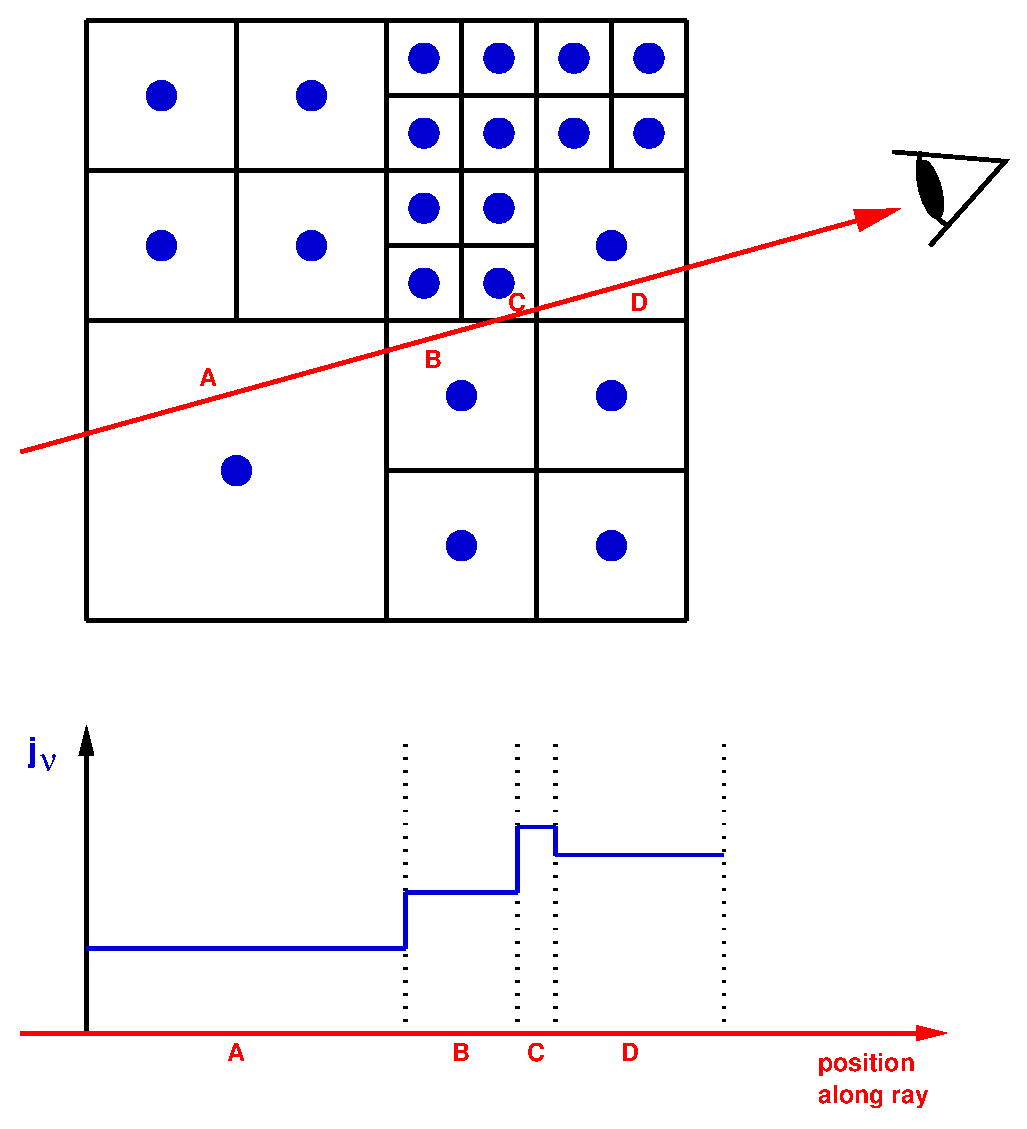
\includegraphics[width=0.45\textwidth]{cellcenter.eps}
  \hspace{3em}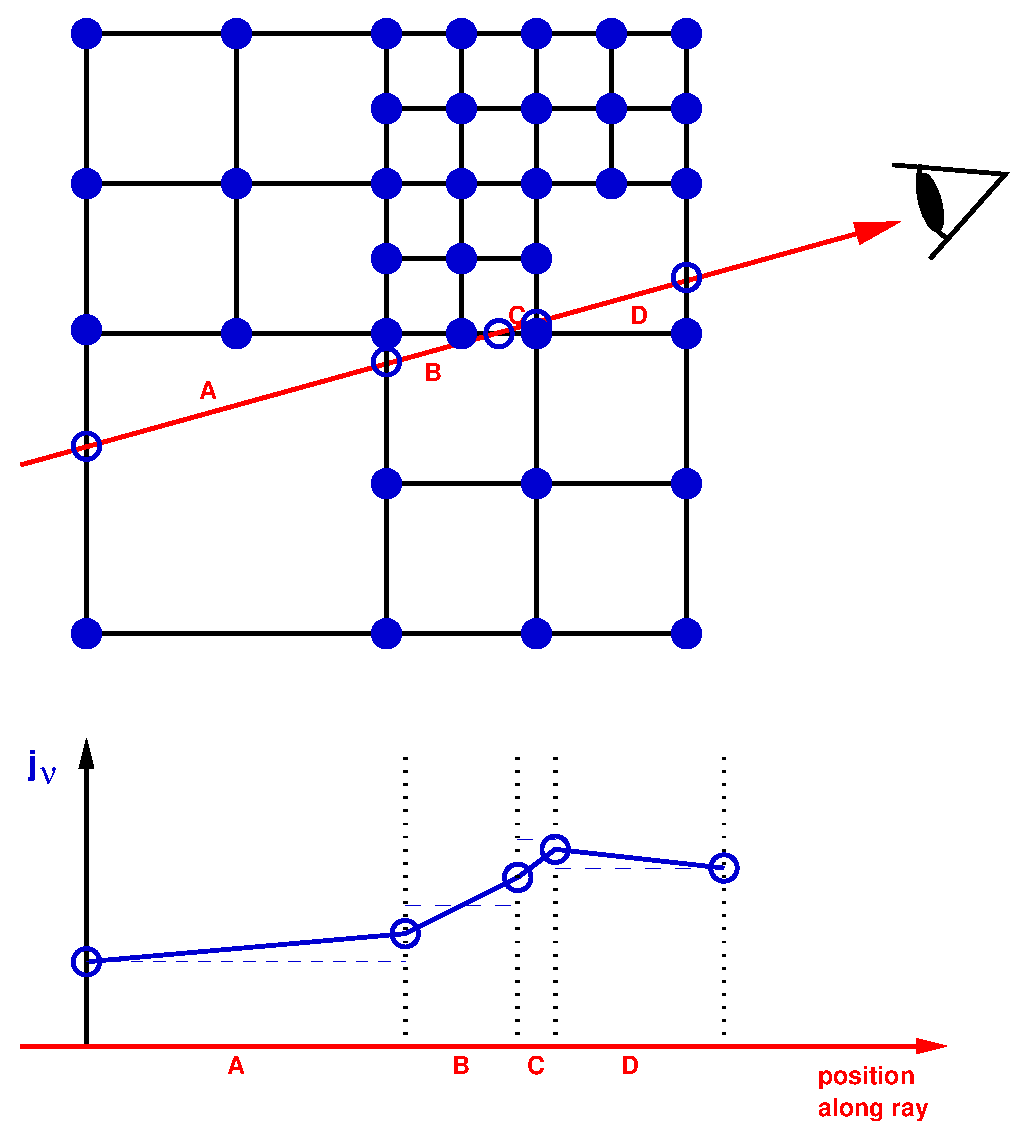
\includegraphics[width=0.45\textwidth]{cellcorner.eps}}
\caption{\label{fig-cellcenter-cellcorner}
%
  Pictographic representation of the integration of the transfer equation
  along a ray (red line with arrow head) through an AMR grid (black lines).
  The grid cuts the ray into ray segments A, B, C and D. At the bottom
  it is shown how the integrands are assumed to
  be along these four segments. Left: When using
  first order integration. The emissivity function $j_\nu$ and extinction
  function $\alpha_\nu$ are constant within each cell and thus constant
  along each
  ray segment. Right: When using second order integration. The emissivity 
  function $j_\nu$ and extinction
  function $\alpha_\nu$ are given at the cell corners (solid blue circles),
  and linearly interpolated from the cell corners
  to the locations where the ray crosses the cell walls (open blue circles).
  Then, along each ray segment the emissivity and extinction functions
  are assumed to be linear functions, so that the integration result is
  quadratic. The thin blue horizontal dashed lines are the same as those
  in the Left panel, and are just there for comparison. Note that these
  figures are 2-D, whereas this actually happens in 3-D. See Section
  \ref{sec-second-order} for more information.
%
}
\end{figure}
%
Ideally we would like to assure that the model grid is sufficiently finely
spaced everywhere. But in many cases of interest one does not have this
luxury. One must live with the fact that, for memory and/or computing time
reasons, the grid is perhaps a bit coarser than would be ideal. In such a
case it becomes important to consider the ``order'' of integration of the
transfer equation. By default, for images and spectra, RADMC-3D uses first
order integration: The source term and the opacity in each cell are assumed
to be constant over the cell. This is illustrated in
Fig.~\ref{fig-cellcenter-cellcorner}-Left. The integration over each cell
proceeds according to the following formula:
\begin{equation}
I_{\mathrm{result}} = I_{\mathrm{start}}e^{-\tau} + (1-e^{-\tau})S
\end{equation}
where $S=j/\alpha$ is the source function, assumed constant throughout the
cell, $\tau=\alpha\,\Delta s$ is the optical depth along the path that the
ray makes through the cell, and $I_{\mathrm{start}}$ is the intensity upon
entering the cell. This is the default used by RADMC-3D because the Monte
Carlo methods also treat cells as having constant properties over each
cell. This type of simple integration is therefore the closest to how the
Monte Carlo methods (thermal MC, scattering MC and mono MC) ``see'' the
grid. However, with first order integration the images look somewhat
``blocky'': you can literally see the block structure of the grid cells in
the image, especially if you make images at angles aligned with the
grid. For objects with high optical depths you may even see grid patterns in
the images.

RADMC-3D can also use second order integration for its images and spectra.
This is illustrated in Fig.~\ref{fig-cellcenter-cellcorner}-Right.
This is done with a simple ``{\small\tt secondorder}'' option added on the
command line, for instance:
\begin{asciibox}\begin{verbatim}
radmc3d image lambda 10 secondorder
\end{verbatim}\end{asciibox}
The integration now follows the formula (Olson et al.\ 1986):
\begin{equation}
I_{\mathrm{result}} = I_{\mathrm{start}}e^{-\tau} + (1-e^{-\tau}-\beta) S_{\mathrm{start}}
+ \beta S_{\mathrm{end}}
\end{equation}
with
\begin{equation}
\beta = \frac{\tau-1+e^{-\tau}}{\tau}
\end{equation}
and
\begin{equation}
\tau = \frac{\alpha_{\mathrm{start}}+\alpha_{\mathrm{end}}}{2}\Delta s
\end{equation}
For $\tau\rightarrow 0$ we have the limit $\beta\rightarrow \tau/2$, while
for $\tau\rightarrow \infty$ we have the limit $\beta\rightarrow 1$. 

The values of $\alpha$, $S$ etc., at the ``start'' position are obtained at
the cell interface where the ray enters the cell. The values at the ``end''
position are obtained at the cell interface where the ray leaves the cell.
The above formulas represent the exact solution of the transfer equation
along this ray-section if we assume that all variables are linear functions
between the ``start'' and ``end'' positions. 

The next question is: How do we determine the physical variables at the
cell interfaces (``start'' and ``end'')? After all, initially all variables
are stored for each cell, not for each cell interface or cell corner. The
way that RADMC-3D does this is:
\begin{itemize}
\item First create a ``grid of cell corners'', which we call the {\em vertex
    grid} (see the solid blue dots in
  Fig.~\ref{fig-cellcenter-cellcorner}-Right). The cell grid already
  implicitly defines the locations of all the cell corners, but these
  corners are, by default, not explicitly listed in computer memory. When
  the {\small\tt secondorder} option is given, however, RADMC-3D will
  explicitly find all cell corners and assign an identity (a unique integer
  number) to each one of them. NOTE: Setting up this vertex grid costs
  computer memory!
\item At each vertex (cell corner) the physical variables of the (up to) 8
  cells touching the vertex are averaged with equal weight for each cell.
  This now maps the physical variables from the cells to the vertices.
\item Whenever a ray passes through a cell wall, the physical variables of
  the 4 vertices of the cell wall are interpolated bilinearly onto the point
  where the ray passes through the cell wall (see the open blue circles in
  Fig.~\ref{fig-cellcenter-cellcorner}-Right). This gives the values at the
  ``start'' or ``end'' points. 
\item Since the current ``end'' point will be the ``start'' point for the
  next ray segment, the physical variables need only be obtained once per
  cell wall, as they can be recycled for the next ray segment. Each set of
  physical variables will thus be used twice: once for the ``end'' and once
  for the ``start'' of a ray segment (except of course at the very beginning
  and very end of the ray). 
\end{itemize}

%
\begin{figure}
\centerline{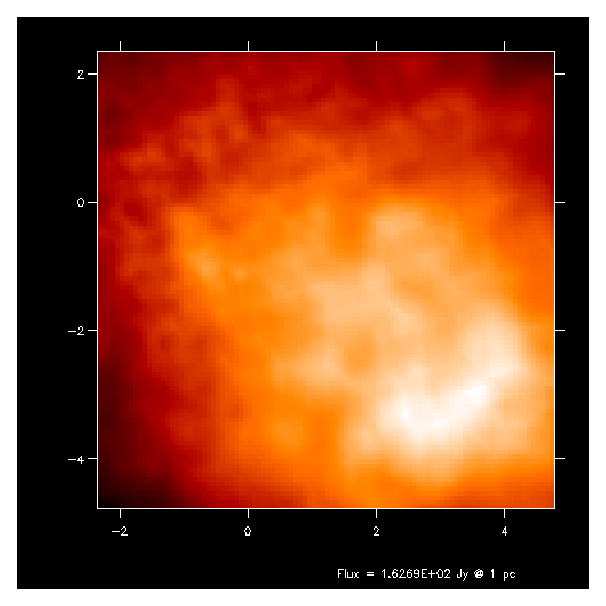
\includegraphics[width=0.3\textwidth]{simple_60_1st.eps}
            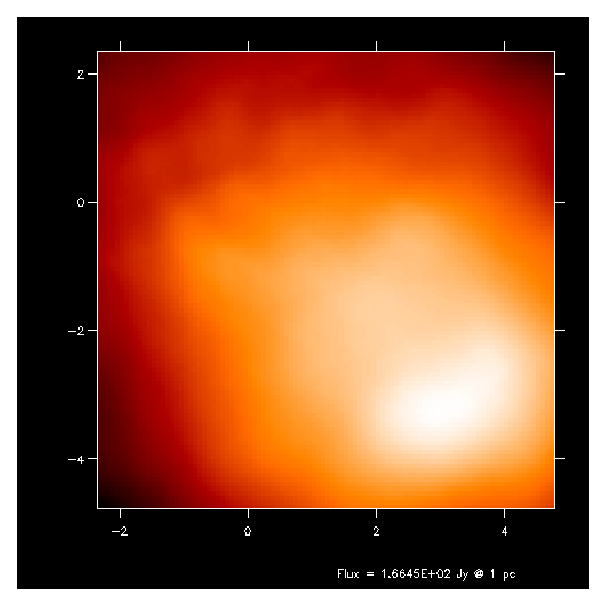
\includegraphics[width=0.3\textwidth]{simple_60_2nd.eps}}
\centerline{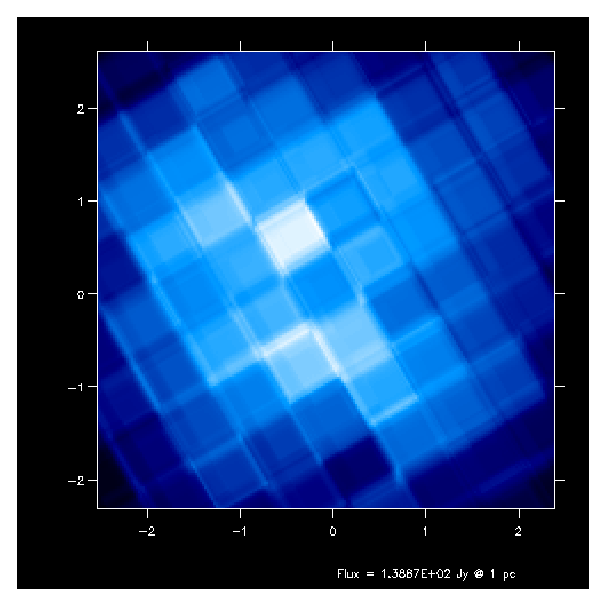
\includegraphics[width=0.3\textwidth]{simple_4_1st.eps}
            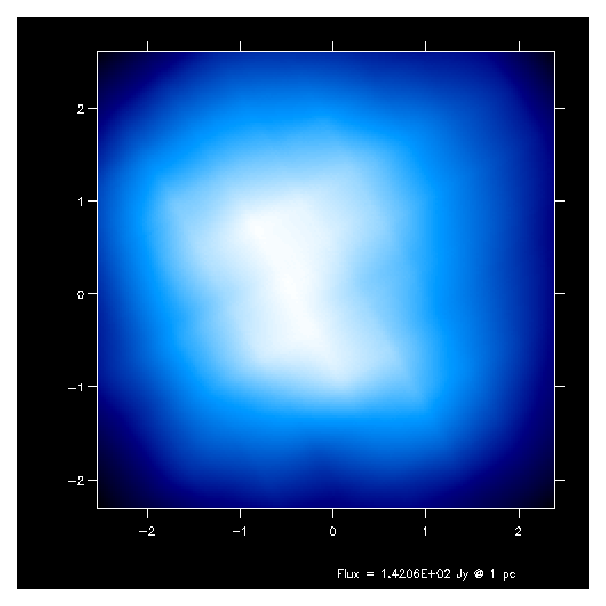
\includegraphics[width=0.3\textwidth]{simple_4_2nd.eps}}
\caption{\label{fig-effect-of-second-order-integration}
First-order integration of transfer equation in ray-tracing (left two
panels), versus second order integration (right two panels). Upper:
60 degrees inclination, Lower: 4 degrees inclination. Shown here is
the {\small\tt run\_simple\_1\_layers} model (in the {\small\tt examples}
directory) at $\lambda=10\;\mu$m at some zoom factor. See Section
  \ref{sec-second-order} for more information.
}
\end{figure}
%
If you compare the images or spectra obtained with first order integration
(default) or second order integration
(Fig.~\ref{fig-effect-of-second-order-integration}) you see that with the
first order method you still see the cell structure of the grid very much.
Also numerical noise in the temperature due to the Monte Carlo statistics
is much more prominent in the first order method. The second order method
makes much smoother results. 

For line transfer the second order mode can be even improved with the
``doppler catching method'', see Section \ref{sec-doppler-catching}.

{\bf WARNING:} Second order integration for the images and spectra from dust
continuum emission can in some cases lead to overestimation of the fluxes.
This is because the dust temperature calculated using the thermal Monte
Carlo algorithm assumes the temperature to be constant over each cell. The
second order integration for the images and spectra will, however, smear the
sources a bit out. This then leads to ``leaking'' of emissivity from
optically thick cells into optically thin cells. These optically thin cells
can then become too bright.

\subsection{Second order integration in spherical coordinates: a subtle issue}
\label{sec-secord-spher}
%
The second order integration (as well as the doppler-catching method, see
Section \ref{sec-doppler-catching}) work in cartesian coordinates as well as
in spherical coordinates. In spherical coordinates in 1-D (spherical
symmetry) or 2-D (axial symmetry) there is, however, a very subtle issue
that can lead to inaccuracies, in particular with line transfer. The problem
arises in the cell where a ray reaches its closest approach to the origin of
the coordinate system (or closest approach to the symmetry axis). There the
ray segment can become fairly long, and its angle with respect to the
symmetry axis and/or the origin can drastically change within this single
ray-segment. This can sometimes lead to inaccuracies. 

As of version 0.41 of {\small\tt RADMC-3D} a new global variable is
introduced, {\small\tt camera\_maxdphi}, which has as default the value 0.1,
but which can be set to another value in the {\small\tt radmc3d.inp} file.
It sets the maximum angle (in radian) which a ray segment in spherical
coordinates is allowed to span with respect to the origin of the coordinate
system. If a ray segment spans an angle larger than that, the ray-segment 
is cut into smaller segments. This means that in that cell the ray will
consist of more than one segment. 

If {\small\tt camera\_maxdphi=0} this segment cutting is switched off (for
backward compatibility to earlier versions of {\small\tt RADMC-3d}). 


\section{Visualizing the $\tau=1$ surface}
\label{sec-tausurf}
%
To be able to interpret the outcome of the radiative transfer calculations
it is often useful to find the spatial location of the $\tau=1$ surface (or,
for that matter, the $\tau=0.1$ surface or any $\tau=\tau_s$ surface) as
seen from the vantage point of the observer. This makes it easier to
understand where the emission comes from that you are seeing. RADMC-3D makes
this possible. Thanks to Peter Schilke and his team, for suggesting this
useful option.

The idea is to simply replace the command-line keyword {\small\tt image}
with  {\small\tt tausurf 1.0}. The $1.0$ stands for $\tau_s=1.0$, meaning
we will find the $\tau=1.0$ surface. Example: Normally you might make an
image with e.g.\ the following command:
\begin{asciibox}\begin{verbatim}
radmc3d image lambda 10 incl 45 phi 30
\end{verbatim}\end{asciibox}
Now you make a $\tau=1$ surface with the command:
\begin{asciibox}\begin{verbatim}
radmc3d tausurf 1.0 lambda 10 incl 45 phi 30
\end{verbatim}\end{asciibox}
or a $\tau=0.2$ surface with
\begin{asciibox}\begin{verbatim}
radmc3d tausurf 0.2 lambda 10 incl 45 phi 30
\end{verbatim}\end{asciibox}

The image output file {\small\tt image.out} will now contain, for each
pixel, the position along the ray in centimeters where $\tau=\tau_s$. The
zero point is the surface perpendicular to the direction of observation,
going through the pointing position (which is, by default $(0,0,0)$, but see
the description of {\small\tt pointau} in Section
\ref{sec-images}). Positive values mean that the surface is closer to the
observer than the plane, while negative values mean that the surface is
behind the plane.

If, for some pixel, there exists no $\tau=\tau_s$ point because the total
optical depth of the object for the ray belonging to that pixel is less
than $\tau_s$, then the value will be -1D91. 

You can also get the 3-D (i.e.~$x$, $y$, $z$) positions of each of these
points on the $\tau=\tau_s$ surface. They are stored in the file
{\small\tt tausurface\_3d.out}. There is a special IDL routine in the
{\small\tt readradmc.pro} file called {\small\tt read\_tausurf\_3d()}.
Also here the values of $x$, $y$, $z$ will be -1D91 for rays that
have total optical depth small than $\tau_s$.

If you do not use IDL for data handling, you can at least see the format
of the {\small\tt tausurface\_3d.out} file there. For most purposes, 
however, the projected data in the {\small\tt image.out} file should
be enough, however.

Note that if you make multi-frequency images, you will also get
multi-frequency $\tau=\tau_s$ surfaces. This can be particularly useful if
you want to understand the sometimes complex origins of the shapes of
molecular/atomic lines.

You can also use this option in the local observer mode, though I am not
sure how useful it is. Note, however, that in that mode the value stored in
the {\small\tt image.out} file will describe the distance in centimeter to
the local observer. The larger the value, the farther away from the observer
(contrary to the case of observer-at-infinity).

Example usage:
\begin{asciibox}\begin{verbatim}
radmc3d tausurf 1 lambda 10 incl 45 phi 30
idl
.r readradmc
a=readimage()
surface,a.image>(-1d15)
\end{verbatim}\end{asciibox}
This should, if your model is optically thick, show the $\tau=\tau_s$
surface. The {\small\tt >(-1d15)} in the last line is an IDL trick to
truncate the values of a.image to larger or equal to -1d15 centimeters
(which is a few AU). This is necessary because for all rays where the
total optical depth is less than $\tau_s$ (in this case 1) the value
would be -1D91.


\section{Using circularly arranged pixels for spectra (special topic)}
\label{sec-circular-pixel-arrangement}
%
{\bf For the moment, this mode is not yet finished}
%
% In the predecessor code (RADMC) the issue with flux conservation was dealt
% with using a trick different from subpixeling: Rather than arranging the
% pixels of the images in rows and columns, the pixels were arranged in
% concentric circles. The radii of these circles are tuned to the radii
% of the spherical coordinate system. In this way the huge dynamic range of
% scales of the model could be dealt with automatically.
% 
% Here, in RADMC-3D, we do not really need this trick, because of the new
% technique of recursive subpixeling (see Section
% \ref{sec-recursive-subpixeling}). 
% 
% But it might sometimes nevertheless be useful to use this circular pixel
% arrangement, because it is faster (though less reliable) than the recursive
% subpixeling. Also, the results would be easier to compare to the results of
% RADMC. But this mode works only when you use spherical coordinates! Also,
% there is no recursive subpixeling done when you use this mode, so if you use
% spherical coordinate {\em and} AMR grid refinement, then the refined regions
% may be not well resolved and flux may not be well conserved. And it works
% only for spectra. Images will remain rectangular pixel arrangements.
% 
% You can active it by the command-line option {\small\tt circ}, {\em iff} 
% you specified {\small\tt spectrum} or {\small\tt sed} as well.


\section{For public outreach work: local observers inside the model}
\label{sec-local-observer}
%
While it may not be very useful for scientific purposes (though there may be
exceptions), it is very nice for public outreach to be able to view a model
from the inside, as if you, as the observer, were standing right in the
middle of the model cloud or object. One can then use physical or
semi-physical or even completely ad-hoc opacities to create the right
'visual effects'. RADMC-3D has a viewing mode for this purpose. You can use
different projections:
\begin{itemize}
\item {\em Projection onto flat screen:}\\
  The simplest one is a projection onto a screen in front (or behind) the
  point-location of the observer. This gives an image that is good for
  viewing in a normal screen. This is the default ({\small\tt
    camera\_localobs\_projection=1}).
\item Another projection is a projection onto a sphere, which allow fields
  of view that are equal or larger than $2\pi$ of the sky. It may be useful
  for projection onto an OMNIMAX dome. This is projection mode {\small\tt
    camera\_localobs\_projection=2}.
\end{itemize}
You can set the variable {\small\tt camera\_localobs\_projection} to 1 or
2 by adding on the command line {\small\tt projection 2} (or 1), or by
setting it in the {\small\tt radmc3d.inp} as a line 
{\small\tt camera\_localobs\_projection = 2} (or 1). 

To use the local projection mode you must specify the following variables
on the command line:
\begin{itemize}
\item {\small\tt sizeradian}:\\
  This sets the size of the image in radian (i.e.\ the entire width of the
  image). Setting this will make the image width and height the same (like
  setting {\small\tt sizeau} in the observer-at-infinity mode, see Section
  \ref{sec-images}).
\item {\small\tt zoomradian}:\\
  {\em Instead} of {\small\tt sizeradian} you can also specify {\small\tt
    zoomradian}, which is the local-observer version of {\small\tt zoomau}
  or{\small\tt zoompc} (see Section \ref{sec-images}).
\item {\small\tt posang}:\\
  The position angle of the camera. Has the same meaning as in the
  observer-at-infinity mode.
\item {\small\tt locobsau} or {\small\tt locobspc}:\\
  Specify the 3-D location of the local observer inside the model in units
  of AU or parsec. This requires 3 numbers which are the x, y and z
  positions (also when using spherical coordinates for the model setup:
  these are still the cartesian coordinates).
\item {\small\tt pointau} or {\small\tt pointpc}:\\
  These have the same meaning as in the observer-at-infinity model.  They
  specify the 3-D location of the point of focus for the camera (to which
  point in space is the camera pointing) in units of AU or parsec. This
  requires 3 numbers which are the x, y and z positions (also when using
  spherical coordinates for the model setup: these are still the cartesian
  coordinates).
\item {\small\tt zenith} (optional):\\
  For Planetarium Dome projection ({\small\tt
    camera\_localobs\_projection=2}) it is useful to make the pointing
  direction not at the zenith (because then the audience will always have to
  look straight up) but at, say, 45 degrees. You can facilitate this
  (optionally) by adding the command line option {\small\tt zenith 45} for a
  45 degrees offset. This means that if you are sitting under the OMNIMAX
  dome, then the camera pointing (see {\small\tt pointau} above) is 45
  degrees in front of you rather than at the zenith. This option is highly
  recommended for dome projections, but you may need to play with the angle
  to see which gives the best effect.
\end{itemize}
Setting {\small\tt sizeradian}, {\small\tt zoomradian}, {\small\tt locobsau}
or {\small\tt locobspc} on the command line automatically switches to the
local observer mode (i.e.\ there is no need for an extra keyword setting the
local observer mode on). To switch back to observer-at-infinity mode, you
specify e.g.~{\small\tt incl} or {\small\tt phi} (the direction toward which
the observer is located in the observer-at-infinity mode). Note that if you
accidently specify both e.g.~{\small\tt sizeradian} and {\small\tt incl},
you might end up with the wrong mode, because the mode is set by the last
relevant entry on the command line.

The images that are produced using the local observer mode will have the x-
and y- pixel size specifications in radian instead of cm. The first line of
an image (the format number of the file) contains then the value 2
(indicating local observer image with pixel sizes in radian) instead of 1
(which indicates observer-at-infinity image with pixel sizes in cm).

{\em NOTE: For technical reasons dust scattering is (at least for now) not
included in the local observer mode! It is discouraged to use the local
observer mode for scientific purposes.}



\section{Multiple vantage points: the ``Movie'' mode}
\label{sec-movie-mode}
%
It can be useful, both scientifically and for public outreach, to make
movies of your model, for instance by showing your model from different
vantage points or by ``travelling'' through the model using the local
observer mode (Section \ref{sec-local-observer}). For a movie one must
make many frames, each frame being an image created by RADMC-3D's image
capabilities. If you call {\small\tt radmc3d} separately for each
image, then often the reading of all the large input files takes up
most of the time. One way to solve this is to call {\small\tt radmc3d}
in ``child mode'' (see Chapter \ref{chap-child-mode}). But this is 
somewhat complicated and cumbersome. A better way is to use RADMC-3D's
``movie mode''. This allows you to ask RADMC-3D to make a sequence of
images in a single call. The way to do this is to call {\small\tt radmc3d}
with the {\small\tt movie} keyword:
{\small\begin{verbatim}
radmc3d movie
\end{verbatim}}
This will make {\small\tt radmc3d} to look for a file called 
{\small\tt movie.inp} which contains the information about each image
it should make. The structure of the {\small\tt movie.inp} file is:
\begin{asciibox}\begin{verbatim}
iformat
nframes
<<information for frame 1>>
<<information for frame 2>>
<<information for frame 3>>
...
<<information for frame nframes>>
\end{verbatim}\end{asciibox}
The {\small\tt iformat} is an integer that is described below.  The
{\small\tt nframes} is the number of frames. The {\small\tt $<<$information
  for frame xx$>>$} are lines containing the information of how the camera
should be positioned for each frame of the movie (i.e.\ for each imag). It
is also described below.

There are multiple ways to tell RADMC-3D how to make
this sequence of images. Which if these ways RADMC-3D should use is specified
by the {\small\tt iformat} number. Currently there are 2, but later we may add
further possibilities. Here are the current possibilities
\begin{itemize}
\item {\bf iformat=1:}\\
The observer is at infinity (as usual) and the {\small\tt $<<$information
  for frame xx$>>$} consists of the following numbers (separated by
spaces):
\begin{asciibox}\begin{verbatim}
pntx pnty pntz hsx hsy pa incl phi
\end{verbatim}\end{asciibox}
These 8 numbers have the following meaning:
\begin{itemize}
\item {\small\tt pntx,pnty,pntz}\\
  These are the x, y and z coordinates (in units of cm) of the point toward
  which the camera is pointing.
\item {\small\tt hsx,hsy}\\
  These are the image half-size in horizontal and vertical direction on the
  image (in units of cm). 
\item {\small\tt pa}\\
  This is the position angle of the camera in degrees.
  This has the same meaning as for a single image.
\item {\small\tt incl,phi}\\
  These are the inclination and phi angle toward the observer in degrees.
  These have the same meaning as for a single image.
\end{itemize}
\item {\bf iformat=-1:}\\
 The observer is local (see Section
  \ref{sec-local-observer}) and the {\small\tt $<<$information for frame
    xx$>>$} consists of the following numbers (separated by spaces):
\begin{asciibox}\begin{verbatim}
pntx pnty pntz hsx hsy pa obsx obsy obsz
\end{verbatim}\end{asciibox}
These 9 numbers have the following meaning:
\begin{itemize}
\item {\small\tt pntx,pnty,pntz,hsx,hsy,pa}\\
  Same meaning as for iformat=1.
\item {\small\tt obsx,obsy,obsz}\\
  These are the x, y and z position of the local observer (in units of cm).
\end{itemize}
\end{itemize}
Apart from the quantities that are thus set for each image separately, 
all other command-line options still remain valid. 

Example, let us make a movie of 360 frames of a model seen at infinity while
rotating the object 360 degrees, and as seen at a wavelength of
$\lambda=10\mu$m with 200x200 pixels. We construct the {\small\tt movie.inp}
file:
\begin{asciibox}\begin{verbatim}
1
360
0. 0. 0. 1d15 1d15 0. 60.  1.
0. 0. 0. 1d15 1d15 0. 60.  2.
0. 0. 0. 1d15 1d15 0. 60.  3.
.
.
.
0. 0. 0. 1d15 1d15 0. 60.  358.
0. 0. 0. 1d15 1d15 0. 60.  359.
0. 0. 0. 1d15 1d15 0. 60.  360.
\end{verbatim}\end{asciibox}
We now call RADMC-3D in the following way:
{\small\begin{verbatim}
radmc3d movie lambda 10. npix 200
\end{verbatim}}
This will create image files {\small\tt image\_0001.out}, 
{\small\tt image\_0002.out},
all the way to {\small\tt image\_0360.out}.
The images will have a full width and height of $2\times 10^{15}$cm (about
130 AU), will always point to the center of the image, will be taken at an
inclination of 60 degrees and with varying $\phi$-angle.

Another example: let us move through the object (local observer mode),
approaching the center very closely, but not precisely:
\begin{asciibox}\begin{verbatim}
-1
101
0. 0. 0. 0.8 0.8 0. 6.d13 -1.0000d15 0.
0. 0. 0. 0.8 0.8 0. 6.d13 -0.9800d15 0.
0. 0. 0. 0.8 0.8 0. 6.d13 -0.9600d15 0.
.
.
0. 0. 0. 0.8 0.8 0. 6.d13 -0.0200d15 0.
0. 0. 0. 0.8 0.8 0. 6.d13  0.0000d15 0.
0. 0. 0. 0.8 0.8 0. 6.d13  0.0200d15 0.
.
.
0. 0. 0. 0.8 0.8 0. 6.d13  0.9600d15 0.
0. 0. 0. 0.8 0.8 0. 6.d13  0.9800d15 0.
0. 0. 0. 0.8 0.8 0. 6.d13  1.0000d15 0.
\end{verbatim}\end{asciibox}
Here the camera automatically rotates such that the focus remains on the
center, as the camera flies by the center of the object at a
closest-approach to the center of $6\times 10^{13}$cm. The half-width
of the image is 0.8 radian.

{\em Important note:} If you have scattering switched on, then every
rendering of an image makes a new scattering Monte Carlo run. Since Monte
Carlo produces noise, this would lead to a movie that is very jittery
(every frame has a new noise set). It is of course best to avoid this
by using so many photon packages that this is not a concern. But in 
practice this may be very CPU-time consuming. You can also fix the noise
in the following way: add {\small\tt resetseed} to the command-line call:
{\small\begin{verbatim}
radmc3d movie resetseed
\end{verbatim}}
and it will force each new scattering Monte Carlo computation to start
with the same seed, so that the photons will exactly move along the same
trajectories. Now only the scattering phase function will change because
of the different vantage points, but not the Monte Carlo noise. You can 
in fact set the actual value of the initial seed in the {\small\tt
radmc3d.inp} file by adding a line 
{\small\begin{verbatim}
iseed = -5415
\end{verbatim}}
(where -5415 is to be replaced by the value you want) to the {\small\tt
  radmc3d.inp} file. Note also that if your
movie goes through different wavelengths, the resetseed will likely not help
fixing the noisiness, because the paths of photons will change for different
wavelengths, even with the same initial seed.

% \section{For developers: some details on the internal workings}
% {\em [This section is only interesting for developers]}
% 
% \subsection{Multi-wavelength images and spectra: two methods (1 and 2)}
% \label{subsec-multiwavelength-methods}
% 
% {\bf [TO BE COMPLETED]}
% 
% 
% \subsection{Ray-tracing: two methods (A and B)}
% \label{subsec-raytrace-methods}
% The camera module of RADMC-3D features two different ways of tracing
% a ray for making images and spectra:
% \begin{itemize}
% \item{} {\bf Method A:} Tracing in a sequential step-by-step fashion,
%   whereby at each step the opacities are computed, the intensities are
%   updated and the next position of the ray in the 3-D model is determined.
%   This is the method by default, and it the simplest method. But it may
%   not always be the most optimized in terms of speed.
% \item{} {\bf Method B:} First find out how the ray goes through the 3-D
%   model, and prepare a 1-D array of dust tempetures and densities, line
%   transfer quantities (such as level populations etc) and $\Delta s$ values
%   (length of ray elements). Then compute the opacities at each point.  Then
%   finally do the 1-D formal transfer. This method has the advantage that it
%   lends itself well for parallellization on a GPU (which only gives speed-up
%   if method 2 is used for multi-wavelength images and spectra, see Section
%   \ref{subsec-multiwavelength-methods}). Also, by scouting the entire ray
%   before doing the full transfer -- the automatic line/level subsubset
%   selection for the line transfer (see Section
% ###############################
% ###############################
% ###############################
% ###############################
%   \ref{subsec-automatic-subsubset}) -- can be done and may give some speed
%   up in some cases for the line ray-tracing.
% \end{itemize}


%----------------------------------------------------------------------------
%                      CHAPTER: MORE ABOUT GRIDS
%----------------------------------------------------------------------------
\chapter{More information about the gridding}
\label{chap-gridding}
%
We already discussed the various types of grids in Section
\ref{sec-spatial-grid}, and the grid input file structure is described in
Section \ref{sec-grid-input}. In this chapter let us take a closer look
at the gridding possibilities and things to take special care of.


\section{Regular grids}
\label{sec-regular-grid}
A regular grid is called ``grid style 0'' in RADMC-3D. It can be used in
Cartesian coordinates as well as in spherical coordinates (Section
\ref{sec-coord-systems}).

A regular grid, in our definition, is a multi-dimensional grid which is
separable in $x$, $y$ and $z$ (or in spherical coordinates in $r$, $\theta$
and $\phi$). You specify a 1-D monotonically increasing array of values
$x_1, x_2,\cdots,x_{\mathrm{nx+1}}$ which represent the cell walls in
$x-direction$.  You do the same for the other directions: $y_1,
y_2,\cdots,y_{\mathrm{ny+1}}$ and $z_1, z_2,\cdots,z_{\mathrm{nz+1}}$.  The
value of, say, $x_2$ is the same for every position in $y$ and $z$: this is
what we mean with ``separable''.

In Cartesian coordinates RADMC-3D enforces perfectly cubic grid cells (i.e.\
linear grids). But that is only to make the image sub-pixeling easier (see
Section \ref{sec-recursive-subpixeling}). For spherical grids this is not
enforced, and in fact it is strongly encouraged to use non-linear grids in
spherical coordinates. Please read Section \ref{sec-separable-refinement}
if you use spherical coordinates!

In a regular grid you specify the grids in each direction separately.  For
instance, the x-grid is given by specifying the cell walls in
x-direction. If we have, say, 10 cells in x-direction, we must specify 11
cell wall positions. For instance: $x_i=\{-5,-4,-3,-2,-1,0,1,2,3,4,5\}$.
For the $y$-direction and $z$-direction likewise. Fig.~\ref{fig-regular-grid}
shows an example of a 2-D regular grid of 4x3 cells.
%
\begin{figure}
\centerline{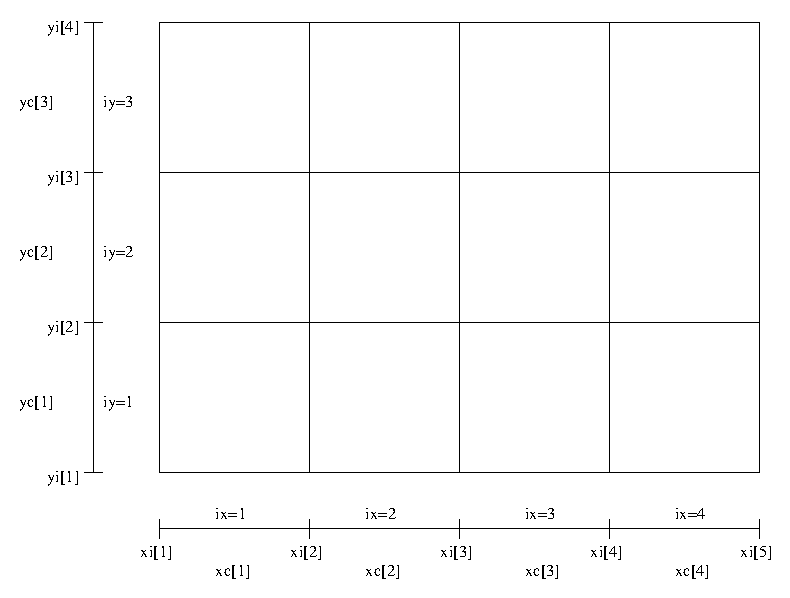
\includegraphics[width=0.6\textwidth]{base_amr_bare.eps}}
\caption{\label{fig-regular-grid}
Example of a regular 2-D grid with {\small\tt nx}=4 and {\small\tt ny}=3.
}
\end{figure}
%
In Cartesian coordinates we typically define our model in full 3-D.
However, if your problem has translational symmetries, you might also want
to consider the 1-D plane-parallel mode (see Section
\ref{sec-1d-plane-parallel}) or the 2-D pencil-parallel mode 
(see Section \ref{sec-2d-pencil-parallel}). 

In full 3-D Cartesian coordinates the cell sizes {\em must} be perfectly
cubical, i.e.\ the spacing in each direction must be the same. If you need a
finer grid in some location, you can use the AMR capabilities discussed
below.

In spherical coordinates you can choose between 1-D spherically symmetric
models, 2-D axisymmetric models or fully 3-D models. In spherical coordinates
you do {\em not} have restrictions to the cell geometry or grid spacing. 
You can choose any set of numbers $r_1,\cdots,r_{\mathrm{nr}}$ as radial
grid, as long as this set of numbers is larger than 0 and monotonically
increasing. The same is true for the $\theta$-grid and the $\phi$-grid.

The precise way how to set up a regular grid using the {\small\tt
  amr\_grid.inp} file is described in Section \ref{sec-amr-grid-regular}.
The input of any spatial variables (such as e.g.\ the dust density) uses the
sequence of grid cells in the same order as the cells are specified in that
{\small\tt amr\_grid.inp} file. 

For input and output data to file, for stuff on a regular grid, the order of
nested loops over coordinates would be:
\begin{asciibox}\begin{verbatim}
do iz=1,amr_grid_nz
   do iy=1,amr_grid_ny
      do ix=1,amr_grid_nx
         << read or write your data >>
      enddo
   enddo
enddo
\end{verbatim}\end{asciibox}

For spherical coordinates we have the following association: $x\rightarrow r$,
$y\rightarrow \theta$, $z\rightarrow \phi$.




\section{Separable grid refinement in spherical coordinates (important!)}
\label{sec-separable-refinement}
%
Spherical coordinates are a very powerful way of dealing with
centrally-concentrated problems. For instance, collapsing protostellar
cores, protoplanetary disks, disk galaxies, dust tori around active galactic
nuclei, accretion disks around compact objects, etc. In other words:
problems in which a single central body dominates the problem, and material
at all distances from the central body matters. For example a disk around
a young star goes all the way from 0.01 AU out to 1000 AU, covering 5
orders of magnitude in radius. Spherical coordinates are the easiest way 
of dealing with such a huge radial dynamic range: you simply make a radial
grid, where the grid spacing $r_{i+1}-r_i$ scales roughly with $r_i$. 

This is called a {\em logarithmic radial grid}. This is a grid whith a
spacing in which $(r_{i+1}-r_i)/r_i$ is constant with $r$. In this way you
assure that you have always the right spatial resolution in $r$ at each
radius. In spherical coordinates it is highly recomended to use such a log
spacing. But you can also refine the $r$ grid even more (in addition to the
log-spacing). This is also strongly recommended near the inner edge of a
circumstellar shell, for instance.  Or at the inner dust rim of a
disk. There you must refine the $r$ grid (by simply making the spacing
smaller as you approach the inner edge from the outside) to assure that the
first few cells are optically thin and that there is a gradual transition
from optically thin to optically thick as you go outward. This is
particularly important for, for instance, the inner rim of a dusty disk.

In spherical coordinates you can vary the spacing in $r$, $\theta$ and
$\phi$ completely freely. That means: you could have for instance $r$
to be spaced as $1.00, 1.01, 1.03, 1.05, 1.1, 1.2, 1.35, \cdots$. There is
no restriction, as long as the coordinate points are monotonically
increasing. In Figure \ref{fig-spher-sep-ref} this is illustrated. 

{\em Note that in addition to separable refinement, also AMR refinement
is possible in spherical coordinates. See Section \ref{sec-oct-tree-amr}.}

%
\begin{figure}
\centerline{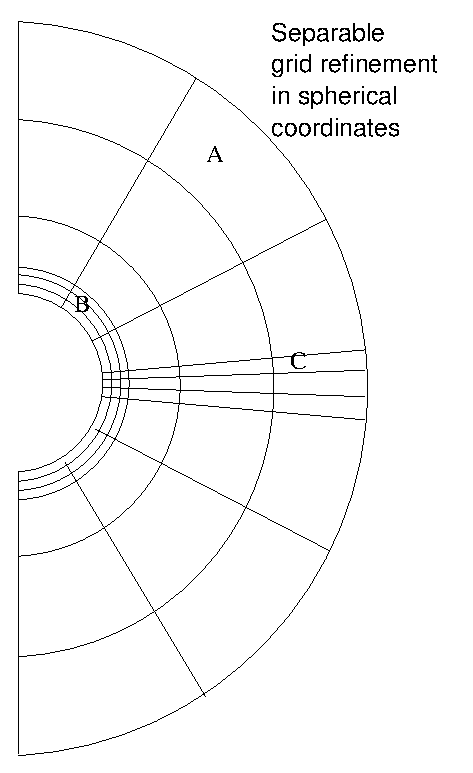
\includegraphics[width=0.28\textwidth]{spher_grid_ref_txt.eps}
\hspace{4em}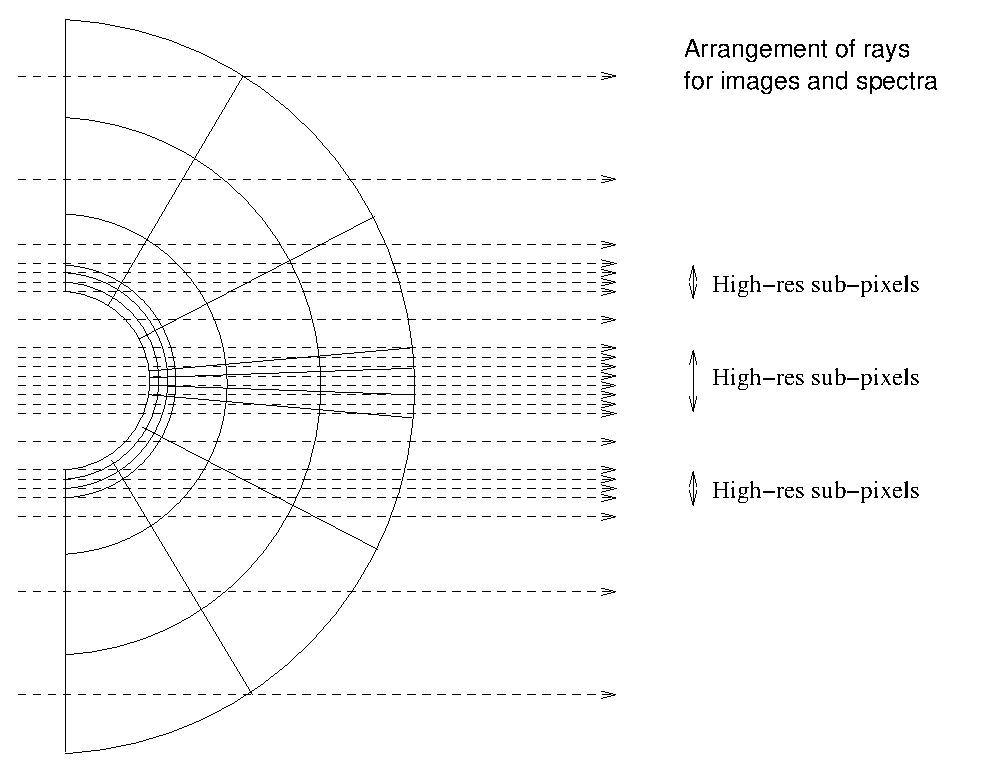
\includegraphics[width=0.6\textwidth]{spher_grid_ref_rays.eps}}
\caption{\label{fig-spher-sep-ref} Example of a spherical 2-D grid in which
  the radial and $\theta$ grids are refined in a ``separable'' way. In
  radial direction the inner cells are refined (``B'' in the right figure)
  and in $\theta$ direction the cells near the equatorial plane are refined
  (``C'' in the right figure). This kind of grid refinement does not require
  oct-tree AMR: the grid remains separable. For models in which the inner
  grid edge is also the inner model edge (e.g.\ a simple model of a
  protoplanetary disk with a sharp inner cut-off) this kind of separable
  grid refinement in $R$-direction may be essential to avoid problems with
  optically thick inner cells (see e.g.\ Fig.\ \ref{fig-innerrim-lowres} for
  an example of what could go wrong if you do not do this). Separable grid
  refinement in $\Theta$-direction is typically important for protoplanetary
  disk models, where the midplane and surface layers of the disk need to
  have sufficient resolution, but any possible surrounding spherical nebula
  may not. Left: When making an image, RADMC-3D will automatically make
  ``sub-pixels'' to ensure that all structure of the model as projected on
  the sky of the observer are spatially resolved.  Extreme grid refinement
  leads thus to extreme sub-pixeling. See Section
  \ref{sec-rec-subpixel-spher-coord} for details, and ways to prevent
  excessive sub-pixeling when this is not necessary.}
\end{figure}
%

For models of accretion disks it can, for instance, be useful to make sure
that there are more grid points of $\theta$ near the equatorial plane
$\theta=\pi/2$. So the grid spacing between $\theta=0.0$ and $\theta=1.0$
may be very coarse while between $\theta=1.0$ and $\theta=\pi/2$ you may
put a finer grid. All of this ``grid refinement'' can be done without
the ``AMR'' refinement technique: this is the ``separable'' grid refinement,
because you can do this separately for $r$, for $\theta$ and for $\phi$.

Sometimes, however, separable refinement may not help you to refine the grid
where necessary. For instance: if you model a disk with a planet in the
disk, then you may need to refine the grid around the planet. You could
refine the grid in principle in a separable way, but you would then have a
large redundancy in cells that are refined by far away from the planet.  Or
if you have a disk with an inner rim that is not exactly at
$r=r_{\mathrm{rim}}$, but is a rounded-off rim. In these cases you need
refinement exactly located at the region of interest. For that you need the
``AMR'' refinement (Sections \ref{sec-oct-tree-amr} and \ref{sec-layered-amr}).

{\em Important note:} When using strong refinement in one of the coordinates
$r$, $\theta$ or $\phi$, image-rendering and spectrum-rendering can become
very slow, because of the excessive sub-pixeling this causes. There are ways
to limit the sub-pixeling for those cases. See the Section on sub-pixeling
in spherical coordinate: Section \ref{sec-rec-subpixel-spher-coord}.


\section{Oct-tree Adaptive Mesh Refinement}
\label{sec-oct-tree-amr}
%
An oct-tree refinened grid is called ``grid style 1'' in RADMC-3D. It can be
used in Cartesian coordinates as well as in spherical coordinates (Section
\ref{sec-coord-systems}). 

You start from a normal regular base grid (see Section
\ref{sec-regular-grid}), possibly even with ``separable refinement'' (see
Section \ref{sec-separable-refinement}). You can then split some of the cells
into 2x2x2 subcells (or more precisely: in 1-D 2 subcells, in 2-D 2x2
subcells and in 3-D 2x2x2 subcells). If necessary, each of these 2x2x2
subcells can also be split into further subcells. This can be repeated as
many times as you wish until the desired grid refinement level is reached.
Each refinement step refines the grid by a factor of 2 in linear dimension,
which means in 3-D a factor of 8 in volume. In this way you get, for each
refined cell of the base grid, a tree of refinement. The base grid can have
any size, as long as the number of cells in each direction is an even
number. For instance, you can have a 6x4 base grid in 2-D, and refine cell
(1,2) by one level, so that this cell splits into 2x2 subcells.

Note that it is important to set which dimensions are ``active'' and which
are ``non-active''. For instance, if you have a 1-D model with 100 cells and
you tell RADMC-3D (see Section \ref{sec-amr-grid-oct-tree}) to make a base
grid of 100x1x1 cells, but you still keep all three dimensions ``active''
(see Section \ref{sec-amr-grid-oct-tree}), then a refinement of cell 1
(which is actually cell (1,1,1)) will split that cell into 2x2x2 subcells,
i.e.\ it will also refine in y and z direction. Only if you explicitly
switch the y and z dimensions off the AMR will split it into just 2
subcells.

Oct-tree mesh refinement is very powerful, because it allows you to refine
the grid exactly there where you need it. And because we start from a
regular base grid like the grid specified in Section \ref{sec-regular-grid},
we can start designing our model on a regular base grid, and then refine
where needed. See Fig.~\ref{fig-oct-tree-amr}
%
\begin{figure}
\centerline{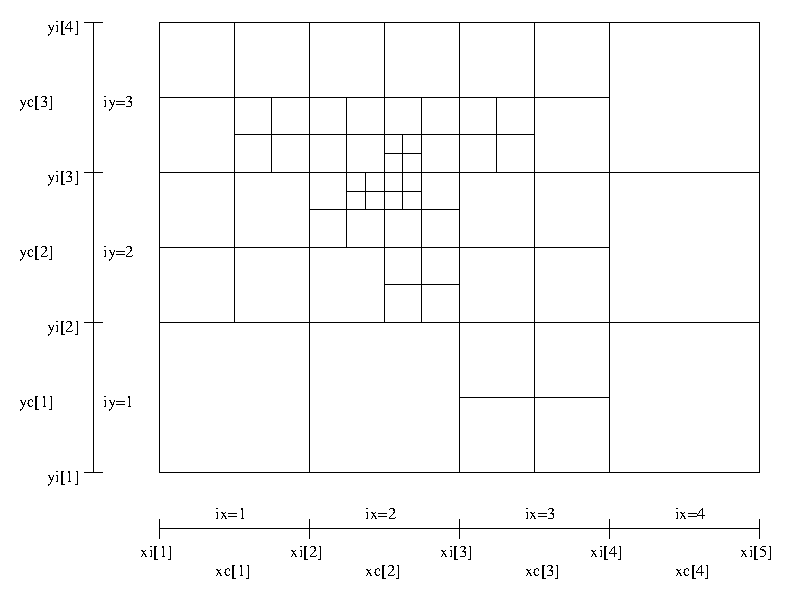
\includegraphics[width=0.6\textwidth]{oct_tree_amr_bare.eps}}
\caption{\label{fig-oct-tree-amr}
Example of a 2-D grid with oct-tree refinement. The base grid has
{\small\tt nx}=4 and {\small\tt ny}=3. Three levels of refinement are
added to this base grid. 
}
\end{figure}
%

The AMR stand for ``Adaptive Mesh Refinement'', which may suggest that 
RADMC-3D will refine internally. At the moment this is not yet the case.
The ``adaptive'' aspect is left to the user: he/she will have to ``adapt''
the grid such that it is sufficiently refinened where it is needed. In the
future we may allow on-the-fly adaption of the grid, but that is not yet
possible now. 

One problem with oct-tree AMR is that it is difficult to handle such grids
in external plotting programs, or even in programs that set up the grid.
While it is highly flexible, it is not very user-friendly. Typically you may
use this oct-tree refinement either because you import data from a
hydrodynamics code that works with oct-tree refinement (e.g.\ FLASH,
RAMSES), or when you internally refine the grid using the {\small\tt
  userdef\_module.f90} (see Chapter \ref{chap-internal-setup}). In the
former case you are anyway forced to manage the complexities of AMR, while
in the latter case you can make use of the AMR modules of RADMC-3D
internally to handle them. But if you do not need to full flexibility of
oct-tree refinement and want to use a simpler kind of refinement, then
you can use RADMC-3D's alternative refinement mode: the layer-style
AMR described in Section \ref{sec-layered-amr} below.

The precise way how to set up such an oct-tree grid using the {\small\tt
  amr\_grid.inp} file is described in Section \ref{sec-amr-grid-oct-tree}.
The input of any spatial variables (such as e.g.\ the dust density) uses the
sequence of grid cells in the same order as the cells are specified in that
{\small\tt amr\_grid.inp} file.


\section{Layered Adaptive Mesh Refinement}
\label{sec-layered-amr}
%
A layer-style refinened grid is called ``grid style 10'' in RADMC-3D. It can
be used in Cartesian coordinates as well as in spherical coordinates
(Section \ref{sec-coord-systems}).

This is an alternative to the full-fledged oct-tree refinement of Section
\ref{sec-oct-tree-amr}. The main advantage of the layer-style refinement is
that it is far easier to handle by the human brain, and thus easier for 
model setup  and the analysis of the results. 

The idea here is that you start again with a regular grid (like that of
Section \ref{sec-regular-grid}), but you can now specify a rectangular
region which you want to refine by a factor of 2. The way you do this is by
choosing the starting indices of the rectangle and specifying the size of
the rectangle by setting the number of cells in each direction from that
starting point onward. For instance, setting the starting point at (2,3,1)
and the size at (1,1,1) will simply refine just cell (2,3,1) of the base
grid into a set of 2x2x2 sub-cells. But setting the starting point at
(2,3,1) and the size at (2,2,2) will split cells (2,3,1), (3,3,1), (2,4,1),
(3,4,1), (2,3,2), (3,3,2), (2,4,2) and (3,4,2) each into 2x2x2 subcells.
This in fact is handled as a 4x4x4 regular sub-grid patch. And setting the
starting point at (2,3,1) and the size at (4,6,8) will make an entire
regular sub-grid patch of 8x12x16 cells. Such a sub-grid patch is
called a {\em layer}.

The nice thing of these layers is that each layer (i.e.\ subgrid patch) is
handled as a regular sub-grid. The base grid is layer number 0, and the
first layer is layer number 1, etc. Each layer (including the base grid) can
contain multiple sub-layers. The only restriction is that each layer fits
entirely inside its parent layer, and layers with the same parent layer
should not overlap. Each layer can thus have one or more sub-layers, each of
which can again be divided into sub-layers. This builds a tree structure,
with the base layer as the trunk of the tree (this is contrary to the
oct-tree structure, where each base grid {\em cell} forms the trunk of its
own tree). In Fig.~\ref{fig-twolayer-amr} an example is shown of two layers
with the same parent (= layer 0 = base grid), while in
Fig.~\ref{fig-nestedlayer-amr} an example is shown of two nested layers.
%
\begin{figure}
\centerline{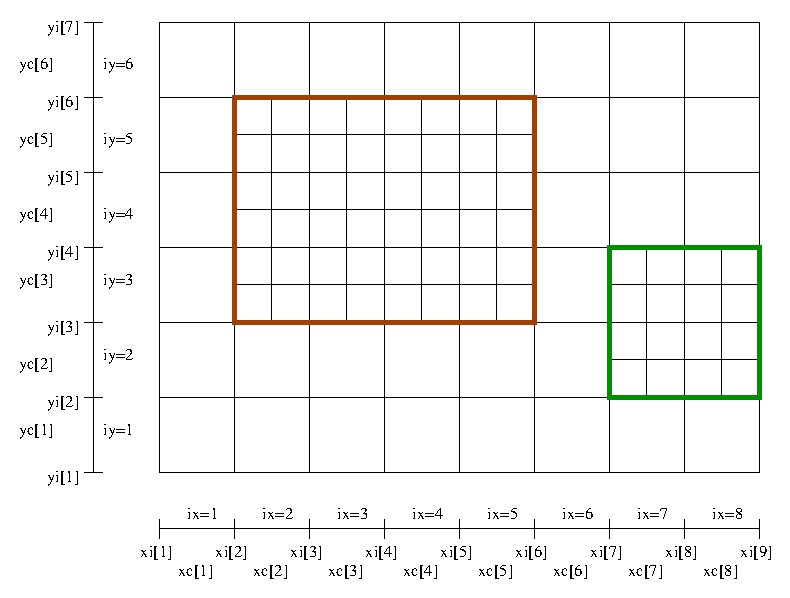
\includegraphics[width=0.6\textwidth]{twolayer_bare.eps}}
\caption{\label{fig-twolayer-amr} Example of a 2-D base grid with {\small\tt
    nx}=4 and {\small\tt ny}=3, with two AMR-layers added to it.  This
  example has just one level of refinement, as the two layers (brown and
  gree) are on the same level (they have the same parent layer = layer 0).
}
\end{figure}
%
\begin{figure}
\centerline{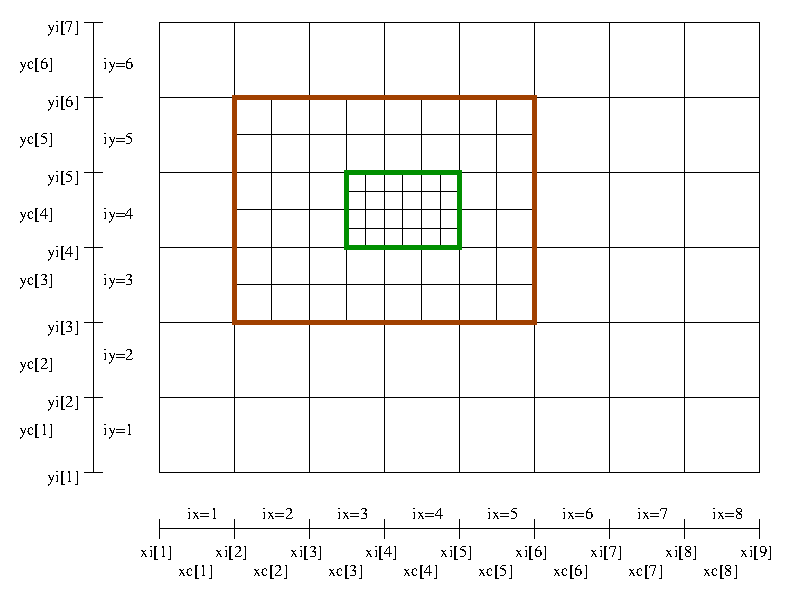
\includegraphics[width=0.6\textwidth]{nestedlayer_bare.eps}}
\caption{\label{fig-nestedlayer-amr} Example of a 2-D base grid with
  {\small\tt nx}=4 and {\small\tt ny}=3, with two nested AMR-layers added to
  it.  This example has two levels of refinement, as layer 1 (brown) is the
  parent of layer 2 (green).  }
\end{figure}
%


If you now want to specify data on this grid, then you simply specify it on
each layer separately, as if each layer is a separate entity. Each layer is
treated as a regular grid, irrespective of whether it contains sub-layers
or not. So if we have a base grid of 4x4x4 grid cells containing two layers:
one starting at (1,1,1) and having (2,2,2) size and another starting at
(3,3,3) and having (1,1,2) size, then we first specify the data on the 
4$^3$=64 base grid, then on the (2*2)$^3$=64 grid cells of the first
layer and then on the 2x2x4=16 cells of the second layer. Each of these
three layers are regular grids, and the data is inputted/outputted in
the same way as if these are normal regular grids (see Section
\ref{sec-regular-grid}). But instead of just one such regular grid, now
the data file (e.g.\ {\small\tt dust\_density.inp}) will contain three
successive lists of numbers, the first for the base grid, the second for
the first layer and the last for the second layer. You may realize at this
point that this will introduce a redundancy. See Subsection
\ref{sec-layer-amr-redundancy} for a discussion of this redundancy.

The precise way how to set up such an oct-tree grid using the {\small\tt
  amr\_grid.inp} file is described in Section \ref{sec-amr-grid-layered}.
The input of any spatial variables (such as e.g.\ the dust density) uses the
sequence of grid cells in the same order as the cells are specified in that
{\small\tt amr\_grid.inp} file. 

\subsection{On the ``successively regular'' kind of data storage, and its slight
  redundancy}
%
\label{sec-layer-amr-redundancy}
With the layered grid refinement style there will be {\em redundant} data in
the data files (such as e.g.\ the {\small\tt dust\_density.inp} file. Each
layer is a regular (sub-)grid and the data will be specified in each of
these grid cells of that regular (sub-)grid.  If then some of these cells
are overwritten by a higher-level layer, these data are then redundant. We
could of course have insistent that only the data in those cells that are
not refined by a layer should be written to (or read from) the data
files. But this would require quite some clever programming on the part of
the user to a-priori find out where the layers are and therefore which cells
should be skipped. We have decided that it is far easier to just insist that
each layer (including the base grid, which is layer number 0) is simply
written to the data file as a regular block of data. The fact that some of
this data will be not used (because they reside in cells that are refined)
means that we write more data to file than really exists in the model. This
makes the files larger than strictly necessary, but it makes the data
structure by far easier. Example: suppose you have a base grid of 8x8x8
cells and you replace the inner 4x4x4 cells with a layer of 8x8x8 cells
(each cell being half the size of the original cells).  Then you will have
for instance a {\small\tt dust\_density.inp} file containing 1024 values of
the density: 8$^3$=512 values for the base grid and again 8$^3$=512 values
for the refinement layer. Of the first 8$^3$=512 values 4$^3$=64 values are
ignored (they could have any value as they will not be used). The file is
thus 64 values larger than strictly necessary, which is a redundancy of
64/1024=0.0625. If you would have used the oct-tree refinement style for
making exactly the same grid, you would have only 1024-64=960 values in your
file, making the file 6.25\% smaller. But since 6.25\% is just a very small
difference, we decided that this is not a major problem and the simplicity
of our ``successively regular'' kind of data format is more of an advantage
than the 6.25\% redundance is a disadvantage.



\section{Unstructured grids}
\label{sec-unstruct-grids}
%
In a future version of RADMC-3D we will include unstructured gridding as a
possibility. But at this moment such a gridding is not yet implemented.


\section{1-D Plane-parallel models}
\label{sec-1d-plane-parallel}
%
Sometimes it can be useful to make simple 1-D plane parallel models, for
instance if you want to make a simple 1-D model of a stellar atmosphere.
RADMC-3D is, however, by nature a 3-D code. But as of version 0.31 it
features a genuine 1-D plane-parallel mode as well. This coordinate type has
the number 10. In this mode the $x$- and $y$-coordinates are the in-plane
coordinates, while the $z$-coordinate is the 1-D coordinate.  We thus have a
1-D grid in the $z$-coordinate, but no grid in $x$- or $y$-directions.

You can make a 1-D plane-parallel model by setting some settings in the
{\small\tt amr\_grid.inp} file. Please consult Section \ref{sec-grid-input}
for the format of this file. The changes/settings you have to do are (see
example below): (1) set the coordinate type number to 10, (2) set the $x$
and $y$ dimensions to non-active and (3) setting the cell interfaces in $x$
to -1d90, +1d90, and likewise for $y$. Here is then how it looks:
\begin{asciibox}\begin{verbatim}
1                                     <=== Format number = 1
0                                     <=== Grid style (0=regular grid)
10                                    <=== Coordinate type (10=plane-parallel)
0                                     <=== (obsolete)
0  0  1                               <=== x and y are non-active, z is active
1  1  100                             <=== x and y are 1 cell, in z we have 100 cells
-1d90 1d90                            <=== cell walls in x are at "infinity"
-1d90 1d90                            <=== cell walls in y are at "infinity"
zi[1]        zi[2]        zi[3]       ........  zi[nz+1]
\end{verbatim}\end{asciibox}
The other input files are for the rest as usual, as in the 3-D case.

You can now make your 1-D model as usual. For 1-D plane-parallel problems it
is often useful to put a thermal boundary at the bottom of the model.  For
instance, if the model is a stellar atmosphere, you may want to cap the grid
from below with some given temperature. See Section
\ref{sec-thermal-boundaries} for details on how to set up thermal
boundaries.

In the 1-D plane-parallel mode some things work a bit different than in the
"normal" 3-D mode:
\begin{itemize}
\item Images are by default 1x1 pixels, because in a plane-parallel case it
  is useless to have multiple pixels.
\item Spectra cannot be made, because "spectrum" is (in RADMC-3D 'language')
  the flux as a function of frequency as seen at a very large distance of
  the object, so that the object is in the "far field". Since the concept of
  "far-field" is no longer meaningful in a plane-parallel case, it is better
  to make frequency-dependent 1x1 pixel images. This gives you the
  frequence-dependent intensity, which is all you should need.
\item Stars are not allowed, as they have truly 3-D positions, which is
  inconsistent with the plane-parallel assumption.
%\item Instead of stars you can shine one or more parallel beams of light
%  under one or more angles $\theta$ onto the 1-D plane-parallel atmosphere.
%  This is done with the {\small\tt illum.inp} file.
\end{itemize}

But for the rest, most stuff works similarly to the 3-D version. For instance,
you can compute dust temperatures with 
\begin{asciibox}\begin{verbatim}
radmc3d mctherm
\end{verbatim}\end{asciibox}
as usual.


\subsection{Making a spectrum of the 1-D plane-parallel atmosphere}
As mentioned above, the ``normal'' 3-D way of making a spectrum of the 1-D
plane-parallel atmosphere is not possible, because formally the atmosphere
is infinitely extended. Instead you can obtain a spectrum in the form of an
intensity (erg s$^{-1}$ cm$^{-2}$ Hz$^{-1}$ ster$^{-1}$) as a function of
wavelength. To do this you ask RADMC-3D to make a multi-wavelength image of
the atmosphere under a certain inclination (inclination 0 meaning face-on),
e.g.:
\begin{asciibox}\begin{verbatim}
radmc3d image allwl incl 70
\end{verbatim}\end{asciibox}
This make an SED at $\lambda=10\,\mu$m for the observer seeing the
atmosphere at an inclination of 70 degrees. This produces a file image.out,
described in Section \ref{sec-image-out}. The image is, in fact, a 1x1 pixel
multi-wavelength image. The {\small\tt allwl} (which stands for ``all
wavelengths'') means that the spectral points are the same as those in the
{\small\tt wavelength\_micron.inp} file (see Section \ref{sec-wavelengths}).
You can also specify the wavelengths in a different way, e.g.:
\begin{asciibox}\begin{verbatim}
radmc3d image lambdarange 5 20 nlam 10
\end{verbatim}\end{asciibox}
In fact, see Section \ref{sec-multi-wavelength-images} and
Section \ref{sec-set-camera-frequencies} for details.


\subsection{In 1-D plane-parallel: no star, but incident parallel flux beams}
In 1-D plane-parallel geometry it is impossible to include meaningful stars
as sources of photons. This is not a technical issue, but a mathematical
truth: a point in 1-D is in reality a plane in 3-D. As a replacement
RADMC-3D offers (only in 1-D plane-parallel geometry) the possibility of
illuminating the 1-D atmosphere from above with a flux, incident onto the
atmosphere in a prescribed angle. This allows you to model, e.g., the
Earth's atmosphere being illuminated by the sun at a given time of the day.
This is done by providing an ascii file called {\small\tt illum.inp} which 
has the following form (similar, but not identical, to the
{\small\tt stars.inp} file, see Section \ref{sec-stars}):
\begin{asciibox}\begin{verbatim}
iformat                           <=== Put this to 2 !
nillum     nlam
theta[1]      phi[1]
  .             .        
  .             .        
theta[nillum] phi[nillum]
lambda[1]
  .
  .
lambda[nlam]
flux[1,illum=1]
  .
  .
flux[nlam,illum=1]
flux[1,illum=2]
  .
  .
flux[nlam,illum=2]
  .
  .
  .
  .
flux[nlam,illum=nstar]
\end{verbatim}\end{asciibox}
Here {\small\tt nillum} is the number of illuminating beams you want to
specify. Normally this is 1, unless you have, e.g., a planet around a double
star. The {\small\tt theta} is the angle (in degrees) under which the beam
impinges onto the atmosphere. If you have {\small\tt theta}=0, then the flux
points vertically downward (sun at zenith). If you have {\small\tt theta}=89,
then the flux points almost parallel to the atmosphere (sunset). It is
not allowed to put {\small\tt theta}=90. 

You can, if you wish, also put the source behind the slab, i.e.~ {\small\tt
  theta}>90. Please note, however, that if you compute the spectrum of the
plane-parallel atmosphere
% (see Section \ref{sec-spec-1dpp}) 
the direct flux
from these illumination beams does not get picked up in the spectrum.


\subsection{Similarity and difference between 1-D spherical and 1-D plane-parallel}
Note that this 1-D plane-parallel mode is only available in $z$-direction,
and only for cartesian coordinates! For spherical coordinates, a simple
switch to 1-D yields spherically symmetric 1-D radiative transfer, which is,
however, geometrically distinct from 1-D plane-parallel radiative
transfer. However, you can also use a 1-D spherically symmetric setup to
``emulate'' 1-D plane parallel problems: You can make, for instance, a
radial grid in which $r_{\mathrm{nr}}/r_1-1\ll 1$. An example:
$r=\{10000.0$, $10000.1$, $10000.2$, $\cdots,$ $10001.0\}$. This is not
perfectly plane-parallel, but sufficiently much so that the difference is
presumably indiscernable.  The spectrum is then automatically that of the
entire large sphere, but by dividing it by the surface area, you can
recalculate the local flux.  In fact, since a plane-parallel model usually
is meant to approximate a tiny part of a large sphere, this mode is
presumably even more realistic than a truly 1-D plane-parallel model.


\section{2-D Pencil-parallel models}
%
\label{sec-2d-pencil-parallel}
%
{\bf [IN PREPARATION]}


\section{Thermal boundaries in Cartesian coordinates}
%
\label{sec-thermal-boundaries}
%
By default all boundaries of the computational domain are open, in the sense
that photons can move out freely. The only photons that move into the domain
from the outside are those from the interstellar radiation field (see
Section \ref{sec-external-source}) and from any stars that are located
outside of the computational domain (see Section \ref{sec-stars}). For
some purposes it might, however, be useful to have one or more of the
six boundaries in 3-D to be closed. RADMC-3D offers the possibility,
in cartesian coordinates, to convert the boundaries (each of the six
separately) to a thermal boundary, i.e.\ a blackbody emitter at some
user-secified temperature. If you want that the left X-boundary is a
thermal wall at T=100 Kelvin, then you add the following line to the
{\small\tt radmc3d.inp} file:
\begin{asciibox}\begin{verbatim}
thermal_boundary_xl = 100
\end{verbatim}\end{asciibox}
and similarly for xr (right X-boundary), yl, yr, zl and/or zr. You can set
this for each boundary separately, and particularly you can choose to set
just one or just two of the boundaries to thermal boundaries. Note that
setting {\small\tt thermal\_boundary\_xl = 0} is equivalent to switching off
the thermal boundary.

Note that if you now make an image of the box, the ray-tracer will show you
still the inside of the box, through any possible thermal boundary. In other
words: for the imaging or spectra these thermal boundaries are opaque for
radiation entering the grid, while they are transparent for radiation
exiting the grid. In other words, we see the blackbody emission from the
backside walls, but not of the frontside walls. In this way we can have a
look inside the box in spite of the thermal walls.


%----------------------------------------------------------------------------
%                      CHAPTER: MORE ABOUT STARS
%----------------------------------------------------------------------------
\chapter{More information about the treatment of stars}
\label{chap-stars}
%
How stars are treated in RADMC-3D is perhaps something that needs some more
background information. This is the structure:
\begin{enumerate}
\item {\em Stars as individual objects:}\\
  The most standard way of injecting stellar light into the model is by
  putting one or more individual stars in the model. A star can be placed
  anywhere, both inside the grid and outside. The main input file specifying
  their location and properties is: {\small\tt stars.inp}. The stars can 
  be treated in two different ways, depending on the setting of the 
  variable {\small\tt istar\_sphere} that can be set to 0 or 1 in the
  file {\small\tt radmc3d.inp} file. 
  \begin{itemize}
    \item The default is to treat stars as zero-size point sources. This is
      the way it is done if (as is the default) {\small\tt istar\_sphere=0}.
      The stars are then treated as point sources in spite of the fact that
      their radius is specified as non-zero in the {\small\tt stars.inp} file.
      This default mode is the easiest and quickest. For most purposes it is
      perfectly fine. Only if you have material very close to a stellar surface
      it may be important to treat the finite size(s) of the star(s).
    \item If {\small\tt istar\_sphere=1} in the {\small\tt radmc3d.inp} file,
      then all stars are treated as spheres, their radii being the radii
      specified in the {\small\tt stars.inp} file. This mode can be tricky,
      so please read Section \ref{sec-stars-as-spheres}.
  \end{itemize}
\item {\em Smooth distributions of zillions of stars:}\\
  For modeling galaxies or objects of that size scale, it is of course
  impossible and unnecessary to treat each star individually. So {\em in
    addition to the individual stars} you can specify spatial distributions
  of stars, assuming that the number of stars is so large that there will
  always be a very large number of them in each cell. Please note that using
  this possibility does {\em not} exclude the use of individual stars as
  well. For instance, for a galaxy you may want to have distributions of
  unresolved stars, but one single ``star'' for the active nucleus and
  perhaps a few individual ``stars'' for bright star formation regions or
  O-star clusters or so. The distribution of stars is described in 
  Section \ref{sec-distrib-of-stars}.
\item {\em An external ``interstellar radiation field'':}\\
  Often an object is affected not only by the stellar radiation from the
  stars inside the object itself, but also by the diffuse radiation from the
  many near and far stars surrounding the object. This ``Interstellar
  Radiation Field'' can be treated by RADMC-3D as well. This is called the
  ``external source'' in RADMC-3D. It is described in Section
  \ref{sec-external-source}.
\end{enumerate}


\section{Stars treated as point sources}
\label{sec-stars-as-points}
%
By default the stars are treated as point-sources. Even if the radius is
specified as non-zero in the {\small\tt stars.inp} file, they are still
treated as points. The reason for this is that it is much easier and faster
for the code to treat them as point-sources. Point sources cannot occult
anything in the background, and nothing can partly occult them (they are
only fully or not occulted, of course modulo optical depth of the occulting
object). This approximation is, however, not valid if the spatial scales you
are interested in are not much larger (or even the same or smaller) than the
size of the star. For instance, if we are interested in modeling the
radiative transfer in a disk around a Brown Dwarf, where dust can survive
perhaps even all the way down to the stellar surface, we must take the
non-point-like geometry of the star into account. This is because due to its
size, the star can shine {\em down} onto the disk, which would not be
possible if the star is treated as a point source. However, for a dust disk
arounda Herbig Ae star, where the dust evaporation radius is at about 0.5
AU, the star can be treated as a point-source without problems.

So if you just use RADMC-3D as-is, or if you explicitly set {\small\tt
  istar\_sphere = 0} in the file {\small\tt radmc3d.inp}, then the stars are
all treated as point sources.


\section{Stars treated as spheres}
\label{sec-stars-as-spheres}
%
For problems in which the finite geometrical size of the star (or stars)
is/are important, RADMC-3D has a mode by which the stars are treated as
spheres. This can be necessary for instance if you model a disk around
a Brown Dwarf, where the dusty disk goes all the way down to the stellar
surface. The finite size of the star can thus shine {\em down} onto the
disk, but only if its finite size is treated as such. In the default
point-source approximation the surface layers of such a disk would be
too cold, because this ``shining down onto the disk'' phenomenon is
not treated.

You can switch this mode on by setting {\small\tt istar\_sphere = 1} in the
file {\small\tt radmc3d.inp}. Note that no limb darkening or brightening is
included in this mode, and currently RADMC-3D does not have such a mode
available. 

This mode is, however, somewhat complex. A sphere can partly overlap the
grid, while being partly outside the grid. A sphere can also overlap
multiple cells at the same time, engulfing some cells entirely, while only
partly overlapping others. The correct and fast treatment of this makes
the code a bit slower, and required some complex programming. So the user
is at the moment advised to use this mode only if necessary and remain
aware of possible errors for now (as of version 0.17). 

For the Monte Carlo simulations the finite star size means that photon
packages are emitted from the surface of the sphere of the star. It also
means that any photon that re-enters the star during the Monte Carlo
simulation is assumed to be lost.



\section{Distributions of zillions of stars}
\label{sec-distrib-of-stars}
%
For models of galaxies it is important to be able to have distributed
stellar sources instead of individual stars. The way to implement this
in a model for RADMC-3D is to 
\begin{enumerate}
\item Prepare one or more {\em template stellar spectra}, for instance, one
  for each stellar type you wish to include. These must be specified in the
  file {\small\tt stellarsrc\_templates.inp} (see Section
  \ref{sec-stellarsrc-templates}). Of course the more templates you have,
  the more memory consuming it becomes, which is of particular concern for
  models on large grids. You can of course also take a sum of various
  stellar types as a template. For instance, if we wish to include a 
  'typical' bulge stellar component, then you do not need to treat each
  stellar type of bulge stars separately. You can take the 'average spectrum
  per gram of average star' as the template and thus save memory.
\item For each template you must specify the {\em spatial distribution},
  i.e.\ how many stars of each template star are there per unit volume in
  each cell. The stellar density is, in fact, given as gram-of-star/cm$^3$
  (i.e.\ not as number density of stars). The stellar spatial densities
  are specified in the file {\small\tt stellarsrc\_density.inp} (see
  Section \ref{sec-stellarsrc-density}).
\end{enumerate}
Note that if you have a file {\small\tt stellarsrc\_templates.inp} in your
model directly, then the stellar sources are automatically switched on.
If you do not want to use them, then you must delete this file. 

The smooth stellar source distributions are nothing else than source
functions for the radiative transfer with the spectral shape of the template
stellar spectra from the {\small\tt stellarsrc\_templates.inp}.  You will
see that if you make a spectrum of your object, then even if the dust
temperature etc is zero everywhere, you still see a spectrum: that of the
stellar template(s). In the Monte Carlo simulations these stellar templates
act as net sources of photons, that subsequently move through the grid in a
Monte Carlo way. 

Note that the smooth stellar source distributions assume that the zillions
of stars that they represent are so small that they do not absorb any
appreciable amount of radiation. They are therefore pure sources, not sinks.


\section{The interstellar radiation field: external source of energy}
\label{sec-external-source}
%
You can include an {\em isotropic} interstellar radiation field in
RADMC-3D. This will take effect both in the making of spectra and images, as
well as in the Monte Carlo module.

The way to activate this is to make a file {\small\tt external\_source.inp}
and fill it with the information needed (see Section \ref{sec-ext-src-inp}).

\subsection{Role of the external radiation field in Monte Carlo simulations}
For the Monte Carlo simulations this means that photons may be launched from
outside inward. The way that this is done is that RADMC-3D will make a
sphere around the entire grid, just large enough to fit in the entire grid
but not larger. Photon packages can freely leave this sphere. But if
necessary, photon packages can be launched from this sphere inward.
RADMC-3D will then calculate the total luminosity of this sphere, which is
$L=4\pi^2 I r_{\mathrm{sphere}}^2$ where $I$ is the intensity. For
monochromatic Monte Carlo it is simply $I=I_\nu$, while for the thermal
Monte Carlo it is $I=\int_0^\infty I_\nu d\nu$, where $I_\nu$ is the
intensity as specified in the file {\small\tt external\_source.inp}.  Note
that if the sphere would have been taken larger, then the luminosity of the
external radiation field would increase. This may seem anti-intuitive. The
trick, however, is that if the sphere is larger, then also more of these
interstellar photons never enter the grid and are lost immediately. That is
why it is so important that RADMC-3D makes the sphere as small as possible,
so that it limits the number of lost photon packages. It also means that you,
the user, would make the grid much larger than the object you are interested
in, then RADMC-3D is forced to make a large sphere, and thus potentially
many photons will get lost: they may enter the outer parts of the grid, but
there they will not get absorbed, nor will they do much. 

In fact, this is a potential difficulty of the use of the external sources:
since the photon packages are lauchned from outside-inward, it may happen
that only few of them will enter in the regions of the model that you, the
user, are interested in. For instance, you are modeling a 3-D molecular
cloud complex with a few dense cold starless cores. Suppose that no stellar
sources exist in this model, only the interstellar radiation field. The
temperature in the centers of these starless cores will be determined by the
interstellar radiation field. But since the cores are very small compared to
the total model (e.g.\ you have used AMR to refine the grid around/in these
cores), the chance of each external photon package to `hit' the starless
core is small. It means that the larger the grid or the smaller the 
starless core, the more photon packages ({\small\tt nphot}, see
Section \ref{sec-dust-thermal-monte-carlo}) one must use to make sure that
at least some of them enter the starless cores. If you choose {\small\tt
nphot} too small in this case, then the temperature in these cores would
remain undetermined (i.e.\ they will be zero in the results).


\subsection{Role of the external radiation field in images and spectra}
The interstellar radiation field also affects the images and spectra that
you make. Every ray will start at minus-infinity with the intensity given by
the external radiation field, instead of 0 as it would be if no external
radiation field is specified. If you make an image, the background of your
object will then therefore not be black. You can even make silhouette images
like those of the famous silhouette disks in Orion. 

But there is a danger: if you make spectra, then also the background 
radiation is inside the beam, and will thus contribute to the spectrum.
In fact, the larger you make the beam the more you will pick up of the
background. This could thus lead to the spectrum of your source to be
swamped by the background if you do not specify a beam in the spectrum.


\section{Internal heat source}
\label{sec-internal-source}
%
Sometimes the gas and dust inside the object of interest gets heated up by
some internal process such as friction, magnetic reconnection, chemical
reactions, etc. A nice example is the ``viscous heating'' inside an
accretion disk. This net heat source can be included in RADMC-3D by creating
a file {\small\tt heatsource.inp}. The format of the file is described in
Section \ref{sec-heatsource}. It is the same as for other scalar fields.

With this input file you have to specify in each cell how much energy per
second per cubic centimeter is released in the form of heat. This energy
will then be emitted as radiation by the dust. The way the code does this in
the Bjorkman \& Wood algorithm is that it will launch photon packages from
these cells. The difference with the stellar energy input (see Section
\ref{sec-distrib-of-stars}) is that the energy is first injected into the
dust of the cell, and then emitted as thermal dust emission. The launching
of the photon package is therefore always a thermal dust emission. In
contrast, in the stellar energy input method of Section
\ref{sec-distrib-of-stars} the photon package is launched directly, with a
wavelength randomly drawn from the local stellar spectrum shape. The
difference between these two methods will be most apparent for optically
thin models. For very optically thick cases, where the heat source is
released deep inside an optically thick object, both methods will
presumably yield the same result. Nevertheless, it is recommended to
use the heat source method for cases such as chemical or viscous heating
of the gas and dust, even for optically thick cases. 

A note of caution: in spite of the fact that this heat source method allows
you to add additional energy sources, the object of study must still be in
local thermodynamic equilibrium (LTE). If the gas+dust mixture is flowing
and experiences significant adiabatic heating and cooling events, then the
LTE condition is no longer met and RADMC-3D will not be able to give
reliable answers. Sometimes one may be able to fudge this in some clever
way, but one should always be aware that strictly speaking the Bjorkman \&
Wood Monte Carlo method only works if in each cell all energy input (be it
radiative absorption or an internal heat source) is balanced exactly by the
same amount of radiative energy output. The algorithm  computes
the dust temperature on that assumption: it computes how much energy the
cell gains (by the heat source or by absorbing photons) and then it requires
that the temperature of the dust is such that precisely the same amount of
radiative energy is emitted. 


\subsection{Slow performance of RADMC-3D with heat source}
For very optically thick models, such as the inner regions of actively
accreting dusty protoplanetary disks, the use of this heat source can lead
to extremely slow performance. The reason is that all photons originating
from this heat source will start their journey right in the middle of the
most optically thick regions, requiring these photons to make gazillions of
absorption/re-emission events before finally diffusing out. It should in
principle work if the code runs long enough. But one must have some
patience. The use of the Modified Random Walk method (see Section
\ref{sec-modrandwalk}) would then be useful to speed things up, but still it
can take time.

A few things might be useful to consider. One is that protoplanetary disks
only have such insane optical depths ($\tau\gtrsim 10^5$) if none of the
dust has coagulated to bigger grains. This might be the correct assumption,
especially in the very early phases of protoplanetary disk evolution. But
dust coagulation is known to be quick, so it might equally well be that,
say, 90\% of the small grain dust has already grown to larger grains, which
have less opacity. This is of course just a pure guess. Another thing is
that many MHD models of disk turbulence show that most of the energy is 
not released near the midplane, but instead at one or two scale heights
above the midplane. Both considerations would lower the optical depth for
the energy to get out of the disk, speeding up the calculation. And 
the outcoming spectrum or image it will presumably not be affected that
much, because at the end of the day the effective temperature of the disk
surface must anyway be such that it radiates away the internal heat,
independent of how deep inside the disk this heat is released. 







%----------------------------------------------------------------------------
%               CHAPTER: USING RADMC-3D IN CHILD MODE
%----------------------------------------------------------------------------
\chapter{Using RADMC-3D in child mode (optional)}
\label{chap-child-mode}
%
For large datasets it may take a considerable amount of time for RADMC-3D to
read the entire dataset into memory. Having to wait such a long time for
every action one wants to take (e.g.\ re-making an image at a different
vantage point or a different wavelength) quickly gets on one's nerves and
strongly inhibits the interactivity between RADMC-3D and the user. The
``child mode'' is designed to circumvent this problem. It allows RADMC-3D to
be started as a child process of another process, stay in memory (with all
the data loaded once-and-for-all) for as long as the parent process lives,
and have communication with its parent process via a bi-way pipe. A bi-way
pipe is like a file to which you can write or from which you can read. Your
parent process, which calls RADMC-3D as a child, can give RADMC-3D the
command to do something by writing to the pipe file unit, and then receiving
the results from RADMC-3D by reading from that same file unit.

The IDL program {\small\tt viewimage.pro} (see chapter
\ref{chap-idl-analysis-tools}), which is part of the RADMC-3D package, calls
RADMC-3D as a child process and communicates with it in precisely this
way. 

{\em NOTE: Currently there appears to be a problem when trying to use
RADMC-3D in child mode on some systems. For instance, viewimage may freeze.
This appears to be a problem with buffering of the standard I/O unit.
I have been trying to figure out what causes this, and particularly, why
it happens on some machines and not on other machines (in fact it happened
on one Macbook but not on another, while the systems were seemingly
identical). I will continue to work on this. When calling viewimage and
the thing freezes, try calling viewimage,/nochild. That is slower, but
should work.}

In IDL this is done with the keyword {\small\tt unit=unit} in the
{\small\tt spawn} command. For instance, in viewimage.pro there is a line

{\small\tt spawn,'nice radmc3d child',unit=iounit}

\noindent The {\small\tt nice} is simply to let RADMC-3D run at a low priority
under Linux or Mac OS X, the {\small\tt child} command line option is a RADMC-3D
specific command line option that tells RADMC-3D that it should not exit
after its first action, but wait further orders. The {\small\tt unit=iounit} 
gets the file unit through which we can communicate with RADMC-3D. 
Of course, by virtue of the fact that RADMC-3D is called by IDL in the
first place, it is naturally IDL's child process. But by asking RADMC-3D
not to exit after the first action, and by getting the file unit
from the keyword {\small\tt unit=}, RADMC-3D will wait for our commands and
only exit when we tell it so by giving it the command {\small\tt quit}.

The way we can communicate with RADMC-3D is by writing to the file
{\small\tt iounit} commands like the ones on the command line. But contrary
to the normal command line, they are now given one word per line. 
For instance, to let RADMC-3D make an image at wavelength number
{\small\tt ilambda} (from IDL):
\begin{asciibox}\begin{verbatim}
   printf,iounit,'image'
   printf,iounit,'npix'
   printf,iounit,strcompress(string(npix),/remove_all)
   printf,iounit,'ilambda'
   printf,iounit,strcompress(string(ilambda),/remove_all)
   printf,iounit,'incl'
   printf,iounit,strcompress(string(incl),/remove_all)
   printf,iounit,'phi'
   printf,iounit,strcompress(string(phi),/remove_all)
   printf,iounit,'enter'
\end{verbatim}\end{asciibox}
The {\small\tt enter} is meant to tell RADMC-3D: now go and do your work. In
fact, you rarely have to interact like this with RADMC-3D youself, because
you can use the IDL subroutine {\small\tt makeimage()} in the {\small\tt
  readradmc.pro} file that does all these things for you; just set the
keyword {\small\tt iounit} to the value you obtained from starting 
{\small\tt radmc3d} in child mode.

In child mode the results from {\small\tt radmc3d} are not returned
immediately to the parent. To ask {\small\tt radmc3d} for the results of its
latest calculation (for instance an image), you do:
\begin{asciibox}\begin{verbatim}
   printf,iounit,'writeimage'
\end{verbatim}\end{asciibox}
followed by
\begin{asciibox}\begin{verbatim}
   iformat=0
   nx=0
   ny=0
   nf=0
   readf,iounit,iformat
   readf,iounit,nx,ny
   readf,iounit,nf
   readf,iounit,sizepix_x,sizepix_y
   lambda=dblarr(nf)
   readf,iounit,lambda
   image=fltarr(nx,ny,nf)
   readf,iounit,image
\end{verbatim}\end{asciibox}
But again you don't have to do this complex stuff yourself. Instead this is
done for you by the {\small\tt readimage()} IDL routine in the {\small\tt
  readradmc.pro} file, again when {\small\tt iounit} is specified.

So IDL users can simply do (in IDL):
\begin{asciibox}\begin{verbatim}
.r readradmc
;
; Start RADMC-3D
;
spawn,'nice radmc3d child',unit=iounit
;
; Make an image
;
makeimage,incl=45.,phi=10.,npix=200,ifreq=10,iounit=iounit
;
; Read the image from RADMC-3D
;
a=readimage(iounit=iounit)
;
; Plot the image on the screen
;
plotimage,a
;
; ...and here many more images or spectra...
; ....
; ....
;
; And when we are done, quit RADMC-3D and free the file number
;
printf,iounit,'quit'
close,iounit
free_lun,iounit
\end{verbatim}\end{asciibox}

{\em Tip: If you use RADMC-3D in child mode, then all the usual output that
  normally would go to screen will now be redirected to a separate file
  called} {\small\tt radmc3d.out}. {\em This is useful for debugging the code
  when using it in child mode. So if RADMC-3D fails somehow when in child
  mode, then have a look at} {\small\tt radmc3d.out} {\em to see what went
  wrong.}






%----------------------------------------------------------------------------
%               CHAPTER: USING THE USERDEF MODULE
%----------------------------------------------------------------------------
\chapter{Using the userdef\_module.f90 file for internal model setup and user-defined emission/absorption processes (optional)}
\label{chap-internal-setup}
%
It has been mentioned several times before that as an alternative to the
standard `compile once-and-for-all' philosophy, one can also use RADMC-3D by
modifying the code directly so that {\small\tt radmc3d} will have new
functionality that might be of use for you. We refer to Section
\ref{sec-special-purpose-compile} for an in-depth description of how to
modify the code in a way that is {\em non-invasive} to the main code. We
urge the reader to read Section \ref{sec-special-purpose-compile} first
before continuing to read this chapter. In all of the following we assume
that the editings to the fortran files are done in the local way described
in Section \ref{sec-special-purpose-compile} so that the original source
files in the {\small\tt src/} directory stay unaffected, and only local
copies are edited.

\section{Setting up a model {\em inside} of RADMC-3D}
The most common reason for editing the code itself is for setting up the
model {\em internally} rather than reading in all data via input files. For
a list of advantages and disadvantages of setting models up internally as
opposed to the standard way, see Section \ref{sec-internalsetup-proscons}
below. Setting up a model within RADMC-3D is done by making a local copy of
the file {\small\tt userdef\_module.f90} and editing it (see Section
\ref{sec-special-purpose-compile}). This file contains a set of standard
subroutines that are called by the main program at special points in the
code. Each subroutine has a special purpose which will be described below.
By keeping a subroutine empty, nothing is done. By filling it with your own
code lines, you can set up the density, temperature or whatever needs to be
set up for the model. In addition to this you can do the following as well:
\begin{itemize}
\item Add new variables or arrays in the module header (above the {\small\tt
    contains} command), which you can use in the subroutines of the
  {\small\tt userdef\_module.f90} module. You are completely free to add any
  new variables you like. A small tip: it may be useful (though not
  required) to start all their names with e.g.\ {\small\tt userdef\_} to
  make sure that no name conflicts with other variables in the code happen.
\item Add new subroutines at will (below the {\small\tt contains} command)
  which you can call from within the standard subroutines. 
\item Introduce your own {\small\tt radmc3d} command-line options (see
  Section \ref{sec-predef-userdef}).
\item Introduce your own {\small\tt radmc3d.inp} namelist variables
  (see Section \ref{sec-predef-userdef}). 
\end{itemize}

%
\begin{figure}
\centerline{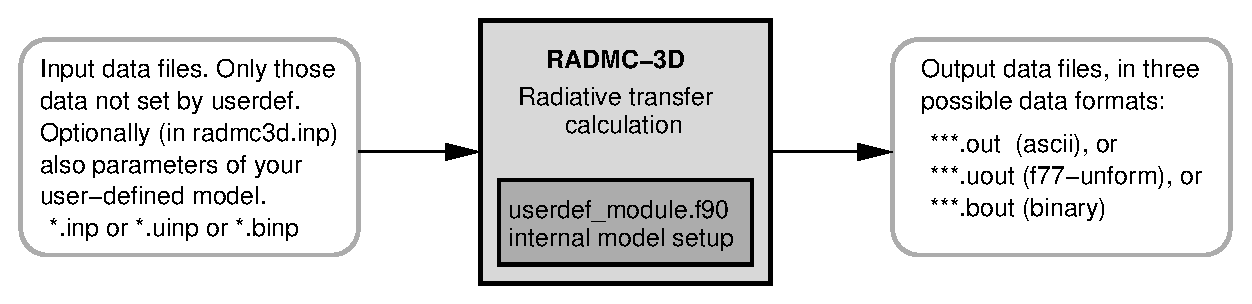
\includegraphics[height=0.13\textwidth]{dataflow_basic_userdef.eps}}
\caption{\label{fig-dataflow-basic-userdef}
Pictographic representation of the dataflow for the case when you 
define your model {\em internally} using the {\small\tt userdef\_module.f90}. 
}
\end{figure}
%

Often you still want some of the input data to be still read in in the usual
way, using input files. For instance, you may want to still read the
{\small\tt dustopac.inp} and the opacities using the {\small\tt
  dustkappa\_xxx.inp} files. This is all possible. Typically, you simply
keep the files you still want RADMC-3D to read, and omit the files that
contain data that you allocate and set in the {\small\tt
  userdef\_module.f90}. This is all a bit complicated, so the best way
to learn how to do this is to start from the example directories in which
a model is set up with the {\small\tt userdef\_module.f90} method.

In Fig.~\ref{fig-dataflow-basic-userdef} the dataflow for the user-defined
model setup is graphically depicted.

\section{The pre-defined subroutines of the userdef\_module.f90}
\label{sec-predef-userdef}
The idea of the {\small\tt userdef\_module.f90} is that it contains a number
of standard pre-defined subroutines that are called from the {\small\tt
  main.f90} code (and {\em only} from there). Just browse through the
{\small\tt main.f90} file and search for the sequence ``{\small\tt call
  userdef\_}'' and you will find all the points where these standard
routines are called. It means that at these points you as the user have
influence on the process of model setup. Here is the list of standard
routines and how they are used. They are ordered roughly in chronological
order in which they are called.
\begin{itemize}
\item {\small\tt userdef\_defaults()}\\
  This subroutine allows you to set the default value of any new parameters
  you may have introduced. If neither on the command line nor in the
  {\small\tt radmc3d.inp} file the values of these parameters are set, then
  they will simply retain this default value.
\item {\small\tt userdef\_commandline(buffer,numarg,iarg,fromstdi,gotit)}\\
  This subroutine allows you to add your own command-line options for
  {\small\tt radmc3d}. The routine has a series of standard arguments which
  you are not allowed to change. The {\small\tt buffer} is a string
  containing the current command line option that is parsed. You will check
  here if it is an option of your module, and if yes, activate it.  An
  example is listed in the code. You an also require a second argument, for
  which also an example is listed in the original code.
\item {\small\tt userdef\_commandline\_postprocessing()}\\
  After the command line options have been read, it can be useful to
  check if the user has not asked for conflicting things. Here you can
  do such checks.
\item {\small\tt userdef\_parse\_main\_namelist()}\\
  Here you can add your own namelist parameters that read from the
  {\small\tt radmc3d.inp} file. An example is provided in the original
  code.
\item {\small\tt userdef\_main\_namelist\_postprocessing()}\\
  Also here, after the entire {\small\tt radmc3d.inp} file has been read
  and interpreted, you can do some consistency checks and postprocessing
  here.
\item {\small\tt userdef\_prep\_model()}\\
  This routine can be used if you wish to set up the grid not from input
  files but internally. You will have to know how to deal with the
  {\small\tt amr\_module.f90} module. You can also set your own global
  frequency grid here. And finally, you can set your own stellar sources
  here. In all cases, if you set these things here (which requires you to
  make the proper memory allocations, or in case of the gridding, let
  the {\small\tt amr\_module.f90} do the memory allocations for you) 
  the further course of {\small\tt radmc3d} will skip any of its own
  settings (it will simply detect if these arrays are allocated already,
  and if yes, it will simply not read or allocate them anymore).
\item {\small\tt userdef\_setup\_model()}\\
  This is the place where you can actually make your own model setup.  By
  the time this subroutine is called, all your parameters have been read in,
  as well as all of the other parameters from the original {\small\tt
    radmc3d} code. So you can now set up the dust density, or the gas
  velocity or you name it. For all of these things you will have to allocate
  the arrays youself (!!!). Once you did this, the rest of the {\small\tt
    radmc3d} code won't read those data anymore, because it detects that the
  corresponding arrays have already been allocated (by you). This allows
  you to completely circumvent the reading of any of the following files
  by making these data yourself here at this location:
  \begin{itemize}
    \item {\small\tt amr\_grid.inp} or in the
      future the input files for any of the other griding types.
    \item {\small\tt dust\_density.inp}
    \item {\small\tt dust\_temperature.dat}
    \item {\small\tt gas\_density.inp}
    \item {\small\tt gas\_temperature.inp} 
    \item {\small\tt gas\_velocity.inp}
    \item {\small\tt microturbulence.inp}
    \item {\small\tt levelpop\_XXX.dat} 
    \item {\small\tt numberdens\_XXX.inp}
  \end{itemize}
  To learn how to set up a model in this way, we refer you for now to the
  {\small\tt ioput\_module.f90} or {\small\tt lines\_module.f90} and search
  for the above file names to see how the arrays are allocated and how the
  data are inserted. I apologise for not explaining this in more detail at
  this point. But examples are or will be given in the {\small\tt examples/}
  directory.
\item {\small\tt userdef\_dostuff()}\\
  This routine will be called by the main routine to allow you to do any
  kind of calculation after the main calculation (for instance after the
  monte carlo simulation). This is done within the execution-loop, so that
  if you use RADMC-3D in child mode, this routine will be called after each
  calculation. 
\item {\small\tt userdef\_myaction()}\\
  If RADMC-3D is called as {\small\tt radmc3d myaction}, then the
  user-defined routine {\small\tt userdef\_myaction()} is called, just like
  the spectrum making routine is called if you type {\small\tt radmc3d
    sed}. This allows the user to make RADMC-3D do special things on demand.
  Note that this can be used in combination with many of the above
  subroutines to interpret command-line options and {\small\tt radmc3d.inp}
  entries. {\em Not yet working in version 0.15.}
\item {\small\tt userdef\_compute\_levelpop()}\\
  This is a subroutine that can be called by the camera module for
  on-the-fly calculation of level populations according to your own recipe.
  This may be a bit tricky to use, but I hope to be able to provide some
  example(s) in the near future.  
\item {\small\tt userdef\_srcalp()}\\
  This subroutine allows you to add any emission/absorption process you
  want, even fake ones. For instance, you could use this to create nicely
  volume-rendered images of your 3-D models with fake opacities, which are
  chosen to make the image look nice and/or insight-giving.  You can also
  use this to add physical processes that are not yet implemented in
  RADMC-3D. This subroutine allows you full freedom and flexibility to 
  add emissivity and extinction whereever/however you like. To activate
  it you must set {\small\tt incl\_userdef\_srcalp = 1} in the
  {\small\tt radmc3d.inp} file. 
\item {\small\tt userdef\_writemodel()}\\
  This allows the user to dump any stuff to file that the user computed
  in this module. You can also use this routine to write out files that would
  have been used normally as input file (like {\small\tt amr\_grid.inp} or
  {\small\tt dust\_density.inp}) so that the IDL routines can read them if
  they need. In particular the grid information may be needed by these
  external analysis tools. Here is a list of standard subroutines you can
  call for writing such files:
  \begin{itemize}
    \item {\small\tt write\_grid\_file()}
    \item {\small\tt write\_dust\_density()}
    \item ...more to come...
  \end{itemize}
\item {\small\tt userdef\_reset\_flags()}\\
  If the user wants some flags to be reset after each command (in the
  child mode, see Chapter \ref{chap-child-mode}), then here it can be
  done.
\end{itemize}
For now this is it, more routines will be included in the future.

Note that the {\small\tt userdef\_compute\_levelpop()} subroutine, in
contrast to all the others, is called not from the {\small\tt main.f90}
program but from the {\small\tt camera\_module.f90} module. This is why the
camera module is the only module that is higher in compilation ranking than
the userdef module (i.e.\ the userdef module will be compiled before the
camera module). For this reason the userdef module has no access to the
variables of the camera module. For the rest, the userdef module has access
to the variables in all other modules.

Note also that not all input data is meant to be generated in this way. The
following types of data are still supposed to be read from file:
\begin{itemize}
  \item Dust opacity data
  \item Molecular fundamental data
\end{itemize}

Please have a look in the {\small\tt examples/} directory for models 
which are set up in this internal way.


\section{Some caveats and advantages of internal model setup}
\label{sec-internalsetup-proscons}
Setting up the models internally has several advantages as well as
disadvantages compared to the standard way of feeding the models into 
{\small\tt radmc3d} via files. The advantages are, among others:
\begin{itemize}
\item You can modify the model parameters in {\small\tt radmc3d.inp} and/or in
  the command line options (depending on how you allow the user to set these
  parameters, i.e.\ in the {\small\tt userdef\_parse\_main\_namelist()}
  routine and/or in the {\small\tt userdef\_commandline()} routine. You then
  do not need to run IDL anymore (except for setting up the basic files; see
  examples). Some advantages of this:
  \begin{enumerate}
  \item It allows you, for instance, to create a version of the {\small\tt
      radmc3d} code that acts as if it is a special-purpose model. You can
    specify model parameters on the command line (rather than going through
    the cumbersome IDL stuff).
    \item It is faster: even a large model is built up quickly and does not
      require a long read from large input files. 
  \end{enumerate}
\item You can make use of the AMR module routines such as the {\small\tt
    amr\_branch\_refine()} routine, so you can adaptively refine the grid
  while you are setting up the model.
\end{itemize}
Some of the disadvantages are:
\begin{itemize}
\item The model needs to be explicitly written out to file and read into IDL
  or any other data plotting package before you can analyze the density
  structure to test if you've done it right. You can explicitly ask
  {\small\tt ./radmc3d} to call the {\small\tt userdef\_writemodel()}
  subroutine (which is supposed to be writing out all essential data; but
  that is the user's responsibility) by typing {\small\tt ./radmc3d
    writemodel}.
\item Same is true for the grid, and this is potentially even more
  dangerous if not done. You can explicitly ask {\small\tt ./radmc3d} to
  write out the grid file by typing {\small\tt ./radmc3d writegridfile}.
  Note that if you call the {\small\tt write\_grid\_file()} subroutine
  from within {\small\tt userdef\_writemodel()}, then you do not have
  to explicitly type {\small\tt ./radmc3d writegridfile} as well.
  Note also that {\small\tt radmc3d} will automatically call the
  {\small\tt write\_grid\_file()} subroutine when it writes the
  results of the thermal Monte Carlo computation, if it has its
  grid from inside (i.e.\ it has not read the grid from the file
  {\small\tt amr\_grid.inp}.
\item It requires a bit more knowledge of the internal workings of the
  {\small\tt radmc3d} code, as you will need to directly insert code
  lines in the {\small\tt userdef\_module.f90} file. 
\end{itemize}


\section{Using the userdef module to compute integrals of $J_\nu$}
\label{sec-compute-radiation-integrals}
%
With the monochromatic Monte Carlo computation (see Section
\ref{sec-dust-monochromatic-monte-carlo}) we can calculate the mean
intensity $J_\nu$ at every location in the model at a user-defined set of
wavelengths. However, as mentioned before, for large models and large
numbers of wavelengths this could easily lead to a data volume that is
larger than what the computer can handle. Since typically the main
motivation for computing $J_\nu$ is to compute some integral of the
the form:
\begin{equation}
Q = \int_0^{\infty} J_\nu K_\nu d\nu
\end{equation}
where $K_\nu$ is some cross section function or so, it may not be
necessary to store the entire function $J$ as a function of $nu$.
Instead we would then only by interested in the result of this integral
at each spatial location. 

So it would be useful to allow the user to do this computation internally.
We should start by initializing $Q(x,y,z)=0$ (or $Q(r,\theta,\phi)=0$ if
you use spherical coordinates). Then we call the monochromatic Monte Carlo
routine for the first wavelength we want to include, and multiply the
resulting mean intensities with an appropriate $\Delta\nu$ and add this
to $Q(x,y,z)$. Then we do the  monochromatic Monte Carlo for the next
wavelength and again add to $Q$ everywhere. We repeat this until our
integral (at every spatial location on the grid) is finished, and we are
done. This saves a huge amount of memory.

Since this is somewhat hard to explain in this PDF document, we refer to
the example model {\small\tt run\_example\_jnu\_integral/}.

{\em STILL IN PROGRESS.}


\section{Some tips and tricks for programming user-defined subroutines}
Apart from the standard subroutines that {\em must} be present in the
{\small\tt userdef\_module.f90} file (see Section \ref{sec-predef-userdef}),
you are free to add any subroutines or functions that you want, which you
can call from within the predefined subroutines of Section
\ref{sec-predef-userdef}. You are completely free to expand this module as
you wish. You can add your own variables, your own arrays, allocate arrays,
etc. 

Sometimes you may need to know ``where you are'' in the grid. For instance,
the subroutine {\small\tt userdef\_compute\_levelpop()} is called with
an argument {\small\tt index}. This is the index of the current cell
from within which the subroutine has been called. You can now address,
for instance, the dust temperature at this location:
\begin{asciibox}\begin{verbatim}
temp = dusttemp(1,index)
\end{verbatim}\end{asciibox}
(for the case of a single dust species). You may also want to know 
the coordinates of the center of the cell. For this, you must first
get a pointer to the AMR-tree structure of this cell. The pointer 
{\small\tt b} is declared as
\begin{asciibox}\begin{verbatim}
type(amr_branch), pointer :: b
\end{verbatim}\end{asciibox}
Then you can point the pointer to that cell structure
\begin{asciibox}\begin{verbatim}
b => amr_index_to_leaf(index)%link
\end{verbatim}\end{asciibox}
And now you can get the x,y,z-coordinates of the center of the cell:
\begin{asciibox}\begin{verbatim}
xc = amr_finegrid_xc(b%ixyzf(1),1,b%level)
yc = amr_finegrid_xc(b%ixyzf(2),2,b%level)
zc = amr_finegrid_xc(b%ixyzf(3),3,b%level)
\end{verbatim}\end{asciibox}
Or the left and right cell walls:
\begin{asciibox}\begin{verbatim}
xi_l = amr_finegrid_xi(b%ixyzf(1),1,b%level)
yi_l = amr_finegrid_xi(b%ixyzf(2),2,b%level)
zi_l = amr_finegrid_xi(b%ixyzf(3),3,b%level)
xi_r = amr_finegrid_xi(b%ixyzf(1)+1,1,b%level)
yi_r = amr_finegrid_xi(b%ixyzf(2)+1,2,b%level)
zi_r = amr_finegrid_xi(b%ixyzf(3)+1,3,b%level)
\end{verbatim}\end{asciibox}

\section{Creating your own emission and absorption processes}
RADMC-3D Allows you to add your own physics to the ray-tracing images and
spectra. At every point during the ray-tracing process, when it computes the
emissivity and extinction coefficients $j_\nu$ and $\alpha_\nu$ it calls the
{\small\tt userdef\_srcalp()} subroutine, giving it the {\small\tt index} in
which cell we are, the frequencies of the different image channels and the
{\small\tt src} and {\small\tt alp} arrays which are for resp.\ $j_\nu$ and
$\alpha_\nu$. You can {\em add} any process by
\begin{asciibox}\begin{verbatim}
src(:) = src(:) + .....
alp(:) = alp(:) + .....
\end{verbatim}\end{asciibox}
where ...... is your formula. You can find the local variables like 
density and temperature using the {\small\tt index}, e.g.:
\begin{asciibox}\begin{verbatim}
rho_g = gasdens(index)
\end{verbatim}\end{asciibox}
You can be completely free in your choices. If you need some information
that is not usually read into RADMC-3D, you can add read commands in the
{\small\tt userdef\_setup\_model()} subroutine, e.g.:
\begin{asciibox}\begin{verbatim}
call read_gas_density(1)
\end{verbatim}\end{asciibox}

See the example directory {\small\tt examples/run\_simple\_userdefsrc} for
more ideas.

\section{Using RADMC-3D as a fancy volume-rendering tool}
Sometimes you want to make nice 3-D volume rendering images of e.g.\ your
3-D hydrodynamics simulation. You may, in that case, not be interested in
{\em real} emission/extinction processes, but rather some artificial
transfer function -- as long as the outcoming image looks nice. 

RADMC-3D offers a number of advantages over off-the-shelf programs for
volume rendering:
\begin{itemize}
\item It has AMR refinement, so you do not need to first convert into
  non-AMR grids which are necessary for many volume rendering codes.
\item It allows you full control over the transfer function, i.e.\ the
  dependence of the emission/extinction coefficients on any quantities
  such as density, temperature, magnetic field etc.
\end{itemize}

The example directory
\begin{asciibox}\begin{verbatim}
examples/run_simple_userdefsrc
\end{verbatim}\end{asciibox}
gives an example of how this can be done. It also shows how you can link
this to the {\small\tt viewimage.pro} routine, and allow on-the-fly
modification of the transfer function, so that you can experiment to get the
nicest image output.


%----------------------------------------------------------------------------
%               CHAPTER: USING THE IDL TOOL SET
%----------------------------------------------------------------------------
\chapter{Model analysis (I): The IDL model analysis tool set}
\label{chap-idl-analysis-tools}
%
While the code RADMC-3D is written in fortran-90, there is an extensive set
of tools written in IDL that make it easier for the user to set up models
and interpret results. See Section \ref{sec-install-idlscripts} for where
they are and how they can be properly installed so that they are easy to
use. Here we describe these tools. 


\section{The readradmc.pro tools}
\label{sec-readradmc}
%
The {\small\tt readradmc.pro} program file contains a series of subroutines for
reading RADMC-3D output into IDL so that the user can do post-processing and
analysis on these data. The file also contains subroutines for operating
RADMC-3D directly from within IDL. 

\subsection{Function readimage}
%
The {\small\tt readimage()} function reads the latest produced image into IDL.
This image is (i.e.\ should be) located in the file {\small\tt image.out}, which
is produced by RADMC-3D. The {\small\tt readimage()} function returns an IDL
structure containing the image (be it a single-frequency image or a
multi-frequency image) in units of intensity (erg/s/cm$^2$/Hz/ster), as
well as information about the pixel grid and at which frequency(ies) the
image was taken. With the ``help'' command you can see the full
contents of the returned structure:
\begin{asciibox}\begin{verbatim}
.r readradmc.pro
a=readimage()
help,a,/str
\end{verbatim}\end{asciibox}
This will show you the contents of the structure. Here is a quick summary
of these contents:
\begin{itemize}
\item[] {\small\tt nx, ny}: The number of pixels in x- and y- direction in the image
\item[] {\small\tt nrfr}: The number of frequencies (wavelengths), i.e.\ the number of images at different wavelengths
\item[] {\small\tt sizepix\_x, \_y}: The size of the pixels in x- and y-
  directions in units of centimeters. This is of course only possible for
  images at semi-infinity (the default). For images made as a local
  observer, see Section \ref{sec-local-observer} for details.
\item[] {\small\tt image}: The nx$\times$ny array of intensities of the image.
  If multiple colors (wavelengths, frequencies) are present, then the
  {\small\tt image} array will be three-dimensional:  nx$\times$ny$\times$nrfr.
  The intensities are in units of erg/cm$^2$/s/Hz/ster.
\item[] {\small\tt flux}: The integral of the intensity over the entire image,
  i.e.\ the flux in the image. The units are erg/cm$^2$/s/Hz for an 
  observer at 1 parsec distance. This ``1 parsec'' is just a normalization
  distance. If you make images of objects much larger than 1 parsec in size,
  this does {\em not} mean that the image is made by a local observer (unless
  explicitly specified, see Section \ref{sec-local-observer}). It is just
  so that you can compute the actually observed flux by multiplying the flux
  by a factor $(\mathrm{pc}/d)^2$, where $d$ is the true distance of the 
  observer (which must then be much larger than the size of the object to
  keep the far-field limit valid).
\item[] {\small\tt x,y}: The actual image coordinates in cm (unless local
  observer, see Section \ref{sec-local-observer}). These are in principle
  redundant because you can calculate them yourself from the 
  {\small\tt sizepix\_x, \_y} and {\small\tt nx, ny} values. They are here just for
  convenience.
\item[] {\small\tt lambda}: The wavelength (in micron) at which this image was
  made. For multiple colors/freqs/wavelengths this is an array.
\end{itemize}
The {\small\tt readimage()} function can also be used to read from a pipe between
IDL and RADMC (see ``child mode'' in Chapter \ref{chap-child-mode}). One
then gives it as an argument the file number of the pipe (see example shown
in Chapter \ref{chap-child-mode}). This is in fact what is done by {\small\tt
  viewimage.pro} below.


\subsection{Subroutine plotimage}
%
The subroutine {\small\tt plotimage} plots the image read by {\small\tt readimage()} to
screen (or postscript file) in a proper way. Check out the following 
example (to be executed only after the dust temperatures have been
written to file {\small\tt dust\_temperature.dat}):
\begin{asciibox}\begin{verbatim}
.r readradmc.pro
a=readimage()
plotimage,a,/au
\end{verbatim}\end{asciibox}
This subroutine is in fact used by the {\small\tt viewimage.pro} below to display
images on the drawing pane of the GUI widget. The {\small\tt plotimage} subroutine
has a large number of optional arguments:
\begin{itemize}
\item[] {\small\tt /au} or {\small\tt /pc}: Display spatial scales in units of AU or parsec.
\item[] {\small\tt /log}: Display the image using logarithmic spacing of the
  brightness levels. This allows you to gain far greater depth in the image.
\item[] {\small\tt /contour}: Overplot contours over the image
\item[] {\small\tt nlevels}: Number of levels for the contours
\item[] {\small\tt /noimage}: If set, only plot axes
\item[] {\small\tt position}: An array of 4 numbers specifying position of plot on
  the canvas. Like position keyword in typical IDL plotting routines.
\item[] {\small\tt maxlog}: Set the maximum number of factors of 10 the log
  brightness color coding will span
\item[] {\small\tt saturate}: Allows you to enhance the contrast of very weak
 emission regions by saturating bright regions
\item[] {\small\tt /jpg}: Write the image to a JPEG file
\item[] {\small\tt lgrange}: A two-valued array specifying the range in brightness 
  (in 10-log) that the image will show
\item[] {\small\tt filenr}: (For case of /jpg): if set to e.g. 6 it will write the
  JPEG image to file {\small\tt image\_6.jpg}. 
\item[] {\small\tt ilam}: If the image is a multi-color image, ilam specfies
  which of the images you wish to plot
\item[] {\small\tt coltune}: If set to 1, then rescale the brightness of all
  channels the same value, to get the best color depth. If set to a
  3-element array, you can directly specify the weight of each color.  In
  this way you can really fine-tune the colors.
\item[] {\small\tt zoom}: If set to a 4-valued array, it makes {\small\tt plotimage} put
  the proper x- and y- axis scaling for the particular zoom-in. Normally the
  center of the image is taken to be $(0,0)$, but with this zoom keyword you
  can set exactly what the x- and y-axes should display. Warning: it
  overrides the pixel size specifications in the image. 
\end{itemize}


\subsection{Subroutine makeimage}
\label{sec-idl-makeimage}
%
The subroutine {\small\tt makeimage} allows the user to interact with RADMC-3D for
making images in an easy way, although a direct calling of the {\small\tt radmc3d}
command with the corresponding keywords is almost just as easy. So one can
also consider this as an example routine for calling RADMC-3D for making
images. From within IDL you can call makeimage as follows:
\begin{asciibox}\begin{verbatim}
makeimage,incl=34.,phi=40.,lambda=11.3
\end{verbatim}\end{asciibox}
Here are the keywords:
\begin{itemize}
\item[] {\small\tt incl}: The inclination of the object on the sky of the
  observer.  {\small\tt incl}=0 means a view from the northpole downward, {\small\tt
    incl}=180 means a view from the southpole upward and {\small\tt incl}=90 means
  an edge-on view.
\item[] {\small\tt phi}: The rotation of the object along its z-axis. A positive
  {\small\tt phi} means that the object rotates counter-clockwise, i.e. that the
  observer rotates clockwise around the object.
\item[] {\small\tt npix}: Number of pixels (assumed to be the same for x and y)
\item[] {\small\tt sizecm / sizeau / sizepc}: The size of the image in units of
  centimeter / AU / parsec. The size means the full width and full height of
  the square image. 
\item[] {\small\tt posang}: The rotation of the image in the image plane, i.e.\
  the position angle of the image on the sky. Default is 0.
\item[] {\small\tt nofluxcons}: If set to 1 ({\small\tt /nofluxcons}) we use the fast
  ray-tracing method, while if not set (default) we use the accurate method
  with sub-pixeling for flux conservation (see Section \ref{sec-image-refinement}).
\item[] {\small\tt pointcm / pointau / pointpc}: A three-valued array giving the
  3-D coordinates of the point toward which we aim our camera. Default is
  (0.,0.,0.). Units are cm / AU / parsec.
\item[] {\small\tt ifreq}: If specifying {\small\tt ifreq} (putting it to an integer
  value of 1 or higher) then the wavelength at which the image is going to
  be taken is taken from the global frequency array from the 
  {\small\tt wavelength\_micron.inp} file. The integer {\small\tt ifreq} is then the
  index of the wavelength you want to use. Note that this integer starts
  with 1 (fortran convention). 
\item[] {\small\tt lambda}: If {\small\tt lambda} is specified, this will be the
  wavelength at which the image is to be taken. This wavelength does not
  have to be part of the global frequency array. It can be any value, even a
  value in between wavelength grid points of the dust opacity files or
  so. In that case, a linear interpolation of these opacities will then
  allow RADMC-3D to nevertheless make the image. So any positive value of
  {\small\tt lambda} is allowed. NOTE: You cannot specify both {\small\tt lambda} and
  {\small\tt ifreq} simultaneously.
\item[] {\small\tt nostar}: If set, then the star(s) in the model are not included
  in the images. 
\item[] {\small\tt zoomau / zoompc}: Specify the precise window on the image plane
  which you like to zoom in to. Note that $(0.,0.)$ is the location in the
  image plane that points to the pointing location specified by 
  {\small\tt pointcm / pointau / pointpc}.
  NOTE: You cannot specify both {\small\tt sizecm / sizeau / sizepc} and 
  {\small\tt zoomau / zoompc} simultaneously.
\item[] {\small\tt plottau}: If set to 1, the images will not show the emission
  at that wavelength but instead the total integrated optical depth of the
  ray at that wavelength. This is only useful for debugging purposes.
\item[] {\small\tt iounit}: For child mode (See chapter \ref{chap-child-mode}).
\end{itemize}

NOTE: If you want to make multiple images of the same object, then it may be
much too slow if each time a new image is to be taken, the RADMC-3D code
must be restarted and the entire model must be re-read into RADMC-3D. You
can use RADMC-3D in "child mode" to have it start up just once (and reading
all input data just once) and keeping alive until explicitly told to end. 
By communicating with it via a pipe you can then quickly get your images
one-by-one while having the slow I/O only once. You do this by starting
RADMC-3D in the way described in Chapter \ref{chap-child-mode}, and then
calling {\small\tt makeimage} with keyword {\small\tt iounit} equal to the unit of
the pipe. See chapter \ref{chap-child-mode} for an example.

\subsection{Subroutine read\_data()}
\label{sec-idl-read-data}
%
It is always useful to analyze the dust temperature structure that RADMC-3D
produces. The function {\small\tt read\_data()} (or {\small\tt readdata()}
in abbreviated form) is meant to do that. In IDL, the way it works is:
{\small\begin{verbatim}
.r readradmc
a=read_data(/dtemp)
\end{verbatim}}
The {\small\tt /dtemp} stands for ``read the dust temperature''. You can
also read the dust density (which is an input, not an output of RADMC-3D):
{\small\begin{verbatim}
a=read_data(/ddens)
\end{verbatim}}
You can find what is contained in the structure {\small\tt a} by
{\small\begin{verbatim}
help,a,/struct
\end{verbatim}}
The structure {\small\tt a} contains a sub-structure {\small\tt grid}:
{\small\begin{verbatim}
help,a.grid,/struct
\end{verbatim}}
which contains all the information of the grid. We come back to that
later.

If you just read the dust temperature (with {\small\tt /dtemp}) then you
can see that the structure contains a large array called {\small\tt a.temp}.
Its dimensionality depends on which kind of grid you are using:
\begin{itemize}
\item {\em Regular grid:}\\ The array {\small\tt a.temp} (or any other data
  array) will have dimensions {\small\tt a.temp(nx,ny,nz,nspec)}, where
  {\small\tt nx,ny,nz} are the number of cells in x, y and z direction and
  {\small\tt nspec} is the number of dust species. If {\small\tt nspec=1},
  then the array automatically becomes {\small\tt a.temp(nx,ny,nz)} (this is
  IDL convention).
\item {\em Oct-tree AMR grid:}\\ The array {\small\tt a.temp} (or any other
  data array) will have dimensions {\small\tt a.temp(ncells,nspec)}, where
  {\small\tt ncells} is the number of real cells (excluding the branches
  that are divided into subcells: only the leafs count) in the AMR oct-tree.
  How the (complex!) oct-tree is structured is specified in {\small\tt
    a.grid}. The {\small\tt nspec} is again the number of dust species.
\item {\em Layer-style AMR grid:}\\ The array {\small\tt a.temp} (or any other
  data array) will have dimensions {\small\tt
    a.temp(nxmax,nymax,nzmax,nspec,nlayers+1)}, where {\small\tt
    nxmax,nymax,nzmax} are the maximum of number of cells in x, y and z
  direction of all the layers (including the base grid). The {\small\tt
    nspec} is again the number of dust species. The {\small\tt nlayers} is
  the number of refinement layers (patches), where 0 means that there is
  only the base grid, 1 means there is one single patch of refinement, etc.
  The last index of the {\small\tt a.temp} array goes from 0 to
  {\small\tt nlayers}. Here 0 means the base grid, 1 the first layer of
  refinement, etc. Note that if you just read the dust temperature in 
  this way, the regions in the parent layers (including the base grid)
  that are replaced by a refined layer will have the value 0. This makes
  a ``hole'' in the dust temperature distribution. If you want IDL to
  fill these holes with the rebinned values of the refined layers, then
  you can call {\small\tt read\_data} with the {\small\tt /fill} keyword,
  i.e.\ {\small\tt read\_data(/dtemp,/fill)}.
\end{itemize}

Now coming back to the {\small\tt a.grid} sub-structure. This contains
all the information about the grid. Again the content of this structure
depends on which gridding you use:
\begin{itemize}
\item {\em Regular grid:}\\ The structure contains {\small\tt x,y,z} which are
  1-dimensional arrays with the cell-centered x, y and z coordinates (for
  spherical coordinates they are $r$, $\theta$ and $\phi$, but then the grid
  also contains, for your convenience, the entries {\small\tt r}, {\small\tt
    theta} and {\small\tt phi}). It also contains {\small\tt xi,yi,zi} which
  are again 1-D arrays with the x, y and z coordinates of the cell walls
  (for spherical coordinates {\small\tt ri}, {\small\tt thetai} and
  {\small\tt phii}). {\small\tt nx, ny, nz} are the number of cells in 
  x, y and z direction.
\item {\em Oct-tree AMR grid:}\\ The {\small\tt x,y,z} and {\small\tt
    xi,yi,zi} (and in addition to that in spherical coordinates {\small\tt
    r}, {\small\tt theta}, {\small\tt phi}, {\small\tt ri}, {\small\tt
    thetai} and {\small\tt phii}) still have the same meaning as in the
  regular grid case. In this case, however, this ``regular grid'' is just
  the ``base grid'' of the oct-tree refinement. The oct-tree structure is
  now specified by the 1-D byte-array {\small\tt octtree}, which contains
  only the values 0 and 1. See Section \ref{sec-grid-input} for details
  about their meaning. The order of the values of the data are the same
  as the order of the cells given by {\small\tt octtree}.
\item {\em Layer-style AMR grid:}\\ Again, as in the oct-tree case, the
  {\small\tt x,y,z} and {\small\tt xi,yi,zi} and their spherical-coordinates
  counterparts now have their meaning for the base grid. The {\small\tt
    nlayers} tells how many layers (in addition to the base grid) there
  are. The {\small\tt iparent(nlayers+1)} give the parent layer for each
  layer, where 0 means base grid. The {\small\tt ixyz(3,nlayers+1)} give the
  starting point of the layer in the parent grid, {\small\tt
    nxyz(3,nlayers+1)} the size of the layer in the parent grid and
  {\small\tt nnxyz(3,nlayers+1)} the size of the layer in its own grid.  The
  {\small\tt layer\_x(nxmax,nlayers+1)}, {\small\tt
    layer\_y(nxmax,nlayers+1)}, {\small\tt layer\_z(nxmax,nlayers+1)},
  {\small\tt layer\_xi(nxmax,nlayers+1)}, {\small\tt
    layer\_yi(nxmax,nlayers+1)} and {\small\tt layer\_zi(nxmax,nlayers+1)}
  are like the {\small\tt x,y,z} and {\small\tt xi,yi,zi}, but now for each
  layer separately. Note that e.g.\ {\small\tt layer\_x[*,0] = x[*]}, etc,
  because layer 0 is identical to the base grid. Note also that 
  {\small\tt ixyz[*,0]} and {\small\tt nxyz[*,0]} have no meaning, but
  {\small\tt nnxyz[*,0]} are the same as {\small\tt nx, ny, nz}. 
\end{itemize}
For all the above griddings, the following additional elements are present
in {\small\tt a.grid}. For instance, {\small\tt gridstyle (=0,1,10)}
specifies which of the above griddings is used, {\small\tt coordsys} is the
coordinate system, {\small\tt mirror (=0,1)} a flag whether equatorial
mirror symmetry is present (only for spherical coordinates), {\small\tt
  ncell} gives you the total number of actual cells, {\small\tt ncellinp}
gives you the total number of read-in cell values (in case of layer-type
refinement this is generally larger than {\small\tt ncell}, {\small\tt incx,
  incy, incz (=0,1)} are flags whether the x, y or z dimensions are active
or not.

Note that even if you have e.g.\ a regular grid, the {\small\tt ixyz} etc
elements are still in the structure, but they are simply 0.



\section{Support for FITS}
\label{sec-fits-support}
%
Many people in astronomy use the FITS format (Flexible Image Transport
System) for analyzing images or other observational data. Many software
packages are geared toward reading and processing FITS data. For instance,
the {\small\tt ds9} image viewer\footnote{{\footnotesize\tt http://hea-www.harvard.edu/RD/ds9/}}
is very powerful, but requires its images in FITS format.

We provide a conversion routine from the standard {\small\tt image.out}
image format produced by RADMC-3D to FITS format. The routine is called
{\small\tt radmcimage\_to\_fits} and is located in the file {\small\tt
  idl/radmc3dfits.pro}. To use this, you must have the ASTROLIB
\footnote{{\footnotesize\tt http://idlastro.gsfc.nasa.gov/}} library of IDL
installed.

To convert to FITS format, you must specify the distance at which the
observer stands from the object. The reason is that the {\small\tt image.out}
file produced by RADMC-3d is {\em distance independent!} The pixel size
in {\small\tt image.out} is specified in centimeters, not as an angular
size. The {\small\tt radmcimage\_to\_fits} routine automatically converts 
this to pixel scale in degrees, but it must know the distance. 

Here is how you convert {\small\tt image.out} into {\small\tt image.fits}.
First go into IDL and then:
\begin{asciibox}\begin{verbatim}
.r radmc3dfits
radmcimage_to_fits,'image.out','image.fits',140.
\end{verbatim}\end{asciibox}
where the last number (140.) is the distance to the object in units of
parsec. In the FITS file the unit of the intensity is Jansky/Pixel. The
pixel sizes are specified in degrees. Once you have made this conversion,
you can, for instance, use {\small\tt ds9} (if it is installed on your
system!) to view your image. From the unix shell you type:
\begin{asciibox}\begin{verbatim}
ds9 image.fits
\end{verbatim}\end{asciibox}

Just for your information, in case you want to know more about 
the FITS conversion: The FITS header looks for example like this:
\begin{asciibox}\begin{verbatim}
SIMPLE  =                    T /image conforms to FITS standard                 
BITPIX  =                  -64 /bits per data value                             
NAXIS   =                    2 /number of axes                                  
NAXIS1  =                  100 /                                                
NAXIS2  =                  100 /                                                
EXTEND  =                    T /file may contain extensions                     
BTYPE   = 'Intensity'                                                           
BUNIT   = 'JY/PIXEL'                                                            
CDELT1  =  6.9418601352850E-07                                                  
CUNIT1  = 'deg     '                                                            
CRPIX1  =  5.0000000000000E+01                                                  
CDELT2  =  6.9418601352850E-07                                                  
CUNIT2  = 'deg     '                                                            
CRPIX2  =  5.0000000000000E+01                                                  
RESTFREQ=   2.997924580000E+13                                                  
END                                                                             
\end{verbatim}\end{asciibox}
which you can see if you type {\small\tt less image.fits} in the Unix shell and
rescale the width of your shell window to 80 characters. If you want to know
more about the details of the FITS format, please consult the various 
papers by E.W.~Greisen, for instance Greisen \& Calabretta (2002) A\&A
395, 1061-1075.


\section{The image viewing GUI: viewimage}
\label{sec-viewimage-gui}
%
Making images of a model can be done ``by hand'' using the tools in the
{\small\tt readradmc.pro} file (see Section \ref{sec-readradmc}). But it is
much more convenient to use the fully widget-based graphical user interface
{\small\tt viewimage} (see Fig.~\ref{fig-gui-screenshot})\footnote{\em
  NOTE: Currently there appears to be a problem that viewimage will freeze,
  which happens on some machines and not on other machines (in fact it
  happened on one Macbook but not on another, while the systems were
  seemingly identical). This is somehow related to the way radmc3d and IDL
  communicate with each other in child mode (see chapter
  \ref{chap-child-mode}): it must be a buffering problem. So far I could not
  figure out what is going wrong, but I will continue to work on this. If
  you experience this problem, try calling viewimage,/nochild. That is
  slower, but should work.}.

{\bf Important notice:} As of version 0.38 of RADMC-3D there is not only the
original IDL-version of the viewimage tool ({\small\tt viewimage.pro}) but
also a new version that is not dependent on having an IDL-license: it is a
stand-alone package written by Farzin Sereshti and uses the Qt
cross-platform widget library\footnote{\url{http://qt-project.org}}. You can
find this version in the {\small\tt viewimage\_QT\_GUI/} directory.

This interface can be used once the dust temperatures (in case of dust
continuum radiative transfer) have been computed using e.g.\ the thermal
monte carlo method (i.e.\ after having called {\small\tt radmc3d mctherm}).
Or more precisely: the file {\small\tt dust\_temperature.dat} should be
present and consistent with the other files. If this is satisfied, then one
can go into IDL (does not work on the IDL-clone ``GDL'') and type:
\begin{asciibox}\begin{verbatim}
.r viewimage
viewimage
\end{verbatim}\end{asciibox}
and one should get the GUI shown in
Fig.~(\ref{fig-gui-screenshot}). Alternatively (if you don't have an IDL
license) you install the Qt-version of the viewimage (in the {\small\tt
  viewimage\_QT\_GUI/} directory; there is an extensive manual for that tool
in that directory). {\em NOTE: It may take a while for RADMC-3D to load all
  the data into memory the first time, so before the first image appears on
  the screen it may take some time.  From that point on, further ray-trace
  actions should go much quicker}.  Here is a list of controls and their
functions:
\begin{itemize}
\item {\small\tt ``Quit Viewer'' button:} Ends this viewer and quits RADMC-3D.
\item {\small\tt ``Write Image'' button:} Writes a idl.ps postscript version of
  the plot on the screen.
\item {\small\tt ``mouse rotate'' switch:} If unset (default), the mouse clicks
  on the plotting pane act to select a zoom-in box. If set, the mouse clicks
  on the plotting pane act to rotate the object. Note that the rotation can
  also be done by hand by setting the values of {\small\tt ``Inclination''} and
  {\small\tt ``Phi''} and redoing an image rendering with the {\small\tt ``Render
    Image''} button.
\item {\small\tt ``lin'' switch:} Switch between linear color table of intensity
  and logarithmic color table of intensity. 
\item {\small\tt ``preview'' switch:} If set (default) then the ray-traced image
  is done without sub-pixeling in regions where the model has higher spatial
  resolution than the image resolution can resolve. This is a fast mode (i.e.
  hence the name ``preview''). If unset, then the ray-tracer always ensures
  that if a pixel of the image does not resolve details of the model, it will
  internally refine the pixel in 2x2 (and recursively repeat this until the
  resolution matches that of the model), and finally integrate the flux of
  all the sub-pixels to find the flux of the parent pixel. The intensity it
  then puts into this pixel is then the true average intensity over all the
  pixel. The sub-pixels will never be seen by the user. They are only made
  internally in RADMC-3D to ensure the correct flux in the pixel, and then
  dropped again. For science-quality images the {\small\tt ``preview''} button
  should be unset. It may take longer, however, to render. Please read 
  Section \ref{sec-image-refinement} for details about this procedure.
\item {\small\tt ``contour'' switch:} If set: overplot contours.
\item {\small\tt ``star'' switch:} If set (default): Include the flux of all the
  point-source stars in the image. Not setting it has the potential
  advantage that you can concentrate on the circumstellar material and not 
  be 'blinded' by the strong starlight.
\item {\small\tt slider in this box:} The slider in the same box as the above
  switches selects the IDL color table for monochromatic images.
\item {\small\tt ``MaxLog'' textbox (editable):} The maxlog is the maximum number of factors of
  10 that we will include in the color table. A high number gives more
  extreme ``depth'' to the image, but may also wash out details.
\item {\small\tt ``Saturate'' textbox (editable):} Saturate the image with this
  factor. Default is 1.0, i.e.\ no saturation.
\item {\small\tt ``Nr Cont'' textbox (editable):} Set how many contours you want
  if the contour switch is 'on'.
\item {\small\tt ``Render Spectrum'' button:} Render a complete SED. This may take
  a long time!
\item {\small\tt ``Render Image'' button:} Render a single image. See entries below
  for the settings.
\item {\small\tt ``Unzoom'' button:} If you are zoomed in, and you want to zoom out
again, push this button. Note: Zoomin in is done by selecting a region with the
moise in the image pane (make sure the ``mouse rotate'' switch is off) and
pressing {\small\tt ``Render Image''}. 
%
\begin{figure}
\centerline{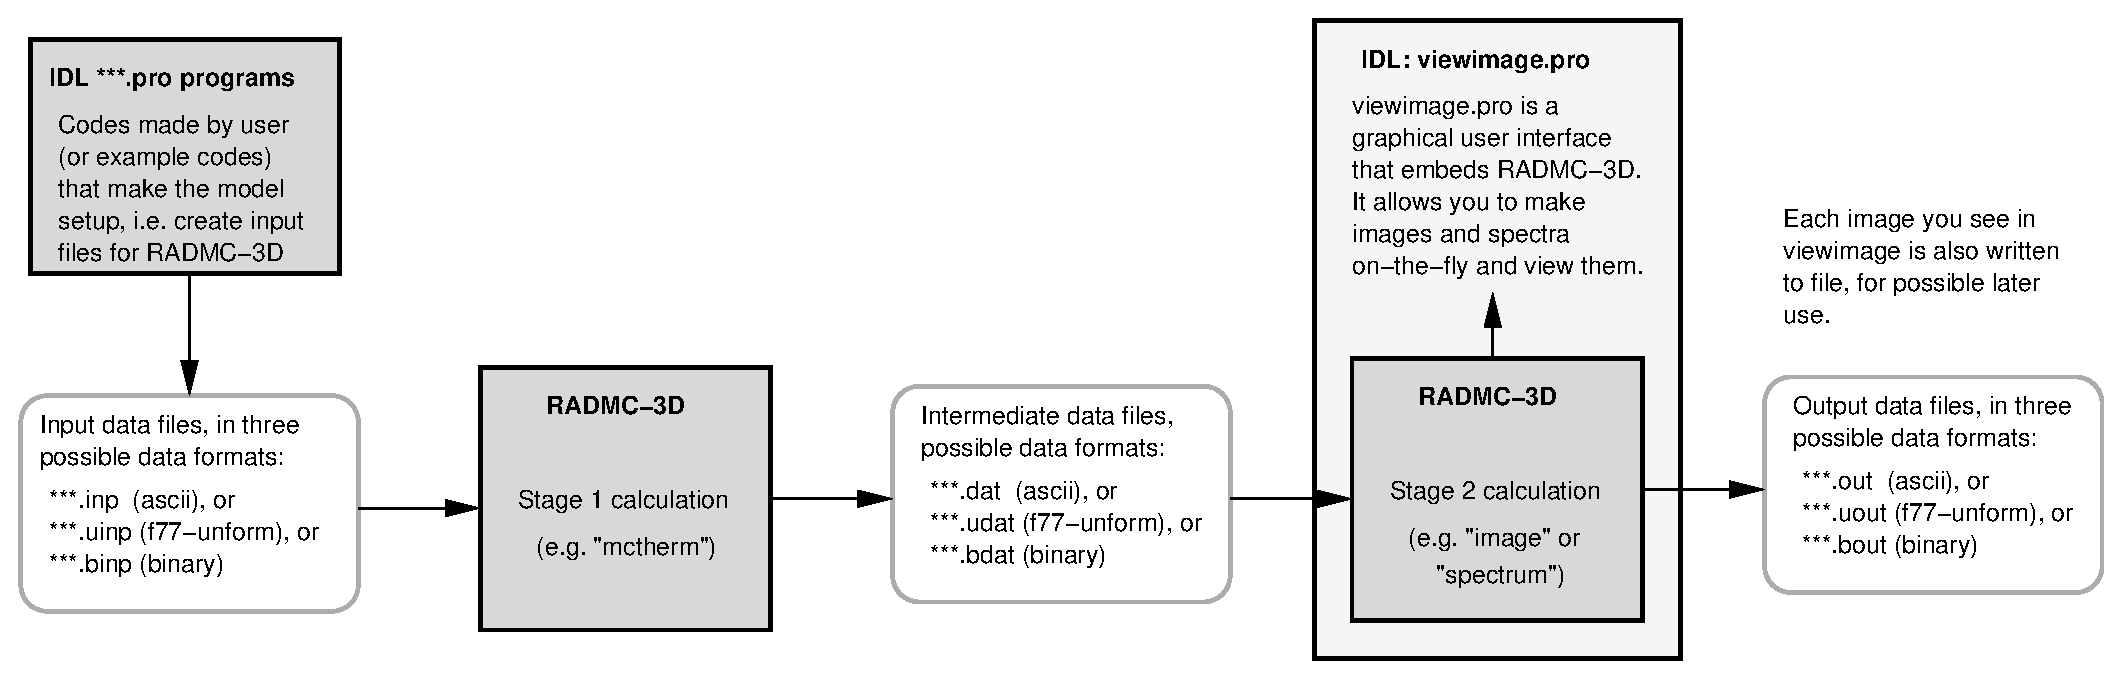
\includegraphics[height=0.32\textwidth]{dataflow_viewimage_twostage.eps}}
\caption{\label{fig-dataflow-viewimage-twostage} Pictographic representation
  of the dataflow of RADMC-3D when the {\small\tt viewimage} GUI is
  used. RADMC-3D is then called from within {\small\tt viewimage}.  Note
  that the two-stage procedure is shown here, e.g.\ when dust temperatures
  are computed in stage 1. Only the imaging stage (stage 2) is done by the
  {\small\tt viewimage}-{\small\tt radmc3d} symbiosis. In case of
  single-stage procedures (e.g.\ LTE line transfer with a given temperature)
  we go straight from the {\small\tt .inp} files via {\small\tt
    viewimage}-{\small\tt radmc3d} to the image in the GUI.}
\end{figure}
%
\item {\small\tt ``Npix'' textbox (editable):} The number of x and y pixels of the
  image.
\item {\small\tt ``Size'' textbox (editable):} The size of the image.
{\bf [BUG HERE: This does not seem to work.]}
\item {\small\tt ``Inclination'' textbox (editable):} The inclination where the
  observer is placed (at large distance).
\item {\small\tt ``Phi'' textbox (editable):} The azimuthal angle where the
  observer is placed (at large distance). 
\item {\small\tt slider below:} The wavelength slider. These are the wavelengths
  from the {\small\tt wavelength\_micron.inp} file and using the slider you can
  select one of these values. BUT: you can also select the wavelength by
  directly editing the textbox next to it, see below.
\item {\small\tt textbox next to slider:} The current wavelength in micron. This
  is automatically set when the slider is moved. BUT you can also put in 
  any value of the wavelength you want and type return to get the image at
  the precise wavelength of interest. That may be a wavelength that is not
  one of the {\small\tt wavelength\_micron.inp} values, but somewhere in between
  or even outside that grid. You can try any value. 
\end{itemize}
%
\begin{figure}
\centerline{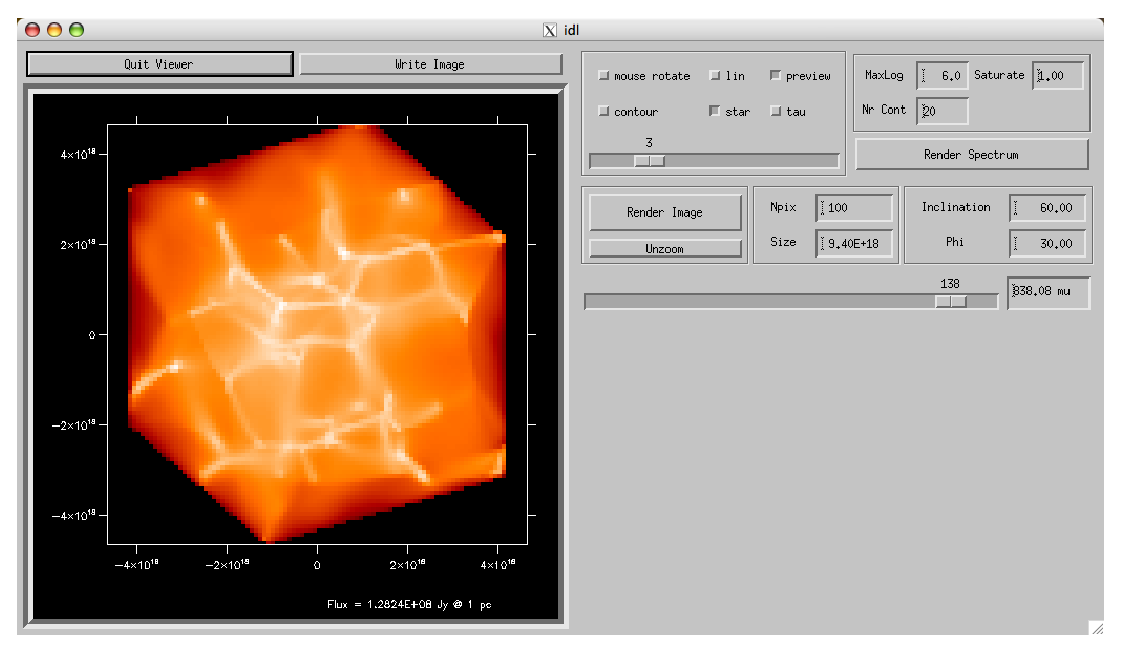
\includegraphics[width=0.9\textwidth]{gui.eps}}
\caption{\label{fig-gui-screenshot}
The graphical user interface (GUI) to the ray-trace-based imager
module of RADMC-3D. NOTE: As of version 0.38 we now have also 
a non-IDL version of viewimage using the Qt library.}
\end{figure}
%

The image is of course independent of observer distance (except for the
local observer mode). The total flux, however, is a distance-dependent
quantity. Written in the image is the total flux, normalized to a distance
of 1 parsec. Clearly, if the model is far bigger than 1 parsec, then this
number has no physical meaning. But by scaling the image flux to a reasonale
distance you will get reasonable answers.

The {\small\tt viewimage} routines will print to the command line the {\small\tt radmc3d} 
command sequence used to make the image you see now on your screen. This is
just for the user's convenience, that it is clearly seen which commands
{\small\tt radmc3d} receives. You can simply copy-paste such a line to the
shell command line and you will see that RADMC-3D will do precisely that
command (note that if already another RADMC-3D is running a huge model,
you may get memory problems when doing this in parallel to that model). 

Note also that each time a new image is made and is shown in the viewer, the
same image is also stored in the file {\small\tt image.out} in the current
directory. This means that you can read the latest image using the
{\small\tt readimage()} routine in the {\small\tt readradmc.pro} file. As
an example of such a complete sequence:
\begin{asciibox}\begin{verbatim}
.r viewimage
viewimage
<<< NOW MAKE WITH THIS WIDGET SOME NICE IMAGE YOU WANT TO STUDY MORE >>> 
.r readradmc
a=readimage()
window,0
surface,a.image
\end{verbatim}\end{asciibox}
In this example you make a surface plot in window 0 of the image you see in
the viewer.

There are further capabilities of {\small\tt viewimage}, which can be switched
on with keyword options to the {\small\tt viewimage} subroutine. Here is a list
of such keyword options (i.e.\ type e.g.\ {\small\tt viewimage,/color} to 
enable the first option):
\begin{itemize}
\item[] {\small\tt /color}: When {\small\tt /color} is set then you will find three
  wavelength sliders which can be independently shifted. These three sliders
  represent the red, green and blue channels of the image. This way you
  can make false color images.
\item[] {\small\tt /au / /pc}: When setting either {\small\tt /au} or {\small\tt /pc} the axis
  will not be drawn with centimeter units, but instead with AU or parsec
  units.
\item[] {\small\tt /small}: If set, the widget will be smaller, so that it fits
  on low-resolution screens.
\item[] {\small\tt /verti}: If set, the widget will put the controls below the
  image instead of next. Can be useful on high-resolution screens to save
  screen real estate.
\item[] {\small\tt /nochild}: When setting {\small\tt /nochild}, the RADMC-3D code will
  be called separately for each image rendering. This can be very slow, but
  it has the advantage that in case of problems the debugging might be
  easier, because all I/O of the {\small\tt radmc3d} executable will then go to
  screen.
\item[] {\small\tt /lines}: This includes entry fields such as {\small\tt imol},
  {\small\tt iline} and {\small\tt vkms} to make it easier to specify the 
  precise wavelength of the image in case of lines.
\end{itemize}

{\em Tip: If viewimage unexpectedly quits or freezes, please have a look at
  the file} {\small\tt radmc3d.out} {\em which contains the messages that
  RADMC-3D outputs. This may give hints what went wrong. If you have called
viewimage with the option /nochild, then the output will have been written
to screen, not to} {\small\tt radmc3d.out}.

Another thing to keep in mind is that when RADMC-3D makes images, it will
run a small Monte Carlo simulation beforehand to compute the scattering
source function (see ).

\section{Making and reading spectra with IDL}
\label{sec-spectra-from-idl}
%
{\bf [THIS STILL HAS TO BE WRITTEN]}




\section{A general-purpose 3-D datacube analysis GUI}
\label{sec-render3d}
Although this is not specific for RADMC-3D, we thought it would anyway be
useful to provide this: a super-fast interactive IDL GUI for analyzing 3-D
data cubes called {\small\tt render3d.pro}. This code is a general-purpose
adaption of one of IDL's example codes, so this is not in any way
copyrighted by the RADMC-3D authors, even though we made extensive changes
to it for the better. The tool can be used also for any other 3-D datacube
data: it is not at all limited to RADMC-3D. 

The {\small\tt render3d.pro} tool can only handle 3-D regularly spaced
data. No AMR-based models can be {\em directly} analyzed in this way. But
in Chapter \ref{chap-radmc3d-internal-analysis-tools} we describe a feature
of the {\small\tt radmc3d} code that allows you to easily create 3-D regularly
spaced boxes from anywhere in your model at any spatial resolution you like.
You can then subsequently feed that datablock into {\small\tt render3d.pro}
for 3-D viewing. 

Using {\small\tt render3d.pro} is simple:
\begin{asciibox}\begin{verbatim}
q = <some 3-D array of floats or double precisions>
.r render3d
render3d,q
\end{verbatim}\end{asciibox}
Have fun! For all the functionality, just try things out. It should be
reasonably self-explanatory. See Fig.~\ref{fig-render3d} for a screen-shot.
%
\begin{figure}
\centerline{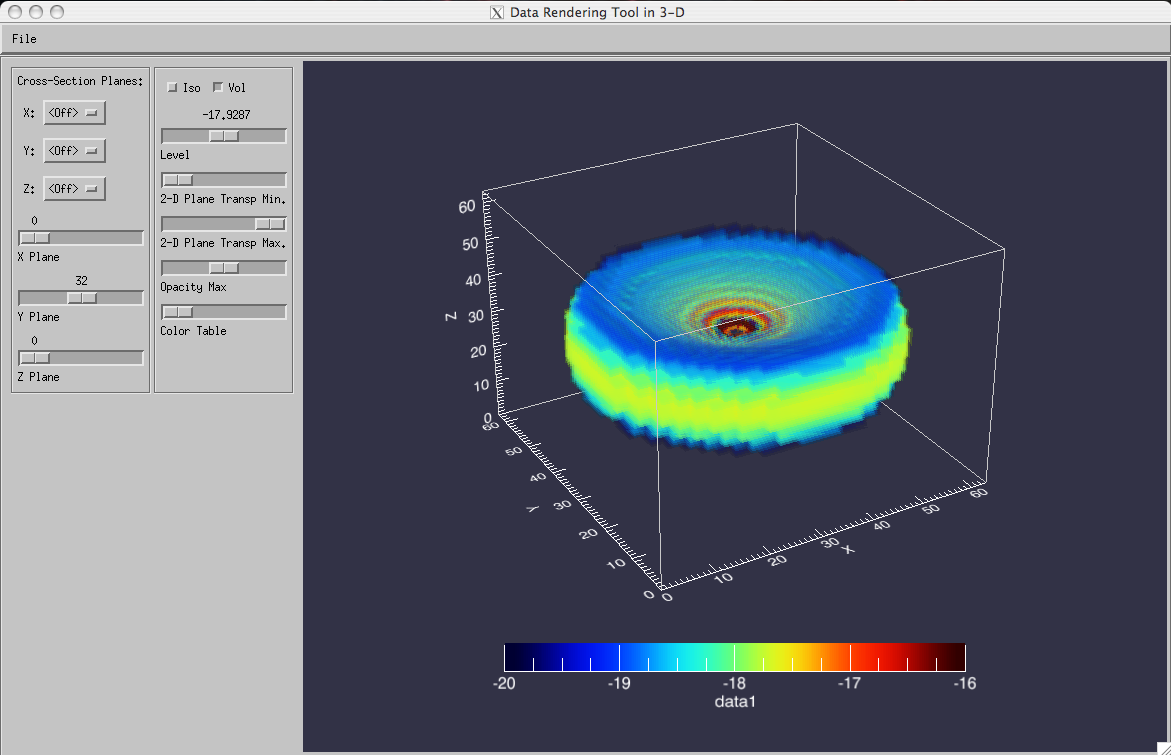
\includegraphics[width=0.9\textwidth]{render3d.eps}}
\caption{\label{fig-render3d} The graphical user interface (GUI) {\small\tt
    render3d.pro} that allows you to analyze 3-D regularly spaced
  datacubes. In Chapter \ref{chap-radmc3d-internal-analysis-tools} it is
  described how to create regularly spaced datacubes of any variable in the
  model from a complex AMR-based model. Shown in this figure is in fact
  the {\small\tt run\_disk\_1/} model, which is an AMR-based model, in which
  the trick of Chapter \ref{chap-radmc3d-internal-analysis-tools} is applied
  to create a regularly spaced box.}
\end{figure}
Note: Apart from all the sliders and buttons, try also out how you can
interactively rotate the 3-D datacube with the mouse: just click on the
plotting window and drag while keeping clicked.



%----------------------------------------------------------------------------
%               CHAPTER: USING THE IDL TOOL SET
%----------------------------------------------------------------------------
\chapter{Model analysis (II): Tools inside of radmc3d}
\label{chap-radmc3d-internal-analysis-tools}
There are also some special purpose features in the Fortran-90 {\small\tt
  radmc3d} code that can be useful for analyzing complex AMR-gridded models.

\section{Making a regularly-spaced datacube (`subbox') of AMR-based models}
\label{sec-subbox}
Because handling AMR-based models in IDL or other data analysis packages can
be rather cumbersome, we decided that it would be useful to create the
possibility in {\small\tt radmc3d} to generate 1-D, 2-D or 3-D regularly
spaced `cut-outs' or `sub-boxes' (whatever you want to call them) of any
variable of the model. An example of how this all works, and how these 1-D,
2-D or 3-D sub-boxes can be used with the {\small\tt render3d.pro} tool set
described in Section \ref{sec-render3d}, is given in the model {\small\tt
  examples/run\_disk\_1/}.

\subsection{Creating and reading a subbox from within IDL}
If all the IDL tools are set up properly, you can make use of this datacube
creation feature of {\small\tt radmc3d} entirely through IDL. An example, 
type in IDL:
\begin{asciibox}\begin{verbatim}
.r readradmc.pro
q=subbox('dust_density')
\end{verbatim}\end{asciibox}
This creates a box with the size of the original model box, but this time
regularly spaced. The data is in {\small\tt q.data}. You can see this by 
typing:
\begin{asciibox}\begin{verbatim}
help,q,/str
\end{verbatim}\end{asciibox}
You will see that {\small\tt q.data} is a 3-D array of 64x64x64 (default
size). 

The box contains the dust density. You can specify the
size and the number of grid points of the regularly-spaced box:
\begin{asciibox}\begin{verbatim}
.r readradmc.pro
@natconst.pro
q=subbox('dust_density',nxyz=64,size=2*100*AU)
.r render3d.pro
render3d,alog10(q.data>1d-20)
\end{verbatim}\end{asciibox}
NOTE: The {\small\tt size} keyword is the {\em full-width} size of the box!
So if you want to capture a disk with radius 100 AU, then you must have a
box size of 200 AU.

You can also make and read in separate steps:
\begin{asciibox}\begin{verbatim}
.r readradmc.pro
@natconst.pro
makesubbox,'dust_density',nxyz=64,size=200*AU
q=readsubbox('dust_density_subbox.out')
.r render3d.pro
render3d,alog10(q.data>1d-20)
\end{verbatim}\end{asciibox}
You can specify the box location with the keyword {\small\tt pos}:
\begin{asciibox}\begin{verbatim}
q=subbox('dust_density',nxyz=64,size=200*AU,pos=[30,30,30]*AU)
\end{verbatim}\end{asciibox}
or by specifying the corners of the box directly:
\begin{asciibox}\begin{verbatim}
q=subbox('dust_density',nxyz=64,box=[-1,1,-1,1,-1,1]*80*AU)
\end{verbatim}\end{asciibox}

Note that if you have {\small\tt radmc3d} already running in the background
using the {\small\tt child} mode (see Chapter \ref{chap-child-mode}) then
you can do the above commands more quickly by directly communicating through
the pipe by passing the keyword {\small\tt iounit=<myiounitnumber>} (where
the thing in between $<$ and $>$ should be the unit number of the biway pipe
to {\small\tt radmc3d}) to the above routines {\small\tt makesubbox} or
{\small\tt subbox}.

Currently available quantities you can write out as a subbox are:
\begin{itemize}
\item {\em Dust density:} Give {\small\tt 'dust\_density'} as first argument to
the subbox command.
\item {\em Dust temperature:} Give {\small\tt 'dust\_temperature'} as first argument to
the subbox command.
\item {\em Molecular/atomic level populations:} Give {\small\tt 'levelpop'}
  as first argument to the subbox command. Note that it will write out a subbox
  file for each molecule separately. For instance, for CO it would produce
  a file called {\small\tt 'levelpop\_co\_subbox.out'}. Each of these files can
  be read with the {\small\tt readsubbox} command (see above).
\end{itemize}

\subsection{Creating and reading a subbox by directly communicating with radmc3d}
You can also call {\small\tt radmc3d} directly from the shell asking it to make
the subbox. Here is an example:
\begin{asciibox}\begin{verbatim}
./radmc3d subbox_dust_temperature subbox_nxyz 64 64 64 \
subbox_xyz01 -2.d15 2.d15 -2.d15 2.d15 -2.d15 2.d15
\end{verbatim}\end{asciibox}
An example for the level populations would be:
\begin{asciibox}\begin{verbatim}
./radmc3d subbox_levelpop subbox_nxyz 64 64 64 \
subbox_xyz01 -2.d15 2.d15 -2.d15 2.d15 -2.d15 2.d15
\end{verbatim}\end{asciibox}

{\em Note about subbox for level populations:} By default all level populations
will be written out. However, if you would add the {\small\tt subbox\_levelpop}
keyword in a call to RADMC-3D for making an image or spectrum, then it will
only write out the level populations that have been used for that image. Example:
\begin{asciibox}\begin{verbatim}
./radmc3d image lambda 2600 subbox_levelpop subbox_nxyz 64 64 64 \
subbox_xyz01 -2.d15 2.d15 -2.d15 2.d15 -2.d15 2.d15
\end{verbatim}\end{asciibox}
would give a much smaller {\small\tt 'levelpop\_co\_subbox.out'} file, because
only the first two levels are included (remember that $\lambda=2600\,\mu$m is the
J1-0 line of CO). See Section \ref{sec-calcstore-levpop} for more information on
how RADMC-3D automatically selects a subset of levels for storage in the global
array (and thus also for writing out to file). 

\subsection{Format of the subbox output files}
All the files produced by the subbox method have the following format:
\begin{asciibox}\begin{verbatim}
iformat                                  <=== Typically 2 at present
nx ny nz nv                              <=== Box of nx*ny*nz cells, each with nv values
x0 x1 y0 y1 z0 z1                        <=== The x, y and z boundaries of the box
phi1 theta phi2                          <=== Three rotation angles of the box
                                         <=== Empty line 
1 2 3 4 ....                             <=== Identifications of the nv values 
                                         <=== Empty line 
data[ix=1,iy=1,iz=1,iv=1]
data[ix=2,iy=1,iz=1,iv=1]
.
.
data[ix=nx,iy=1,iz=1,iv=1]
data[ix=1,iy=2,iz=1,iv=1]
.
.
.
data[ix=nx,iy=ny,iz=nz,iv=1]
                                         <=== Empty line between components
data[ix=1,iy=1,iz=1,iv=2]
.
.
data[ix=nx,iy=ny,iz=nz,iv=2]
                                         <=== Empty line between components
.
.
.
                                         <=== Empty line between components
data[ix=1,iy=1,iz=1,iv=nv]
.
.
data[ix=nx,iy=ny,iz=nz,iv=nv]
\end{verbatim}\end{asciibox}
and they are always in ascii format. For a subbox of the level populations the
identification numbers are the levels. For instance, if only the populations of
levels 4 and 8 are in this file, then {\small\tt nv=2} and the line with
the identification numbers will be {\small\tt 4 8}. For all other quantities
(dust density, dust temperature) this line of identification numbers is simply
{\small\tt 1 2 3} etc.


\section{Alternative to subbox: arbitrary sampling of AMR-based models}
\label{sec-sampling}
%
For some purposes it is useful to sample values of various quantities at
arbitrary positions in the grid. The idea is very much like the subbox
method of Section \ref{sec-subbox}, but instead of a regular subbox grid
the user provides a list of 3-D points where he/she wants to sample the
variables of the model. Here is how to do this. First you must produce
a file containing the list of 3-D positions. The file is called
{\small\tt sample\_points.inp} and is an ascii file that looks as
follows:
\begin{asciibox}\begin{verbatim}
iformat                                  <=== Typically 1 at present
npt                                      <=== Nr of 3-D sampling points
xpt[1]  ypt[1]  zpt[1]                   <=== 3-D coordinates of point 1
xpt[2]  ypt[2]  zpt[2]                   <=== 3-D coordinates of point 2
xpt[3]  ypt[3]  zpt[3]                   <=== 3-D coordinates of point 3
...
...
\end{verbatim}\end{asciibox}
An example for the case in which you want to sample at just one point:
\begin{asciibox}\begin{verbatim}
1
1
1.49d13   4.02d14   1.03d12
\end{verbatim}\end{asciibox}
If you want to let RADMC-3D do the sampling of the dust density and
temperature, type (after you have calculated the temperature using
{\small\tt radmc3d mctherm}):
\begin{asciibox}\begin{verbatim}
radmc3d sample-dustdens sample-dusttemp
\end{verbatim}\end{asciibox}
You can also do the dust temperature calculation and the sampling in one
go:
\begin{asciibox}\begin{verbatim}
radmc3d mctherm sample-dustdens sample-dusttemp
\end{verbatim}\end{asciibox}
You can also do only {\small\tt sample-dusttemp} or only {\small\tt
  sample-dustdens}. The output is written to files {\small\tt
  dust\_density\_sample.out} resp.\ {\small\tt
  dust\_temperature\_sample.out}. The format of these files is (take
dust density as example):
\begin{asciibox}\begin{verbatim}
iformat                                  <=== Typically 2 at present
npt  nv                                  <=== Nr of point and size of datavector
                                         <=== Empty line
1 2 3 4 ....                             <=== Identifications of the nv values 
                                         <=== Empty line
dustdensity[ipt=1,iv=1]
dustdensity[ipt=2,iv=1]
...
dustdensity[ipt=npt,iv=1]
                                         <=== Empty line between components
dustdensity[ipt=1,iv=2]
...
dustdensity[ipt=npt,iv=2]
                                         <=== Empty line between components
...
                                         <=== Empty line between components
dustdensity[ipt=npt,iv=nv]
\end{verbatim}\end{asciibox}
where {\small\tt nv} is in this case the nr of species of dust and 
{\small\tt iv}={\small\tt ispecies}.

For a sample of the level populations the identification numbers are the
levels. For instance, if only the populations of levels 4 and 8 are in this
file, then {\small\tt nv=2} and the line with the identification numbers
will be {\small\tt 4 8}. For all other quantities (dust density, dust
temperature) this line of identification numbers is simply {\small\tt 1 2 3}
etc.

Later we will add other possible arrays to sample (at the moment it is only
dust density, dust temperature and level populations). But you can also
implement this yourself. Search in the following files for the following
parts to add your own sampling:
\begin{itemize}
\item In {\small\tt rtglobal\_module.f90}: Search for {\small\tt 
do\_sample\_dustdens} and add your own variable, e.g.\ {\small\tt
do\_sample\_myvariable}.
\item In {\small\tt main.f90}: Search for {\small\tt do\_sample\_dustdens}
  and you will find all places where you have to add your own stuff, i.e.\
  where you will have to add statements like {\small\tt
    if(do\_sample\_myvariable)} or where you have to set {\small\tt
    do\_sample\_myvariable=.true.} or reset {\small\tt
    do\_sample\_myvariable=.false.} etc. 
\end{itemize}
That should do it.

%----------------------------------------------------------------------------
%            CHAPTER: USING VTK-COMPIANT VISUALIZATION TOOLS
%----------------------------------------------------------------------------
\chapter{Model analysis (III): Visualization with VTK tools (e.g. Paraview or VisIt)}
\label{chap-vtk-output}
%
Since 3-D models can be very hard to visualize, and since RADMC-3D is not
made for quick rendering, it can be very useful to make use of a number of
freely available 3-D rendering tools, for example:
\begin{itemize}
\item Paraview ({\small\tt www.paraview.org})
\item VisIt ({\small\tt visit.llnl.gov})
\end{itemize}
RADMC-3D can create data files for use with these tools. The file format is
VTK (Visual Tool Kit), which is a simple ascii file format which is used by
various programs. Those tools are not only useful for visualizing the
3-D structure of the model, but also for visualizing the structure of the
grid which can be, when using AMR, rather complex. 

The file that RADMC-3D writes is called {\small\tt model.vtk}. You should be
able to open it directly from within e.g.\ paraview. Figure
\ref{fig-disk-with-vtk} gives an example of how you can analyze a complex
geometry with AMR refinement with Paraview. The file {\em always} includes
the information about the grid. In addition you can also make RADMC-3D add
scalar fields or vector fields.

To create a VTK file for viewing the grid only, type:
\begin{asciibox}\begin{verbatim}
radmc3d vtk_grid
\end{verbatim}\end{asciibox}
To create a VTK file for viewing the gas density (this file then also
includes the grid of course) type:
\begin{asciibox}\begin{verbatim}
radmc3d vtk_gas_density
\end{verbatim}\end{asciibox}
Since density can span a huge range, the 10-log of the density (in units of
gram/cm$^3$) is written instead. For the gas temperature:
\begin{asciibox}\begin{verbatim}
radmc3d vtk_gas_temperature
\end{verbatim}\end{asciibox}
which is written in Kelvin (and linearly, not log). For the dust density of
dust species 1:
\begin{asciibox}\begin{verbatim}
radmc3d vtk_dust_density 1
\end{verbatim}\end{asciibox}
and for dust species 2:
\begin{asciibox}\begin{verbatim}
radmc3d vtk_dust_density 2
\end{verbatim}\end{asciibox}
Also these densities are 10-log. RADMC-3D typically computes the dust
temperature using a Monte Carlo approach. By typing
\begin{asciibox}\begin{verbatim}
radmc3d vtk_dust_temperature 1
\end{verbatim}\end{asciibox}
RADMC-3D will try to read the dust temperature from the file
{\small\tt dust\_temperature.dat} (if this file has been created 
earlier by a {\small\tt radmc3d mctherm} call) and then create
the VTK file. You can also let RADMC-3D compute the temperature
directly and write it out to VTK right afterward:
\begin{asciibox}\begin{verbatim}
radmc3d mctherm vtk_dust_temperature 1
\end{verbatim}\end{asciibox}

If you are doing line transfer you may wish to visualize the number density
of the molecules (or atoms):
\begin{asciibox}\begin{verbatim}
radmc3d vtk_molspec 1
\end{verbatim}\end{asciibox}
(for molecular species 1). This number density (in cm$^{-3}$) is also
written in 10-log form.  You may also wish to visualize the polulations of
level 1 (ground state) of molecule 2:
\begin{asciibox}\begin{verbatim}
radmc3d vtk_levelpop 2 1
\end{verbatim}\end{asciibox}
The gas velocity field can be written to VTK file by
\begin{asciibox}\begin{verbatim}
radmc3d vtk_velocity
\end{verbatim}\end{asciibox}
This is a vector field.

Note: The VTK mode works for 3-D cartesian and 3-D spherical coordinates
(thanks, Attila Juhasz, for the 3-D spherical mode!).


%
\begin{figure}
\centerline{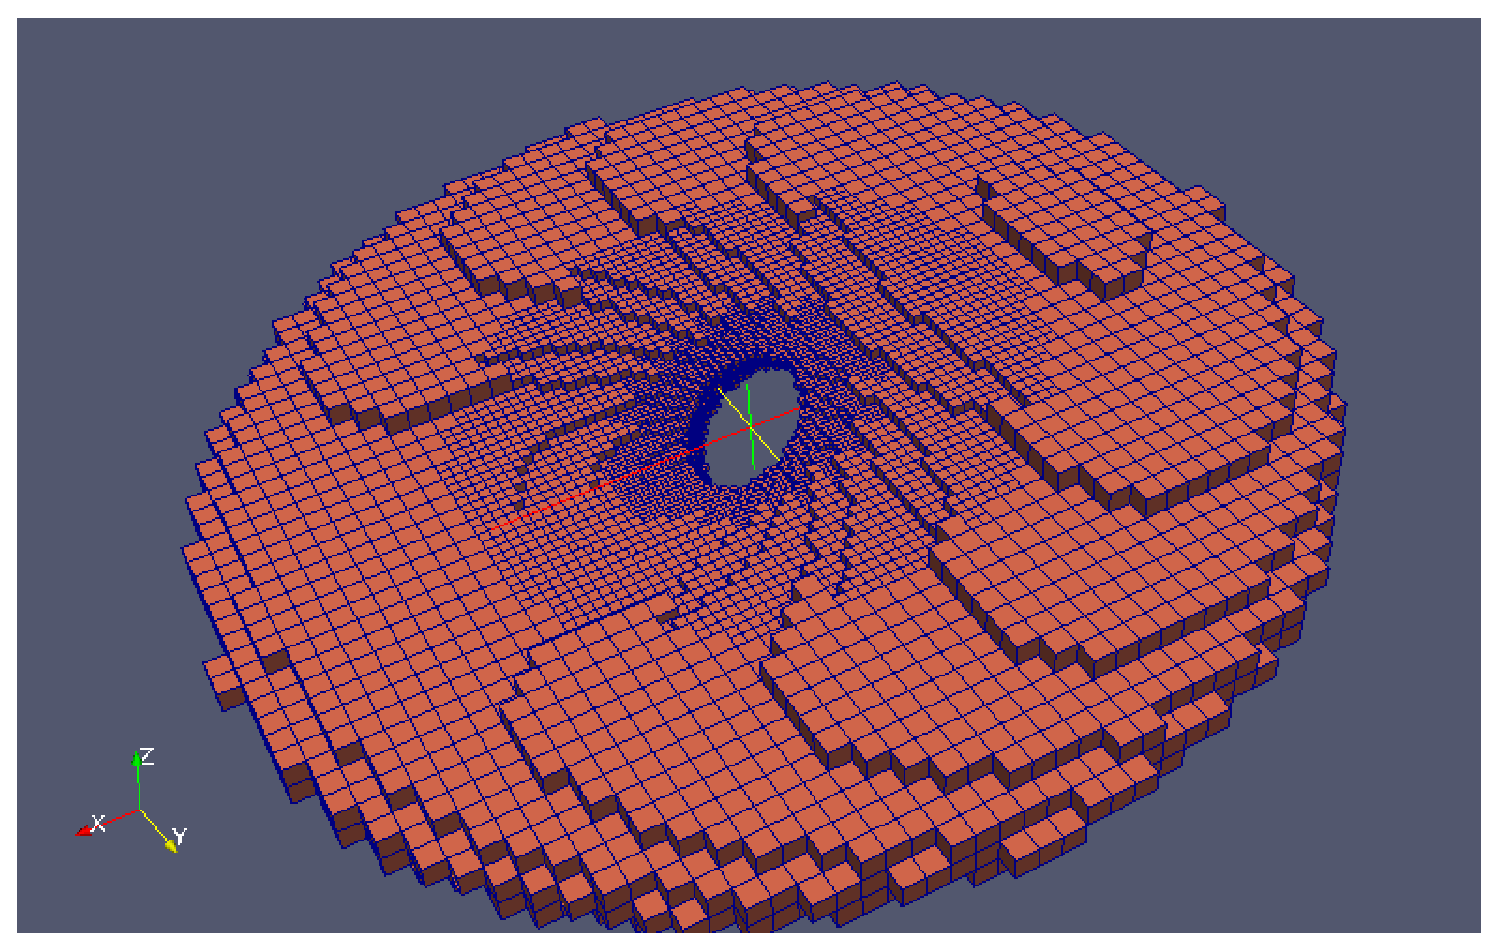
\includegraphics[width=0.7\textwidth]{disk_rosenfeld.eps}}
\caption{\label{fig-disk-with-vtk}
Example of image created with Paraview, using the VTK output of RADMC-3D.
The model shown here is a warped disk model by Katherine Rosenfeld, 
in 3-D cartesian coordinates with oct-tree AMR refinement.
}
\end{figure}
%

%
\begin{figure}
\centerline{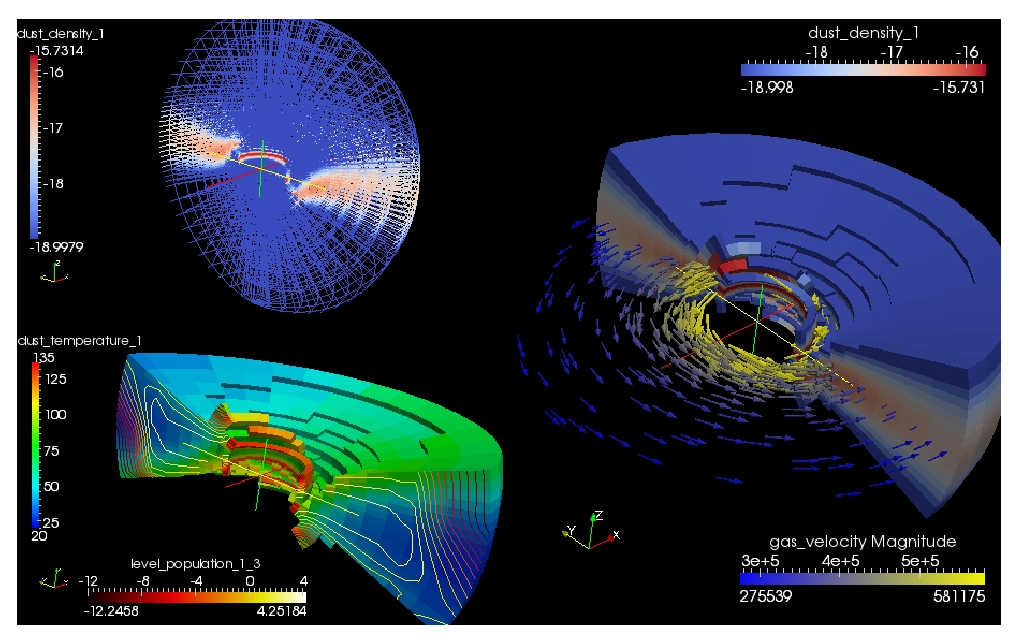
\includegraphics[width=0.85\textwidth]{model_juhasz_vtk_lowres.eps}}
\caption{\label{fig-modeljuhasz-with-vtk}
Example of image created with Paraview, using the VTK output of RADMC-3D.
The model shown here is a warped disk model by Attila Juhasz, in 3-D
spherical coordinates with separable refinement, but without AMR refinement.
The model is kept low-resolution on purpose, to show the grid structure
better.
}
\end{figure}
%


%----------------------------------------------------------------------------
%                   CHAPTER: A DISK MODELING SETUP GUI
%----------------------------------------------------------------------------
\chapter{Creating Protoplanetary Disk Models using a GUI}
\label{chap-gui-ppdisk}
%
\centerline{{\Large\em Author: A.~Juhasz}}\vspace{1em}
%
Attila Juhasz has created an IDL-driven graphical user interface (GUI) for
modeling protoplanetary disks. The GUI for RADMC-3D was developed for YSO
disks/envelopes but can also be used (to some extent) as a general purpose
user interface. Or it may serve as a template for other users to create GUIs
for their own models. The GUI is written in IDL and consits of five IDL
routines; radmc3d$\_$gui.pro, read$\_$params$\_$radmc3d.pro,
problem$\_$params.pro, problem$\_$setup$\_$yso.pro,
my$\_$gap$\_$function.pro.

\begin{itemize}
\item {\bf radmc3d$\_$gui.pro} This file contains all the widget definitions and basically everything related
to the visualization. 
\item {\bf read$\_$params$\_$radmc3d.pro} This file contains two functions to read and write the parameters
into a file. 
\item {\bf problem$\_$params.pro} Those, who have actually worked with the 2D version of RADMC, this file
should look familiar. This file contains all parameters required to set up the problem and create the input
files for RADMC 3D. 
\item {\bf problem$\_$setup.pro} This file has also the same function as in the 2D version of RADMC. On
the basis of the parameters stored in problem$\_$params.pro, it creates the input files to RADMC 3D. 
\item {\bf my$\_$gap$\_$function.pro} This is a small routine to cut a gap in the disk to demonstrate, how
one can use this GUI with one's own dust density setup. 
\item {\bf my$\_$gap2$\_$function.pro} This is a small routine to cut a second gap in the disk 
(in the exact same way as my$\_$gap$\_$function.pro) to demonstrate, how
one can use this GUI with one's own dust density setup. 
\end{itemize}

\section{How to run the GUI}
The GUI can be run in a very simple way. First an IDL should be started and 
the radmc3d$\_$gui.pro routine should be compiled.
\begin{verbatim}
IDL> .r radmc3d_gui
\end{verbatim}
With this step not only radmc3d$\_$gui.pro, but also all other necessary
files/routines will be compiled (Note: it assumes that you are in the
examples/run$\_$whatever directory and the readradmc.pro file is located in
the ../../idl/ directory). After the compilation the GUI is ready to be run
with the command radmc3d$\_$gui:
\begin{verbatim}
IDL> radmc3d_gui
\end{verbatim}
After this command has been executed the user should see a window similar to
that in Fig\,\ref{fig-gui-ppdisk}.
%
\begin{figure}
\centerline{\includegraphics[angle=90,width=0.9\textwidth]{gui_ppdisk.eps}}
\caption{\label{fig-gui-ppdisk} The graphical user interface for a
  protoplanetary disk model. Author: A.~Juhasz.}
\end{figure}
%

To make things easy (especially for those ones who use a radiative transfer
code for the first time) the GUI comes with a simple 'default' setup for the
dust density distribution. This setup is based on a common parametrization
of a protoplanetary disk and a surrounding envelope. However, the user may
want to change the whole density distribution or may want to add
extension(s) to this setup (e.g. a gap in the disk). One can add his/her own
extension(s) to the model setup so, that the GUI will recognize them and new
tabs will automatically open to access the parameters of these extensions.


\section{Create your own setup and/or open your own tab}
Adding new extension to the code which appears as a new tab in the dust
density setup frame is relatively easy, one only needs to keep a few
rules. To make it clear how this can be done it is useful to understand what
the GUI does behind the buttons and windows. In a few steps the GUI does the
following;

\begin{enumerate}
\item Write the parameter values to problem$\_$params.pro
\item Run problem$\_$setup$\_$yso.pro to create all necessary input files for RADMC3D
\item Run RADMC3D mctherm to calculate the temperature structure
\item Run RADMC3D to calculate images/spectra
\end{enumerate}

After Step\,2. any arbitrary IDL procedure can be run to modify (or even
completely re-create) the dust density distribution. Such a procedure can be
integrated to the GUI in the following way;

\begin{itemize}
\item The procedure should not accept any keywords or input variable,
  instead, the user should add the @problem$\_$params.pro line after the
  procedure name, allowing the procedure to access the variables in
  problem$\_$params.pro;
\begin{verbatim}
pro my_arbitrary_procedure
@problem_params.pro
\end{verbatim}
\item Create a new section of parameters in problem$\_$params.pro which will
  be used in the user's procedure.  For examle;
\begin{verbatim}
;
; My extra function - example 
;   Cut a gap in the disk reducing the density by an arbitrary factor
;
extra_gap_tab_name = 'My gap function' ; Name of the tab in the GUI
extra_gap_enable = 1                   ; 0-Enable, 1-Disable this function
extra_gap_func = 'my_gap_function'     ; Name of the user defined function 
extra_gap_rin = 5.0*AU                 ; Inner radius of the gap
extra_gap_rout = 10.*AU                ; Outer radius of the gap
extra_gap_drfact = 1d-4                ; Density reduction factor in the gap

\end{verbatim}
\item The parameter names should look like; extra$\_$secname$\_$pname. The
  'extra' means that this is an additional parameter for which a new tab
  should be opened. The 'secname' will be the identifier of this section of
  parameters within the widgets and should be the same for all parameters
  within this section. The 'pname' is the actual parameter name, that can be
  any arbitrary name.
\item Each new section should contain a parameter called
  'extra$\_$secname$\_$tab$\_$name', which will be the title of the new tab
  which will open in the dust density setup frame.
\item Each new section should contain a parameter called
  'extra$\_$secname$\_$func', which should be the name of the user's
  procedure.
\item Each new section should contain a parameter called
  'extra$\_$secname$\_$enable', which should have a value of 0 or 1 and
  disables or enables the execution of the user's procedure after
  problem$\_$setup$\_$yso.pro.
\end{itemize}

If the user followed the instructions above and start the GUI a new tab in
the density setup frame should open for the user's procedure. Input fields
for the parameters will have the parameter names as titles. If one made
comments in problem$\_$params.pro at the end of a line to explain the
meaning of the parameter at the beginning of the line, this
explanation/comment will be available in the Help menu under "Help on
parameters".  Two examples were given in the current problem$\_$params.pro
to open gaps in the dust density distribution.
 



%----------------------------------------------------------------------------
%                CHAPTER: PORTING MODELS FROM OLD RADMC
%----------------------------------------------------------------------------
\chapter{How to convert old-style RADMC models to RADMC-3D}
\label{chap-porting-from-radmc}
%
Some users of RADMC-3D may have used the predecessor program RADMC before.
The input files of RADMC are different from those used by RADMC-3D. You may
have model setups created for RADMC which you would like to feed into
RADMC-3D. The best way would be of course to edit your {\small\tt
  problem\_***.pro} files and make sure that they create the RADMC-3D
input files instead of the RADMC input files. But that costs quite some
work, and you may make errors.

We offer the IDL routine {\small\tt radmc2radmc3d.pro} in the {\small\tt
  idl/} directory that automatically converts all the RADMC input files
into RADMC-3D input files. In particular, it will do the following
conversion:\vspace{1em}\\
\centerline{\begin{tabular}{|l|l|}
\hline
RADMC & RADMC-3D \\
\hline
{\small\tt radius.inp} \& {\small\tt theta.inp} & {\small\tt amr\_grid.inp}\\
{\small\tt starinfo.inp} \& {\small\tt starspectrum.inp} & {\small\tt stars.inp}\\
{\small\tt dustdens.inp}  & {\small\tt dust\_density.inp}\\
-  & {\small\tt radmc3d.inp}\\
\hline
\end{tabular}}\vspace{1em}\\
The file {\small\tt radmc.inp} is ignored for now, and instead a fresh
{\small\tt radmc3d.inp} is created. While RADMC-3D would read {\small\tt
  radmc.inp} if no {\small\tt radmc3d.inp} is present, the presence of
{\small\tt radmc3d.inp} means that RADMC-3D will read {\small\tt radmc3d.inp}
(and {\em not} read {\small\tt radmc.inp}).

The opacity files are kept as they are. While the recommended style for
the opacities is the {\small\tt dustkappa\_*.inp} file, RADMC-3D
can also read the old style {\small\tt dustopac\_*.inp} files. Also
the {\small\tt frequency.inp} file is kept as it is.

NOTE: For now the quantum-heated grains are not ported to RADMC-3D. Also
some specialties of the RADMC code may not yet work in RADMC-3D -- just 
keep this in mind.

So if you have a working model for RADMC, and you want to run it with
RADMC-3D, then just go into the model directory, go into IDL and type:
{\small\begin{verbatim}
.r radmc2radmc3d.pro
\end{verbatim}}
and this should convert the files from RADMC-style to RADMC-3D-style,
as described above. Note that you must now redo the thermal Monte Carlo,
because RADMC-3D reads its own style of dust temperature file. So go
out of IDL and type (on the shell):
{\small\begin{verbatim}
radmc3d mctherm
\end{verbatim}}
wait until it is finished, and now you can make your spectra and images.





%----------------------------------------------------------------------------
%                       CHAPTER: PROBLEM HUNTING
%----------------------------------------------------------------------------
\chapter{Tips, tricks and problem hunting}
\label{chap-problem-hunting}
%
\section{Tips and tricks}
%
{\small\tt RADMC-3D} is a large software package, and the user will in all
likelihood not understand all its internal workings. In this section we will
discuss some issues that might be useful to know when you do modeling.
\begin{itemize}
\item {\em Things that can drastically slow down ray-tracing:}\\
  When you create images or spectra, {\small\tt radmc3d} will perform a
  ray-tracing calculation. You may notice that sometimes this can be very
  fast, but for other problems it can be very slow. This is because,
  depending on which physics is switched on, different ray-tracing
  strategies must be followed. For instance, if you use a dust opacity
  without scattering opacity (or if you switch dust scattering off by
  setting {\small\tt scattering\_mode\_max} to 0 in the {\small\tt
    radmc3d.inp} file), and you make dust continuum images, or make SEDs, this
  may go very rapidly: less than a minute on a modern computer for grids of
  256x256x256. However, when you include scattering, it may go slower. Why
  is that? That is because at each wavelength {\small\tt radmc3d} will now
  have to make a quick Monte Carlo scattering model to compute the dust
  scattering source function. This costs time. And it will cost more time if
  you have {\small\tt nphot\_scat} set to a high value in the {\small\tt
    radmc3d.inp} file, although it will create better images. Furthermore, if
  you {\em also} include gas lines using the simple LTE or simple LVG
  methods, then things become even slower, because each wavelength channel
  image is done after each other, and each time all the populations of the
  molecular levels have to be re-computed. If dust scattering would be
  switched off (which is for some wavelength domains presumably not a bad
  approximation; in particular for the millimeter domain), then no
  scattering Monte Carlo runs have to be done for each wavelength. Then the
  code can ray-trace all wavelength simultaneously: each ray is traced only
  once, for all wavelength simultaneously. Then the LTE/LVG level
  populations have to be computed only once at each location along the ray.
  So if you use dust and lines simultaneously, it can be advantageous for
  speed if you can afford to switch off the dust scattering, for instance,
  if you model sub-millimeter lines in regions with dust grains smaller than
  10 micron or so. If you must include scattering, but your model is not so
  big that you may get memory limitation problems, then you may also try the
  fast LTE or fast LVG modes: in those modes the level populations are
  pre-computed before the ray-tracing starts, which saves time. But that may
  require much memory.
\end{itemize}


\section{Bug hunting}
Although we of course hope that {\small\tt radmc3d} will not run into
troubles or crash, it is nevertheless possible that it will. There are
several ways by which one can hunt for bugs, and we list here a few 
obvious ones:
\begin{itemize}
\item In principle the {\small\tt Makefile} should make sure that all
dependencies of all modules are correct, so that the most dependent
modules are compiled last. But during the further development of the
code perhaps this may be not 100\% guaranteed. So try do {\small\tt 
make clean} followed by {\small\tt make} (or {\small\tt make install})
to assure a clean make.
\item In the {\small\tt Makefile} you can add (or uncomment) the line \\
{\small\tt BCHECK   = -fbounds-check}, if you use {\small\tt gfortran}.
Find the array boundary check switch on your own compiler if it is 
not {\small\tt gfortran}.
\item Make sure that in the {\small\tt main.f90} code the variable
{\small\tt debug\_check\_all} is set to 1. This will do some on-the-fly
checks in the code.
\end{itemize}


\section{Some tips for avoiding troubles and for making good models}
Here is a set of tips that we recommend you to follow, in order to avoid
troubles with the code and to make sure that the models you make are OK.
This list is far from complete! It will be updated as we continue to
develop the code.
\begin{enumerate}
\item Make a separate directory for each model. This avoids confusion with
  the many input and output files from the models.
\item When experimenting: regularly keep models that work, and continue
  experimenting with a fresh model directory. If things go wrong later, you
  can always fall back on an older model that {\em did} work well.
\item Keep model directories within a parent directory of the code, just
  like it is currently organized. This ensures that each model is always
  associated to the version of the code for which it was developed.  If you
  update to a new version of the code, it is recommended to simply copy the
  models you want to continue with to the new code directory (and edit the
  {\small\tt SRC} variable in the {\small\tt Makefile} if you use the
  techniques described in Section \ref{sec-special-purpose-compile} and
  Chapter \ref{chap-internal-setup}).
\item If you make a new model, try to start with as clean a directory as
  possible. This avoids that you accidently have a old files hanging around,
  their presence of which may cause troubles in your new model.  So if you
  make a model update, make a new directory and then copy only the files
  that are necesary (for instance, {\small\tt problem\_setup.pro},
  {\small\tt dustkappa\_silicate.inp}, {\small\tt Makefile} and other
  necessary files). One way of doing this easily is to write a little perl
  script or csh script that does this for you.
\item In the example model directories there is always a {\small\tt Makefile}
  present, even if no local {\small\tt *.f90} files are present. The idea
  is that by typing {\small make cleanall} you can safely clean up the 
  model directory and restore it to pre-model status. This can be useful 
  for safely cleaning model directories so that only the model setup files
  remain there. It may save enormous amounts of disk space. But of course,
  it means that if you revisit the model later, you would need to redo
  the Monte Carlo simulations again, for instance. It is a matter of 
  choice between speed of access to results on the one hand and disk space
  on the other hand.
\item If you use LVG or escape probability to compute the level populations
  of molecules, please be aware that you must include all levels that could
  be populated, not only the levels belonging to the line you are interested
  in. 
\end{enumerate}


\section{Careful: Things that might go wrong}
\label{sec-things-going-wrong}
%
In principle RADMC-3D should be fine-tuned such that it produced reliable
results in most circumstances. But radiative transfer modeling, like all
kinds of modeling, is not an entirely trivial issue. Extreme circumstances 
can lead to wrong results, if the user is not careful in doing various
sanity checks. This section gives some tips that you, the user, may wish
to do to check that the results are ok. This is not an exhaustive list!
So please remain creative yourself in coming up with good tests and checks.
\begin{enumerate}
\item {\bf Too low number of photon packages for thermal Monte Carlo}\\
  If the number of photon packages for the thermal Monte Carlo simulation
  (Section \ref{sec-dust-thermal-monte-carlo}) is too low, the dust
  temperatures are going to be very noisy. Some cells may even have
  temperature zero. This may not only lead to noisy images and spectra,
  but also simply wrong results. However, deep inside optically thick
  clouds (or protoplanetary disks) it will be hard to avoid this problem.
  Since those regions are very deep below the $\tau=1$ surface, it might
  not be always too critical in that case. A bit of experimenting might
  be necessary.
\item {\bf Too low number of photon packages for scattering}\\
  When making images or spectra in which dust scattering is important, the
  scattered light emissivity is computed by a quick Monte Carlo simulation
  before the ray-tracing (see Section \ref{sec-scat-monte-carlo}). This
  requires the setting of the number of photon packages used for this (the
  variable {\small\tt nphot\_scat} for images and equivalently {\small\tt
    nphot\_spec} for spectra, both can be set in the {\small\tt radmc3d.inp}
  file). If you see too much ``noise'' in your scattering image, you can
  improve this by setting {\small\tt nphot\_scat} to a larger value (default
  = 100000). If your spectrum contains too much noise, try setting
  {\small\tt nphot\_spec} to a larger value (default = 10000).
\item {\bf Too optically thick cells at the surface or inner edge}\\
  You may want to experiment with grid resolution and refinement. Strictly
  speaking the transition from optically thin to optically thick, as seen
  both by the radiation entering the object and by the observer, has to
  occur over more than one cell. That is for very optically thick models,
  one may need to introduce grid refinement in various regions. As an
  example: an optically thick protoplanetary disk may have an extremely
  sharp thin-thick transition near the inner edge. To get the spectra and
  images right, it is important that these regions are resolved by the grid
  (note: once well inside the optically thick interior, it is no longer
  necessary to resolve individual optical mean free paths, thankfully). It
  should be said that in practice it is often impossible to do this in full
  strictness. But you may want to at least experiment a bit with refining
  the grid (using either ``separable refinement'', see Section
  \ref{sec-separable-refinement}, or AMR refinement, see Section
  \ref{sec-amr-grid-oct-tree}). An example how wrong things can go at the
  inner edge of a protoplanetary disk, if the inner cells are not assured to
  be optically thin through grid refinement (and possibly additionally a bit
  of smoothing of the density profile too) is given in
  Fig.~\ref{fig-innerrim-lowres}.
  % 
  \begin{figure}
    \centerline{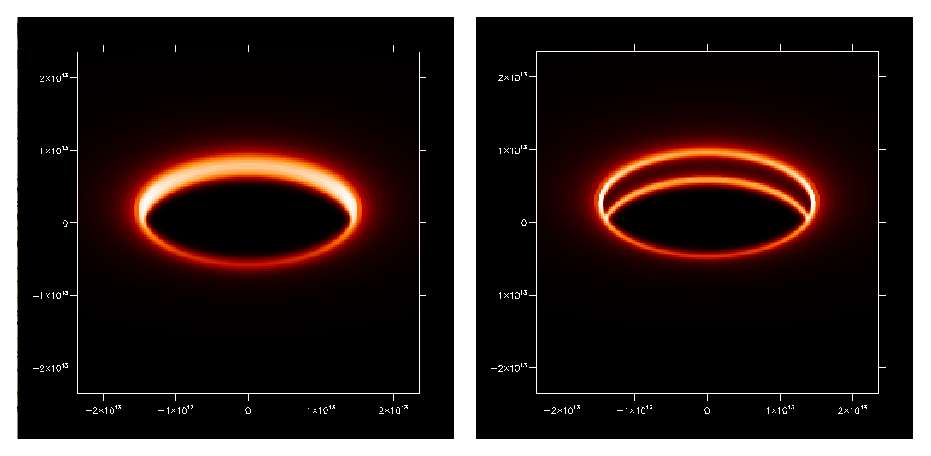
\includegraphics[width=0.5\textwidth]{XFIG/innerrim.eps}}
    \caption{\label{fig-innerrim-lowres}Example of what can go wrong with
      radiative transfer if the inner cells of a model are optically thick
      (i.e.\ if no grid refinement is used, see Section
      \ref{sec-separable-refinement}). Shown here are scattered light images
      at $\lambda=0.7\mu$m wavelength of the inner rim of a protoplanetary
      disk, but with the star removed with an ideal choronograph. The color
      scale is linear. The radial grid is taken to be logarithmically spaced
      with $\Delta R/R=0.04$.  Left image: the inner cells are marginally
      optically thin $\Delta\tau\simeq 1$, creating a bright inner ring, as
      is expected. Right image: ten times higher optical depth, making the
      inner cells optically thick with roughly $\Delta\tau\simeq 10$,
      resulting in a wrong image in which the emission near the midplane is
      strongly reduced.  The reason for that is that the scattering source
      function, due to photons scattering at the inner 10\% of the inner
      cell, is diluted over the entire cell, making the scattered light
      brighness 10x lower than it should be.}
  \end{figure}
  % 
\item {\bf Model does not fit onto the grid (or onto the refined part of the grid)}\\
  The grid must be large enough to contain the entire $\tau_\lambda=1$
  surface of a model at all relevant wavelengths. If you use grid
  refinement, the same is true for the $\tau_\lambda=1$ surface being within
  the refinened part of the grid. This is not trivial!  If you, for
  instance, import a 3-D hydrodynamic model into RADMC-3D, then it is a
  common problem that the $\tau_\lambda=1$ surface ``wants'' to be outside
  of the grid (or outside of the higher-resolution part of the $\theta$-grid
  if you use separable grid refinement: see
  Fig.~\ref{fig-spher-sep-ref}). For example: if you make a {\em
    hydrodynamic} model of a protoplanetary disk in $R$, $\Theta$ and $\Phi$
  coordinates, you typically want to model only the lower 2 pressure scale
  heights of the disk, since that contains 99.5\% of the mass of the
  disk. However, for {\em radiative transfer} this may not be enough, since
  if the disk has an optical depth of $\tau=10^3$, the optically thin
  surface layer is less than $0.1\%$ of the disk mass, meaning that you need
  to model the lower 3 (not 2!) pressure scale heights. Simply inserting the
  hydrodynamics model with the first 2 scale heights would lead to an
  artifical cut-off of the disk. In other words, the real $\tau_\lambda=1$
  surface ``wants'' to be outside of the grid (or outside of the refined
  part of the grid). This leads to wrong results.
\end{enumerate}



\section{Common technical problems and how to fix them}
When using a complex code such as RADMC-3D there are many ways you might
encounter a problem. Here is a list of common issues and tips how to fix them.
\begin{enumerate}
\item {\em After updating RADMC-3D to a new version, some setups don't work anymore.}\\
  \label{faq-updating-doesnotwork}
  This problem can be due to several things:
  \begin{enumerate}
  \item When your model makes a local {\small\tt radmc3d} executable (see
    Section \ref{sec-special-purpose-compile}), for instance when you use
    the {\small\tt userdef\_module.f90} to set up the model, then you may
    need to edit the {\small\tt SRC} variable in the {\small\tt Makefile}
    again to point to the new code directory, and type {\small\tt make
      clean} followed by {\small\tt make}.
  \item Are you sure to have recompiled {\small\tt radmc3d} again {\em and}
    installed it (by going in {\small\tt src/} and typing {\small\tt make
      install})?
  \item Try going back to the old version and recheck that the model works
    well there. If that works, and the above tricks don't fix the problem,
    then it may be a bug. Please contact the author.
  \end{enumerate}
\item {\em After updating RADMC-3D to a new version: the new features are not present/working.}\\
  Maybe again the {\small\tt Makefile} issue. See point \ref{faq-updating-doesnotwork}
  above.
\item {\em After updating RADMC-3D to a new version: model based on userdef\_module fails to compile}\\
  If you switch to a new version of the code and try to 'make' an earlier
  model that uses the userdef\_module.f90, it might sometimes happen that
  the compilation fails because some subroutine {\small\tt userdef\_***} is
  not known (here {\small\tt ***} is some name). Presumably what happened is
  that a new user-defined functionality has been added to the code, and the
  corresponding subroutine {\small\tt userdef\_***} has been added to the
  {\small\tt userdef\_module.f90}. If, however, in your own {\small\tt
    userdef\_module.f90} this subroutine is not yet built in, then the
  compiler can't find this subroutine and complains. Solution: just add a
  dummy subroutine to your {\small\tt userdef\_module.f90} with that name
  (have a look at the {\small\tt userdef\_module.f90} in the {\small\tt
    src/} directory).  Then recompile and it should now work.
\item {\em After switching back from the userdef\_module.f90-driven model
    setup to the original IDL-driven setup style, suddenly lots of IDL
    routines produce problems or do not give the right results.}\\
  Check if an old {\small\tt radmc3d} executable is still present. If so,
  remove it, because the way the IDL tools check which {\small\tt radmc3d}
  executable to use (local or global) is by checking if a local 
  {\small\tt radmc3d} executable is present.
\item {\em The viewimage GUI aborts with message ``Aborting: RADMC-3D does
    not respond...''}\\
  This means that the {\small\tt radmc3d} code, which is a child process of
  IDL, has unexpectedly quit. Since the standard IO channel of {\small\tt
    radmc3d} is used for commincation with IDL, the usual standard output
  is now redirected to the file {\small\tt radmc3d.out}. Have a look at that
  file to see what caused {\small\tt radmc3d} to abort.
\item {\em RADMC-3D stops with message ``ERROR: dust\_density.inp does not
    have same number of cells as the grid. -32768 32768'' or similar}\\
  This message means that the file {\small\tt dust\_density.inp} 
  specifies the dust density in a different number of cells than which is
  specified in the {\small\tt amr\_grid.inp} file. In the above example
  this is in fact caused by the fact that in the IDL routines for generating
  the setup the number of cells got an overflow over the maximum range of
  two-byte signed integers. To avoid this, use long integers. In IDL
  this is done like {\small\tt nx=100L} instead of {\small\tt nx=100}.
\item {\em While reading an input file, RADMC-3D says ``Fortran runtime error: End of file''}\\
  This can of course have many reasons. Some common mistakes are:
  \begin{itemize}
  \item In {\small\tt amr\_grid.inp} you may have specified the coordinates
    of the nx*ny*nz grid centers instead of (nx+1)*(ny+1)*(nz+1) grid cell
    interfaces. 
  \item You may have no line feed at the end of one of the ascii input files.
    Some fortran compilers can read only lines that are officially ended with
    a return or line feed. Solution: Just write an empty line at the end of such
    a file.
  \end{itemize}
\item {\em My changes to the main code do not take effect}\\
  Did you type, in the {\small\tt src/} directory, the full {\small\tt make
    install}? If you type just {\small\tt make}, then the code is compiled
  but not installed as the default code.
\item {\em My userdef\_module.f90 stuff does not work}\\
  If you run {\small\tt radmc3d} with own userdefined stuff, then you must
  make sure to run the right executable. Just typing {\small\tt radmc3d} in
  the shell might cause you to run the standard compilation instead of your
  special-purpose one. Try typing {\small\tt ./radmc3d} instead, which
  forces the shell to use the local executable.
\item {\em When I make images from the command line, they take longer than with viewimage.pro}\\
  If you make images with {\small\tt radmc3d image} (plus some keywords)
  from the command line, the default is that a flux-conserving method of
  ray-tracing is used, which is called recursive sub-pixeling (see Section
  \ref{sec-image-refinement}). This takes, under some circumstances, much
  longer than if you make images without recursive sub-pixeling. In the 
  {\small\tt viewimage} widget (see Section \ref{sec-viewimage-gui}) the
  default is to use no sub-pixeling (though by pressing the ``preview''
  button off, the sub-pixeling is used again). You can make an image
  without sub-pixeling with the command-line option {\small\tt nofluxcons}.
\item {\em My line channel maps (images) look bad}\\
  If you have a model with non-zero gas velocities, and if these gas
  velocities have cell-to-cell differences that are larger than or equal to
  the intrinsic (thermal+microturbulent) line width, then the ray-tracing
  will not be able to pick up signals from intermediate velocities. In other
  words, because of the discrete gridding of the model, only discrete
  velocities are present, which can cause numerical problems. There are two
  possible solutions to this problem. One is the wavelength band method
  described in Section \ref{sec-wavelength-bands}.  But a more systematic
  method is the ``doppler catching'' method described in Section
  \ref{sec-doppler-catching} (which can be combined with the wavelength band
  method of Section \ref{sec-wavelength-bands} to make it even more perfect).
\item {\em My line spectra look somewhat noisy}\\
  If you include dust continuum scattering (Section \ref{sec-scattering})
  then the ray-tracer will perform a scattering Monte Carlo simulation 
  at each wavelength. If you look at lines where dust scattering is still
  a strong source of emission, and if {\small\tt nphot\_scat} (Section
  \ref{sec-scat-monte-carlo}) is set to a low value, then the different
  random walks of the photon packages in each wavelength channel may
  cause slightly different resulting fluxes, hence the noise. 
\item {\em My dust continuum images look very noisy/streaky: many ``lines'' in the image}\\
  There are two possible reasons:
  \begin{enumerate}
    \item {\em Photon noise in the thermal Monte Carlo run:} If you
      have too few photon packages for the thermal Monte Carlo computation
      (see Chapter \ref{chap-dust-transfer}), then the dust temperatures
      are simply not well computed. This may give these effects. You must
      then increase {\small\tt nphot} in the {\small\tt radmc3d.inp} file
      to increase the photon statistics for the thermal Monte Carlo run.
    \item {\em Photon noise in the scattering Monte Carlo run:} If you are
      making an image at a wavelength at which the disk is not emitting much
      thermal radiation, then what you will see in the image is scattered
      light.  {\small\tt RADMC-3D} makes a special Monte Carlo run for
      scattered light before each image. This Monte Carlo run has its own
      variable for setting the number of photon packages: {\small\tt
        nphot\_scat}. If this value is set too low, then you can see
      individual ``photon''-trajectories in the image, making the image look
      bad. It is important to note that this can only be remedied by
      increasing {\small\tt nphot\_scat} (in the {\small\tt radmc3d.inp} file,
      see Section \ref{sec-scat-monte-carlo}), not by setting {\small\tt
        nphot} (which is the number of photon packages for the thermal Monte
      Carlo computation). Please also read Section \ref{sec-single-multiple-scattering}
      for a detailed discussion about the effects of multiple scattering
      and the possibility of it leading to streaks in the images.
  \end{enumerate}
  However, it might also mean that something is wrong with the setup. A few
  common setup-errors that could cause these issues are:
  \begin{itemize}
  \item Accidently created a way too massive object. Let us discuss this
    with an example of a protoplanetary disk: suppose you created, in
    spherical coordinates, not a protoplanetary disk with
    $M_{\mathrm{disk}}=0.01\,M_{\odot}$ but accidently one with
    $M_{\mathrm{disk}}=10\,M_{\odot}$. In such a case a lot of things will
    go wrong. First of all the inner edge of the disk will almost certainly
    behave strangely (see Fig.~\ref{fig-innerrim-lowres}). Secondly, the
    surface of the disk will almost certainly be cut-off in the way decribed
    in Section \ref{sec-things-going-wrong}, in which case the surface of
    the disk will be hardly illuminated by the star, because the disk
    surface is then exactly conical (i.e.\ starlight will not be able to
    impinge on the surface). This will lead to very low photon statistics
    at the surface. 
  \end{itemize}
\end{enumerate}



%----------------------------------------------------------------------------
%                    CHAPTER: GALLERY OF TYPICAL failures
%----------------------------------------------------------------------------
% \chapter{Gallery of typical failures}
% \label{chap-gallery-of-failures}
% %
% Radiative transfer is a tricky business, and RADMC-3D is a complex code.  So
% there are many things that can go wrong. Chapter \ref{chap-problem-hunting}
% gives some tips and tricks to avoid these. In the present chapter we give a
% set of showcases of typical things that can go wrong, why they go wrong,
% and how to overcome the problem(s). This chapter will grow gradually as 
% the version number of the code increases. 
% 
% {\bf IN PROGRESS}




%%%%%%%%%%%%%%%%%%%%%%%%%%%%%%%%%%%%%%%%%%%%%%%%%%%%%%%%%%%%%%%%%%%%%%%%%%%%%
%                             APPENDICES
%%%%%%%%%%%%%%%%%%%%%%%%%%%%%%%%%%%%%%%%%%%%%%%%%%%%%%%%%%%%%%%%%%%%%%%%%%%%%

\appendix


%----------------------------------------------------------------------------
%               CHAPTER: MAIN INPUT AND OUTPUT FILES
%----------------------------------------------------------------------------
\chapter{Main input and output files of RADMC-3D}
\label{chap-input-files}
RADMC-3D is written in fortran-90. It is written in such a way that the user
prepares input files (ending in {\small\tt .inp}) for the program and then
calls {\small\tt radmc3d} with some command-line options. The program then
reads the input files, and based on the command-line options will perform a
certain calculation, and finally outputs the results to output files (ending
in {\small\tt .out}) or intermediate files (ending in {\small\tt .dat})
which need further processing. In principle the user therefore needs to
compile the program only once, and can then use the executable from that
point onward. In this chapter we will describe the various input/output and
intermediate files and their formats. Just for clarity: the IDL routines in
the {\small\tt idl/} directory are only meant to make it easier for the user
to prepare the {\small\tt .inp} files, and to make sense of the {\small\tt
  .out} and {\small\tt .dat} files. They are not part of the main code
{\small\tt radmc3d}.

A few comments on RADMC-3D input and output files:
\begin{itemize}
\item Most (though not all) files start with a {\em format number}. This
  number simply keeps track of the version of the way the information is
  stored the file. The idea is that if new versions of RADMC-3D come out in
  the future, it would be good to have the possibility that new information
  is added to the files. The format number is there to tell RADMC-3D whether
  a file is the new version or still an older version. NOTE: Do not confuse
  {\em format number} with {\em unformatted/formatted I/O} (see below for
  the latter). These are unrelated issues.
\item RADMC-3D is no longer backward compatible with the older RADMC code
  input files. It has proven to be too messy to maintain this option.
\item RADMC-3D has four types of I/O files:
  \begin{enumerate}
  \item Files ending with {\small\tt .inp} or {\small\tt .uinp} or
    {\small\tt .binp} are input files that allow the user to specify to
    RADMC-3D which problem to solve.
  \item Files ending with {\small\tt .dat} or {\small\tt .udat} or
    {\small\tt .bdat}are intermediate files that are typically created by
    RADMC-3D itself, but can also be read by RADMC-3D for further
    processing. For instance, the dust temperature is computed by the Monte
    Carlo method, but can also be read in later for ray-tracing.
  \item Files ending with {\small\tt .out} or {\small\tt .uout} or
    {\small\tt .bout} are final products of RADMC-3D, such as an image or
    spectrum.
  \item File ending with {\small\tt .info} are small files containing some
    numbers that are useful to better interpret the output files of
    RADMC-3D. They are typically not very important for every-day use.
  \end{enumerate}
\item For many of the I/O files RADMC-3D can read and write formatted
  (i.e.~text style: ascii) files, fortran-style unformatted (i.e.~with
  ``records'') files as well as binary files (i.e.~C-style
  unformatted). This is specified by the file extension. See
  Chapter \ref{chap-binary-io} for more details.
\end{itemize}

\section{INPUT: radmc3d.inp}
\label{sec-radmc-inp}
The {\small\tt radmc3d.inp} file is a namelist file with the main settings
for RADMC-3D\footnote{Originally this was called the {\small\tt radmc.inp}
  file. If no {\small\tt radmc3d.inp} is present, but {\small\tt radmc.inp}
  {\em is} present, then RADMC-3D will read the latter. But if both are
  present, then RADMC-3D will read the {\small\tt radmc3d.inp} file.}. The
namelist is not a standard Fortran namelist style, but a simple {\em name =
  value} list. If a name is not specified, the default values are taken.  So
if the {\small\tt radmc3d.inp} file is empty, then all settings are
standard.  Note that some of these settings can be overwritten by
command-line options!!  Here is a non-exhaustive list of the variables that
can be set.

\begin{itemize}
\item {\small\tt incl\_dust} (default: depends on which input files are present)\\
  Normally RADMC-3D will recognize automatically whether dust continuum 
  emission, absorption and scattering must be included: if e.g.\ a file
  called {\small\tt dustopac.inp} is present, it assumes that the dust 
  must be included. But with this flag you can explicitly tell RADMC-3D
  whether it must be included (1) or not (0).
\item {\small\tt incl\_lines} (default: depends on which input files are present)\\
  Normally RADMC-3D will recognize automatically whether line emission and
  absorption must be included: if e.g.\ a file called {\small\tt lines.inp}
  is present, it assumes that molecular/atomic lines must be included. But
  with this flag you can explicitly tell RADMC-3D whether it must be
  included (1) or not (0).
\item {\small\tt incl\_freefree} (default: 0)\\
  If 1, then include free-free emission and absorption (Bremsstrahlung).
  For this, the gas temperature must be known (but see option {\small\tt
    tgas\_eq\_tdust} below).
\item {\small\tt nphot} or {\small\tt nphot\_therm} (default: 100000)\\
  The number of photon packages used for the thermal Monte Carlo simulation.
\item {\small\tt nphot\_scat} (default: 100000)\\
  The number of photon packages for the scattering Monte Carlo simulations, 
  done before image-rendering.
\item {\small\tt nphot\_spec} (default: 10000)\\
  The number of photon packages for the scattering Monte Carlo simulations,
  done during spectrum-calculation. This is actually the same functionality
  as for {\small\tt nphot\_scat}, but it is used (and only used) for the
  spectrum and SED calculations. The reason to have a separate value for
  this is that for spectra you may not need as many photon packages as for
  imaging, because you anyway integrate over the images. Many of the
  annoying ``stripe noise'' in images when using insufficiently large
  {\small\tt nphot\_scat} will cancel each other out in the flux
  calculation. So {\small\tt nphot\_spec} is usually taken smaller than
  {\small\tt nphot\_scat}.
\item {\small\tt iseed} (default: -17933201) {\em [Fine-tuning only]}\\
  A starting value of the random seed for the Monte Carlo simulation. 
\item {\small\tt ifast} (default: 0) {\em [Fine-tuning only]}\\
  By setting this to 1 or 2 you will get a faster Monte Carlo simulation, 
  at the cost of being less accurate.
\item {\small\tt enthres} (default: 0.01) {\em [Fine-tuning only]}\\
  This is the fraction by which the energy in each cell may increase
  before the temperature is recalculated in the Monte Carlo simulation.
  The smaller this value, the more accurate the thermal Monte Carlo
  simulation, but the more computationally costly. 0.01 has proven to be
  fine.
%\item {\small\tt cntdump}\\  
%\item {\small\tt irestart}\\
\item {\small\tt itempdecoup} (default: 1)\\
  If set to 0, then the temperatures of all coexisting dust species are
  always forced to be the same. If 1, then each dust species is thermally
  independent of the other.
%\item {\small\tt iquantum}\\
%\item {\small\tt incl\_quantum}\\
%\item {\small\tt istarsurf}\\
%\item {\small\tt nphotdiff}\\
%\item {\small\tt errtol}\\
%\item {\small\tt errtoldiff}\\
%\item {\small\tt nvstr}\\
%\item {\small\tt niter_vstruct}\\
%\item {\small\tt vserrtol}\\
%\item {\small\tt ivstrt}\\
\item {\small\tt istar\_sphere} (default: 0)\\
  If 0 (=default), then all stars are treated as point-sources. If 1, then 
  all stars are treated as finite-size spheres. This mode is more accurate 
  and more realistic, but the applications are a bit more restricted.
  Such finite-size stars are (for technical reasons) not always allowed 
  anywhere in the model. But for problems of circumstellar disks and envelopes
  in spherical coordinates, it is recommended to set this to 1. Typically,
  if a star is outside the grid (in spherical coordinates this can also be
  at the origin of the coordinate system, as long as the inner radius of
  the coordinate system is larger than the stellar radius!) the use of the
  finite-size star mode is always possible. But if the star is on the grid,
  there are technical limitations.
\item {\small\tt ntemp} (default: 1000) {\em [Fine-tuning only]}\\
  The temperatures are determined in the Monte Carlo method using tabulated
  pre-computed integrals. This saves time. This is the number of
  temperatures for which this is precalculated. The temperatures are sampled
  in a logarithmic way, i.e.\ log(temp) is linearly equally spaced between
  log(temp0) and log(temp1), see below.
\item {\small\tt temp0} (default: 0.01) {\em [Fine-tuning only]}\\
  The lowest pre-calculated temperature.
\item {\small\tt temp1} (default: 1e5) {\em [Fine-tuning only]}\\
  The highest pre-calculated temperature.
\item {\small\tt scattering\_mode\_max}\\
  When {\small\tt radmc3d} reads the dust opacity files it checks if one or
  more of the opacity files has scattering opacity included. If yes, the
  {\small\tt scattering\_mode} will automatically be set to 1. It will also
  check if one or more includes {\em anisotropic} scattering. If yes, the
  {\small\tt scattering\_mode} will automatically be set to 2. But the user
  {\em may} nevertheless want to exclude anisotropic scattering or exclude
  scattering altogether (for instance for testing purposes, or if the user
  knows from experience that the scattering or anisotropic nature of
  scattering is not important for the problem at hand). Rather than editing
  the opacity files to remove the scattering and/or Henyey-Greenstein
  $g$-factors, you can limit the value that {\small\tt radmc3d} is allowed
  to make {\small\tt scattering\_mode} by setting the variable {\small\tt
    scattering\_mode\_max}. If you set {\small\tt scattering\_mode\_max=0}
  then no matter what opacity files you have, scattering will not be treated.
  If you set {\small\tt scattering\_mode\_max=1}, then no matter what opacity
  files you have, scattering will be treated in an isotropic way.
\item {\small\tt unformatted} (Obsolete)\\
\item {\small\tt rto\_style} (default=1)\\
  This determines whether the output of space-dependent data will be
  in ASCII form ({\small\tt rto\_style=1}), f77-unformatted form
  ({\small\tt rto\_style=2}) or binary form ({\small\tt rto\_style=3}).
  See Chapter \ref{chap-binary-io} for details.
\item {\small\tt camera\_tracemode} (default: 1)\\
  If {\small\tt camera\_tracemode}=-1, the images that are rendered by 
  RADMC-3D will instead by the column depth traced along each ray.
  If {\small\tt camera\_tracemode}=-2, the images that are rendered by 
  RADMC-3D will instead by the continuum optical depth traced along each ray.
  By default {\small\tt camera\_tracemode}=1, which is the normal mode,
  where real images are being created.
\item {\small\tt camera\_nrrefine} (default: 100)\\
  For images: to assure that flux is correctly sampled, the image pixels
  will not just be rendered one ray per pixel. Instead, if necessary,
  a pixel will spawn 2x2 sub-pixels recursively (each of which can 
  split again into 2x2 until the required resolution is obtained) so
  as to assure that the flux in each pixel is correct. Nrrefine tells
  how deep RADMC-3D is allowed to recursively refine. 100 is therefore
  effectively infinite. Putting this to 0 means that you go back to
  1 ray per pixel, which is fast, but may seriously misrepresent the flux
  in each pixel. NOTE: The recursive pixel refinement is done internally
  and the user will not notice it except for getting better answers. In 
  the output image only the original pixels are shown; all subpixels have
  been integrated over to get the flux of the original pixel. So you can
  keep this to the default value of 100 without having to worry about 
  handling complex data structures. The only drawback is that it may take
  longer to compute. See Section \ref{sec-image-refinement} for more details.
\item {\small\tt camera\_refine\_criterion} (default: 1.0) {\em [Fine-tuning only]}\\
  Setting this value to smaller than 1 means that you refine the recursive
  pixeling until a tighter criterion is met. The smaller this value, the
  more accurate the fluxes in each pixel, but the longer it takes to
  render. See Section \ref{sec-image-refinement} for more details.
\item {\small\tt camera\_incl\_stars} (default: 1)\\
  If 0, then only the interstellar/circumstellar material is rendered
  for the images and spectra. If 1, then also the stellar flux is 
  included in the spectra and images. So far, stars are treated always
  as point sources.
\item {\small\tt camera\_starsphere\_nrpix} (default: 20) {\em [Fine-tuning only]}\\
  For rectangular images and for the spectra/SEDs (but not for spectra/SEDs
  created with circular pixel arrangements), this number tells RADMC-3D how
  much it should do sub-pixeling over the stellar surface. That is: 20 means
  that at least 20 sub-pixels are assured over the stellar surface. This is
  important for flux conservation (see Section \ref{sec-image-refinement}).
\item {\small\tt camera\_spher\_cavity\_relres} (default: 0.05) {\em [Fine-tuning only]}\\
  Determines the size of sub-pixels inside the inner grid radius of
  spherical coordinates.
\item {\small\tt camera\_localobs\_projection} (default: 1)\\
  (Only for local observer mode) The type of projection on the sphere of
  observation.
\item {\small\tt camera\_min\_dangle} (default 0.05) {\em [Fine-tuning only]}\\
  Fine-tuning parameter for recursive subpixeling, for spherical coordinates, 
  assuring that not too fine subpixeling would slow down the rendering of
  images or spectra too much.
\item {\small\tt camera\_max\_dangle} (default 0.3) {\em [Fine-tuning only]}\\
  Fine-tuning parameter for recursive subpixeling, for spherical coordinates, 
  preventing that too coarse subpixeling would reduce the accuracy. 
\item {\small\tt camera\_min\_dr} (default 0.003) {\em [Fine-tuning only]}\\
  Fine-tuning parameter for recursive subpixeling, for spherical coordinates, 
  assuring that not too fine subpixeling would slow down the rendering of
  images or spectra too much.
\item {\small\tt camera\_diagnostics\_subpix} (default: 0)\\
  Setting this to 1 forces RADMC-3D to write out a file called {\small\tt
    subpixeling\_diagnostics.out} which contains four columns, for
  respectivly: {\small\tt px,py,pdx,pdy}, i.e.\ the pixel position and its
  size. This is for all pixels, including the sub-pixels created during the
  recursive subpixeling procedure (Section
  \ref{sec-recursive-subpixeling}). This allows the user to find out if the
  recursive subpixeling went well or if certain areas were
  over/under-resolved. This is really only meant as a diagnostic.
\item {\small\tt camera\_secondorder} (default: 0)\\
  If set to 1, RADMC-3D will interpolate all emission/absorption quantities
  to the cell corners, and then use a second order integration routine with
  bilinear interpolation of the source terms to integrate the ray-tracing
  formal transfer equations. See Section \ref{sec-second-order} for more
  information about the second order integration: It is recommended to
  read it!
\item {\small\tt camera\_interpol\_jnu} (default: 0) {\em [Fine-tuning only]}\\
  Fine-tuning parameter for ray-tracing, only used for when second order
  integration is done (i.e.\ if {\small\tt camera\_secondorder}=1). If 0
  (default), then the source function $S_\nu$ is the one that is
  interpolated on the grid, while if 1, then the emissivity $j_\nu$ is the
  one that is interpolated on the grid. The differences are minimal, but
  if strange results appear (when using second order integration) then you
  may want to experiment a bit with this parameter.
\item {\small\tt mc\_weighted\_photons} (default: 1) {\em [Fine-tuning only]}\\
  If {\small\tt mc\_weighted\_photons}=1 (default) then in Monte Carlo
  simulations not all photon packages will have the same energy (see Section
  \ref{sec-photon-packages-mc}). The energy will be weighted such that each
  star or emission mechanism will emit, on average, the same number of
  photon packages. As an example: If you have a stellar binary consisting of
  an O-star surrounded by a Brown Dwarf, but the Brown Dwarf is surrounded
  by a disk, then although the O star is much brighter than the O-star, the
  very inner regions of the Brown Dwarf disk is still predominantly heated
  by the Brown Dwarf stellar surface, because it is much closer to that
  material. If you do not have weighted photon packages, then statistically
  the Brown Dwarf would emit perhaps 1 or 2 photon packages, which makes the
  statistics of the energy balance in the inner disk very bad. By {\small\tt
    mc\_weighted\_photons}=1 both the Brown Dwarf and the O-star will each
  emit the same number of photon packages; just the energy of the photon
  packages emitted by the Brown Dwarf are much less energetic than those
  from the O-star.  This now assures a good photon statistics everywhere.
\item {\small\tt optimized\_motion} (default: 0) {\em [Fine-tuning only]}\\
  If {\small\tt optimized\_motion} is set to 1, then RADMC-3D will try to 
  calculate the photon motion inside cells more efficiently. This may
  save computational time, but since it is still not very well tested,
  please use this mode with great care! It is always safer not to use
  this mode.
\item {\small\tt lines\_mode} (default: 1)\\
  This mode determines how the level populations for line transfer are
  computed. The default is 1, which means: Local Thermodynamic Equilibrium
  (LTE). For other modes, please consult Chapter \ref{chap-line-transfer}.
\item {\small\tt lines\_maxdoppler} (default: 0.3) {\em [Fine-tuning only]}\\
  If the doppler catching mode is used, this parameter tells how fine RADMC-3D
  must sample along the ray, in units of the doppler width, when a line is
  doppler-shifting along the wavelength-of-sight.
\item {\small\tt lines\_partition\_ntempint} (default 1000) {\em [Fine-tuning only]}\\
  Number of temperature sampling points for the internally calculated
  partition function for molecular/atomic lines.
\item {\small\tt lines\_partition\_temp0} (default 0.1) {\em [Fine-tuning only]}\\
  Smallest temperature sampling point for the internally calculated
  partition function for molecular/atomic lines.
\item {\small\tt lines\_partition\_temp1} (default 1E5) {\em [Fine-tuning only]}\\
  Largest temperature sampling point for the internally calculated
  partition function for molecular/atomic lines.
\item {\small\tt lines\_show\_pictograms} (default 0)\\
  If 1, then print a pictogram of the levels of the molecules/atoms.
\item {\small\tt tgas\_eq\_tdust} (default: 0)\\
  By setting {\small\tt tgas\_eq\_tdust=1} you tell {\small\tt radmc3d} to
  simply read the {\small\tt dust\_temperature.inp} file and then equate
  the gas temperature to the dust temperature. If multiple dust species
  are present, only the first species will be used.
\item {\small\tt subbox\_nx, subbox\_ny, subbox\_nz, subbox\_x0, subbox\_x1, 
    subbox\_y0, subbox\_y1, subbox\_z0, subbox\_z1}\\
  Parameters specifying the subbox size for the subbox extraction.
  See Section \ref{sec-subbox} for details.
\end{itemize}



\section{INPUT (required): amr\_grid.inp}
\label{sec-grid-input}
%
This is the file that specifies what the spatial grid of the model looks
like. See Chapter \ref{chap-gridding}. This file is essential, because most
other {\small\tt .inp} and {\small\tt .dat} files are simple lists of
numbers which do not contain any information about the grid. All information
about the grid is contained in the {\small\tt amr\_grid.inp}, also for
non-AMR regular grids. Note that in the future we will also allow for
unstructured grids. The corresponding grid files will then be named
differently.  

There are three possible AMR grid styles:
\begin{itemize}
\item Regular grid: No mesh refinement. This is grid style 0.
\item Oct-tree-style AMR (``Adaptive Mesh Refinement'', although for now it
  is not really ``adaptive''). This is grid style 1.
\item Layer-style AMR. This is grid style 10.
\end{itemize}


\subsection{Regular grid}
\label{sec-amr-grid-regular}
%
For a regular grid, without grid refinement, the {\small\tt amr\_grid.inp}
looks like:
\begin{asciibox}\begin{verbatim}
iformat                                  <=== Typically 1 at present
0                                        <=== Grid style (regular = 0)
coordsystem
gridinfo
incl_x       incl_y       incl_z
nx           ny           nz
xi[1]        xi[2]        xi[3]       ........  xi[nx+1]
yi[1]        yi[2]        yi[3]       ........  yi[ny+1]
zi[1]        zi[2]        zi[3]       ........  zi[nz+1]
\end{verbatim}\end{asciibox}
The meaning of the entries are:
\begin{itemize}
\item[] {\small\tt\bf iformat:} The format number, at present 1. For
  unformatted files this must be 4-byte integer.
\item[] {\small\tt\bf coordsystem:} If {\small\tt coordsystem}$<$100 the
  coordinate system is cartesian. If 100$<$={\small\tt coordsystem}$<$200
  the coordinate system is spherical (polar). If 200$<$={\small\tt
    coordsystem}$<$300 the coordinate system is cylindrical. For unformatted
  files this must be 4-byte integer.
\item[] {\small\tt\bf gridinfo:} If {\small\tt gridinfo}==1 there will be
  abundant grid information written into this file, possibly useful for
  post-processing routines. Typically this is redundant information, so it
  is advised to set {\small\tt gridinfo}=0 to save disk space. In the
  following we will assume that {\small\tt gridinfo}=0. For unformatted
  files this must be 4-byte integer.
\item[] {\small\tt\bf incl\_x, incl\_y, incl\_z:} These are either 0 or
  1. If 0 then this dimension is not active (so upon grid refinement no
  refinement in this dimension is done). If 1 this dimension is fully
  active, even if the number of base grid cells in this direction is just
  1. Upon refinement the cell will also be splitted in this dimension. For
  unformatted files these numbers must be 4-byte integer.
\item[] {\small\tt\bf nx, ny, nz:} These are the number of grid cells on the
  base grid in each of these dimensions. For unformatted files these numbers
  must be 4-byte integer.
\item[] {\small\tt\bf xi[1] ... xi[nx+1]:} The edges of the cells of the
  base grid in x-direction. For {\small\tt nx} grid cells we have {\small\tt
    nx+1} cell walls, hence {\small\tt nx+1} cell wall positions. For
  unformatted files these numbers must be 8-byte reals (=double precision).
\item[] {\small\tt\bf yi[1] ... yi[ny+1]:} Same as above, but now for
  y-direction.
\item[] {\small\tt\bf zi[1] ... zi[nz+1]:} Same as above, but now for
  z-direction.
\end{itemize}
Example of a simple 2x2x2 regular grid in cartesian coordinates:
\begin{asciibox}\begin{verbatim}
1
0
1
0
1  1  1
2  2  2
-1.  0. 1.
-1.  0. 1.
-1.  0. 1.
\end{verbatim}\end{asciibox}


\subsection{Oct-tree-style AMR grid}
\label{sec-amr-grid-oct-tree}
%
For a grid with oct-tree style grid refinement, the {\small\tt amr\_grid.inp}
looks like:
\begin{asciibox}\begin{verbatim}
iformat                                  <=== Typically 1 at present
1                                        <=== Grid style (1 = Oct-tree)
coordsystem
gridinfo
incl_x       incl_y       incl_z
nx           ny           nz
levelmax     nleafsmax    nbranchmax     <=== This line only if grid style == 1
xi[1]        xi[2]        xi[3]       ........  xi[nx+1]
yi[1]        yi[2]        yi[3]       ........  yi[ny+1]
zi[1]        zi[2]        zi[3]       ........  zi[nz+1]
(0/1)                   <=== 0=leaf, 1=branch (only if amrstyle==1)
(0/1)                   <=== 0=leaf, 1=branch (only if amrstyle==1)
(0/1)                   <=== 0=leaf, 1=branch (only if amrstyle==1)
(0/1)                   <=== 0=leaf, 1=branch (only if amrstyle==1)
(0/1)                   <=== 0=leaf, 1=branch (only if amrstyle==1)
(0/1)                   <=== 0=leaf, 1=branch (only if amrstyle==1)
(0/1)                   <=== 0=leaf, 1=branch (only if amrstyle==1)
(0/1)                   <=== 0=leaf, 1=branch (only if amrstyle==1)
(0/1)                   <=== 0=leaf, 1=branch (only if amrstyle==1)
...
...
\end{verbatim}\end{asciibox}
The keywords have the same meaning as before, but in addition we have:
\begin{itemize}
\item[] {\small\tt\bf (0/1):} {\em NOTE: Only for amrstyle==1}. These are
  numbers that are either 0 or 1. If 0, this means the current cell is a
  leaf (= a cell that is not refined and is therefore a ``true'' cell). If
  1, the current cell is a branch with 2 (in 1-D), 4 (in 2-D) or 8 (in 3-D)
  daughter cells. In that case the next (0/1) numbers are for these daughter
  cells. In other words, we immediately recursively follow the tree. The
  order in which this happens is logical. In 3-D the first daughter cell is
  (1,1,1), then (2,1,1), then (1,2,1), then (2,2,1), then (1,1,2), then
  (2,1,2), then (1,2,2) and finally (2,2,2), where the first entry
  represents the x-direction, the second the y-direction and the third the
  z-direction. If one or more of the daughter cells is also refined
  (i.e. has a value 1), then first this sub-tree is followed before
  continuing with the rest of the daughter cells. If we finally return to
  the base grid at some point, the next (0/1) number is for the next base
  grid cell (again possibly going into this tree if the value is 1). The
  order in which the base grid is scanned in this way is from {\small\tt 1}
  to {\small\tt nx} in the innermost loop, from {\small\tt 1} to {\small\tt
    ny} in the middle loop and from {\small\tt 1} to {\small\tt nz} in the
  outermost loop. For unformatted files these numbers must be 4-byte
  integers, one record per number.
\end{itemize}

\noindent {\em NOTE: For this file the unformatted style is presumably not
  so useful, because for technical reasons each of the (0/1) numbers must be
  a separate record, requiring 12 bytes. The formatted version is smaller:
  each line being only 2 bytes (one character 0 or 1 and a return).  In the
  future I will try to make this more efficient, but for now the user is
  advised to just use the unformatted style.}

Example of a simple 1x1x1 grid which is refined into 2x2x2 and for
which the (1,2,1) cell is refined again in 2x2x2:
\begin{asciibox}\begin{verbatim}
1
1
1
0
1  1  1
1  1  1
10 100 100
-1.  1.
-1.  1.
-1.  1.
1
0
0
1
0
0
0
0
0
0
0
0
0
0
0
0
0
\end{verbatim}\end{asciibox}


\subsection{Layer-style AMR grid}
\label{sec-amr-grid-layered}
%
For a grid with layer-style grid refinement, the {\small\tt amr\_grid.inp}
looks like:
\begin{asciibox}\begin{verbatim}
iformat                                  <=== Typically 1 at present
10                                       <=== Grid style (10 = layer-style)
coordsystem
gridinfo
incl_x       incl_y       incl_z
nx           ny           nz
nrlevels     nrlayers                    <=== This line only if grid style == 10
xi[1]        xi[2]        xi[3]       ........  xi[nx+1]
yi[1]        yi[2]        yi[3]       ........  yi[ny+1]
zi[1]        zi[2]        zi[3]       ........  zi[nz+1]
parentid     ix  iy  iz   nx  ny  nz     
parentid     ix  iy  iz   nx  ny  nz     
parentid     ix  iy  iz   nx  ny  nz     
parentid     ix  iy  iz   nx  ny  nz     
.
.
.
\end{verbatim}\end{asciibox}
The keywords have the same meaning as before, but in addition we have:
\begin{itemize}
\item[] {\small\tt\bf nrlevels:} How many levels you plan to go, where
  nrlevels==0 means no refinement, nrlevels==1 means one level of refinement
  (factor of 2 in resolution), etc.
\item[] {\small\tt\bf nrlayers:} How many layers do you have, with nrlayers==0
  means no refinement, nrlayers==1 means one layer of refinement (factor of
  2 in resolution), etc.
\item[] {\small\tt\bf parentid:} (For each layer) The parent layer for this
  layer. parentid==0 means parent is base grid. First layer has id==1. 
\item[] {\small\tt\bf ix, iy, iz:} (For each layer) The location in the parent
  layer where the current layer starts.
\item[] {\small\tt\bf nx, ny, nz:} (For each layer) The size of the layer as
  measured in units of the the parent layer. So the actual size of the
  current layer will be (in 3-D): {\small\tt 2*nx, 2*ny, 2*nz}. In 2-D, with
  only the x- and y- dimensions active, we have a size of {\small\tt 2*nx,
    2*ny} with of course size 1 in z-direction.
\end{itemize}
As you can see, this is a much easier and more compact way to specify 
mesh refinement. But it is also less ``adaptive'', as it is always organized
in square/cubic patches. But it is much easier to handle for the user than
full oct-tree refinement. 

Note that this layer-style refinement is in fact, internally, translated
into the oct-tree refinement. But you, as the user, will not notice any
of that. The code will input and output entirely in layer style. 

{\em NOTE:} The layers must be specify in increasing refinement level!  So
the first layer (layer 1) must have the base grid (layer 0) as its
parent. The second layer can have either the base grid (layer 0) or the
first layer (layer 1) as parent, etc. In other words: the parent layer
must always already have been specified before. 

Example of a simple 2-D 4x4 grid which has a refinement patch in the middle
of again 4x4 cells (=2x2 on the parent grid), and a patch of 2x2 (=1x1 on
the parent grid) starting in the upper left corner:
\begin{asciibox}\begin{verbatim}
1
100
1
0
1  1  0
4  4  1
1  2
-2. -1. 0. 1. 2.
-2. -1. 0. 1. 2.
-0.5 0.5
0  2  2  1  2  2  1
0  1  1  1  1  1  1
\end{verbatim}\end{asciibox}
This has just one level of refinement, but two patches at level 1. 

Anothe example: two recursive layers. Again start with a 2-D 4x4 grid,
now refine it in the middle with again a 4x4 sub-grid (=2x2 on the parent
grid = layer 0) and then again a deeper layer of 4x4 (=2x2 on the
parent grid = layer 1) this time starting in the corner:
\begin{asciibox}\begin{verbatim}
1
100
1
0
1  1  0
4  4  1
2  2
-2. -1. 0. 1. 2.
-2. -1. 0. 1. 2.
-0.5 0.5
0  2  2  1  2  2  1
1  1  1  1  2  2  1
\end{verbatim}\end{asciibox}

Note that with this layer-style grid, the input data will have to be
speficied layer-by-layer: first the base grid, then the first layer, then
the second etc. This is worked out in detail for {\small\tt
  dust\_density.inp} in Section \ref{sec-dustdens}. This will include
redundant data, because you specify the data on the entire base grid, also
the cells that later will be replaced by a layer. Same is true for any layer
that has sub-layers. The data that is specified in these regions will be
simply ignored. But for simplicity we do still require it to be present, so
that irrespective of the deeper layers, the data in any layer (including the
base grid, which is layer number 0) is simply organized as a simple data
cube. This redundancy makes the input and output files larger than strictly
necessary, but it is much easier to handle as each layer is a datacube. For
memory/hardisk-friendly storage you must use the oct-tree refinement
instead. The layers are meant to make the AMR much more accessible, but are
somewhat more memory consuming.





\section{INPUT (required for dust transfer): dust\_density.inp}
\label{sec-dustdens}
%
This is the file that contains the dust densities. It is merely a list of
numbers. Their association to grid cells is via the file {\small\tt
  amr\_grid.inp} (see Chapter \ref{chap-binary-io} for the binary version of
this file, which is more compact).  Each dust species will have its own
density distribution, completely independently of the others. That means
that at each position in space several dust species can exist, and the
density of these can be fully freely specified. The structure of this file
is as follows. For formatted style ({\small\tt dust\_density.inp}):
\begin{asciibox}\begin{verbatim}
iformat                                  <=== Typically 1 at present
nrcells
nrspec
density[1,ispec=1]
..
density[nrcells,ispec=1]
density[1,ispec=2]
..
..
..
density[nrcells,ispec=nrspec]
\end{verbatim}\end{asciibox}
Here {\small\tt nrspec} is the number of independent dust species densities
that will be given here. It can be 1 or larger. If it is 1, then of course
the {\small\tt density[1,ispec=2]} and following lines are not present
in the file. The {\small\tt nrcells} is the number of cells. For different
kinds of grids this can have different meaning. Moreover, for different
kinds of grids the order in which the density values are given is also
different.  So let us now immediately make the following distinction (See
Chapter \ref{chap-gridding} on the different kinds of grids):
\begin{itemize}
\item {\em For regular grid and oct-tree AMR grids:}\\
  The value of {\small\tt nrcells} denotes the number of {\em true} cells,
  excluding the cells that are in fact the parents of 2x2x2 subcells; i.e.\
  the sum of the volumes of all true cells (=leafs) adds up to the volume of
  the total grid). The order of these numbers is always the same ``immediate
  recursive subtree entry'' as in the {\small\tt amr\_grid.inp}
  (Section \ref{sec-grid-input}).
\item {\em For layer-style AMR grids:}\\
  The value of {\small\tt nrcells} denotes the number of values that are
  specified. This is generally a bit more than the true number of cells
  specified in the oct-tree style AMR (see above). In the layer-style AMR
  mode you specify the dust density (or any other value) first at all cells
  of the base grid (whether a cell is refined or not does not matter), the
  at all cells of the first layer, then the second layer etc. Each layer is
  a regular (sub-)grid, so the order of the values is simply the standard
  order (same as for regular grids). This means, however, that the values of
  the density in the regular grid cells that are replaced by a layer are
  therefore redundant. See Section \ref{sec-layer-amr-redundancy} for a
  discussion of this redundancy. The main advantage of this layer-style grid
  refinement is that the input and output always takes place on {\em
    regular} grids and subgrids (=layers). This is much easier to handle
  than the complexities of the oct-tree AMR. 
\end{itemize}

\subsection{Example: {\small\tt dust\_density.inp} for a regular grid}
Now let us look at an example of a {\small\tt dust\_density.inp} file,
starting with one for the simplified case of a regular 3-D grid (see
Sections \ref{sec-amr-grid-regular} and \ref{sec-regular-grid}):
\begin{asciibox}\begin{verbatim}
iformat                                  <=== Typically 1 at present
nrcells
nrspec
density[1,1,1,ispec=1]
density[2,1,1,ispec=1]
..
density[nx,1,1,ispec=1]
density[1,2,1,ispec=1]
..
..
density[nz,ny,nz,ispec=1]
density[1,1,1,ispec=2]
..
..
..
density[nz,ny,nz,ispec=nrspec]
\end{verbatim}\end{asciibox}

%
\begin{figure}
\centerline{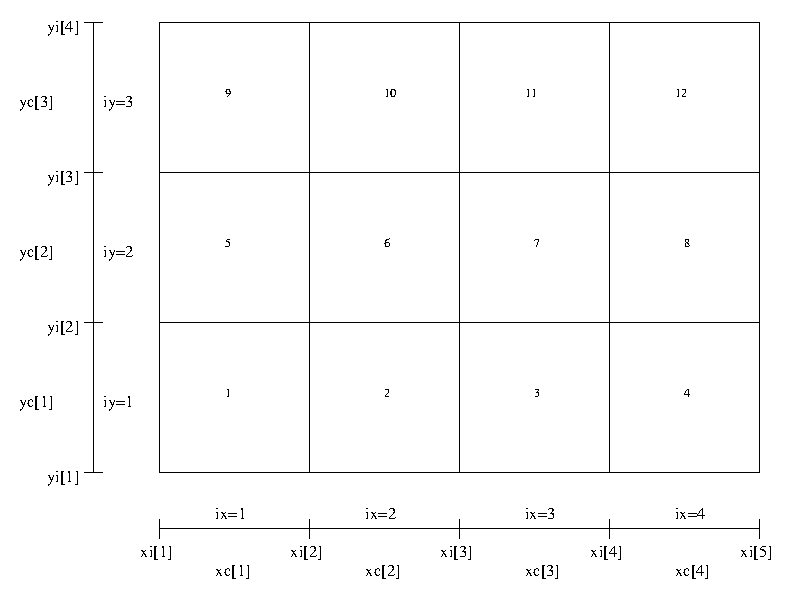
\includegraphics[width=0.9\textwidth]{base_amr.eps}}
\caption{\label{fig-regular-grid-numbered}
Example of a regular 2-D grid with {\small\tt nx}=4 and {\small\tt ny}=3
(as Fig.~\ref{fig-regular-grid}), with the order of the cells shown as
numbers in the cells.
}
\end{figure}
%

\subsection{Example: {\small\tt dust\_density.inp} for an oct-tree refined grid}
For the case when you have an oct-tree refined grid (see Sections
\ref{sec-amr-grid-oct-tree} and \ref{sec-oct-tree-amr}), the order of the
numbers is the same as the order of the cells as specified in the {\small\tt
  amr\_grid.(u)inp} file (Section \ref{sec-grid-input}).  Let us take the
example of a simple 1x1x1 grid which is refined into 2x2x2 and for which the
(1,2,1) cell is refined again in 2x2x2 (this is exactly the same example as
shown in Section \ref{sec-amr-grid-oct-tree}, and for which the {\small\tt
  amr\_grid.inp} is given in that section). Let us also assume that we have
only one dust species. Then the {\small\tt dust\_density.inp} file would be:
\begin{asciibox}\begin{verbatim}
iformat                                  <=== Typically 1 at present
15                                       <=== 2x2x2 - 1 + 2x2x2 = 15
1                                        <=== Let us take just one dust spec
density[1,1,1]                           <=== This is the first base grid cell
density[2,1,1]
density[1,2,1;1,1,1]                     <=== This is the first refined cell
density[1,2,1;2,1,1]
density[1,2,1;1,2,1]
density[1,2,1;1,2,1]
density[1,2,1;1,1,2]
density[1,2,1;2,1,2]
density[1,2,1;1,2,2]
density[1,2,1;1,2,2]                     <=== This is the last refined cell
density[2,2,1]
density[1,1,2]
density[2,1,2]
density[1,2,2]
density[2,2,2]                           <=== This is the last base grid cell
\end{verbatim}\end{asciibox}
A more complex example is shown in Fig.~\ref{fig-oct-tree-amr-numbered}.
An unformatted version is also available, in the standard way (see above).
%
\begin{figure}
\centerline{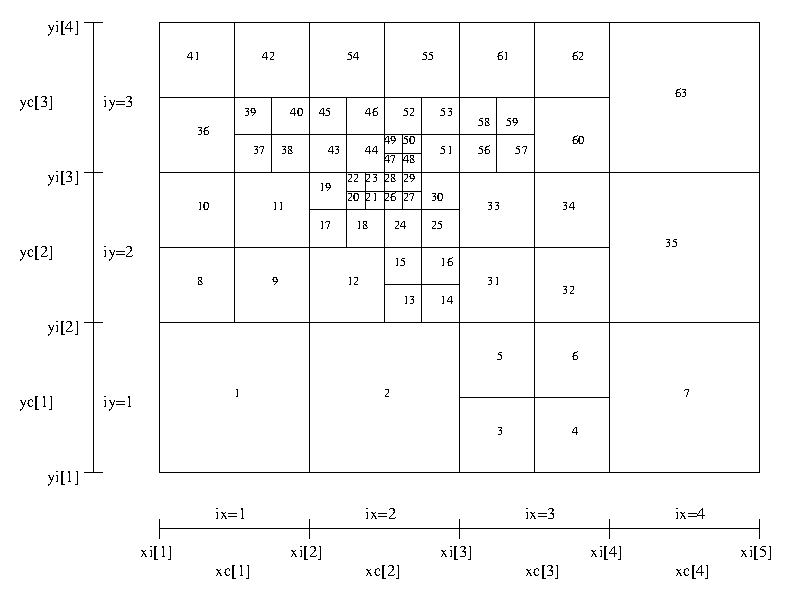
\includegraphics[width=0.9\textwidth]{oct_tree_amr.eps}}
\caption{\label{fig-oct-tree-amr-numbered}
Example of a 2-D grid with oct-tree refinement (as Fig.~\ref{fig-oct-tree-amr})
with the order of the cells shown as numbers in the cells.
}
\end{figure}



\subsection{Example: {\small\tt dust\_density.inp} for a layer-style refined grid}
For the case when you have an layer-style refined grid (see Sections
\ref{sec-amr-grid-layered} and \ref{sec-layered-amr}) you specify the
density in a series of regular boxes (=layers). The first box is the base
grid, the second the first layer, the third the second layer etc.  The value
{\small\tt nrcells} now tells the combined sizes of the all the boxes. If we
take the second example of Section \ref{sec-amr-grid-layered}: a simple 2-D
4x4 grid which has a refinement patch (=layer) in the middle of again 4x4
cells, and again one patch of 4x4 this time, however, starting in the upper
left corner (see the {\small\tt amr\_grid.inp} file given in Section
\ref{sec-amr-grid-layered}), then the {\small\tt dust\_density.inp} file
has the following form:
\begin{asciibox}\begin{verbatim}
iformat                                  <=== Typically 1 at present
48                                       <=== 4x4 + 4x4 + 4x4 = 48
1                                        <=== Let us take just one dust spec
density[1,1,1,layer=0]
density[2,1,1,layer=0]
density[3,1,1,layer=0]
density[4,1,1,layer=0]
density[1,2,1,layer=0]
density[2,2,1,layer=0]                   <=== This a redundant value
density[3,2,1,layer=0]                   <=== This a redundant value
density[4,2,1,layer=0]
density[1,3,1,layer=0]
density[2,3,1,layer=0]                   <=== This a redundant value
density[3,3,1,layer=0]                   <=== This a redundant value
density[4,3,1,layer=0]
density[1,4,1,layer=0]
density[2,4,1,layer=0]
density[3,4,1,layer=0]
density[4,4,1,layer=0]
density[1,1,1,layer=1]                   <=== This a redundant value
density[2,1,1,layer=1]                   <=== This a redundant value
density[3,1,1,layer=1]
density[4,1,1,layer=1]
density[1,2,1,layer=1]                   <=== This a redundant value
density[2,2,1,layer=1]                   <=== This a redundant value
density[3,2,1,layer=1]
density[4,2,1,layer=1]
density[1,3,1,layer=1]
density[2,3,1,layer=1]
density[3,3,1,layer=1]
density[4,3,1,layer=1]
density[1,4,1,layer=1]
density[2,4,1,layer=1]
density[3,4,1,layer=1]
density[4,4,1,layer=1]
density[1,1,1,layer=2]
density[2,1,1,layer=2]
density[3,1,1,layer=2]
density[4,1,1,layer=2]
density[1,2,1,layer=2]
density[2,2,1,layer=2]
density[3,2,1,layer=2]
density[4,2,1,layer=2]
density[1,3,1,layer=2]
density[2,3,1,layer=2]
density[3,3,1,layer=2]
density[4,3,1,layer=2]
density[1,4,1,layer=2]
density[2,4,1,layer=2]
density[3,4,1,layer=2]
density[4,4,1,layer=2]
\end{verbatim}\end{asciibox}
An unformatted version is also available, in the standard way (see above).

It is clear that 48 is now the total number of values to be read, which is
16 values for layer 0 (= base grid), 16 values for layer 1 and 16 values
for layer 2. It is also clear that some values are redundant (they can
have any value, does not matter). But it at least assures that each data
block is a simple regular data block, which is easier to handle. Note that
these values (marked as redundant in the above example) {\em must} be 
present in the file, but they can have any value you like (typically 0).

Note that if you have multiple species of dust then we will still have
48 as the value of {\small\tt nrcells}. The number of values to be read,
if you have 2 dust species, is then simply 2*{\small\tt nrcells} = 2*48 = 96.



\section{INPUT/OUTPUT: dust\_temperature.dat}
The dust temperature file is an intermediate result of RADMC-3D and follows
from the thermal Monte Carlo simulation. The name of this file is {\small\tt
  dust\_temperature.dat} (see Chapter \ref{chap-binary-io} for the binary
version of this file, which is more compact). It can be used by the user for
other purposes (e.g.\ determination of chemical reaction rates), but also by
RADMC-3D itself when making ray-traced images and/or spectra. The user can
also produce his/her own {\small\tt dust\_temperature.dat} file (without
invoking the Monte Carlo computation) if she/he has her/his own way of
computing the dust temperature.

The structure of this file is identical to that of {\small\tt
  dust\_density.inp} (Section \ref{sec-dustdens}), but with density replaced
by temperature. We refer to section \ref{sec-dustdens} for the details.



\section{INPUT/OUTPUT (only if required): electron\_numdens.inp}
For various gasopacity issues (see Chapter \ref{chap-gas-continuum}) the
number density of free electrons may be required. This is given in a file
called {\small\tt electron\_numdens.inp} (see Chapter \ref{chap-binary-io}
for the binary version of this file, which is more compact, and which you
can use instead of the ascii versions).  The structure of this file is
identical to that of {\small\tt dust\_density.inp} (Section
\ref{sec-dustdens}), but with density replaced by the electron number
density in units of 1/cm$^3$. We refer to chapter \ref{chap-gas-continuum}
for the details. 


\section{INPUT/OUTPUT (only if required): ion\_numdens.inp}
For various gasopacity issues (see Chapter \ref{chap-gas-continuum}) the
number density of ions may be required. This is given in a file
called {\small\tt ion\_numdens.inp} (see Chapter \ref{chap-binary-io}
for the binary version of this file, which is more compact, and which you
can use instead of the ascii versions). The structure of this file is
identical to that of {\small\tt dust\_density.inp} (Section
\ref{sec-dustdens}), but with density replaced by the ion number density in
units of 1/cm$^3$. Here we need the overal ion number density.  We refer to
chapter \ref{chap-gas-continuum} for the details. 


\section{INPUT (mostly required): stars.inp}
\label{sec-stars}
This is the file that specifies the number of stars, their positions,
radii, and spectra. Stars are sources of netto energy. For the dust
continuum Monte Carlo simulation these are a source of photon packages.
This file exists only in formatted (ascii) style. Its structure is:
\begin{asciibox}\begin{verbatim}
iformat                           <=== Put this to 2 !
nstars        nlam
rstar[1]      mstar[1]      xstar[1]      ystar[1]      zstar[1]
  .             .              .             .             .
  .             .              .             .             .
rstar[nstars  mstar[nstars] xstar[nstars] ystar[nstars] zstar[nstars]
lambda[1]
  .
  .
lambda[nlam]
flux[1,star=1]
  .
  .
flux[nlam,star=1]
flux[1,star=2]
  .
  .
flux[nlam,star=2]
  .
  .
  .
  .
flux[nlam,star=nstar]
\end{verbatim}\end{asciibox}

which is valid only if {\small\tt iformat}==2. The meaning of the variables:
\begin{itemize}
\item[] {\small\tt\bf iformat:} The format number, at present better keep it at 2. 
  If you put it to 1, the list of wavelengths (see below) will instead be
  a list of frequencies in Herz. 
\item[] {\small\tt\bf nstars:} The number of stars you wish to specify.
\item[] {\small\tt\bf nlam:} The number of frequency points for the stellar
  spectra. At present this must be identical to the number of walvelength
  points in the file {\small\tt wavelength\_micron.inp} (see Section \ref{sec-wavelengths}). 
\item[] {\small\tt\bf rstar[i]:} The radius of star $i$ in centimeters.
\item[] {\small\tt\bf mstar[i]:} The mass of star $i$ in grams. This is not
  important for the current version of RADMC-3D, but may be in the
  future.
\item[] {\small\tt\bf xstar[i]:} The {\small\tt x}-coordinate of star $i$ in centimeters.
\item[] {\small\tt\bf ystar[i]:} The {\small\tt y}-coordinate of star $i$ in centimeters.
\item[] {\small\tt\bf zstar[i]:} The {\small\tt z}-coordinate of star $i$ in centimeters.
\item[] {\small\tt\bf lambda[i]:} Wavelength point $i$ (where $i\in [1,${\small\tt
    nlam}$]$) in microns. This must be identical (!) to the equivalent
  point in the file {\small\tt wavelength\_micron.inp} (see Section \ref{sec-wavelengths}). If not, an error occurs.
\item[] {\small\tt\bf flux[i,star=n]:} The flux $F_\nu$ at wavelength point $i$
  for star $n$ in units of erg cm$^{-2}$ s$^{-1}$ Hz$^{-1}$ as seen from a
  distance of 1 parsec = $3.08572\times 10^{18}$ cm (for normalization).
\end{itemize}

\noindent Sometimes it may be sufficient to assume simple blackbody spectra
for these stars. If for any of the stars the first (!) flux number 
({\small\tt flux[1,star=n]}) is negative, then the absolute value of this number
is taken to be the blackbody temperature of the star, and no further values
for this star are read. Example:
\begin{asciibox}\begin{verbatim}
2
1            100
6.96e10      1.99e33        0.      0.    0.
0.1
  .
  .
1000.
-5780.
\end{verbatim}\end{asciibox}
will make one star, at the center of the coordinate system, with one solar
radius, one solar mass, on a wavelength grid ranging from 0.1 micron to 1000
micron (100 wavelength points) and with a blackbody spectrum with a
temperature equal to the effective temperature of the sun.

Note: The position of a star can be both inside and outside of the 
computational domain.


\section{INPUT (optional): stellarsrc\_templates.inp}
\label{sec-stellarsrc-templates}
This is the file that specifies the template spectra for the smooth stellar
source distributions. See Section \ref{sec-distrib-of-stars}.
The file exists only in formatted (ascii) style. Its structure is:
\begin{asciibox}\begin{verbatim}
iformat                           <=== Put this to 2 !
ntempl
nlam
lambda[1]
  .
  .
lambda[nlam]
flux[1,templ=1]
  .
  .
flux[nlam,templ=1]
flux[1,templ=2]
  .
  .
flux[nlam,templ=2]
  .
  .
  .
  .
flux[nlam,templ=ntempl]
\end{verbatim}\end{asciibox}

which is valid only if {\small\tt iformat}==2. The meaning of the variables:
\begin{itemize}
\item[] {\small\tt\bf iformat:} The format number, at present better keep it at 2. 
  If you put it to 1, the list of wavelengths (see below) will instead be
  a list of frequencies in Herz. 
\item[] {\small\tt\bf ntempl:} The number of stellar templates you wish to specify.
\item[] {\small\tt\bf nlam:} The number of frequency points for the stellar
  template spectra. At present this must be identical to the number of
  walvelength points in the file {\small\tt wavelength\_micron.inp} (see
  Section \ref{sec-wavelengths}).
\item[] {\small\tt\bf lambda[i]:} Wavelength point $i$ (where $i\in
  [1,${\small\tt nlam}$]$) in microns. This must be identical (!) to the
  equivalent point in the file {\small\tt wavelength\_micron.inp} (see
  Section \ref{sec-wavelengths}). If not, an error occurs.
\item[] {\small\tt\bf flux[i,templ=n]:} The ``flux'' at wavelength $i$ for
  stellar template $n$. The units are somewhat tricky. It is given in units
  of erg / sec / Hz / gram-of-star. So multiply this by the density of
  stars in units of gram-of-star / cm$^3$, and divide by 4*pi to get the
  stellar source function in units of erg / src / Hz / cm$^3$ / steradian.
\end{itemize}

\noindent Sometimes it may be sufficient to assume simple blackbody spectra
for these stellar sources. If for any of the stellar sources the first (!)
flux number ({\small\tt flux[1,templ=n]}) is negative, then the absolute
value of this number is taken to be the blackbody temperature of the stellar
source, and the following two numbers are interpreted as the stellar radius
and stellar mass respectively. From that, RADMC-3D will then internally
compute the stellar template. Example:
\begin{asciibox}\begin{verbatim}
2
1            
100
0.1
  .
  .
1000.
-5780.
6.9600000e+10   
1.9889200e+33
\end{verbatim}\end{asciibox}
will tell RADMC-3D that there is just one stellar template, assumed to have
a blackbody spectrum with solar effective temperature. Each star of this
template has one solar radius, one solar mass.



\section{INPUT (optional): stellarsrc\_density.inp}
\label{sec-stellarsrc-density}
%
This is the file that contains the smooth stellar source densities. If you
have the file {\small\tt stellarsrc\_templates.inp} specified (see Section
\ref{sec-stellarsrc-templates}) then you {\em must} also specify {\small\tt
  stellarsrc\_density.inp} (or its binary form, see Chapter
\ref{chap-binary-io}).  The format of this file is very similar to
{\small\tt dust\_density.inp} (Section \ref{sec-dustdens}), but instead
different dust species, we have different templates.  For the rest we refer
to Section \ref{sec-dustdens} for the format.  Just replace {\small\tt
  ispec} (the dust species) with {\small\tt itempl} (the template). 


\section{INPUT (optional): external\_source.inp}
\label{sec-ext-src-inp}
This is the file that specifies the spectrum and intensity of the
external radiation field, i.e.\ the ``interstellar radiation field''
(see Section \ref{sec-external-source}). Its structure is:
\begin{asciibox}\begin{verbatim}
iformat                           <=== Put this to 2 !
nlam
lambda[1]
  .
  .
lambda[nlam]
Intensity[1]
  .
  .
Intensity[nlam]
\end{verbatim}\end{asciibox}

which is valid only if {\small\tt iformat}==2. The meaning of the variables:
\begin{itemize}
\item[] {\small\tt\bf iformat:} The format number, at present better keep it at 2. 
  If you put it to 1, the list of wavelengths (see below) will instead be
  a list of frequencies in Herz. 
\item[] {\small\tt\bf nlam:} The number of frequency points for the stellar
  template spectra. At present this must be identical to the number of
  walvelength points in the file {\small\tt wavelength\_micron.inp} (see
  Section \ref{sec-wavelengths}).
\item[] {\small\tt\bf lambda[i]:} Wavelength point $i$ (where $i\in
  [1,${\small\tt nlam}$]$) in microns. This must be identical (!) to the
  equivalent point in the file {\small\tt wavelength\_micron.inp} (see
  Section \ref{sec-wavelengths}). If not, an error occurs.
\item[] {\small\tt\bf Intensity[i]:} The intensity of the radiation field at
  wavelength $i$ in units of erg / cm$^2$ / sec / Hz / steradian.
\end{itemize}


\section{INPUT (optional): heatsource.inp}
\label{sec-heatsource}
%
This file, if present (it is an optional file!), gives the internal heat
source of the gas-dust mixture in every cell. For formatted style
({\small\tt heatsource.inp}) the structure of this file is as follows.:
\begin{asciibox}\begin{verbatim}
iformat                                  <=== Typically 1 at present
nrcells
heatsource[1]
..
heatsource[nrcells]
\end{verbatim}\end{asciibox}
As with most input/output files of RADMC-3D, you can also specify the input
data in binary form ({\small\tt heatsource.binp}), see Chapter
\ref{chap-binary-io}.

The physical unit of {\small\tt heatsource} is
$\mathrm{erg}\,\mathrm{cm}^{-3}\,\mathrm{s}^{-1}$. The total luminosity of
the heat source would then be the sum over all cells of {\small\tt
  heatsource} times the cell volume. 


\section{INPUT (required): wavelength\_micron.inp}
\label{sec-wavelengths}
%
This is the file that sets the discrete wavelength points for the continuum
radiative transfer calculations. Note that this is not the same as the
wavelength grid used for e.g.\ line radiative transfer.  See Section \ref{sec-camera-wavelengths} and/or Chapter \ref{chap-line-transfer} for
that. This file is only in formatted (ascii) style. It's structure is:
\begin{asciibox}\begin{verbatim}
nlam
lambda[1]
  .
  .
lambda[nlam]
\end{verbatim}\end{asciibox}
where
\begin{itemize}
\item[] {\small\tt\bf nlam:} The number of frequency points for the stellar
  spectra.
\item[] {\small\tt\bf lambda[i]:} Wavelength point $i$ (where $i\in [1,${\small\tt
    nlam}$]$) in microns.
\end{itemize}
The list of wavelengths can be in increasing order or decreasing order, but
must be monotonically increasing/decreasing. 

{\bf IMPORTANT:} It is important to keep in mind that the wavelength
coverage must include the wavelengths at which the stellar spectra have most
of their energy, and at which the dust cools predominantly.  This in
practice means that this should go all the way from 0.1 $\mu$m to 1000
$\mu$m, typically logarithmically spaced (i.e.~equally spaced in
log$\lambda$). A smaller coverage will cause serious problems in the Monte
Carlo run and dust temperatures may then be severely miscalculated. Note
that the 0.1 $\mu$m is OK for stellar temperatures below 10000 K. For higher
temperatures a shorter wavelength lower limit must be used.




\section{INPUT (optional): camera\_wavelength\_micron.inp}
\label{sec-camera-wavelengths}
%
The wavelength points in the {\small\tt wavelength\_micron.inp} file are the
global continuum wavelength points. On this grid the continuum transfer is
done. However, there may be various reasons why the user may want to
generate spectra on a different (usually more finely spaced) wavelength
grid, or make an image at a wavelength that is not available in the global
continuum wavelength grid. Rather than redoing the entire model with a
different {\small\tt wavelength\_micron.inp}, which may involve a lot of
reorganization and recomputation, the user can specify a file called {\small\tt
  camera\_wavelength\_micron.inp}. If this file exists, it will be read into
RADMC-3D, and the user can now ask RADMC-3D to make images in those
wavelength or make a spectrum in those wavelengths. 

If the user wants to make images or spectra of a model that involves gas
lines (such as atomic lines or molecular rotational and/or ro-vibrational
lines), the use of a {\small\tt camera\_wavelength\_micron.inp} file allows
the user to do the line+dust transfer (gas lines plus the continuum) on this
specific wavelength grid. For line transfer there are also other ways by
which the user can specify the wavelength grid (see Chapter
\ref{chap-line-transfer}), and it is left to the user to choose which method
to use.

The structure of the {\small\tt camera\_wavelength\_micron.inp} file is
identical to that of {\small\tt wavelength\_micron.inp} (see Section
\ref{sec-wavelengths}).

Note that there are also various other ways by which the user can let
RADMC-3D choose wavelength points, many of which may be even simpler
and more preferable than the method described here. See Section
\ref{sec-set-camera-frequencies}.



\section{INPUT (required for dust transfer): dustopac.inp and dustkappa\_*.inp or dustkapscatmat\_*.inp or dust\_optnk\_*.inp}
\label{sec-opacities}
These files specify the dust opacities to be used. More than one can be
specified, meaning that there will be more than one co-existing dust
species. Each of these species will have its own dust density specified
(see Section \ref{sec-dustdens}). The opacity of each species is specified
in a separate file for each species. The {\small\tt dustopac.inp} file tells which 
file to read for each of these species.

\subsection{The dustopac.inp file}\label{sec-dustopac-inp-file}
The file {\small\tt dustopac.inp} has the following structure, where an example
of 2 separate dust species is used:
\begin{asciibox}\begin{verbatim}
iformat                          <=== Put this to 2
nspec
-----------------------------
inputstyle[1]
iquantum[1]                      <=== Put to 0 in this example
<name of dust species 1>
-----------------------------
inputstyle[2]
iquantum[2]                      <=== Put to 0 in this example
<name of dust species 2>
\end{verbatim}\end{asciibox}
where:
\begin{itemize}
\item[] {\small\tt\bf iformat:} Currently the format number is 2, and in this manual
  we always assume it is 2.
\item[] {\small\tt\bf nspec:} The number of dust species that will be loaded.
\item[] {\small\tt\bf inputstyle[i]:} This number tells in which form the dust
  opacity of dust species $i$ is to be read:
  \begin{itemize}
  \item[{\em 1}] Use the {\small\tt dustkappa\_$<$name$>$.inp} input file
    style (see Section \ref{sec-dustkappa-files}). 
  \item[{\em 10}] Use the {\small\tt dustkapscatmat\_$<$name$>$.inp} input
    file style (see Section \ref{sec-dustkapscatmat-files}).
%  \item[{\em 100}] Use the {\small\tt dustoptnk\_$<$name$>$.inp} input file
%    style (see below). Here the optical constants are read on their own
%    wavelength grid. Using Mie theory or CDE the opacities are then computed
%    internally and mapped onto the global continuum wavelength grid from the
%    {\small\tt wavelength\_micron.inp} file.
  \item[{\em -1}] Use the {\small\tt dustopac\_$<$name$>$.inp} input file
    style (see Section \ref{sec-dustopac-oldstyle}). This is just a backward
    compatibility mode. Should be avoided if possible.
  \end{itemize}
\item[] {\small\tt\bf iquantum[i]:} For normal thermal grains this is 0. If,
  however, this grain species is supposed to be treated as a quantum-heated
  grain, then non-zero values are to be specified. {\em NOTE: At the moment
    the quantum heating is not yet implemented. Will be done in the near
    future. Until then, please set this to 0!}
\item[] {\small\tt\bf $<$name of dust species i$>$:} This is the name of the
  dust species (without blank spaces). This name is then glued to the base
  name of the opacity file (see above). For instance, if the name is
  {\small\tt enstatite}, and {\small\tt inputstyle}==1, then the file to be
  read is {\small\tt dustkappa\_enstatite.inp}.
\end{itemize}

 
\subsection{The dustkappa\_$<$name$>$.inp files}
\label{sec-dustkappa-files}
%
If you wish to use dust opacities that include the mass-weighted absorption
opacity $\kappa_{\mathrm{abs}}$, the (optionally) mass-weighted scattering
opacity $\kappa_{\mathrm{scat}}$, and (optionally) the anisotropy factor $g$
for scattering, you can do this with a file {\small\tt
  dustkappa\_$<$name$>$.inp} (set input style to 1 in {\small\tt
  dustopac.inp}, see Section \ref{sec-dustopac-inp-file}). With this kind of
opacity scattering is included either isotropically or using the
Henyey-Greenstein function.  Using an opacity of this kind does {\em not}
allow for full realistic scattering phase functions nor for
polarization. For that, you need {\small\tt dustkapscatmat\_$<$name$>$.inp}
files (see Section \ref{sec-dustkapscatmat-files}). Please refer to Section
\ref{sec-scattering} for more information about how RADMC-3D treats
scattering.

If for dust species {\small\tt $<$name$>$} the {\small\tt inputstyle} in the 
{\small\tt dustopac.inp} file is set to 1, then the file 
{\small\tt dustkappa\_$<$name$>$.inp}
is sought and read. The structure of this file is:
\begin{asciibox}\begin{verbatim}
# Any amount of arbitrary
# comment lines that tell which opacity this is.
# Each comment line must start with an # or ; or ! character
iformat                     <== This example is for iformat==3
nlam
lambda[1]        kappa_abs[1]       kappa_scat[1]      g[1]
   .                  .                  .              .
   .                  .                  .              .
lambda[nlam]    kappa_abs[nlam]   kappa_scat[nlam]    g[nlam]
\end{verbatim}\end{asciibox}
The meaning of these entries is:
\begin{itemize}
\item[] {\small\tt\bf iformat:} If iformat==1, then only the lambda and
  kappa\_abs colums are present. In that case the scattering opacity is
  assumed to be 0, i.e.\ a zero albedo is assumed. If iformat==2 also
  kappa\_scat is read (third column). If iformat==3 (which is what is used in
  the above example) then {\em also} the anisotropy factor $g$ is included.
\item[] {\small\tt\bf nlam:} The number of wavelength points in this file. This
  can be any number, and does not have to be the same as those of the
  {\small\tt wavelength\_micron.inp}. It is typically advisable to have a rather
  large number of wavelength points.
\item[] {\small\tt\bf lambda[i]:} The wavelength point $i$ in micron. This does
  not have to be (and indeed typically is not) the same as the values in the
  {\small\tt wavelength\_micron.inp} file. Also for each opacity this list of
  wavelengths can be different (and can be a different quantity of points).
\item[] {\small\tt\bf kappa\_abs[i]:} The absorption opacity $\kappa_{\mathrm{abs}}$ in units of cm$^2$ per gram of dust.
\item[] {\small\tt\bf kappa\_scat[i]:} The scattering opacity $\kappa_{\mathrm{abs}}$ in units of cm$^2$
  per gram of dust. Note that this column should only be included if 
  iformat==2 or higher. 
\item[] {\small\tt\bf g[ilam]:} The mean scattering angle
  $\langle\cos(\theta)\rangle$, often called $g$. This will be used by
  RADMC-3D in the Henyey-Greenstein scattering phase function. Note that
  this column should only be included if iformat==3 or higher.
\end{itemize}
Once this file is read, the opacities will be mapped onto the global
wavelength grid of the {\small\tt wavelength\_micron.inp} file. Since this mapping
always involve uncertainties and errors, a file {\small\tt
  dustkappa\_$<$name$>$.inp\_used} is created which lists the opacity how it
is remapped onto the global wavelength grid. This is only for you as the
user, so that you can verify what RADMC-3D has internally done. Note that if
the upper or lower edges of the wavelength domain of the {\small\tt
  dustkappa\_$<$name$>$.inp} file is within the domain of the {\small\tt
  wavelength\_micron.inp} grid, some extrapolation will have to be done.  At
short wavelength this will simply be constant extrapolation while at long
wavelength a powerlaw extrapolation is done. Have a look at the {\small\tt
  dustkappa\_$<$name$>$.inp\_used} file to see how RADMC-3D has done this
in your particular case.

\subsection{The dustkapscatmat\_$<$name$>$.inp files}
\label{sec-dustkapscatmat-files}
%
If you wish to treat scattering in a more realistic way than just the
Henyey-Greenstein non-polarized way, then you must provide RADMC-3D with
more information than is present in the {\small\tt dustkappa\_xxx.inp}
files: RADMC-3D will need the full scattering M\"uller matrix for all angles
of scattering (see e.g.\ the books by Mishchenko, or by Bohren \& Huffman or
by van de Hulst). For {\em randomly oriented particles} only 6 of these
matrix elements can be non-zero: $Z_{11}$, $Z_{12}=Z_{21}$, $Z_{22}$,
$Z_{33}$, $Z_{34}=-Z_{43}$, $Z_{44}$, where 1,2,3,4 represent the I,Q,U,V
Stokes parameters. Moreover, for randomly oriented particles there is only 1
scattering angle involved: the angle between the incoming and outgoing
radiation of the scattering event. This means that we must give RADMC-3D,
(for every wavelength and for a discrete set of scattering angles) a list of
values of these 6 matrix elements. These can be provided in a file
{\small\tt dustkapscatmat\_xxx.inp} (set input style to 10 in {\small\tt
  dustopac.inp}, see Section \ref{sec-dustopac-inp-file}) which comes {\em
  instead of} the {\small\tt dustkappa\_xxx.inp} file. Please refer to
Section \ref{sec-scattering} for more information about how RADMC-3D treats
scattering.

If for dust species {\small\tt $<$name$>$} the {\small\tt inputstyle} in the 
{\small\tt dustopac.inp} file is set to 10, then the file 
{\small\tt dustkapscatmat\_$<$name$>$.inp}
is sought and read. The structure of this file is:
\begin{asciibox}\begin{verbatim}
# Any amount of arbitrary
# comment lines that tell which opacity this is.
# Each comment line must start with an # or ; or ! character
iformat            <== Format number must be 1
nlam
nang               <== A reasonable value is 181 (e.g. angle = 0.0,1.0,...,180.0)

lambda[1]        kappa_abs[1]       kappa_scat[1]     g[1]
   .                  .                  .             .
   .                  .                  .             .
lambda[nlam]    kappa_abs[nlam]   kappa_scat[nlam]   g[nlam]

angle_in_degrees[1]
   .
   .
angle_in_degrees[nang]

Z_11  Z_12  Z_22  Z_33  Z_34  Z_44   [all for ilam=1 and iang=1]
Z_11  Z_12  Z_22  Z_33  Z_34  Z_44   [all for ilam=1 and iang=2]
Z_11  Z_12  Z_22  Z_33  Z_34  Z_44   [all for ilam=1 and iang=3]
 .     .     .     .     .     .
 .     .     .     .     .     .
Z_11  Z_12  Z_22  Z_33  Z_34  Z_44   [all for ilam=1 and iang=nang]

Z_11  Z_12  Z_22  Z_33  Z_34  Z_44   [all for ilam=2 and iang=1]
 .     .     .     .     .     .
 .     .     .     .     .     .
Z_11  Z_12  Z_22  Z_33  Z_34  Z_44   [all for ilam=2 and iang=nang]

....
....
....

Z_11  Z_12  Z_22  Z_33  Z_34  Z_44   [all for ilam=nlam and iang=1]
 .     .     .     .     .     .
 .     .     .     .     .     .
Z_11  Z_12  Z_22  Z_33  Z_34  Z_44   [all for ilam=nlam and iang=nang]
\end{verbatim}\end{asciibox}
The meaning of these entries is:
\begin{itemize}
\item[] {\small\tt\bf iformat:} For now this value should remain 1.
\item[] {\small\tt\bf nlam:} The number of wavelength points in this file. This
  can be any number, and does not have to be the same as those of the
  {\small\tt wavelength\_micron.inp}. It is typically advisable to have a rather
  large number of wavelength points.
\item[] {\small\tt\bf nang:} The number of scattering angle sampling points.
  This should be large enough that a proper integration over scattering angle
  can be carried out reliably. A reasonable value is 181, so that (for
  a regular grid in scattering angle $\theta$) you have as scattering angles
  $\theta=0,1,2,\cdots,180$ (in degrees). But if you have extremely forward-
  or backward peaked scattering, then maybe even 181 is not enough. 
\item[] {\small\tt\bf lambda[ilam]:} The wavelength point $ilam$ in micron. This does
  not have to be (and indeed typically is not) the same as the values in the
  {\small\tt wavelength\_micron.inp} file. Also for each opacity this list of
  wavelengths can be different (and can be a different quantity of points).
\item[] {\small\tt\bf angle\_in\_degrees[iang]:} The scattering angle
  sampling point $iang$ in degrees (0 degrees is perfect forward scattering,
  180 degrees is perfect backscattering). There should be {\small\tt nang}
  such points, where {\small\tt angle\_in\_degrees[1]} must be 0 and
  {\small\tt angle\_in\_degrees[nang]} must be 180. In between the angle
  grid can be anything, as long as it is monotonic.
\item[] {\small\tt\bf kappa\_abs[ilam]:} The absorption opacity $\kappa_{\mathrm{abs}}$ in units of cm$^2$ per gram of dust.
\item[] {\small\tt\bf kappa\_scat[ilam]:} The scattering opacity
  $\kappa_{\mathrm{scat}}$ in units of cm$^2$ per gram of dust. RADMC-3D can
  (and will) in fact calculate $\kappa_{\mathrm{scat}}$ from the scattering
  matrix elements. It will then check (for every wavelength) if that is the
  same as the value listed here. If the difference is small, it will simply
  adjust the {\small\tt\bf kappa\_scat[ilam]} value internally to get a
  perfect match. If it is larger than 1E-4 then it will, in addition to
  adjusting, make a warning. if it is larger than 1E-1, it will abort. Note
  that the fewer angles are used, the worse the match will be because the
  integration over angle will be worse.
\item[] {\small\tt\bf g[ilam]:} The mean scattering angle
  $\langle\cos(\theta)\rangle$, often called $g$. RADMC-3D can (and will) in
  fact calculate $g$ from the scattering matrix elements. Like with
  {\small\tt\bf kappa\_scat[ilam]} it will adjust if the difference is not
  too large and it will complain or abort if the difference is larger than
  some limit.
\item[] {\small\tt Z\_{xx}} These are the scattering matrix elements
  in units of cm$^2$ gram$^{-1}$ ster$^{-1}$ (i.e.\ they are angular
  differential cross sections). See Section \ref{sec-scattering} for
  more details.
\end{itemize}

NOTE: This only allows the treatment of {\em randomly oriented
  particles}. RADMC-3D does not, for now, have the capability of treating
scattering off fixed-oriented particles\footnote{In fact, for oriented
  particles it would be impractical to use dust opacity files of this kind,
  since we would then have at least {\em three} scattering angles, which
  would require huge table. In that case it would be presumably necessary to
  compute the matrix elements on-the-fly.}.

Note that the scattering-angle grid of the {\small\tt dustkapscatmat\_xxx.inp}
files can be chosen non-regular, e.g.\ to put a more finely spaced grid
close to $\theta=0$ (forward scattering) and $\theta=\pi$ (backscattering).
This can be useful for large grains and/or short wavelengths, where forward
scattering can be extremely strongly peaked. Since multiple dust species
can each have a different scattering $\theta$-grid, it requires you to
give an additional file to {\small\tt RADMC-3D} that represents the 
scattering $\theta$-grid for all grains. This file is called 
{\small\tt scattering\_angular\_grid.inp}. The format is as follows:
\begin{asciibox}\begin{verbatim}
1            <=== Format number, must be 1
181          <=== Nr of theta grid points
0.0          <=== First angle (in degrees). Must be 0
1.0          
2.0          
...
...
...
179.0        
180.0        <=== Last angle (in degrees). Must be 180
\end{verbatim}\end{asciibox}
{\bf NOTE:} This file is not compulsory. If it is not given, then 
{\small\tt RADMC-3D} will make its own internal scattering angle grid.

\subsection{The dustopac\_$<$name$>$.inp files: Backward compatibility with RADMC-2D}
\label{sec-dustopac-oldstyle}
If you want to be able to redo a model from the old RADMC (2D-version) code
with RADMC-3D, you require RADMC-3D to be able to read the old style 
dust opacity files {\small\tt dustopac\_$<$name$>$.inp}.

If for dust species {\small\tt $<$name$>$} the {\small\tt inputstyle} in the 
{\small\tt dustopac.inp} file is set to -1, then the file {\small\tt dustopac\_$<$name$>$.inp}
is sought and read. The structure of this file is:
\begin{asciibox}\begin{verbatim}
nlam   dummy
kappa_abs[1]
  .
  .
kappa_abs[nlam]
kappa_scat[1]
  .
  .
kappa_scat[nlam]
\end{verbatim}\end{asciibox}
The meaning of these entries is:
\begin{itemize}
\item[] {\small\tt\bf nlam:} The number of frequency (wavelength) points. This
  must be {\em identical} to those of the {\small\tt wavelength\_micron.inp} file
  or else the code stops.
\item[] {\small\tt\bf dummy:} Put this number to 1. It is here for historic
  reasons (and backward compatibility with older RADMC incarnations).
\item[] {\small\tt\bf kappa\_abs[i]:} The absorption opacity at wavelength point
  $i$ of the {\small\tt wavelength\_micron.inp} wavelength grid, in units of
  cm$^2$ per gram of dust.
\item[] {\small\tt\bf kappa\_scat[i]:} The scattering opacity at wavelength point
  $i$ of the {\small\tt wavelength\_micron.inp} wavelength grid, in units of
  cm$^2$ per gram of dust. {\em NOTE: Here isotropic scattering is assumed.}
\end{itemize}
Note that the opacities listed in this kind of file belong to the wavelength
points in the file {\small\tt wavelength\_micron.inp}. So if you change the {\small\tt
  wavelength\_micron.inp} file, you also must change the
{\small\tt dustopac\_$<$name$>$.inp} files. This is why this kind of opacity
specification is not recommended.


% \subsection{The dustoptnk\_$<$name$>$.inp files}
% If for dust species {\small\tt $<$name$>$} the {\small\tt inputstyle} in the
% {\small\tt dustopac.inp} file is set to 100, then the file
% dustoptnk\_$<$name$>$.inp is sought and read.
% 
% {\em NOTE: For now we discourage this mode as it is insufficiently tested.}



\section{OUTPUT: spectrum.out}
\label{sec-output-spectrum-out}
%
Any spectrum that is made with RADMC-3D will be either called
{\small\tt spectrum.out} or {\em spectrum\_$<$somename$>$.out} and will have
the following structure:
\begin{asciibox}\begin{verbatim}
iformat                      <=== For now this is 1
nlam

lambda[1]       flux[1]
   .              .
   .              .
lambda[nlam]   flux[nlam]
\end{verbatim}\end{asciibox}
where:
\begin{itemize}
\item[] {\small\tt\bf iformat:} This format number is currently set to 1.
\item[] {\small\tt\bf nlam:} The number of wavelength points in this spectrum.
  This does not necessarily have to be the same as those in the
  {\small\tt wavelength\_micron.inp} file. It can be any number.
\item[] {\small\tt\bf lambda[i]:} Wavelength in micron.  This does not necessarily
  have to be the same as those in the {\small\tt wavelength\_micron.inp} file.
  The wavelength grid of a spectrum file can be completely independent 
  of all other wavelength grids. For standard SED computations for the
  continuum typically these will be indeed the same as those in the
  {\small\tt wavelength\_micron.inp} file. But for line transfer or for 
  spectra based on the {\small\tt camera\_wavelength\_micron.inp} they are
  not. 
\item[] {\small\tt\bf flux[i]:} Flux in erg cm$^{-2}$ s$^{-1}$ Hz$^{-1}$ at this
  wavelength as measured at a standard distance of 1 parsec (just as a way
  of normalization).
\end{itemize}

{\em NOTE: Maybe in the future a new iformat version will be possible
where more telescope information is given in the spectrum file.}



\section{OUTPUT: image.out or image\_****.out}
\label{sec-image-out}
Any images that are produced by RADMC-3D will be written in a file called
{\small\tt image.out}. The file has the following structure (for the case
without Stokes parameters):
\begin{asciibox}\begin{verbatim}
iformat                      <=== For now this is 1 (or 2 for local observer mode)
im_nx        im_ny
nlam
pixsize_x    pixsize_y
lambda[1]  ......... lambda[nlam+1]

image[ix=1,iy=1,img=1]
image[ix=2,iy=1,img=1]
  .
  .
image[ix=im_nx,iy=1,img=1]
image[ix=1,iy=2,img=1]
  .
  .
image[ix=im_nx,iy=2,img=1]
image[ix=1,iy=im_ny,img=1]
  .
  .
  .
image[ix=im_nx,iy=im_ny,img=nlam]

image[ix=1,iy=1,img=1]
  .
  .
  .
  .
image[ix=im_nx,iy=im_ny,img=nlam]
\end{verbatim}\end{asciibox}
In most cases the nr of images (nr of wavelengths) is just 1, meaning only
one image is written (i.e.\ the img=2, .... img=nlam are not there, only
the img=1). The meaning of the various entries is:
\begin{itemize}
\item[] {\small\tt\bf iformat:} This format number is currently set to 1 
for images from an observer at infinity (default) and 2 for a local observer.
Note: For full-Stokes images it is 3, but then also the data changes a
bit, see below.
\item[] {\small\tt\bf im\_nx, im\_ny:} The number of pixels in x and in y
  direction of the image.
\item[] {\small\tt\bf nlam:} The number of images at different wavelengths that
are in this file. You can make a series of images at different wavelengths
in one go, and write them in this file. The wavelength belonging to each of
these images is listed below. The {\small\tt nlam} can be any number from 1 to
however large you want. Mostly one typically just makes an images at one
wavelength, meaning {\small\tt nlam}=1. 
\item[] {\small\tt\bf pixsize\_x, pixsize\_y:} The size of the pixels in cm
  (for an observer at infinity) or radian (for local observer mode).  This
  means that for the observer-at-infinity mode (default) the size is given
  in model units (distance within the 3-D model) and the user can, for any
  distance, convert this into arcseconds: pixel size in arcsec = ( pixel
  size in cm / 1.496E13) / (distance in parsec). The pixel size is the full
  size from the left of the pixel to the right of the pixel (or from bottom
  to top).
\item[] {\small\tt\bf lambda[i]:} Wavelengths in micron belonging to the various
  images in this file. In case {\small\tt nlam}=1 there will be here just a
  single number. Note that this set of wavelengths can be completely
  independent of all other wavelength grids. 
\item[] {\small\tt\bf image[ix,iy,img]:} Intensity in the image at pixel
  {\small\tt ix}, {\small\tt iy} at wavelength {\small\tt img} (of the above
  listed wavelength points) in units of erg cm$^{-2}$ s$^{-1}$ Hz$^{-1}$
  ster$^{-1}$. {\em Important:} The pixels are ordered from left to right
  (i.e.\ increasing $x$) in the inner loop, and from bottom to
  top (i.e.\ increasing $y$) in the outer loop.
\end{itemize}

You can also make images with full Stokes parameters. For this you must have
dust opacities that include the full scattering matrix, {\em and} you must
add the keyword {\small\tt stokes} to the {\small\tt radmc3d image} command
on the command-line. In that case the {\small\tt image.out} file has the
following form:
\begin{asciibox}\begin{verbatim}
iformat                      <=== For Stokes this is 3 
im_nx        im_ny
nlam
pixsize_x    pixsize_y
lambda[1]  ......... lambda[nlam+1]

image_I[ix=1,iy=1,img=1] image_Q[ix=1,iy=1,img=1] image_U[ix=1,iy=1,img=1] image_V[ix=1,iy=1,img=1]
  .
  .
image_I[ix=im_nx,iy=1,img=1] (and so forth for Q U and V)
image_I[ix=1,iy=2,img=1] (and so forth for Q U and V)
  .
  .
image_I[ix=im_nx,iy=2,img=1] (and so forth for Q U and V)
image_I[ix=1,iy=im_ny,img=1] (and so forth for Q U and V)
  .
  .
  .
image_I[ix=im_nx,iy=im_ny,img=nlam] (and so forth for Q U and V)

image_I[ix=1,iy=1,img=1] (and so forth for Q U and V)
  .
  .
  .
  .
image_I[ix=im_nx,iy=im_ny,img=nlam] (and so forth for Q U and V)
\end{verbatim}\end{asciibox}
That is: instead of 1 number per line we now have 4 numbers per line, which
are the four Stokes parameters. Note that {\small\tt iformat}=3 to indicate
that we have now all four Stokes parameters in the image.


\section{INPUT: (minor input files)}\label{sec-minor-input-files}
There is a number of lesser important input files, or input files that are
only read under certain circumstances (for instance when certain command
line options are given). Here they are described.

\subsection{The {\small\tt color\_inus.inp} file (required with comm-line option 'loadcolor')}
\label{sec-color-inus}
The file {\small\tt color\_inus.inp} will only be read by RADMC-3D if on the
command line the option {\small\tt loadcolor} or {\small\tt color} is
specified, and if the main action is {\small\tt image}.
\begin{asciibox}\begin{verbatim}
iformat                      <=== For now this is 1
nlam
ilam[1]
  .
  .
ilam[nlam]
\end{verbatim}\end{asciibox}
\begin{itemize}
\item[] {\small\tt\bf iformat:} This format number is currently set to 1.
\item[] {\bf\bf nlam:} Number of wavelength indices specified here.
\item[] {\bf\bf ilam[i]:} The wavelength index for image i (the wavelength
  index refers to the list of wavelengths in the {\small\tt
    wavelength\_micron.inp} file.
\end{itemize}


\subsection{INPUT: {\small\tt aperture\_info.inp}}
\label{sec-aperture-info-file}
%
If you wish to make spectra with wavelength-dependent collecting area, i.e.
aperture (see Section \ref{sec-aperture}), then you must prepare the
file {\small\tt aperture\_info.inp}. Here is its structure:
\begin{asciibox}\begin{verbatim}
iformat                      <=== For now this is 1
nlam
lambda[1]      rcol_as[1]
  .            .
  .            .
lambda[nlam]   rcol_as[nlam]
\end{verbatim}\end{asciibox}
with
\begin{itemize}
\item[] {\small\tt\bf iformat:} This format number is currently set to 1.
\item[] {\bf nlam:} Number of wavelength indices specified here. This
  does {\em not} have to be the same as the number of wavelength of a
  spectrum or the number of wavelengths specified in the file
  {\small\tt wavelength\_micron.inp}. It can be any number. 
\item[] {\bf lambda[i]:} Wavelength sampling point, in microns. You can use
  a course grid, as long as the range of wavelengths is large enough to
  encompass all wavelengths you may wish to include in spectra.
\item[] {\bf rcol\_as[i]:} The radius of the circular image mask used for
  the aperture model, in units of arcsec.
\end{itemize}




\section{For developers: some details on the internal workings}
There are several input files that can be quite large. Reading these files
into RADMC-3D memory can take time, so it is important not to read files
that are not required for the execution of the particular command at 
hand. For instance, if a model exists in which both dust and molecular
lines are included, but RADMC-3D is called to merely make a continuum
SED (which in RADMC-3D never includes the lines), then it would be a
waste of time to let RADMC-3D read all the gas velocity and temperature
data and level population data into memory if they are not used.

To avoid unnecessary reading of large files the reading of these files is
usually organized in a `read when required' way. Any subroutine in the code
that relies on e.g.\ line data to be present in memory can simply call the
routine {\small\tt read\_lines\_all(action)} with argument {\small\tt action} being 1,
i.e.:
\begin{verbatim}
call read_lines_all(1)
\end{verbatim}
This routine will check if the data are present: if no, it will read them,
if yes, it will return without further action. This means that you can call
{\small\tt read\_lines\_all(1)} as often as you want: the line data will be read
once, and only once. If you look through the code you will therefore find
that many {\small\tt read\_***} routines are called abundantly, whenever the
program wants to make sure that certain data is present. The advantage is
then that the programmer does not have to have a grand strategy for when
which data must be read in memory: he/she simply inserts a call to the read
routines for all the data she/he needs at that particular point in the
program, (always with action=1), and it will organize itself. If certain
data is nowhere needed, they will not be read. 

All these {\small\tt read\_***} routines with argument {\small\tt action} can also
be called with {\small\tt action=2}. This will force the routine to (re-)read
these data. But this is rarely needed.



%----------------------------------------------------------------------------
%                     CHAPTER: UNFORMATTED FILES
%----------------------------------------------------------------------------
\chapter{Binary I/O files}
\label{chap-binary-io}
%
\section{Overview}
\label{sec-unformatted-overview}
By default all input and output files of RADMC-3D are in ASCII (i.e.\ text)
form. This makes it easier to verify if the files are ok. Also, it is easier
to produce files with the right format and read the output of RADMC-3D. The
disadvantage is that ASCII files are substantially larger than strictly
required to store their information content. For large models, i.e.\ models
with many grid points, this may lead to unpractically large files.

RADMC-3D supports a more compact data format: binary data. In this form, a
double precision variable occupies just 8 bytes, while a single precision
variable occupies just 4 bytes.

Unfortunately, Fortran-90 and Fortran-95 did, for a long time, not support
true binary files. Instead they offered ``f77-unformatted'' files. This is
almost as good as true binary format, but the problem is data are organized
in so-called ``records''. When you write, for instance, three double
precision variables to a file, your file is not 3x8=24 bytes long, but 28
bytes, because it adds two bytes before and two bytes after each chunk of
data. Also, the records were not allowed to be longer than 65536 (=$2^{16}$)
bytes. As a result, writing large datasets in f77-unformatted form is a
pain. RADMC-3D {\em does} offer a f77-unformatted I/O style, because some
compilers may still not support true binary I/O without records. Files that
are f77-unformatted will have extensions such as {\small\tt .uinp},
{\small\tt .udat} or {\small\tt .uout}. This file format is rather complex,
because it has to overcome the limitations of the record-based I/O. But if
you need to use it, please consult Section \ref{sec-unformatted-fortran}.

Recently, however, many Fortran-90 and Fortran-95 compilers have introduced
a true binary format, which is called ``streaming access''. It is, actually,
a Fortran-2003 feature, but has been retroactively implemented into
Fortran-90 and Fortran-95. The gfortran and g95 compilers have it. Also the
ifort compiler has it. Presumably others as well. 

{\em So as of version 0.30 RADMC-3D now offers a true binary I/O
  capability.}  This is the kind of binary files that C-programs can read
and in which no ``records'' are used at all. A file containing three double
precision variables will have a length of exactly 24 bytes. Files with this
format will have extensions such as {\small\tt .binp}, {\small\tt .bdat} or
{\small\tt .bout}.

Here is a (presumably incomplete)
list of files that have unformatted versions:\vspace{0.5em}\\
\centerline{
\begin{tabular}{|l|l|l|l|}
\hline
Name & formatted & f77-unformatted  & binary \\
\hline
{\small\tt dust\_density}       & {\small\tt .inp} & {\small\tt .uinp} & {\small\tt .binp} \\
{\small\tt dust\_temperature}   & {\small\tt .inp} & {\small\tt .uinp} & {\small\tt .binp} \\
{\small\tt dust\_temperature}   & {\small\tt .dat} & {\small\tt .udat} & {\small\tt .bdat} \\
{\small\tt gas\_density}        & {\small\tt .inp} & {\small\tt .uinp} & {\small\tt .binp} \\
{\small\tt gas\_temperature}    & {\small\tt .inp} & {\small\tt .uinp} & {\small\tt .binp} \\
{\small\tt electron\_numdens}   & {\small\tt .inp} & {\small\tt .uinp} & {\small\tt .binp} \\
{\small\tt ion\_numdens}        & {\small\tt .inp} & {\small\tt .uinp} & {\small\tt .binp} \\
{\small\tt levelpop\_***}       & {\small\tt .dat} & {\small\tt .udat} & {\small\tt .bdat}\\
{\small\tt numberdens\_***}     & {\small\tt .inp} & {\small\tt .uinp} & {\small\tt .binp}\\
{\small\tt gas\_velocity}       & {\small\tt .inp} & {\small\tt .uinp} & {\small\tt .binp}\\
{\small\tt microturbulence}     & {\small\tt .inp} & {\small\tt .uinp} & {\small\tt .binp}\\
{\small\tt stellarsrc\_density} & {\small\tt .inp} & {\small\tt .uinp} & {\small\tt .binp}\\
{\small\tt mean\_intensity}     & {\small\tt .out} & {\small\tt .uout} & {\small\tt .bout}\\
{\small\tt heatsource}          & {\small\tt .inp} & {\small\tt .uinp} & {\small\tt .binp}\\
\hline
\end{tabular}
}\vspace{0.5em}\\


\section{How to switch to binary (or back to ascii)}
\label{sec-switch-to-binary}
%
Specifying whether RADMC-3D should use ASCII or binary {\em input} is easy:
It will simply look which extension each input file has, and read it
accordingly. If you present RADMC-3D file input files with extension
{\small\tt .binp}, it will read these files as binaries.

More tricky is how to tell RADMC-3D to use binary files on {\em output}. By 
default, RADMC-3D will always write ASCII style ({\small\tt .out} and
{\small\tt .dat}). However, if you add the following line to the 
{\small\tt radmc3d.inp} file:
\begin{asciibox}\begin{verbatim}
rto_style = 3
\end{verbatim}\end{asciibox}
it will instead use binary output ({\small\tt .bout} and {\small\tt
  .bdat}). Setting {\small\tt rto\_style=2} makes RADMC-3D write
f77-unformatted output ({\small\tt .uout} and {\small\tt .udat}).
And, for completeness (though it is the default anyway), if
you set {\small\tt rto\_style=1} RADMC-3D will write output in
ASCII form. 

For the binary form of output you can also tell RADMC-3D to use
single-precision for the main data, to produce smaller output
files. This is done by adding the following line to the 
{\small\tt radmc3d.inp} file:
\begin{asciibox}\begin{verbatim}
rto_single = 1
\end{verbatim}\end{asciibox}
By default RADMC-3D will always output double precision in the
binary format.

{\bf Note:} Images are still outputted in ascii even if you have {\small\tt
  rto\_style=2} or {\small\tt rto\_style=3}. This is because images are
rarely files of huge size, and ascii files are easier to analyze and
check. However, sometimes images can be still quite big (e.g.\ if you make
multi-frequency images). Then it might still be useful to output binary. If
you want to also have the images in binary format, you must set
\begin{asciibox}\begin{verbatim}
writeimage_unformatted = 1
\end{verbatim}\end{asciibox}
in the {\small\tt radmc3d.inp} file, {\em or} you add a keyword {\em
  imageunform}. This will write the images by default in {\em C-style}
binary format (unless you explicitly have {\small\tt rto\_style=2} set in
which case it will use F77-style).


\section{Binary I/O file format of RADMC-3D}
\label{sec-binary-io}
%
The general format of the files listed in Section
\ref{sec-unformatted-overview} is similar to the ASCII versions, just binary
this time. There is {\em one} additional number in the binary version: Right
after the format number comes an integer that gives the precision of the
main data. This number is either 4, meaning that the main data consists of
4-byte floating point numbers (i.e.\ single precision), or 8, meaning that
the main data consists of 8-byte floating point numbers (i.e.\ double
precision). Other than that additional number, the order of the data
is the same. 

The following rules apply:
\begin{itemize}
\item With the exception of the {\small\tt amr\_grid.binp} file (see below),
  all integers are 8-byte integers. 
\item Floating point numbers for the main data (i.e.\ the data that
  represents the space-dependent variables) are either 4-byte (single) or
  8-byte (double) precision numbers. Which of the two is specified in the
  second integer of the file (the integer right after the format number,
  see above).
\item All other floating point numbers are double precision (i.e.\ 8-byte
  floats).
\item For AMR-grids the {\small\tt amr\_grid.binp} file contains a huge list
  of 0 or 1 numbers (see Section \ref{sec-amr-grid-oct-tree}). Since it is
  silly to use 8-byte integers for numbers that are either 0 or 1, the 
  numbers in this list are 1-byte integers (bytes). 
\end{itemize}

Example: According to Section \ref{sec-dustdens} the ASCII file {\small\tt
  dust\_density.inp} file has the following format:
\begin{asciibox}\begin{verbatim}
iformat                                  <=== Typically 1 at present
nrcells
nrspec
density[1,ispec=1]
..
density[nrcells,ispec=1]
density[1,ispec=2]
..
..
..
density[nrcells,ispec=nrspec]
\end{verbatim}\end{asciibox}
According to the above listed rules the binary file {\small\tt
  dust\_density.binp} file then has the following format:
\begin{asciibox}\begin{verbatim}
<int8:iformat=1>
<int8:precis=8>
<int8:nrcells>
<int8:nrspec>
<dbl8:density[1,ispec=1]>
..
<dbl8:density[nrcells,ispec=1]>
<dbl8:density[1,ispec=2]>
..
..
..
<dbl8:density[nrcells,ispec=nrspec]>
\end{verbatim}\end{asciibox}
where the {\small\tt <int8:precis=8>} means that this is an 8-byte integer
that we call ``precis'' (the name is irrelevant here), and it has value 8,
and {\small\tt <dbl8:density[1,ispec=1]>} means that this is a
double-precision number (8-byte float). In other words: the first 8 bytes of
the file contain the format number (which is 1 at present). The second 8
bytes contain the number 8, telling that the main data (i.e.\ the {\small\tt
  density} data) are double precision variables. The third set of 8 bytes
gives the number of cells, while the fourth set gives the number of dust
species. The data of {\small\tt density} starts as of the 33rd byte of the
file. If you want to compress the file even further, and you are satisfied
with single-precision data, then the file would look like:
\begin{asciibox}\begin{verbatim}
<int8:iformat=1>
<int8:precis=4>
<int8:nrcells>
<int8:nrspec>
<flt4:density[1,ispec=1]>
..
<flt4:density[nrcells,ispec=1]>
<flt4:density[1,ispec=2]>
..
..
..
<flt4:density[nrcells,ispec=nrspec]>
\end{verbatim}\end{asciibox}

Another example: According to Section
\ref{sec-dust-monochromatic-monte-carlo} RADMC-3D can compute the mean
intensity of radiation at each grid point at a set of pre-defined
frequencies, and write this out to an ASCII file called {\small\tt
  mean\_intensity.out}. The contents of this file are:
\begin{asciibox}\begin{verbatim}
iformat                                  <=== Typically 2 at present
nrcells
nfreq                                    <=== Nr of frequencies 
freq_1 freq_2 ... freq_nfreq             <=== List of frequencies in Hz
meanint[1,icell=1]
meanint[1,icell=2]
...
meanint[1,icell=nrcells]
meanint[2,icell=1]
meanint[2,icell=2]
...
meanint[2,icell=nrcells]
...
...
...
meanint[nfreq,icell=1]
meanint[nfreq,icell=2]
...
meanint[nfreq,icell=nrcells]
\end{verbatim}\end{asciibox}
By setting {\small\tt rto\_style=3} in the {\small\tt radmc3d.inp} file, however,
RADMC-3D will instead produce a binary file called {\small\tt
  mean\_intensity.bout}, which has the contents:
\begin{asciibox}\begin{verbatim}
<int8:iformat=2>
<int8:precis=8>
<int8:nrcells>
<int8:nfreq>
<dbl8:freq_1>
<dbl8:freq_2>
... 
<dbl8:freq_nfreq>
<dbl8:meanint[1,icell=1]>
<dbl8:meanint[1,icell=2]>
...
<dbl8:meanint[1,icell=nrcells]>
<dbl8:meanint[2,icell=1]>
<dbl8:meanint[2,icell=2]>
...
<dbl8:meanint[2,icell=nrcells]>
...
...
...
<dbl8:meanint[nfreq,icell=1]>
<dbl8:meanint[nfreq,icell=2]>
...
<dbl8:meanint[nfreq,icell=nrcells]>
\end{verbatim}\end{asciibox}
If you also set {\small\tt rto\_single=1} in the {\small\tt radmc3d.inp} file, then you
will get:
\begin{asciibox}\begin{verbatim}
<int8:iformat=2>
<int8:precis=4>
<int8:nrcells>
<int8:nfreq>
<dbl8:freq_1>
<dbl8:freq_2>
... 
<dbl8:freq_nfreq>
<flt4:meanint[1,icell=1]>
<flt4:meanint[1,icell=2]>
...
<flt4:meanint[1,icell=nrcells]>
<flt4:meanint[2,icell=1]>
<flt4:meanint[2,icell=2]>
...
<flt4:meanint[2,icell=nrcells]>
...
...
...
<flt4:meanint[nfreq,icell=1]>
<flt4:meanint[nfreq,icell=2]>
...
<flt4:meanint[nfreq,icell=nrcells]>
\end{verbatim}\end{asciibox}
Note that only the mean intensity data (the main data) are single precision
floats.




\section{F77-unformatted file structure used by RADMC-3D}
\label{sec-unformatted-fortran}
%
This section explains the F77-style unformatted file I/O of RADMC-3D.
It is strongly recommended {\em not} to use this (use binary I/O
instead, see Section \ref{sec-binary-io}) unless your compiler does
not support {\small\tt access='stream'} as keyword to the {\small\tt
open()} command.

If RADMC-3D does not compile with the compiler you are using, because your
compiler complains about the {\small\tt access='stream'} keyword to the
{\small\tt open()} command, you may need to find all locations in the
RADMC-3D source code where this is used, and comment those {\small\tt
  open()} commands out. Easier is to use the {\small\tt gfortran} compiler,
which does support steaming I/O.

All of the unformatted files listed in Section
\ref{sec-unformatted-overview} follow the same general structure. 
\begin{itemize}
\item The very first record contains two 8-byte integers: The first is the
  format number ({\small\tt iformat}), which is usually simply 1, but in
  later developments of RADMC-3D when certain file structures may change,
  could be upgraded to 2 or 3 or whatever. This number is just there for
  RADMC-3D to recognize old file structures (a backward compatibility
  feature). The second integer ({\small\tt reclen}) is the general record
  length (in bytes) used for the main data of this file. See below for more
  information.
\item The second record contains either one or two 8-byte integers. The
  first of these is (always) the number of cells of the model (i.e.\ the
  number of cells for which this file contains data). For some files there
  is this second integer. For instance, for {\small\tt dust\_density.uinp}
  this second integer tells the number of dust species.
\item For {\small\tt levelpop\_**.udat} (or {\small\tt .usdat}) there is
  a next record containing a single 8-byte integer that gives the number 
  of levels for which the populations are given in each cell. For other
  files no such record exists.
\item Now the main data records follow. 
\end{itemize}
The number of records that follow can be calculated as follows. Let
{\small\tt nfloats} be the number of floating point (either double or
single) numbers per grid point for this file. Let {\small\tt reclend} be the
number of cells for which the data fits in a record (please make sure that
this fits exactly!). For double precision one thus has {\small\tt reclend} =
{\small\tt reclen}/{\small\tt (nfloats*8)} (relevant for files ending in
{\small\tt .uinp} or {\small\tt .udat}). For single precision one thus has
{\small\tt reclend} = {\small\tt reclen}/{\small\tt (nfloats*4)} (relevant
for files ending in {\small\tt .usinp} or {\small\tt .usdat}). For a double
precision velocity field we have three double precision numbers per cell, so
we get {\small\tt reclend} = {\small\tt reclen}/{\small\tt (3*8)}. Let
{\small\tt ncells} be the number of cells. Then the number of required
records is then
\begin{asciibox}\begin{verbatim}
nrecords = ( (ncells-1) / reclend ) + 1
\end{verbatim}\end{asciibox}
where {\em integer division} is used, in which e.g.\ 5/4=1 while 3/4=0. The
-1 and +1 are there to assure that we have enough space. For instance if we
have 5 cells ({\small\tt ncells=5}) and we have {\small\tt reclend=4} (i.e.\
the data of 4 cells fit into a single record) then we need 2 records, the
second of which will contain only one cell (the rest being padded with 0).

Here are a few things to keep in  mind:
\begin{enumerate}
\item Be sure that {\small\tt reclen} (the length of each data record in
  units of bytes) is exactly an integer number times the required data
  storage of each cell. Example: For the {\small\tt dust\_density.uinp} file
  each cell contains only a single number: the density of
  dust\footnote{Different dust species are written in the outermost loop,
    see Section \ref{sec-dustdens}.}. If we want to pack 1024 cells into a
  single record, then {\small\tt reclen} must be exactly 8192. 
\item It can happen that the last record is not fully filled. For instance,
  if we have 5 cells, but records of 4 cells each, then the file contains
  2 data records, the first one filled with data of 4 cells, the second
  one only containing data of 1 cell. In the current version of RADMC-3D
  {\em you must still write the full record length: so simply pad the
    unused part with 0 or whatever.} 
\item Because of the previous point (the padding) it is wise to do EITHER
  one of the following:
  \begin{itemize}
  \item Make the record length exactly as big as needed to fit in all data
    in a single record.
  \item Take the record length moderate so that if you have a nearly empty
    record at the end you won't waste too much space (but again, don't take
    it too small either, so that you don't waste too much space with the
    record headers and footers). If you take {\small\tt reclend}=32 or so
    (meaning {\small\tt reclen}=256 for a double precision scalar field or
    {\small\tt reclen}=768 for a double precision vector field) then you
    are on the safe side. 
  \end{itemize}
\end{enumerate}
I apologise for the complicated stuff here. 


%----------------------------------------------------------------------------
%               CHAPTER: COMMAND-LINE OPTIONS
%----------------------------------------------------------------------------
\chapter{Command-line options}
\label{chap-command-line-options}
%
This chapter deals with all the possible command-line options one can 
give when calling the {\small\tt radmc3d} code.

\section{Main commands}
In addition to the radmc3d.inp file, which contains many 'steering' parameters,
one can (and even must) give RADMC-3D also command-line options. The most
important (and compulsory) options are the 'command' what RADMC-3D should do.
At the moment you can choose from:
\begin{options2}
\item[{\bf mctherm [setthreads]}:\hfill] Runs RADMC-3D for computing the dust
  temperatures using the Monte Carlo method. The optional command {\small\tt setthreads} can only be used in the OpenMP parallelized version. See chapter
  \ref{chap-dust-transfer}.
\item[{\bf spectrum}:\hfill] Runs RADMC-3D for making a spectrum based
  on certain settings. This option requires further command-line
  specifications. See chapter \ref{chap-images-spectra}.
\item[{\bf sed}:\hfill] Runs RADMC-3D for making a SED based on certain
  settings. This option requires further command-line specifications.  Note
  that a SED is like a spectrum, but for continuum processes only (no
  lines). See chapter \ref{chap-images-spectra} for more details.
\item[{\bf image}:\hfill] Runs RADMC-3D for making an image.  This option
  requires further command-line specifications. See chapter
  \ref{chap-images-spectra}.
\item[{\bf movie}:\hfill] Like {\small\tt image}, but now for a series of different
  vantage points. Useful for making movies in one go, without having to call
  RADMC-3D time and again. {\em NOTE: This command is still under
    development}. See chapter \ref{chap-images-spectra}.
\item[{\bf mcmono}:\hfill] (Only expect use). Runs RADMC-3D for computing
  the local radiation field at each location in the model. This is only
  useful for when you wish to couple RADMC-3D to models of chemistry or so,
  which need the local radiation field. See Section
  \ref{sec-dust-monochromatic-monte-carlo}.
\end{options2}

Example:
{\small\begin{verbatim}
radmc3d mctherm
\end{verbatim}}
runs the RADMC-3D code for computing the dust temperatures everywhere using
the Monte Carlo method. 

There are also some additional commands that may be useful for diagnostics:
\begin{options}
\item[{\bf subbox\_****}:\hfill] where **** is one of the following:
  {\small\tt dust\_density}, {\small\tt dust\_temperature}. But other
  quantities will follow in later versions.  However, it may be better to
  use this option from within IDL. See Section \ref{sec-subbox}.
\item[{\bf linelist}:\hfill] Write a list of all the lines included in
  this model.
\end{options}

\section{Additional arguments: general}
Here is a list of command line options, on top of the above listed main
commands (Note: We'll try to be complete, but as the code develops we may
forget to list new options here):
\begin{options}
\item[{\small\tt\bf npix}:\hfill] [for images] The next number specifies the number of
  pixels in both x and y direction, assuming a square image.
\item[{\small\tt\bf npixx}:\hfill] [for images] The next number specifies the number of
  pixels in x direction only. 
\item[{\small\tt\bf npixy}:\hfill] [for images] The next number specifies the number of
  pixels in y direction only.
\item[{\small\tt\bf nrrefine}:\hfill] [for images and spectra] Specifies a maximum depth of
  refinement of the pixels (see Section \ref{sec-image-refinement}).
\item[{\small\tt\bf fluxcons}:\hfill] [for images and spectra] Puts nrrefine (see above) to
  a large value to assue flux conservation (see Section \ref{sec-image-refinement}).
\item[{\small\tt\bf norefine}:\hfill] [for images and spectra] Puts
  nrrefine (see above) to 0 so that each pixel of the image corresponds only
  to 1 ray. This is fast but not reliable and therefore not recommended (see
  Section \ref{sec-image-refinement}).
\item[{\small\tt\bf nofluxcons}:\hfill] [for images and spectra] As
  {\small\tt norefine} above.
\item[{\small\tt\bf noscat}:\hfill] This option makes RADMC-3D ignore the
  dust scattering process (though not the scattering extinction!) in the
  images, spectra and Monte Carlo simulations. For images and spectra this
  means that no scattering Monte Carlo run has to be performed before each
  image ray tracing (see Section \ref{sec-scat-monte-carlo}). This can speed
  up the making of images or spectra enormously. This is even more so if you
  make images/spectra of gas lines with LTE, LVG or ESCP methods, because if
  no scattering Monte Carlo needs to be made, ray-tracing can be done
  multi-frequency for each ray, and the populations can be calculated once
  in each cell, and used for all frequencies. That can speed up the line
  rendering enormously -- of course at the cost of not including dust
  scattering. For lines in the infrared and submillimeter, if no large
  grains are present, this is usually OK, because small grains (smaller than
  about 1 micron) have very low scattering albedos in the infrared and
  submillimeter.
\item[{\small\tt\bf ilambda} or {\small\tt\bf inu}:\hfill] [for images]
  Specify the index of the wavelength from the {\small\tt
    wavelength\_micron.inp} file for which a ray-trace image should be made.
\item[{\small\tt\bf color}:\hfill] [for images] Allows you to make multiple
  images (each at a different wavelength) in one go. This will make RADMC-3D
  read the file {\small\tt color\_inus.inp} (see Section
  \ref{sec-minor-input-files}) which is a list of indices {\small\tt i}
  referring to the {\small\tt wavelength\_micron.inp} file for which the
  images should be made. See Section \ref{sec-set-camera-frequencies} for
  details.
\item[{\small\tt\bf loadcolor}:\hfill] [for images] Same as {\small\tt color}.
\item[{\small\tt\bf loadlambda}:\hfill] [for images] Allows you to make
  multiple images (each at a different wavelength) in one go. This will make
  RADMC-3D read the file {\small\tt camera\_wavelength\_micron.inp} or
  \linebreak{\small\tt camera\_frequency.inp} (whichever is present) to read the
  precise wavelength points at which you wish to make the images. In
  contrast to {\small\tt loadcolor}, which only allows you to pick from the
  global set of wavelength used by the Monte Carlo simulation (in the file
  {\small\tt wavelength\_micron.inp} or {\small\tt frequency.inp}), with the
  {\small\tt camera\_wavelength\_micron.inp} or {\small\tt
    camera\_frequency.inp} files you can specify any wavelength you want,
  and any number of them. See Section \ref{sec-set-camera-frequencies} for
  details.
\item[{\small\tt\bf sizeau}:\hfill] [for images and spectra] The next number
  specifies the image size in model space in units of AU (=1.496E13
  cm). This image size is measured from the image left to
  right and top to bottom. This gives always square images. This image 
  size in au is observer distance independent. The corresponding image 
  size in arcsec is: image size in arcsec = image size in AU /
  (distance in parsec).
\item[{\small\tt\bf sizepc}:\hfill] [for images and spectra] Same as {\small\tt sizeau}, but
  now in parsec units.
\item[{\small\tt\bf zoomau}:\hfill] [for images and spectra] The next four numbers set
  the image window precisely by specifying the xleft, xright, ybottom, ytop
  of the image in units of AU. The zero point of the image (the direction of
  the 2-D image point located at (0.0,0.0) in image coordinates) stays the
  same (i.e. it aims toward the 3-D point in model space given by {\small\tt
    pointau} or {\small\tt pointpc}). In this way you can move the image window
  left or with or up or down without having to change the {\small\tt pointau} or
  {\small\tt pointpc} 3-D locations. Also for local perspective images it is
  different if you move the image window in the image plane, or if you
  actually change the direction in which you are looking (for images from
  infinity this is the same). {\em Note that if you use this option without
    the {\small\tt truepix} option RADMC-3D will always make square pixels by
    adapting {\small\tt npixx} or {\small\tt npixy} such that together with the {\small\tt
      zoomau} image size you get approximately square pixels. Furthermore,
    if {\small\tt truezoom} is not set, RADMC-3D will alleviate the remaining tiny
    deviation from square pixel shape by slightly (!) adapting the {\small\tt
      zoomau} window to obtain exactly square pixels.}
\item[{\small\tt\bf zoompc}:\hfill] [for images and spectra] Same as {\small\tt zoomau}, but
  now the four numbers are given in units of parsec.
\item[{\small\tt\bf truepix}:\hfill] [for images and spectra] If with {\small\tt zoomau} or
  {\small\tt zoompc} the image window is not square then when specifying {\small\tt
    npix} one gets non-square pixels. Without the {\small\tt truepix} option
  RADMC-3D will adapt the {\small\tt npixx} or {\small\tt npixy} number, and
  subsequently modify the zoom window a bit such that the pixels are
  square. With the {\small\tt truepix} option RADMC-3D will not change {\small\tt npixx}
  nor {\small\tt npixy} and will allow non-square pixels to form.
\item[{\small\tt\bf truezoom}:\hfill] [for images and spectra] If set, RADMC-3D will always assure
  that the exact zoom window (specified with {\small\tt zoomau} or {\small\tt zoompc}) 
  will be used, i.e.\ if {\small\tt truepix} is {\em not} set but {\small\tt truezoom}
  is set, RADMC-3D will only (!) adapt {\small\tt npixx} or {\small\tt npixy} to get
  {\em approximately} square pixels.
\item[{\small\tt\bf pointau}:\hfill] [for images and spectra] The subsequent three
  numbers specify a 3-D location in model space toward which the camera is
  pointing for images and spectra.  The (0,0) coordinate in the image plane
  corresponds by definition to a ray going right through this 3-D point.
\item[{\small\tt\bf pointpc}:\hfill] [for images and spectra] Same as {\small\tt pointau} but
  now in units of parsec.
\item[{\small\tt\bf incl}:\hfill] [for images and spectra] For the case when the camera
  is at infinity (i.e.\ at a large distance so that no local perspective has
  to be taken into account) this inclination specifies the direction toward
  which the camera for images and spectra is positioned. Incl = 0 means
  toward the positive $z$-axis (in cartesian space), incl=90 means toward a
  position in the $x$-$y$-plane and incl=180 means toward the negative
  $z$-axis. The angle is given in degrees.
\item[{\small\tt\bf phi}:\hfill] [for images and spectra] Like {\small\tt incl}, but now the
  remaining angle, also given in degrees. Examples: {\small\tt incl}=90 and {\small\tt
    phi}=0 means that the observer is located at infinity toward the
  negative $y$ axis; {\small\tt incl}=90 and {\small\tt phi}=90 means that the observer
  is located at infinity toward the negative $x$ axis; {\small\tt incl}=90 and
  {\small\tt phi}=180 means that the observer is located at infinity toward the
  positive $y$ axis (looking back in negative $y$ direction). Rotation of
  the observer around the object around the $z$-axis goes in clockwise
  direction. The starting point of this rotation is such that for {\small\tt
    incl}=0 and {\small\tt phi=0} the $(x,y)$ in the image plane correspond to the
  $(x,y)$ in the 3-D space, with $x$ pointing toward the right and $y$
  pointing upward. Examples:\hfill] if we fix the position of the observer at for
  instance {\small\tt incl}=0 (i.e.\ we look at the object from the top from the
  positive $z$-axis at infinity downward), then increasing {\small\tt phi} means
  rotating the object counter-clockwise in the image plane.
\item[{\small\tt\bf posang}:\hfill] [for images] This rotates the camera itself around
  the $(0,0)$ point in the image plane. 
\item[{\small\tt\bf imageunform}:\hfill] Write out images in unformatted form
\item[{\small\tt\bf imageformatted}:\hfill] Write out images in text form (default)
\item[{\small\tt\bf circ}:\hfill] When spectra or SEDs are made, and when spherical
  coordinates are used, then this option will make RADMC-3D use a circular
  arrangement of pixels. This is an emulation of RADMC (the predecessor code),
  and has some advantages in terms of speed over RADMC-3D sub-pixeling method.
  See Section \ref{sec-circular-pixel-arrangement}.
\item[{\small\tt\bf tracetau}:\hfill] [for images] If this option is set, then instead
  of ray-tracing a true image, the camera will compute the optical depth
  at the wavelength given by e.g.~{\small\tt inu} and puts this into an image
  output as if it were a true image. Can be useful for analysis of models.
\item[{\small\tt\bf tracecolumn}:\hfill] [for images] Like {\small\tt tracetau} but instead
  of the optical depth the simple column depth is computed in g/cm$^2$. {\em
    NOTE: for now only the column depth of the dust.}
\item[{\small\tt\bf tracenormal}:\hfill] [for images: Default] Only if you specified 
  {\small\tt tracetau} or {\small\tt tracecolumn} before, and you are in child mode, 
  you may sometimes want to reset to normal imaging mode.
\item[{\small\tt\bf apert} or {\small\tt\bf useapert}:\hfill] [for
  images/spectra] Use the image-plane aperture information from the file
  {\small\tt aperture\_info.inp}.
\item[{\small\tt\bf noapert}:\hfill] [for images/spectra] Do {\em not} use an image-plane aperture.
\item[{\small\tt\bf nphot\_therm}:\hfill] [for MC] The nr of photons for the thermal
  Monte Carlo simulation. But it is better to use the {\small\tt radmc3d.inp} for this
  (see Section \ref{sec-radmc-inp}), because then you can see afterward with
  which photon statistics the run was done.
\item[{\small\tt\bf nphot\_scat}:\hfill] [for MC] The nr of photons for the
  scattering Monte Carlo simulation done before each image (and thus also in
  the spectrum). But it is better to use the {\small\tt radmc3d.inp} for
  this (see Section \ref{sec-radmc-inp}), because then you can see afterward
  with which photon statistics the run was done.
\item[{\small\tt\bf nphot\_mcmono}:\hfill] [for MC] The nr of photons for
  the monochromatic Monte Carlo simulation. But it is better to use the
  {\small\tt radmc3d.inp} for this (see Section \ref{sec-radmc-inp}),
  because then you can see afterward with which photon statistics the run
  was done.
\end{options}

\section{Switching on/off of radiation processes}
You can switch certain radiative processes on or off with the following
command-line options (though often the {\small\tt radmc3d.inp} file also allows this):
\begin{options}
\item[{\small\tt\bf inclstar}:\hfill] [for images and spectra] Include stars in
  spectrum or images.
\item[{\small\tt\bf nostar}:\hfill] [for images and spectra] Do {\em not} include stars
  in spectrum or images. Only the circumstellar / interstellar material is
  imaged as if a perfect coronograph is used.
\item[{\small\tt\bf inclline}:\hfill] Include line emission and extinction
  in the ray tracing (for images and spectra). 
\item[{\small\tt\bf noline}:\hfill] Do not include line emission and extinction
  in the ray tracing (for images and spectra).
\item[{\small\tt\bf incldust}:\hfill] Include dust emission, extinction and
  (unless it is switched off) dust scattering in ray tracing (for images and
  spectra).
\item[{\small\tt\bf nodust}:\hfill] Do not include dust emission, extinction and
  scattering in ray tracing (for images and spectra).
\item[{\small\tt\bf maxnrscat 0}:\hfill] (if dust is included) Do not include
  scattering in the images/spectra created by the camera. With {\small\tt maxnrscat 1}
  you limit the scattering in the images/spectra to single-scattering.
  With {\small\tt maxnrscat 2} to double scattering, etc. Can be useful to
  figure out the relative importance of single vs multiple scattering.
\item[{\small\tt\bf inclfreefree}:\hfill] Include the gas continuum free-free
  emission (Bremsstrahlung). See chapter \ref{chap-gas-continuum}.
\item[{\small\tt\bf nofreefree}:\hfill] Do not include the gas continuum
  free-free emission.
\item[{\small\tt\bf inclgascont}:\hfill] Include all gas continuum processes
  known by RADMC-3D (right now this is only free-free, as of 04.07.2010, but
  this could become more in later versions).
\item[{\small\tt\bf nogascont}:\hfill] Do not include the gas continuum.
\end{options}

\section{Commands for child mode}
Here is a list of options that are only useful for when you use RADMC-3D
in child mode (Chapter \ref{chap-child-mode}):
\begin{options}
\item[{\small\tt\bf child}:\hfill] This prevents RADMC-3D from exiting after each main
  command is done. Instead, RADMC-3D will wait for further commands being
  given on the RADMC-3D internal command line. This can be useful if
  multiple actions are to be taken, and the user does not want to wait for
  long file input reading. It is in fact used by the {\small\tt viewimage.pro} GUI
  (see chapter \ref{chap-idl-analysis-tools}) for making images. Note that
  with RADMC-3D command line each command has to be on a separate line 
  (i.e.\ ending with a return). 
\item[{\small\tt\bf exit} or {\small\tt\bf quit}:\hfill] In {\small\tt child} mode you can finish
  the command-line mode by entering exit or quit.
\item[{\small\tt\bf enter}:\hfill] In {\small\tt child} mode enter says RADMC-3D that it can start
  executing the last set of commands. After it is done a new set of commands
  (each on a new line) can be given, again ending with the word enter (on a
  separate line).
\item[{\small\tt\bf writeimage}:\hfill] In {\small\tt child} mode an image can be written to the
  standard output (in ascii form) with this command.
\item[{\small\tt\bf writespec}:\hfill] In {\small\tt child} mode a spectrum can be written to the
  standard output (in ascii form) with this command.
\end{options}


%----------------------------------------------------------------------------
%               CHAPTER: TABLE OF POSSIBILITIES
%----------------------------------------------------------------------------
\chapter{Which options are mutually incompatible?}
\label{chap-table-possibilities}
For algorithmic reasons not all options / coordinate systems and all grids
are compatible with each other. Here is an overview of which options/methods
work when. Note that only options/methods for which this is a possible issue
are listed. 

\section{Coordinate systems}
Some coordinate systems exclude certain possibilities. Here is a list.\\
\begin{tabular}{lllll}
Option/Method:                 & Cart 3D & Sph 3D  & Sph 2D (axisymm) & Sph 1D \\
\hline
Second order ray-tracing  (Sec.~\ref{sec-second-order}) & yes & yes & yes & yes \\
Isotropic scattering           & yes & yes & yes & yes \\
An-isotropic scattering for thermal Monte Carlo & yes & yes & yes & yes  \\
An-isotropic scattering for monochromatic Monte Carlo & yes & yes & yes & yes  \\
An-isotropic scattering for images and spectra  & yes & yes & no  & no  \\
Gas lines                      & yes & yes & yes & yes \\
Gas lines and Doppler-shift line catching 
                               & yes & yes & no & no \\
Circular images (backward compatibility with RADMC)   & no  & yes  & yes & yes \\
\end{tabular}

\section{Scattering off dust grains}
The inclusion of the effect of scattering off dust grains in images and
spectra typically requires a separate Monte Carlo computation for each
image. This is done automatically by RADMC-3D. But it means that there are
some technical limitations.\\
\begin{tabular}{llll}
  Option/Method:                               & No scattering & Isotropic approximation  & Full anisotropic scattering \\
  \hline
  Fast multi-frequency ray tracing for spectra (auto) & yes & no  & no  \\
  Multiple images at different vantage point at once (Sec.~\ref{sec-movie-mode}) & yes & yes & yes \\
  Local observer (Sec.~\ref{sec-local-observer}) & yes & yes & no \\
\end{tabular}\\
Whereever there is ``(auto)'' this means that the user does not need to
set/choose anything: RADMC-3D will automatically make the choice correctly.
It is listed here just to make clear to the user why things may work
differently under different circumstances.

\section{Local observer mode}
The local observer mode (Sect.~\ref{sec-local-observer}) is a special mode
for putting the observer in the near-field of the object, or even right in
the middle of the object. It is not meant to be really for science use
(though it can be used for it, to a certain extent), but instead for 
public outreach stuff. However, it is kept relatively basic, because to
make this mode compatible with all the functions of RADMC-3D would require
much more development and that is not worth it at the moment. So here are
the restrictions:\\
\begin{tabular}{ll}
  Option/Method:                               & Local observer mode \\
  \hline
  Dust isotropic scattering    & yes \\
  Dust an-isotropic scattering & no  \\
  Multiple images at different vantage point at once (Sec.~\ref{sec-movie-mode}) & yes \\
  Second-order ray-tracing (Sec.~\ref{sec-second-order}) & yes \\
  Doppler-catching of lines (Sec.~\ref{sec-doppler-catching}) & no 
\end{tabular}\\

%----------------------------------------------------------------------------
%               CHAPTER: OPACITY GENERATORS
%----------------------------------------------------------------------------
\chapter{Acquiring opacities from the WWW}
\label{chap-acquiring-opacities}
%
Opacities are the basic ingredients necessary for any model with
RADMC-3D. The example models in this package contain example opacities, but
for professional usage of RADMC-3D it may be necessary to get specific
opacity data from the web. These opacity data are usually in a wide variety
of formats. To enable RADMC-3D to read them usually requires a conversion
into RADMC-3D-readable form (see Section \ref{sec-opacities} for dust
opacities and Section \ref{sec-molecule-xxx-inp} for gas line opacities).

To make it easier for the user to create RADMC-3D-readable input files
from opacity data downloaded from the web, we now feature a new directory
{\small\tt opac/} in the RADMC-3D distribution in which, for several of
the most common WWW databases, we provide IDL routines for the conversion.
Please read the {\small\tt README\_*} files in this directory and its
subdirectories for details.


%----------------------------------------------------------------------------
%                   CHAPTER: DEVELOPMENT HISTORY
%----------------------------------------------------------------------------
\chapter{Version tracker: Development history}
\label{chap-development-history}
%
This version overview is very rough, and has only been started as of version
0.25.
\begin{itemize}
\item {\bf Version 0.25}
\begin{itemize}
  \item Second order integration, based on a vertex-based grid (as opposed to 
    the usual cell-based grid), implemented. This gives much smoother images,
    and you don't see the blocky cell structure anymore in the images. It 
    requires extra memory, though. See Section \ref{sec-second-order}.
  \item The number of photons for scattering Monte Carlo (i.e.\ the small MC
    run done before each image, if dust scattering is active) can now be
    chosen to be smaller for when you make a spectrum instead of an
    image. Reason: Since you anyway integrate over the images for a
    spectrum, you do not need the image to ``look nice'', i.e.\ you can
    afford more photon noise. You can set this in {\small\tt radmc3d.inp} by
    setting {\small\tt nphot\_spec = 10000}, for instance. See Section
    \ref{sec-scat-monte-carlo}.
\end{itemize}
\item {\bf Version 0.26}
  \begin{itemize}
  \item For line transfer: Added the ``doppler catching'' method to the
    code. This prevents bad numerical artifacts in images/spectra of regions
    with large velocity gradients, where the doppler-shift between two
    neighboring cells exceeds the intrinsic line width of the material in
    the cell. See Section \ref{sec-doppler-catching}. 
  \item NOTE: Up to, and including, version {\small\tt 0.26\_23.02.11} this
    method (and for that matter any second order integration of line
    transfer) was not stable when strong shocks or contact discontinuities
    were encountered. This was because interpolation of the source function
    $S_\nu\equiv j_\nu/\alpha_\nu$ was done. Experimentation showed that
    interpolation of the emissivity $j_\nu$ is much more stable. As of
    version {\small\tt 0.26\_27.02.11} this is fixed.
  \end{itemize}
\item {\bf Version 0.27}
  \begin{itemize}
  \item For line transfer: Implemented the possibility to use a Voigt line
    profile instead of just a Gaussian. This was implemented by Thomas
    Peters, and slightly modified by CPD. It uses the Voigt approximation by
    Humlicek JQSRT 27, 437 (1982) as programmed by Schreier, JQSRT 48, 743
    (1992). It requires a user-defined subroutine {\small\tt
      userdef\_compute\_lorentz\_delta()} that sets the value of the Lorentz
    profile delta. This implementation is not yet documented, and may still
    be subject to modification. 
  \item Implemented the ``Large Velocity Gradient'' (LVG) method (also
    called the Sobolev method) of approximate non-LTE line transfer.
  \item Implemented the optically thin populations method.
  \item Implemented the possibility of reading linelist molecular data
    instead of full molecular data. {\bf Still needs testing.}
  \item Finally implemented the positive {\small\tt lines\_mode} modes,
    i.e.\ in which the level populations are computed and stored globally
    before the ray-tracing. This has been latently in the code somewhat, but
    unfinished. Now it is implemented. The advantage is: it may be under
    some conditions much faster than the on-the-fly computation of the
    populations during the ray-tracing (the negative {\small\tt lines\_mode}
    modes). Also it allows you to write the populations to file, so that you
    can examine them. Disadvantage: It is memory hungry.
  \item The level subset capacilities are now limited to only the storage of
    the levels in the global arrays (for positive {\small\tt
      lines\_mode} modes), and to the lines that will appear in
    images/spectra. For the rest, the full set of levels are always used
    from now on.
  \item Added a directory '{\small\tt opac/}' which contains IDL routines
    for generating your own dust opacities using optical constants from the
    web, and for generating your own molecular/atomic input data files using
    data from several web pages. The data from the web are not included, but
    there are README files that point you to the web sites.
  \item Tested the ``fisheye'' fulldome (OMNIMAX) projection. It seems to
    work! Thanks to Mario Flock.
  \item Several small (and bigger) bugfixes
    \begin{itemize}
    \item Fixed bug that showed up when no dust is included.
    \item Fixed bug that caused RADMC-3D to crash when using no stars.
    \item Fixed bug that caused RADMC-3D to crash when making images at very
      short wavelengths with nearly zero thermal emission.
    \item Fixed bug in the AMR module when using second order integration or
      the doppler catching method with certain kinds of AMR-arrangements of
      cells.
    \item Fixed many bugs when using a ``piece of a cake'' model, i.e.\
      using spherical coordinates in 3-D, but having the $\phi$-grid going
      not over the full $0-2\pi$ range but e.g.\ just from 0 to $\pi/4$. It
      is rather rare that one really wants to use such grids (certainly not
      for real physical models, I presume), but for visualization of data it
      might be useful: for instance for visualizing a 3-D disk MHD model,
      which is cut open so you can see also to the midplane. Now it
      works. Thanks to Mario Flock.
    \item Fixed bug with the aperture mode for spectra. Thanks to Daniel Harsono.
    \item Fixed many bugs in linelist mode; now it works. Thanks to Attila
      Juhasz.
    \item Fixed a bug in LVG mode that caused it to fail when AMR was used.
      Thanks to Anika Schmiedeke.
    \item Fixed a tiny bug in {\small\tt idl/radmc3dfits.pro}: filename was
      unused. Thanks to Stella Offner.
    \item Retroactive bugfix from version 0.28 (see below): LVG and AMR mode.
    \end{itemize}
    For details and for smaller bugfixes, read the {\small\tt
      src/Radmc\_3D\_LOG.txt} document. 
  \end{itemize}
\item {\bf Version 0.28}
  \begin{itemize}
  \item A number of people complained that even without AMR the code
    requires a huge amount of memory. That is because even if no AMR is
    used, the cells are connected via the AMR tree. Since the AMR cells
    contain information about which are the neighboring cells, and each cell
    has 6 neighbors, and slots for 8 child-cells (which are unused in case
    of a regular grid) this wastes a lot of memory space. The first big
    improvement in version 0.28 is that, from now on, the AMR tree is only
    set up and used if the grid indeed has refinement. If RADMC-3D notices
    that the grid is regular, it will not allocate space for the AMR tree,
    and everywhere in the code where the cell-management is done the code
    will switch to regular grid mode. There is now a flag {\small\tt
      amr\_tree\_present} that says whether the AMR tree is present or
    not. Throughout the code there are now if-statements to switch between
    using or not-using the AMR tree. This may make the code a tiny bit
    slower, but this is only a minor reduction of speed. But as a result it
    should now be much easier to load huge regular grid models into memory.
  \item A small (but potentially nasty) bug was found and fixed for the case
    when you use LVG mode on a grid with AMR-refinements. For the regular
    grid case (even in version 0.27, when it still used the AMR tree) this
    bug should not have caused problems, but perhaps you might want to check
    nevertheless. Note: This bug is now also retroactively fixed in version
    0.27. See, as always, {\small\tt src/Radmc\_3D\_LOG.txt} for details.
  \item Added the possibility to visualize the location (along the line of
    sight) of the $\tau=1$ surface (or any $\tau=\tau_s$ surface for that
    matter). See new Section \ref{sec-tausurf}. This can be very useful
    for getting a 3-D feeling for {\em where} certain emission comes from.
  \end{itemize}
\item {\bf Version 0.29}
  \begin{itemize}
  \item The big change in this version is that the whole stuff with the
    global storage of level populations has been improved. In earlier
    versions of RADMC-3D, either the populations of {\em all} levels of a
    molecule were stored globally (potentially requiring huge amounts of
    memory), or you would have to select a ``subset'' of levels to store
    globally. This subset selection had to be done by the user
    (``manually'', so to speak). You would have had to think a-priori which
    lines you wish to model, and which levels they connect, and then, in the
    {\small\tt lines.inp} file you would have to select these levels by
    hand. That was cumbersome and prone to error. To avoid having to do this
    you could use ``on-the-fly'' calculation of populations (by making the
    {\small\tt lines\_mode} negative), but that sometimes caused the code to
    become terribly slow. {\em Now this is dramatically improved:} From now
    on you can forget about the ``on-the-fly'' calculation of populations.
    Just use the ``normal'' way by which RADMC-3D first calculates the
    populations and then starts the ray-tracing. The subset-selection is now
    done automatically by RADMC-3D, based on which wavelengths you want to
    make the image(s) or spectra for (see Section
    \ref{sec-calcstore-levpop}). Now the on-the-fly methods are no longer
    default and should not be used, unless absolutely necessary. Also the
    ``manual'' subset selection is no longer necessary (though still
    possible if absolutely desired).
  \item Added the subbox and sample capabilities to the level populations.
    See Sections \ref{sec-subbox} and \ref{sec-sampling}. Note that, in
    order to make it easier to identify which levels were written to file,
    the file formats of {\small\tt ***\_subbox.out} and {\small\tt
      ***\_sample.out} have been slightly modified: A list of identification
    numbers is added before the main data. For the dust temperature and dust
    density this list is simply 1 2 3 4 ...  (dust species 1, dust species
    2, dust species 3 ...), which is trivial. For the level populations
    (e.g.\ the file {\small\tt levelpop\_co\_subbox.out} and {\small\tt
      levelpop\_co\_sample.out} for the CO molecule) this list is, however,
    essential when not all levels were computed (see Section
    \ref{sec-calcstore-levpop}). So if only level 4 and level 8 are stored,
    then the identification list is 4 8. 
  \item Fixed a bug which caused the code to crash when you put a star
    substantially far outside of the domain and try to make an image or
    spectrum. Thanks, Erika Hamden, for the bug report.
  \item Fixed a bug that prevented the {\small\tt lines\_mode=50} mode from
    working. Now it works, and we can ask RADMC-3D to read the level
    populations from file (rather than calculating them internally).  Also a
    new section was added to this manual describing this option (Section
    \ref{sec-nonlte-read-levelpop}).
  \item Added VTK output options (see chapter \ref{chap-vtk-output}) for
    allowing 3-D visualization of your model setups using e.g.\ Paraview, a
    freely available visualization tool.
  \item Fixed a bug that occurred sometimes if a spectrum was made at
    inclination 90 and phi 90. Thanks Stella Offner for reporting this bug.
  \end{itemize}
\item {\bf Version 0.30}
  \begin{itemize}
  \item Fixed bugs in the Henyey-Greenstein scattering mode.
  \item Introduced the new binary I/O feature: No more hassle with
    f77-unformatted records! The new binary mode is much simpler and more
    straightforward. This will help reducing the file sizes for large models.
    See Chapter \ref{chap-binary-io}. 
  \end{itemize}
\item {\bf Version 0.31}
  \begin{itemize}
  \item Added the possibility, in cartesian coordinates, to ``close the
    box'', in the sense of making the domain boundaries thermal walls.
    Each of the 6 boundaries can be set separately, so you can also have
    just one thermall wall. Also the temperatures can be set separately
    for each of the 6 boundaries. See Section \ref{sec-thermal-boundaries}.
  \item Added two new coordinate systems:
    \begin{itemize}
    \item Cartesian 1-D plane-parallel (the only remaining active coordinate
      is $z$). The $x$ and $y$ dimensions are infinitely extended and 
      have translational symmetry. The photons can, however, travel in 
      full 3-D as always. See Section \ref{sec-1d-plane-parallel}.
    \item Cartesian 2-D pencil-parallel (the two remaining active coordinate
      are $y$ and $z$). The $x$ dimension is infinitely extended and 
      has translational symmetry. The photons can, however, travel in 
      full 3-D as always.
    \item For the 1-D plane-parallel mode it is possible to include parallel
      beams of radiative flux impinging on the 1-D atmosphere.
    \item Attila Juhasz has improved the VTK output: Now it also supports
      3-D spherical coordinates. Thanks, Attila!
    \end{itemize}
  \end{itemize}
\item {\bf Version 0.32}\\
This is an intermediate version in which some stuff for the near-future
modus of polarization is implemented.
\item {\bf Version 0.33}
  \begin{itemize}
  \item Some minor technical changes to the doppler-catching integration of
    lines (storing the upper and lower level population instead of the
    jnubase and anubase variables). 
  \item Added the classical escape probability to the LVG mode (see Section
    \ref{sec-lvg} for details).
  \item Sped up the filling of the matrix of the statistical equilibrium
    equation.
  \item Vastly improved the LVG (and esc prob) method: Instead of the simple
    ``lambda iteration style'' iteration as it was before, the $A_{ik}$ is
    now multiplied with $\beta_{ik}$ (the escape probability of the line
    i->k) and the $J_{ik}$ is replaced by
    $J_{ik}^{\mathrm{background}}$. This means that the solution is almost
    instant, requiring only 2 or 3 iterations.
  \end{itemize}
\item {\bf Version 0.34}\\
  Implemented the Modified Random Walk method, based on Min, Dullemond,
  Dominik, de Koter \& Hovenier (2009) A\&A 497, 155, and simplified by
  Robitaille (2010) A\&A 520, 70. But beware: Still in the testing
  phase! By default it is switched off. 
\item {\bf Version 0.35}\\
  \begin{itemize}
  \item Implemented polarized scattering off randomly oriented
    particles. But beware: Still in the testing phase!
  \item Fixed a bug in the modified random walk method (thanks to Daniel
    Harsono for spotting the problem and thanks to Attila Juhasz for
    finding the fix!)
  \item Fixed two bugs that made it impossible to use second order
    integration with axially symmetric spherical coordinates and/or
    a finite-size star (thanks to Rolf Kuiper for reporting the bug). 
  \item Added the ``{\small\tt sloppy}'' command line option to spectrum and
    image making in spherical coordinates. This was necessary because
    RADMC-3D is always trying to make 100\% sure that all cells are picked
    up by the subpixels. In spherical coordinates these cells can be
    extremely non-cubic (they can be extremely flat or needle-like), which
    means that under some projections RADMC-3D feels obliged to do extreme
    sub-pixeling, which can make image- and spectrum-making extremely slow.
    By adding the {\small\tt sloppy}  keyword on the command line, RADMC-3D
    will limit it's pubpixeling which could speed up the calculation very
    much (but of course at your own risk!).
  \end{itemize}
\item {\bf Version 0.38}\\
  \begin{itemize}
  \item Implemented OpenMP parallellization of the thermal Monte Carlo (by
    Adriana Pohl). Still beta-version.
  \item Bugfix in the mean intensity computation (mcmono) mode (thanks to Gwendoline Stephan).
  \item Bugfix in the mean intensity computation (mcmono) mode (thanks to Seokho Lee).
  \item Major bugfix in aperture mode (thanks to S\o ren Frimann). 
  \item Unformatted image format is from now on C-style binary instead of
    F77-style unformatted.
  \item The viewimage tool is now ported to Qt by Farzin Sereshti, meaning
    that you can now use viewimage without having an IDL license. Viewimage
    is a very powerful tool to interactively make and view images of your
    model at different wavelengths and viewing angles. It can be found
    in the directory {\small\tt viewimage\_QT\_GUI/}.
  \item A Python package for RADMC-3D was developed by Attila Juhasz. It is
    included as of RADMC-3D version 0.38 in the directory {\small\tt
      python/}.
  \end{itemize}
\item {\bf Version 0.39}\\
  \begin{itemize}
  \item Polarization mode is incompatible with mirror mode (in spherical
    coordinates). An error message is now included to catch this.
  \item Minor bugfix in {\small\tt pick\_randomfreq\_db()} (thanks to Seokho Lee).
  \item Optimization of the OpenMP parallellization and extension of the
    OpenMP parallellization to the Scattering Monte Carlo computation (both
    by Farzin Sereshti).
  \item Bugfix in {\small\tt amrray\_module.f90}: Sometimes one got ``Photon
    outside of cell'' error due to a numerical precision round-off
    error. This bug is now (mostly?) fixed.
  \item Bugfix in {\small\tt sources\_module.f90}: When using second order
    integration (or doppler catching) for line transfer in spherical
    coordinates, the line doppler shift was not transformed to spherical
    coordinates. This is now fixed.
  \item Several bugfixes in the modified random walk method by 
    John Ramsey. The method crashed for extreme optical depth problems
    due to out-of-cell events. Still not 100\% perfect, but better.
  \item John Ramsey also proposed two small fixes to the Planck function
    routines so that the events of overflow are caught. Note: This might
    change the results (in a tiny way: at the machine precision level) to
    the extent that a model run by an old version might not yield the same
    values to machine precision, but the differences should not matter in
    any meaningful way.
  \end{itemize}
\item {\bf Version 0.40}\\
  \begin{itemize}
  \item The RADMC-3D package is now ``officially'' converting from IDL to
    Python wrappers. The Python modules were already there since a long time
    (thanks to Attila Juhasz!). But as of version 0.40 we will no longer
    update/maintain the IDL scripts (though they remain there and should
    remain working), and instead use python as the main setup and analysis
    tools for RADMC-3D. The full conversion will still take some time, but
    should be finished by the end of version 0.40. Attila Juhasz has made
    a nice webpage for his python routines:\\
    \url{http://www.ast.cam.ac.uk/~juhasz/radmc3dPyDoc/index.html}
  \item Under some circumstances the simple 2x2 pixel plus sub-pixeling
    method for making spectra (default method) can be dangerous. For some
    grid geometries this can lead to under-resolving of the images that are
    integrated to obtain the flux, leading to a too low flux.  So as of now
    15.09.2016 the spectra and SEDs are always by default made with 100x100
    images (and sub-pixeling of course). One can set the number of pixels
    with npix. So if you do {\small\tt radmc3d sed nostar npix 2} you get
    the original behavior again. 
  \item Bugfix in {\small\tt montecarlo\_module.f90}:
    The internal heat source method (which is still being tested)
    had a bug. The bug manifested itself for optically thin cells with
    non-negligible internal heat production. The energy was not immediately
    added to the cell. It only got added upon re-absorption of that photon
    package. Now this is fixed.
  \item I now added some documentation for the heat source method, which
    is useful for e.g.\ disk viscous accretion heating.
  \item Bugfix in {\small\tt montecarlo\_module.f90}: When using mirror
    symmetry in spherical coordinates in the $\theta$-coordinate
    (i.e.~modeling only the upper part of the disk and letting RADMC-3D
    assume that the lower part is identical), the distributed source
    luminosity was computed only for the top quadrant, and wasn't multiplied
    by 2. For most applications this does not cause problems, but for the
    heat source (see above), for continuous stellar sources and for the
    thermal origin of the isotropic scattering luminosity (for non-isotropic
    scattering, mirror symmetry was not allowed anyway), this could lead to
    a factor of 2 underestimation (only if mirror symmetry was used, i.e.\
    if the $\theta$ coordinate was going only up to $\pi/2$). This is now
    fixed. To test if the fix works one can simply make the same model
    again, but now without using mirror symmetry (and thus using twice as
    many cells in $\theta$, to cover both the upper and lower half of the
    object). This should yield (apart from some Monte Carlo noise) the same
    results.
  \item Improved the stability of the Modified Random Walk (MRW) method
    a bit further. 
  \item Bug fix: scattering mode 3 (tabulated phase function, but not full
    polarization) had a bug which caused images of scattered light to be
    multiplied by some arbitrary number. Reason: as a phase function it
    returned $Z_{11}$ instead of $4\pi Z_{11}/\kappa_{\mathrm{scat}}$. Most
    people use either isotropic scattering (scattering mode 1), or
    Henyey-Greenstein (scattering mode 2) or full polarization (scattering
    mode 5), all of which are ok. At any rate: the problem is now fixed,
    so scattering mode 3 should now also work.
  \end{itemize}
\item {\bf Version 0.41}\\
  \begin{itemize}
    \item Implemented a first testing version of the aligned grains:
      only polarized thermal emission so far. Still very much a testing
      version.
    \item Implemented a method to also allow full Stokes vector polarized
      scattering in the 2-D axisymmetric mode in spherical
      coordinates. Until now the full scattering mode (scattering mode 5)
      was only possible in full 3-D. Note however that anisotropic
      scattering in 2-D axisymmetric models requires scattering mode 5,
      which is the full scattering mode.  It is still not possible to use
      intermediate scattering modes (like henyey-greenstein or any
      scattering mode between 2 and 4) in 2-D axisymmetry. But those
      intermediate modes are anyway more for testing than for real models,
      so that should be ok.
    \item Bugfixes to the OpenMP stuff. In particular the OpenMP 
      parallellization of the scattering MC crashed. This is now fixed.
      In general the OpenMP stuff was a bit cleaned up.
    \item Bugfix in thermal Monte Carlo with full polarization mode: needed
      to reset the photon package after each thermal absorption/re-emission
      event. Usually the effect is subtle, but had to be fixed.
    \item Bugfix in reading the {\small\tt scattering\_angular\_grid.inp}:
      the {\small\tt theta} angles should be converted into radian. But
      this file was not officially offered before anyway. 
    \item Attila Juhasz has made a large improvement of his python package
      for RADMC-3D. See the {\small\tt python/} directory. This is version
      0.29 of his package. This package now also supports reading and
      writing AMR grids.
    \item Bugfix in VTK for 3-D spherical coordinates (thanks Attila Juhasz!).
      Now it should work.
  \end{itemize}
\end{itemize}

\end{document}
